\documentclass[11pt,oneside]{memoir}
%\documentclass[ebook]{memoir}
%\setstocksize{9.25in}{6.125in}
%\settrimmedsize{9in}{6in}{*}
\usepackage[USenglish]{babel}
\usepackage{csquotes}
\usepackage[en-US]{datetime2}
\usepackage[T1]{fontenc}
\usepackage[textlf]{MinionPro}
\usepackage{pdfpages}
\usepackage{dpfloat}
\nobibintoc
\usepackage[super,comma,square,numbers,sort&compress]{natbib} % superscript numerical citations
\renewcommand*{\bibfont}{\raggedright\small}
\newcommand{\bb}[1]{\textbf{\hyperpage{#1}}} % needed for bold & hyperlinked index pages
\usepackage{graphicx}
\graphicspath{ {./images/} }
\usepackage[final]{microtype}
\usepackage{imakeidx}
\indexsetup{level=\chapter}
\makeindex
% \showindexmarks 
\frenchspacing

%\usepackage{draftwatermark}
%\SetWatermarkText{Draft}
%\SetWatermarkScale{2}
%\SetWatermarkColor[gray]{0.9}

\usepackage[pagebackref]{hyperref}
\hypersetup{
	colorlinks = true,
	urlcolor = blue,
	linkcolor = blue,
	citecolor = blue
}
\urlstyle{same}

% Don't reset person numbering between chapters
\counterwithout{section}{chapter}

% Set custom page margins
%\setlrmarginsandblock{0.75in}{0.5in}{*}
%\setulmarginsandblock{0.5in}{0.5in}{*}
%\checkandfixthelayout

% Smaller text for quote & quotation blocks
\let\quoteOLD\quote
\def\quote{\quoteOLD\small}
\let\quotationOLD\quotation
\def\quotation{\quotationOLD\small}

% Rename "Bibliography"
\addto{\captionsUSenglish}{%
	\renewcommand{\bibname}{Citations}
}

% Font styling for people and numbered lists
\newcommand{\MainPerson}[1]{\textbf{\textsc{#1}}}
\newcommand{\Lineage}[2]{\textit{#2}{\textsuperscript{#1}}}
\newcommand{\KidNum}[2]{\noindent\makebox[0.65in][l]{\makebox[0.55in][r]{#1\hfill #2}}}
\newcommand{\KidName}[1]{\textsc{#1}}
\newcommand{\GrandkidName}[1]{\textit{#1}}
%\newcommand{\GrandkidNum}[1]{\noindent\makebox[0.9in]{\makebox[0.75in][r]{\hfill #1}}}
\newcommand{\GrandkidNum}[1]{\noindent\makebox[1.1in]{\makebox[0.95in][r]{\hfill #1}}}

% Font styling for kids and grandkids sections
\newenvironment{KidsIntro}
	{
	\vspace{0.5\baselineskip}
	\begin{small}
	}
	{
	\par
	\end{small}
	\vspace{0.5\baselineskip}
	}
\newenvironment{Kids}
	{
		\begin{small}
		\begin{hangparas}{0.65in}{1}
	}
	{
		\end{hangparas}
		\end{small}	
	}
\newenvironment{KidsMoreText}
	{
		\setlength{\parindent}{1.0in}
	}
	{
	
	}

\newenvironment{GrandkidsIntro}
{
	\vspace{0.5\baselineskip}
	\setlength{\parindent}{0.65in}
	}
	{
		\par
	\vspace{0.5\baselineskip}
}

\newenvironment{Grandkids}
	{
		\begin{small}
		\begin{hangparas}{1.1in}{1}
	}
	{
		\end{hangparas}
		\end{small}
		\vspace{0.5\baselineskip}
	}

\newcommand*{\titleS}{\begingroup% Scripts, T&H p 151
	\centering
	\vspace*{0.1\textheight}
	{\Huge Descendants of William O'Brien}\\[\baselineskip]
	{\LARGE of Watergrasshill, Ireland, and Boston, Massachusetts}\\[\baselineskip]
	{\large\itshape by Gavin E. O'Brien}\\[\baselineskip]
	\vfill
	\endgroup}

 \begin{document}
 	
\frontmatter
\pagestyle{empty}
\titleS
\clearpage

%% copyrightpage
\begingroup
\footnotesize
\parindent 0pt
\parskip \baselineskip
\textcopyright{} 2021 Gavin E. O'Brien \\
All rights reserved.

This work may be distributed and/or modified under the conditions
of the LaTeX Project Public License, either version~1.3 of this license
or (at your option) any later version. The latest version is in \\
\hspace*{2em} \url{http://www.latex-project.org/lppl.txt} \\
and version~1.3 or later is part of all distributions of LaTeX
version 2005/12/01 or later.

This work has the LPPL maintenance status `maintained'.

The Current Maintainer of this work is Peter Wilson.

The work consists of the file \texttt{titlepages.tex} and the
derived file \texttt{titlepages.pdf}.

The paper used in this publication may meet the minimum 
requirements of the American National Standard for 
Information Sciences --- Permanence of Paper for Printed
Library Materials, ANSI Z39.48--1984.

\begin{center}
	12 11 10 09 08 07\hspace{2em}8 7 6 5 4 3 %2 
\end{center}

\begin{center}
	\begin{tabular}{ll}
		First edition:  & January 2007 \\
		Second impression, with minor extensions & January 2009 \\
		Third impression, with minor extensions & July 2010 
	\end{tabular}
\end{center}

\vfill

Wilson, Peter.\\
\hspace*{2em} Some Examples of Title Pages / Peter Wilson. -- \\
\hspace*{1em} 1st Herries Press ed. \\
\hspace*{2em} p. \hspace*{2em} cm. \\
\hspace*{2em} Includes illustrations, bibliographical references and index. \\
\hspace*{2em} ISBN \\
\hspace*{2em} 1. Book design \hspace*{2em} I. Title


\vfill

Printed in the World

The Herries Press, \\
Normandy Park, WA \\
\texttt{herries dot press (at) earthlink dot net}

%%%%{\LARGE\plogo}
\vspace*{2\baselineskip}


\endgroup
\clearpage
\pagestyle{plain}

\tableofcontents

\chapter{Preface}

This family history begins with William O'Brien\index{O'Brien!William\textsuperscript{1}} and his six known children, who came from the town of Watergrasshill\index{Ireland!Watergrasshill, County Cork} in County Cork, Ireland. They all made the voyage to America and settled in Boston, Suffolk County, Massachusetts.\index{Massachusetts!Boston} Most of William's\index{O'Brien!William\textsuperscript{1}} children arrived in the final years of the Great Famine\index{famine}\index{potato famine|see{famine}} in Ireland (1849--1851).\index{Ireland} William\index{O'Brien!William\textsuperscript{1}} came over as well, at the age of 60, although he did not live long after.

The O'Brien family\index{O'Brien!family} fled famine\index{famine} in Ireland\index{Ireland} only to face severe losses from diseases like tuberculosis\index{tuberculosis} in the crowded tenements of Boston.\index{Massachusetts!Boston} Many of William's\index{O'Brien!William\textsuperscript{1}} family lines died out completely or came close. Despite these hardships, the descendants of the original O'Brien immigrants\index{O'Brien!family} remained in the Boston\index{Massachusetts!Boston} area for many years. They became business owners, railroad officials,\index{railroad} military officers, musicians, teachers, factory foremen, and a variety of other professions.

Starting with William O'Brien\index{O'Brien!William\textsuperscript{1}} as the first generation, I have followed three more generations of his descendants, including all known children and spouses. For privacy reasons, I omitted details other than birth name for anyone who may still be living. 

I chose to focus my research on this particular line because it was not well known among my family members. Our Irish origins had always been a mystery. My father traced our ancestry back to William's\index{O'Brien!William\textsuperscript{1}} son, John O'Brien.\index{O'Brien!John\textsuperscript{2}} As I am currently living in Boston,\index{Massachusetts!Boston} I was well situated to take on the research using local resources. 

This family history includes more details on John's\index{O'Brien!John\textsuperscript{2}} line than William's\index{O'Brien!William\textsuperscript{1}} other children since I have access to more existing information on my own line, and because my primary audience for this book is my extended family. That said, I hope this research is also useful for my more distant cousins and anyone else who is interested in Irish-American\index{Irish-Americans} genealogy. 

My research on the O'Brien family\index{O'Brien!family} history is ongoing. I still wish to locate more information on their origins in Watergrasshill\index{Ireland!Watergrasshill, County Cork} and find the identity of William's\index{O'Brien!William\textsuperscript{1}} parents. There is a mystery of how they came to acquire the O'Brien surname, which you can read about more in the DNA\index{DNA} chapter. See the ``Further Research'' section of the Appendix for more detail about remaining family mysteries. 

The first section of this book provides background information on where the O'Briens\index{O'Brien!family} came from in Ireland,\index{Ireland} their first few years in Boston,\index{Massachusetts!Boston} and DNA\index{DNA} evidence of deeper ancestry. The remainder of the book consists of family profiles using the style standardized by \textit{The New England Historical and Genealogical Register}\index{New England Historical and Genealogical Register, The} (known as \textit{Register}\index{Register style} style). 

\subsection{Main Person Profiles}
	
Each person has a generation number, which appears next to their first or middle name as a super-scripted numeral. The generations start with 1 for William O'Brien, 2 for his children, 3 for their children, and so on. The first sentence of a profile lists the individual's name followed by their line of descent from William, in parentheses. For example:

\vspace{\baselineskip}
\MainPerson{Frances Josephine\textsuperscript{4} O'Brien} (\Lineage{3}{Edward}, \Lineage{2}{Michael}, \Lineage{1}{William})
\vspace{\baselineskip}

This shows that Frances is the 4th generation removed from William O'Brien. Her line of descent from William goes from William's son Michael, to Michael's son Edward, to Frances herself.

Those individuals who have full profiles also get a profile number. The profile number appears as an Arabic numeral in the left margin where the children are listed at the end of the parent's profile. The presence of this number indicates that that child will have their own profile later in the report. The Roman numerals in the child list show the order of birth. 

For example, here is how Abigail\textsuperscript{2} O'Brien appears in the children list of her father, William\textsuperscript{1} O'Brien:

\vspace{\baselineskip}
	\begin{Kids}
	\KidNum{2}{ii.}\KidName{Abigail O'Brien}, b.\ abt.\ 1815 or 1825; m.\ \KidName{Michael Dooley}.
	\end{Kids}
\vspace{\baselineskip}

The ``2'' shows that Abigail has her own profile and that hers is the second profile in the report overall. The ``ii'' indicates that she was the second child born to William O'Brien. Usually those who have children of their own will get their own profile. Others who do not have their own profile may have additional life details included as text under their entry in the children's list within their parent's profile.

The following abbreviations appear in the child section of main profiles:

\begin{center}
	\begin{tabular}{ll}
		abt. & about \\
		b. & born \\
		bap. & baptized \\
		bur. & buried \\
		Co. & County \\
		d. & died \\
		m. & married \\
		prob. & probably \\
		unm. & unmarried \\
	\end{tabular}
\end{center}

\subsection{Navigation}

Please note that if you are viewing this report electronically in PDF or ebook format, you are able to click blue text to navigate within the file. Citations appear as super-scripted numerals in brackets, like \textsuperscript{[22]}. Clicking on these will take you to the source information. Sometimes there are additional details in the source like transcriptions or research notes. The final number at the end of each citation is a link back to the page where the citation appears.

The Table of Contents is also hyperlinked to take you directly to each chapter and section of the report.

\subsection{Acknowledgements}

I wish to first thank my father, Michael F.\ O'Brien, for doing initial research in Boston on John Joseph\textsuperscript{3} O'Brien and John\textsuperscript{2} O'Brien. This inspired me to continue the family research once I eventually moved to Boston myself.

The New England Historic Genealogical Society (NEHGS) in Boston was helpful throughout this process. In particular I wish to thank Melanie McComb, whose consulting sessions on Irish ancestors always pointed me in the right direction when I faced a brick wall.

Without Bill McEvoy's extensive documentation of Catholic Mount Auburn Cemetery, I would not have found the burial location of John\textsuperscript{2} O'Brien and his family. This information led me to discover several extended family members I hadn't known about prior.

The Boston City Archives assisted me with employment and tax records.

Timeline Genealogy Ireland did a thorough search of County Cork records to find possible evidence of William O'Brien in Watergrasshill. The researchers pulled Valuation Office records and helped me decipher them to trace property ownership.

The Boston Catholic Cemetery Association and the Catholic Cemetery Association of the Archdiocese of Boston looked up burial plot information and locations. In particular, thanks to Diana Berberena for responded to my requests about Holy Cross Cemetery and North Cambridge Catholic Cemetery.


\cleardoublepage
\addcontentsline{toc}{chapter}{Chart: First Three Generations}
\includepdf[pages=1-2]{descendant.pdf}

\listoffigures

\mainmatter
% \include{./Chapter01/chapter01_test}
\chapter{The O'Briens in Ireland}

The family of William O'Brien and Mary Sexton came to America from the town of Watergrasshill in County Cork, Ireland.\citep{Edward2OBrienNaturalization,Michael2OBrienNaturalization,Margaret3DooleyBaptism} The village of Watergrasshill is situated mostly within the civil parish of Ardnageehy and partly within Kilquane, in the larger barony of Barrymore, on the main road between Cork and Dublin.\citep{TopographicalDictionary} The name Watergrasshill was originally ``Watercress Hill,'' and in Irish is \textit{Cnoc\'{a}n-na-biolraighe} (Knockaun-na-billery).\citep{LocalNames}

\begin{figure}
	\centering
	\includegraphics[width=\textwidth]{ireland_map}
	\caption{Map of Ireland with pin indicating the location of Watergrasshill}
\end{figure}

\begin{figure}
	\centering
	\includegraphics[width=\textwidth]{watergrasshill_cropped}
	\caption{Historic map of Watergrasshill, Ordnance Survey Ireland, map series ``Historic 6" First Edition B\&W (1829--41)'', scale 1:5,000, map sheet CK053}
\end{figure}

Watergrasshill was a small town of 801 inhabitants in 1841, when William and his family lived there prior to their emigration to the U.S. By 1871 the population had dropped to 143.\citep{Population} Some of this population loss was likely due to the famine, but the arrival of the railroad may also have played a role. The Great Southern and Western Railway reached the City of Cork in 1849.\citep{Bianconi} Two people performing land valuations included their impressions of Watergrasshill and its transformation. D.\ Quinn wrote in Feb 1849:

\begin{quote}
	This Town is Poor, but a great deal is done in the way of ``Carmen's Stages,'' it being on the Dublin line to Cork and half way (11 miles) from the latter City to Fermoy -- a good deal of benefit is done the Town by these persons ---\citep{HouseIntro}
\end{quote}

J.\ Montgomery wrote in Dec 1852 and sometime prior:

\begin{quote}
	2 coaches \& Bianconis\footnote{Charles Bianconi was an Italian entrepreneur who operated passenger coaches between cities throughout Ireland.\citep{Bianconi}} can pass through the village daily \& change Horses here -- one or two individuals are thus making pretty well by this -- by the rent for stabling \&c -- \& when the railway to Cork is finished, it will lose a good part of this advantage ---
	
	It has lost a great deal of it now -- (1852) but it is the best of the little villages in this neighborhood although poor enough -- Poor Rates are low -- only 1/7th for 1832 \& none at all in 1837 -- Those made a moderate val\textsuperscript{n}.\ considering these circumstances.\citep{HouseIntro}
\end{quote}

There are few Irish records available covering the early 19th century. Civil registration of births, marriages, and deaths didn't fully occur in Ireland until 1864.\citep{Grenham1} Census records prior to 1901 were mostly lost in a 1922 fire at the Public Records Office.\citep{Grenham18} However, there are O'Briens in Watergrasshill who appear in name directories and Griffith's Valuation records from the time period when William's family lived in the area. It's possible that these sources may reveal some small details about the family's life in Ireland. 

There is a ``W\textsuperscript{m}.\ Brien'' listed in the town of Watergrasshill who was leasing a house with a yard and garden.\cite{House1849:4} The Feb 1849 revision has William's name crossed out and the word ``Vact.''\ written, indicating that the house was vacant and William had moved away.\citep{House1849-2} There are no other William O'Briens or similar name variants listed in Watergrasshill, although other O'Briens in town include Denis,\cite{House1849:6dennis} Owen,\cite{House1849:6owen} Patrick,\cite{House1849:7} and Margaret.\cite{House1849:11}

The final version of Griffith's Valuation, published in 1853, shows only Owen O'Brien\cite{Griffiths:46,Griffiths:90} and Patrick O'Brien\cite{Griffiths:90} remaining in Watergrasshill.\footnote{There are two properties occupied by an Owen O'Brien and two properties occupied by a Patrick O'Brien. It's unknown whether these are four separate individuals or if there may be multiple properties rented by the same individuals.} By 1901 it appears that all O'Briens had left Watergrasshill, as none are listed in the 1901 or 1911 census.\cite{1901IrishCensus,1911IrishCensus}

The departure of the O'Brien family from Ireland corresponded with the ending years of the Irish potato famine, also known as the Great Famine, which lasted from 1845--1849. During this time, there were between 1.5 and 3 million famine-related deaths in Ireland and 1 million people left Ireland for North America.\cite{Smith:469}

Watergrasshill was a poor town in the 1840s that was largely sustained by horse travel between Dublin and Cork. With the loss of that business to the railway and the effects of the famine, it made sense for the O'Brien family to look for new opportunities in America.


\chapter{The O'Briens in Boston}

The O'Briens\index{O'Brien!family} were among the almost 1.5 million Irish who sailed to the United States between 1845 and 1855.\cite{Miller:291} William's\index{O'Brien!William\textsuperscript{1}} two youngest children, Michael\index{O'Brien!Michael\textsuperscript{2}} and Mary,\index{O'Brien!Mary\textsuperscript{2}}\index{Ward!Mary\textsuperscript{2} (O'Brien)} were likely the first of the O'Brien family\index{O'Brien!family} to make the voyage. Irish families often could only afford tickets for one or two people, and so would choose the youngest and healthiest children.\cite{Miller:292} Once in America, the children would send remittances back to Ireland\index{Ireland} until the rest of the family could be brought over.\cite{Miller:295}

\begin{figure}[htbp]
	\centering
	\includegraphics[width=\textwidth]{clipper_barque}
	\caption{Example of a clipper barque\index{clipper barque/bark} from 1854.}
	\label{fig:Clipper}
\end{figure}

\begin{figure}
	\centering
	\includegraphics[width=\textwidth]{mary_michael}
	\caption{Passenger list of the \textit{Thomas Baker}\index{Thomas Baker (ship)} showing Mary O'Brien\index{O'Brien!Mary\string\textsuperscript{2}}\index{Ward!Mary\string\textsuperscript{2} (O'Brien)} and Michael O'Brien.\index{O'Brien!Michael\string\textsuperscript{2}}}
	\label{fig:ThomasBaker}
\end{figure}

\begin{figure}
	\includegraphics[width=3.91in]{edward_ship}
	\caption{Passenger list of the \textit{Chasca}\index{Chasca (ship)} showing O'Brien family\index{O'Brien!family} along with ages and occupations.}
	\label{fig:Chasca}
\end{figure}

Ship passenger lists for the Port of New York\index{New York City} show Mary O'Brien,\index{O'Brien!Mary\textsuperscript{2}}\index{Ward!Mary\textsuperscript{2} (O'Brien)} age 20, and Michael O'Brien,\index{O'Brien!Michael\textsuperscript{2}} age 15, arriving on the brig \textit{Thomas Baker}\index{Thomas Baker (ship)} from Galway, Ireland,\index{Ireland!Galway (city)} on 3 July 1849. There were 93 total passengers aboard. The occupation listed for everyone on the passenger manifest is ``farming.''\index{farming}\cite{ThomasBaker}

Brigs\index{Brigs} like the \textit{Thomas Baker}\index{Thomas Baker (ship)} were two-masted ships with square sails.\cite{OHanlon:35} Prior to the famine,\index{famine} these ships were outfitted for cargo rather than passengers.\cite{Laxton:9} The \textit{Thomas Baker},\index{Thomas Baker (ship)} for instance, was a coal-hauling ship.\cite{MorningAdvertiser} Compared to the three-masted liners, brigs\index{Brigs} were cramped for the number of passengers they carried, with poor ventilation and five-foot ceilings.\cite{OHanlon:33} 

A larger group of the O'Briens\index{O'Brien!family} arrived in Boston on 27 June 1851 on board the vessel \textit{Chasca}.\cite{Chascay:1}\index{Chasca (ship)} The voyage from Liverpool, England,\index{England!Liverpool} to Boston, Massachusetts,\index{Massachusetts!Boston} took 47 days.\cite{Chascay2:1} On board were Edward O'Brien\index{O'Brien!Edward/Edmund\textsuperscript{2}} (appearing as Edmund%
%\footnote{Edward is also named as Edmund in daughter Mary Ann O'Brien's birth record. By the time his second child Ellen was born, he was going by Edward.}
), his father William,\index{O'Brien!William\textsuperscript{1}} wife Bridget\index{Linehan/Linnehan!Bridget}\index{O'Brien!Bridget (Linnehan)}, sister Abby (O'Brien) Dooley,\index{O'Brien!Abigail\textsuperscript{2}}\index{Dooley!Abigail\textsuperscript{2} (O'Brien)} and Abby's two children, Margaret\index{Dooley!Margaret\textsuperscript{3}}\index{Fernald!Margaret\textsuperscript{3} (Dooley) (Simonds)}\index{Simonds!Margaret\textsuperscript{3} (Dooley)} and Hanora (aka Hannah).\index{Dooley!Hannah/Hanora\textsuperscript{3}}\index{Cooney!Hannah/Hanora\textsuperscript{3} (Dooley)}\index{Cusick!Hannah/Hanora\textsuperscript{3} (Dooley) (Cooney)} %
\footnote{Abby, Margaret, and Hanora/Hannah are incorrectly given the surname ``O'Brien'' instead of ``Dooley'' on the passenger list, but the approximate ages and names match those expected.}
There were a total of 256 passengers on board,\cite{Chascay:2} which must have made the ship quite crowded. The \textit{Chasca}\index{Chasca (ship)} was a 658-ton clipper bark\index{clipper barque/bark} built in East Boston\index{Massachusetts!Boston!East Boston} as a speedy cargo ship.\cite{ChascaCard} Like the \textit{Thomas Baker}\index{Thomas Baker (ship)}, it was probably retrofitted to carry passengers in response to the large demand for transport to the New World during the famine\index{famine} years.

Both Abby's\index{Dooley!Abigail\textsuperscript{2} (O'Brien)}\index{O'Brien!Abigail\textsuperscript{2}} and Margaret's\index{Dooley!Margaret\textsuperscript{3}}\index{Fernald!Margaret\textsuperscript{3} (Dooley) (Simonds)}\index{Simonds!Margaret\textsuperscript{3} (Dooley)} occupations are listed as ``Servt.''\index{servant} in the passenger manifest.\cite{Chascay:4} About 2,000 Irish women\index{Irish-Americans} in Boston\index{Massachusetts!Boston} were domestic workers\index{Domestic workers} in 1850. It was a popular trade for Irish\index{Irish-Americans} immigrant women since they spoke English and didn't have many other opportunities for work available to them.\cite{Ryan:41}

William's\index{O'Brien!William\textsuperscript{1}} remaining two children, John\index{O'Brien!John\textsuperscript{2}} and Ann,\index{O'Brien!Ann\textsuperscript{2}}\index{Dailey!Ann\textsuperscript{2} (O'Brien)} made separate voyages from Ireland\index{Ireland} to Boston\index{Massachusetts!Boston} but cannot be found in passenger records. John\index{O'Brien!John\textsuperscript{2}} must have arrived sometime prior to his marriage in 1853.\cite{John2OBrienCivilMarriage:1} Ann\index{O'Brien!Ann\textsuperscript{2}}\index{Dailey!Ann\textsuperscript{2} (O'Brien)} may not have arrived until 1870--1880 as she doesn't appear in any prior records.\cite{Census1880Edward:1} 

Like other Irish\index{Irish-Americans} immigrants from this time period, William O'Brien\index{O'Brien!William\textsuperscript{1}} and his children likely came to America to escape the famine\index{famine} and build a better life. While the family may have avoided starvation in Ireland,\index{Ireland} the first few years in Boston\index{Massachusetts!Boston} presented new challenges. The O'Briens\index{O'Brien!family} lived in crowded tenement buildings, suffered devastating losses from communicable diseases, and likely faced anti-Catholic\index{Catholicism} discrimination from the city's dominant class of Protestants.\index{Protestantism}\cite{Protestantism}
	
Moving frequently at first, the family lived predominantly in Boston's North End\index{Massachusetts!Boston!North End} neighborhood during the 1850s and 1860s.\cite{NorthEndAddresses} In 1855, half of all residents of the North End\index{Massachusetts!Boston!North End} were Irish.\index{Irish-Americans}\cite{Todisco:29} Landlords had subdivided the North End's old mansions and warehouses into crowded tenement houses for renting to the newly-arrived immigrants.\cite{Goldfeld:102} Many of the tenements were not connected to sewage systems or had defective toilets, leading to high rates of infant mortality and diseases like smallpox, cholera, and tuberculosis.\cite{tuberculosis}

In 1834, Irish immigrants\index{Irish-Americans} founded the first Catholic church\index{Catholicism} in Boston's North End\index{Massachusetts!Boston!North End} --- St.\ Mary's of the Sacred Heart,\index{St.\ Mary's of the Sacred Heart (church)} on the corner of Endicott\index{Massachusetts!Boston!Endicott St.} and Cooper Streets\index{Massachusetts!Boston!Cooper St.}\cite{Todisco:26} (see \ref{fig:StMarys}). John O'Brien\index{O'Brien!John\textsuperscript{2}} married Mary Mahony\index{Mahoney/Mahony!Mary}\index{O'Brien!Mary (Mahoney)}\index{Bowser!Mary (Mahoney) (O'Brien)} there in 1853.\cite{John2OBrienMarriage:1} St.\ Mary's\index{St.\ Mary's of the Sacred Heart (church)} quickly reached capacity, and so in 1843, St.\ John the Baptist Church\index{St.\ John the Baptist (church)} was founded in a converted pork storehouse on Moon St.\index{Massachusetts!Boston!Moon St.}\cite{MoonSt} John's children Mary\index{O'Brien!Mary\textsuperscript{3} (1856--1883)} and Ellen\index{O'Brien!Ellen/Nellie\textsuperscript{3} (1859--1882)} were baptized there. St.\ John's,\index{St. John the Baptist (church)} too, became crowded, which in 1862 lead to the Catholics\index{Catholicism} purchasing the New North Church\index{New North Church} at the corner of Hanover\index{Massachusetts!Boston!Hanover St.} and Clark Streets\index{Massachusetts!Boston!Clark St.} and re-dedicating it as St.\ Stephen's.\index{St. Stephen's (church)}\cite{Sullivan:128:2} The O'Brien family\index{O'Brien!family} followed many other Irish\index{Irish-Americans} in moving from St.\ John's\index{St. John the Baptist (church)} to St.\ Stephen's\index{St. Stephen's (church)} when it opened. The O'Briens' baptisms and marriages took place at St.\ Stephen's\index{St. Stephen's (church)} at least until Margaret Dooley's\index{Dooley!Margaret\textsuperscript{3}}\index{Fernald!Margaret\textsuperscript{3} (Dooley) (Simonds)}\index{Simonds!Margaret\textsuperscript{3} (Dooley)} marriage there in 1873.\cite{RobertFernaldMarriage:1}

%\begin{figure}
%	\centering
%	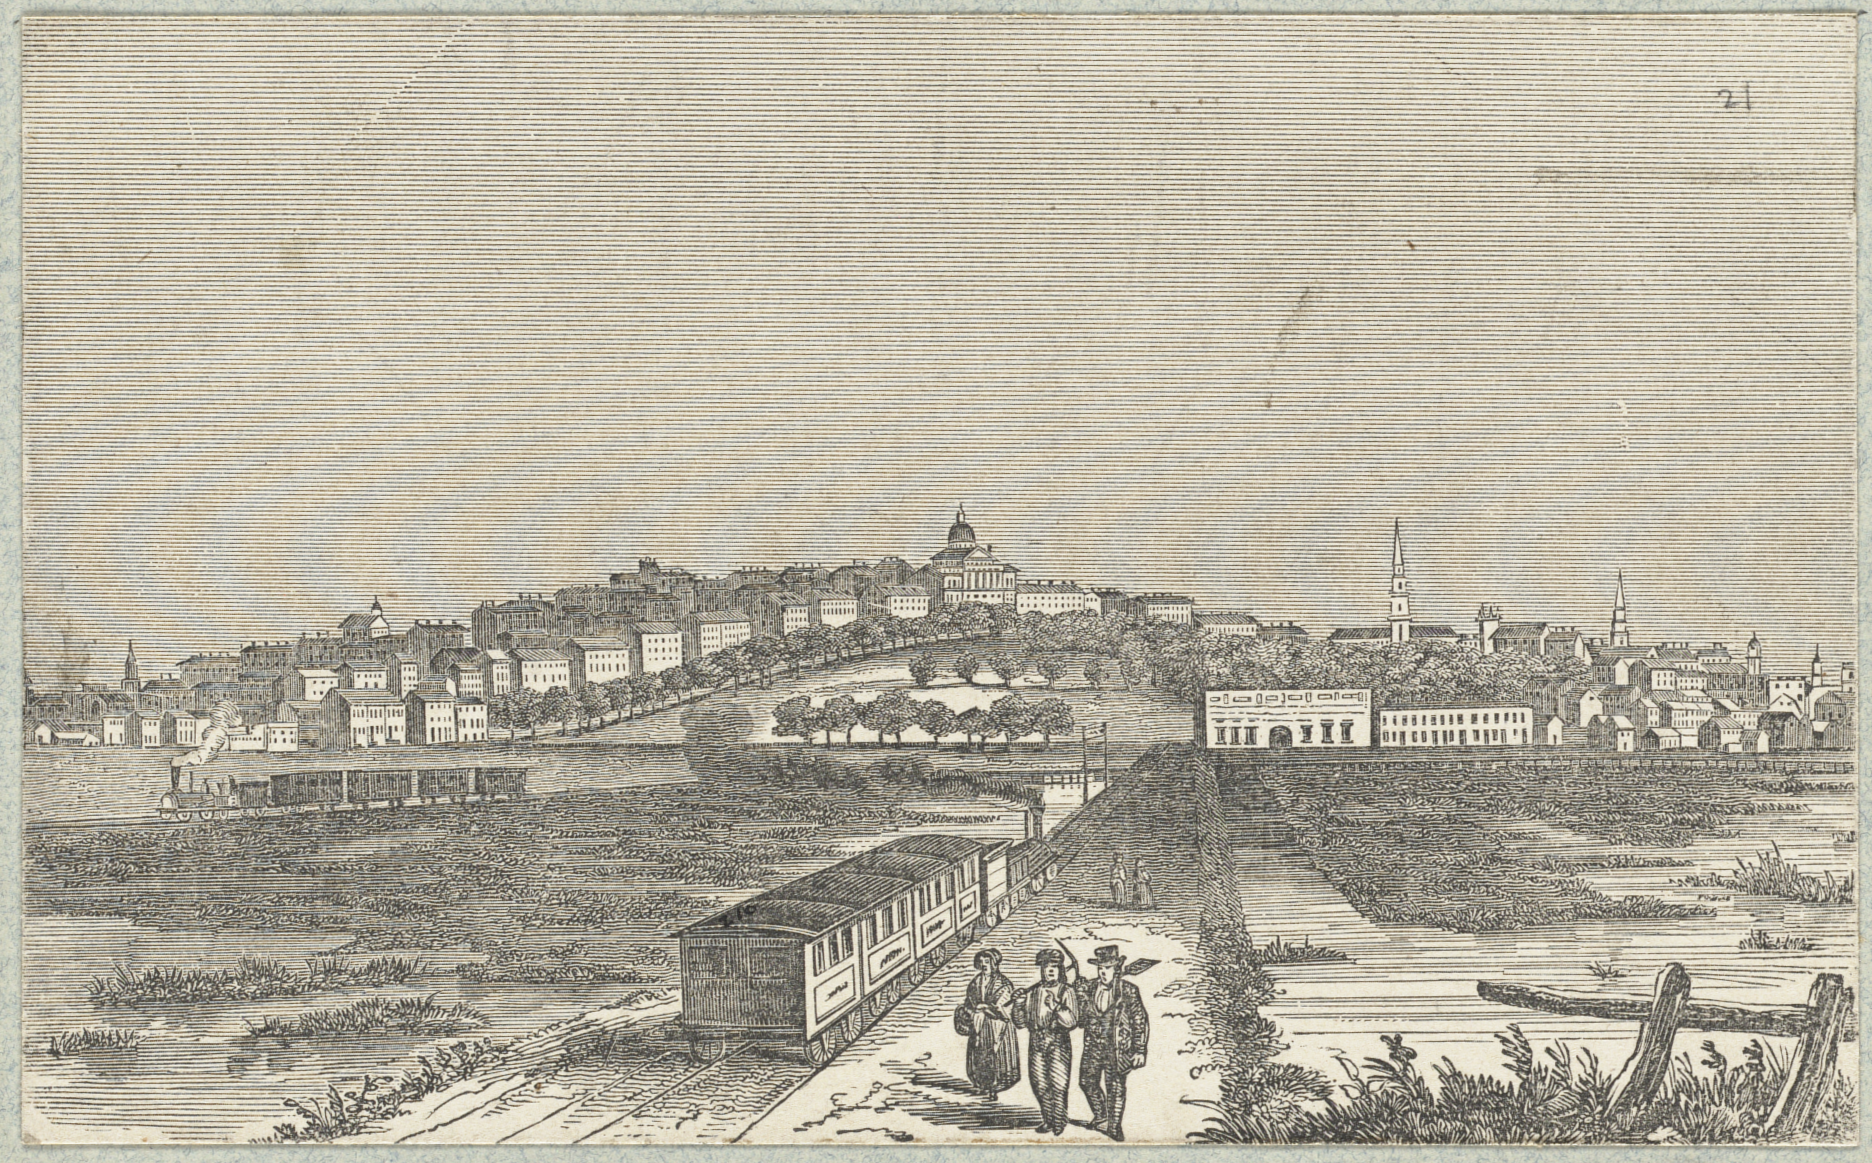
\includegraphics[width=\textwidth]{boston1849}
%	\caption{Wood engraving of Boston in 1849, showing what the city looked like when the O'Briens first arrived.}
%	\label{fig:Boston1849}
%\end{figure}

\begin{figure}
	\centering
	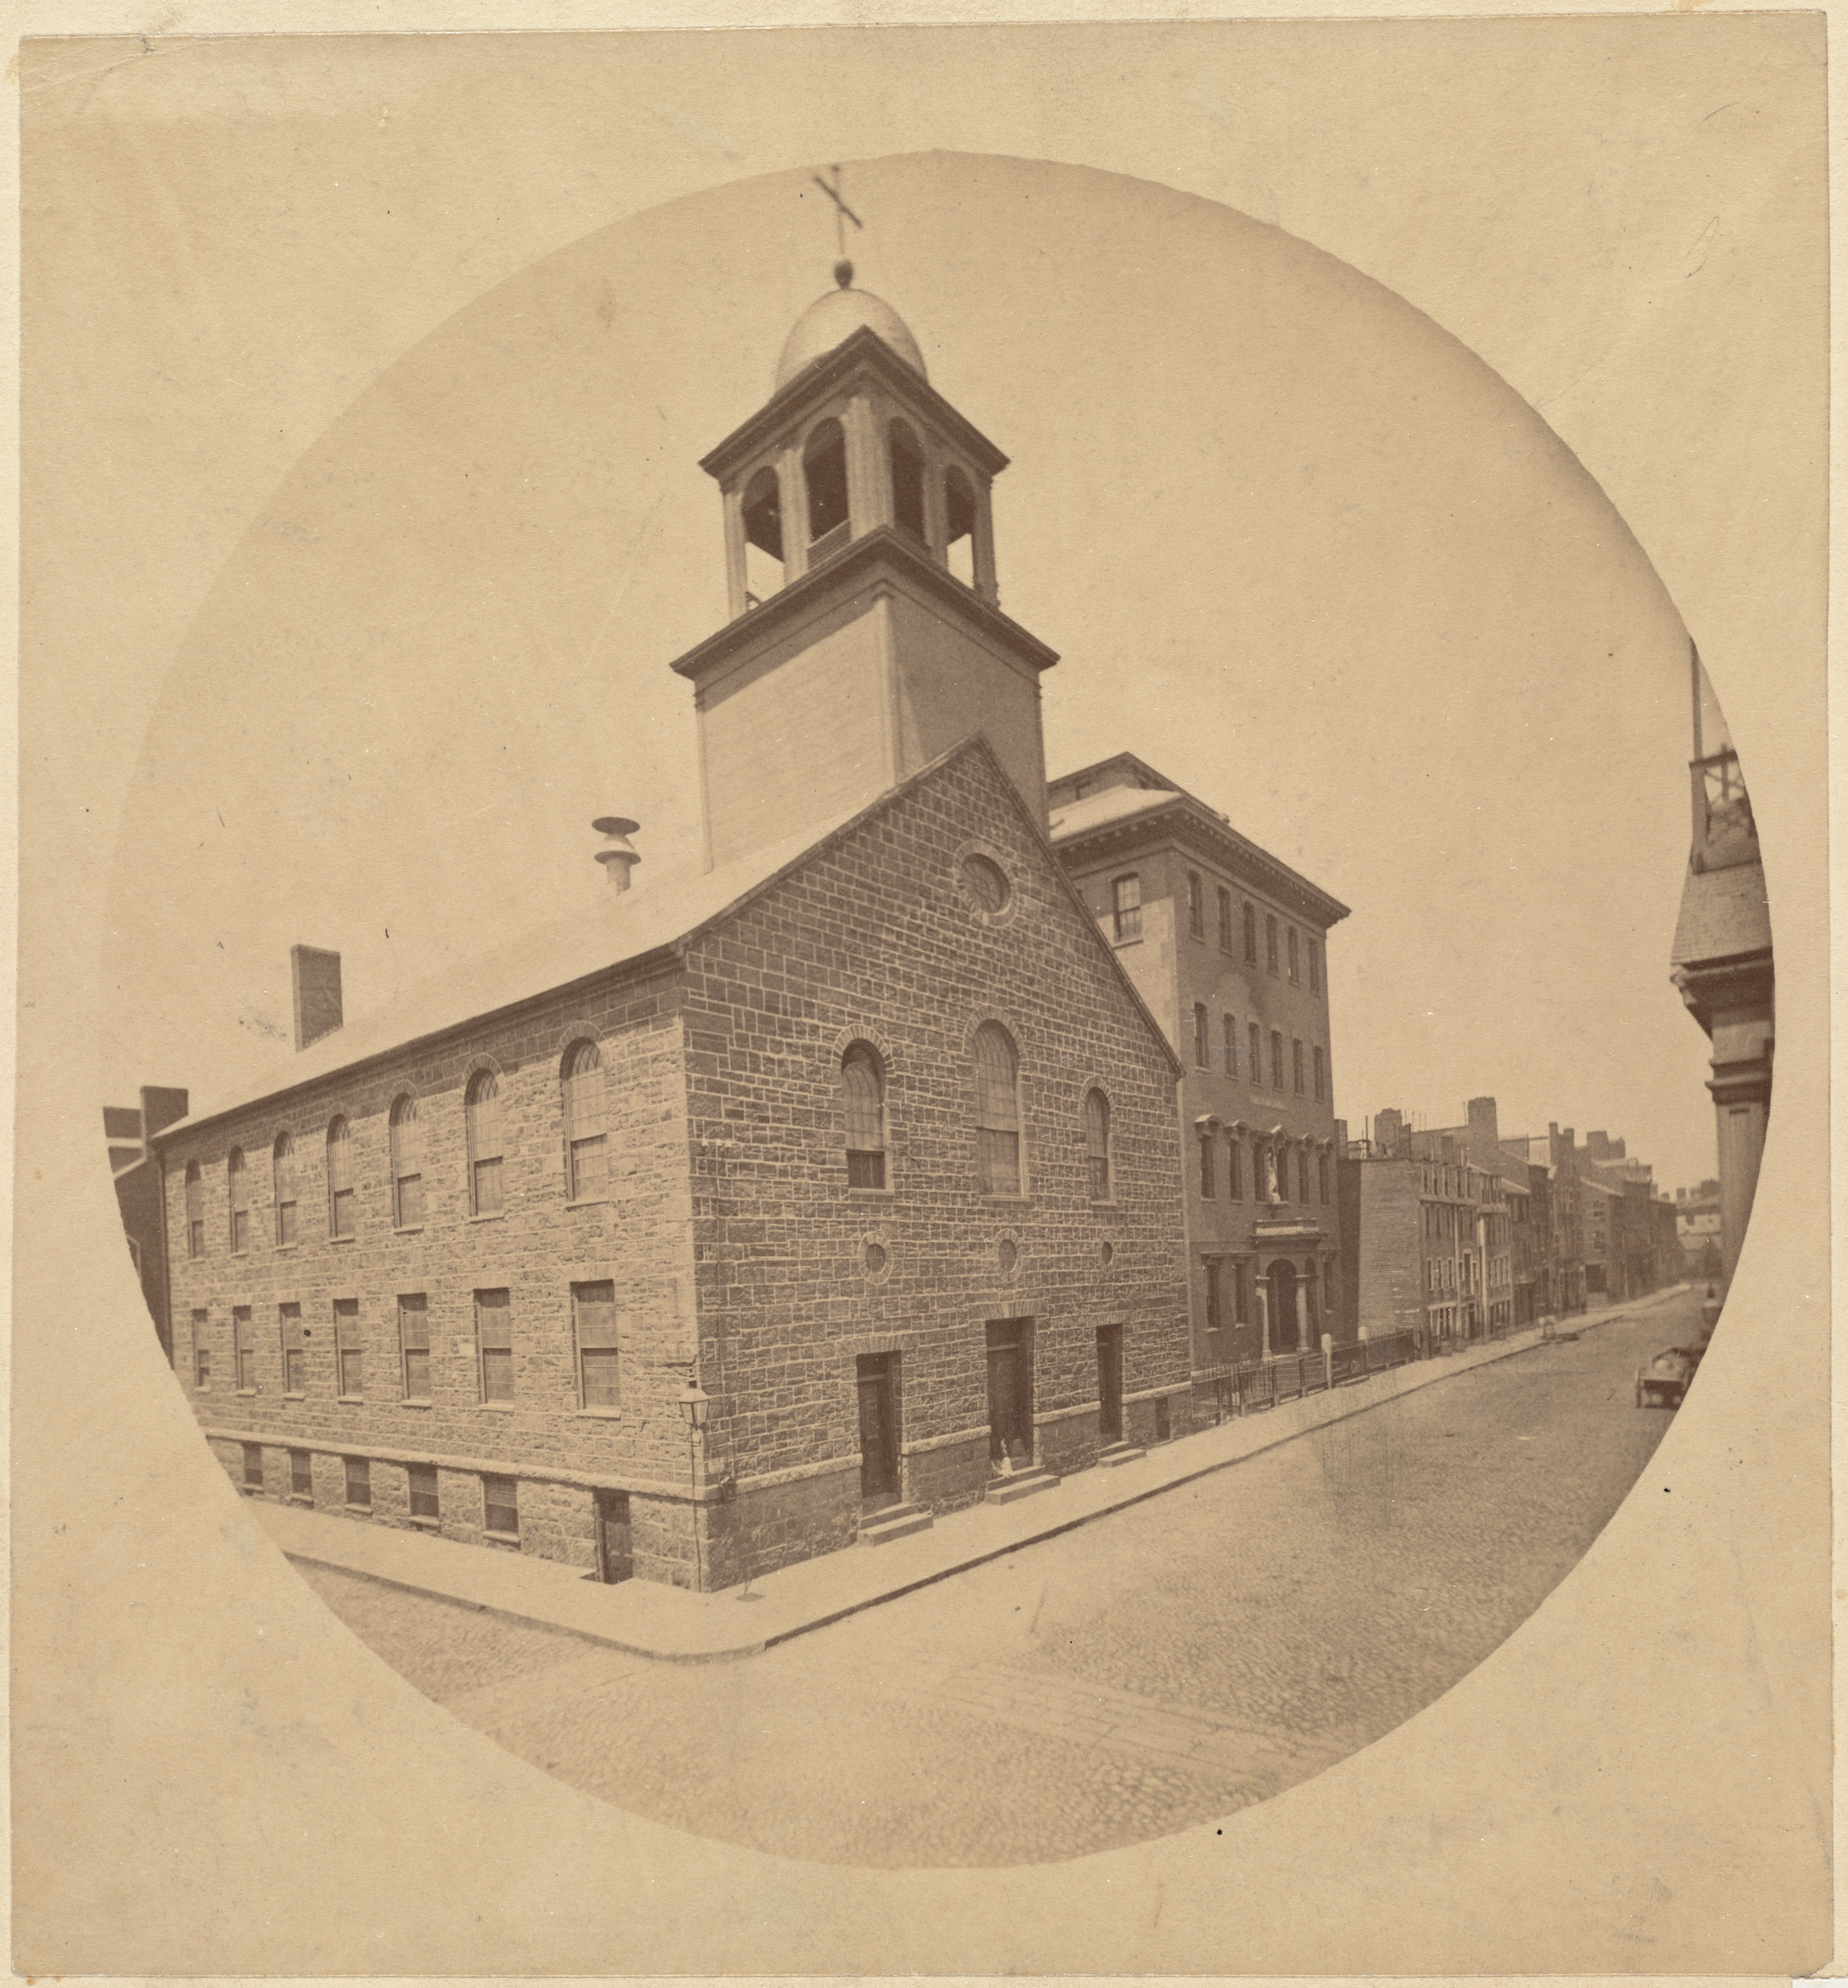
\includegraphics[width=0.5\textwidth]{st_marys}
	\caption{St. Mary's of the Sacred Heart Church.}
	\label{fig:StMarys}
\end{figure}

Irish\index{Irish-Americans} immigrants to Boston\index{Massachusetts!Boston} had difficulty finding steady work, given that they were mostly rural farmers\index{farming} and did not have specialized trade skills.\cite{Ryan:21} Many of them started out by opening a grocery\index{grocer} store in their tenement house or somewhere close by.\cite{Ryan:83} Indeed, John's\index{O'Brien!John\textsuperscript{2}} occupation is listed as ``grocer''\index{grocer} on his son John Joseph's\index{O'Brien!John Joseph\textsuperscript{3} (1861--1938)} birth record.\cite{John3OBrienBirth:1} 

\begin{figure}
	\centering
	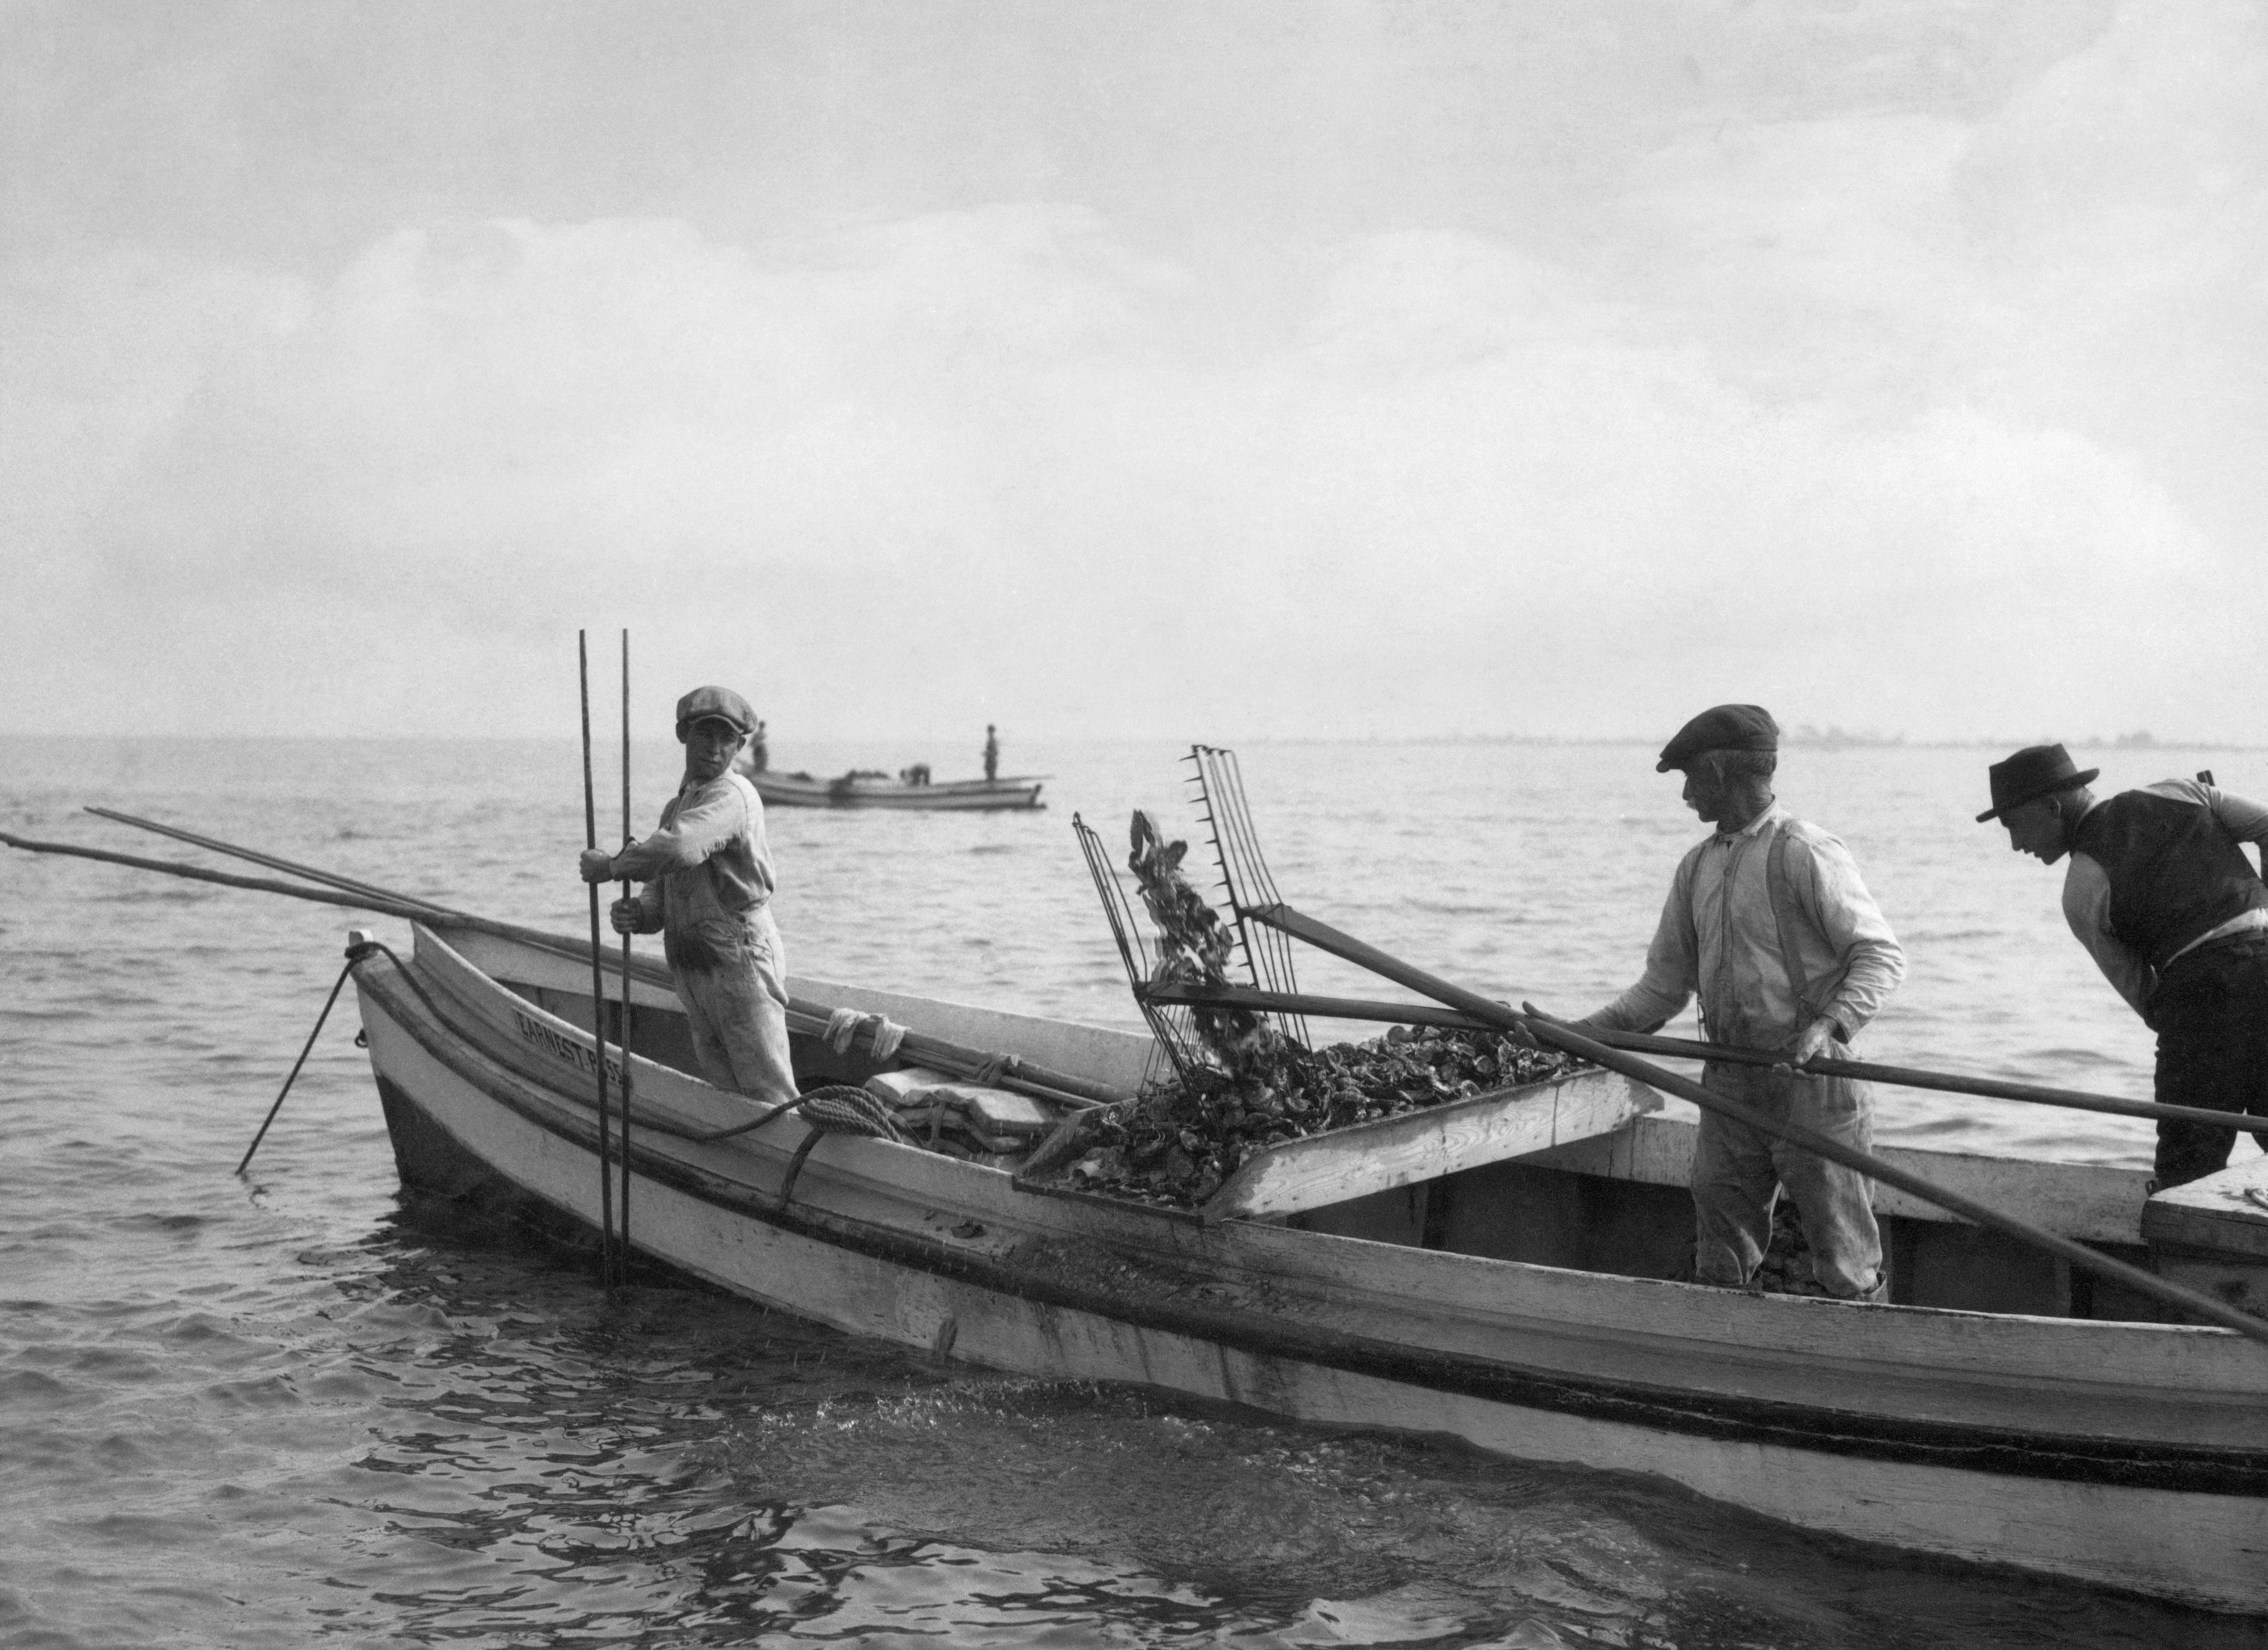
\includegraphics[width=\textwidth]{NatGeo_1238550}
	\caption{Oyster tongers.}\index{oyster harvesting}
	\label{fig:OysterTongers}
\end{figure}

John\index{O'Brien!John\textsuperscript{2}} and his brother Michael\index{O'Brien!Michael\textsuperscript{2}} both worked as oystermen.\index{oyster harvesting}\cite{oysters} Before the advent of industrial-scale dredging operations, the traditional method of oyster harvesting\index{oyster harvesting} used tongs. Oyster tongs consisted of a pair of metal rakes at the end of long wooden shafts. The oysterman\index{oyster harvesting} would use the tongs to scrape oysters off the bottom of the sea bed and manually haul them onto the boat, up to 70 pounds at a time. The boats were small vessels rigged with one or two sails.\cite{Botwick:95} Being an oysterman\index{oyster harvesting} brought a degree of independence for an unskilled laborer. He typically owned his own boat and tackle, shucked the oysters at home to sell locally, and kept all the profits.\cite{MacKenzie:7:1} This changed beginning in the 1870s when steam-powered oyster dredging ships arrived, and packing houses took over the oyster shucking process.\cite{MacKenzie:5} 

The natural oyster beds in the Charles and Mystic Rivers had long been depleted by the time the O'Briens arrived in Boston. Even the oysters around Cape Cod and Rhode Island were diminishing. The Boston oyster dealers replaced the naturally-growing oysters with seed oysters from Long Island Sound and New Jersey at first, and eventually from Virginia, ``planting'' them in the spring and then harvesting the fully-grown oysters in the fall and winter. Ships would bring the oysters into Boston from Wellfleet on Cape Cod, or other planted beds in Narragansett and Buzzard's Bays. Sailors unloaded the oysters at the docks near Fanueil Hall and sold them to local dealers and peddlers.\cite{Ingersoll:27-28} 

Oyster shuckers worked seasonally from September to May. It was a difficult, low-paying job. In 1880 they were paid between 17 and 20 cents per gallon of oysters shucked. Steamships began bringing twice-weekly shipments of opened oysters to Boston from Norfolk, Virginia, making it more difficult to find local employment in the oyster trade.\cite{Ingersoll:30}

It seems that Edward\index{O'Brien!Edward/Edmund\textsuperscript{2}} was the main provider for the O'Brien family\index{O'Brien!family} during the early years in Boston.\index{Massachusetts!Boston} He may have had a successful trade in Ireland\index{Ireland} prior to his arrival in the United States. In 1855 he was housing his father and his sister Abby's\index{Dooley!Abigail\textsuperscript{2} (O'Brien)}\index{O'Brien!Abigail\textsuperscript{2}} family in addition to his own.\cite{Census1855William:1} Edward\index{O'Brien!Edward/Edmund\textsuperscript{2}} purchased a 2-person cemetery plot at North Cambridge Catholic Cemetery\index{North Cambridge Catholic Cemetery} in 1852\cite{CarolGordon:1} and a large 13-person plot at Holy Cross Cemetery\index{Holy Cross Cemetery} in 1880\cite{HolyCrossPlotEdward:1} where many of his family members were buried.

In the early 1870s, most of William's\index{O'Brien!William\textsuperscript{1}} adult children (Edward,\index{O'Brien!Edward/Edmund\textsuperscript{2}} Ann,\index{O'Brien!Ann\textsuperscript{2}}\index{Dailey!Ann\textsuperscript{2} (O'Brien)} Mary,\index{O'Brien!Mary\textsuperscript{2}}\index{Ward!Mary\textsuperscript{2} (O'Brien)} and Michael\index{O'Brien!Michael\textsuperscript{2}}) relocated to East Boston.\index{Massachusetts!Boston!East Boston} John's\index{O'Brien!John\textsuperscript{2}} sons, John Joseph,\index{O'Brien!John Joseph\textsuperscript{3} (1861--1938)} James Edward,\index{O'Brien!James Edward\textsuperscript{3}} and William,\index{O'Brien!William\textsuperscript{3}} moved to Boston's South Cove\index{Massachusetts!Boston!South Cove} neighborhood (now part of Chinatown\index{Massachusetts!Boston!Chinatown}).

John's\index{O'Brien!John\textsuperscript{2}} family was hit particularly hard by tuberculosis.\index{tuberculosis}\index{phthisis|see{tuberculosis}}\index{consumption|see {tuberculosis}} %
%\footnote{The terms ``phthisis'' and ``consumption'' were used at the time to describe what is now called tuberculosis. See I. Berberis, N.L.\ Bragazzi, L.\ Galluzzo, and M. Martini, ``The history of tuberculosis: from the first historical records to the isolation of Koch's bacillus,'' \textit{Journal of Preventive Medicine and Hygiene} 58(1) (March 2017): E9--E12; accessed at \textit{National Center for Biotechnology Information, U.S.\ National Library of Medicine} (\url{https://www.ncbi.nlm.nih.gov/pmc/articles/PMC5432783/} : viewed on 31 Mar 2020).}
Four of his children died of the disease between 1879 and 1889, as did John\index{O'Brien!John\textsuperscript{2}} himself in 1863.\cite{John2OBrienDeath:1} In fact, John's line would have ended if not for his son John Joseph.\index{O'Brien!John Joseph\textsuperscript{3} (1861--1938)} Tuberculosis\index{tuberculosis} disproportionately affected Irish immigrants\index{Irish-Americans} in Boston:\index{Massachusetts!Boston}

\begin{quote}
	\ldots[t]he death rate from consumption\index{tuberculosis} was greatest among the colored, and among the white \ldots it was greatest among those whose mothers were born in Ireland\index{Ireland}\index{Irish-Americans} or who were themselves natives of Ireland, being more than 3 times the corresponding rate for those whose mothers were born in the United States, and almost double the rate for those who were themselves natives of this country.\cite{VitalStatistics}
\end{quote}

Three of Michael's\index{O'Brien!Michael\textsuperscript{2}} sons had jobs working in Boston's\index{Massachusetts!Boston} gas industry.\index{gas industry} Their roles included gas meter maker, meter tester, meter reader, and foreman. The Boston Gas Company\index{Boston Gas Company} constructed a large coal gas plant at Commercial Point\index{Massachusetts!Boston!Commercial Point} in 1882. The company needed to hire a large number of unskilled laborers, and many of them were Irish\index{Irish-Americans} immigrants.\cite{Keating:11} In the early 20th century, these jobs were highly valued, as the company (later called Boston Consolidated Gas)\index{Boston Consolidated Gas} offered employee profit-sharing plans in 1906 and a pension plan in 1919. This provided job stability and wealth for the Irish\index{Irish-Americans} working class.\cite{Keating:20}

The profiles later in this report include details about each descendant of William O'Brien\index{O'Brien!William\textsuperscript{1}} through the 4th generation.

\begin{thebibliography}{999}
	
% Chapter 2: The O'Briens in Boston

\bibitem{Miller:291}
Kerby A.\ Miller, \textit{Emigrants and Exiles} (New York and Oxford, Oxford University Press, 1985), 291.

\bibitem{Miller:292}
Miller, \textit{Emigrants and Exiles}, 292.

\bibitem{Miller:295}
Miller, \textit{Emigrants and Exiles}, 295.

\bibitem{ThomasBaker}
U.S. National Archives and Records Administration (NARA), ``Passenger lists of vessels arriving at New York, 1820-1897,'' NARA microfilm publication M237, roll 81, July 3-27, 1849, list no.\ 882, entries for Mary O'Brien and Michael O'Brien; accessed at ``New York Passenger Lists, 1820-1891,'' database with images, \textit{FamilySearch} (\url{https://familysearch.org/ark:/61903/3:1:939V-5P37-F7} : viewed on 19 Sep 2020), 081 - 3 Jul 1849-27 Jul 1849 > image 123.

\bibitem{OHanlon:35}
John O'Hanlon, \textit{The Irish emigrant's guide for the United States} (Boston: P.\ Donahoe, 1851), 33.

\bibitem{Laxton:9}
Edward Laxton, \textit{The Famine Ships: The Irish Exodus to America 1846-51} (New York: Henry Holt and Company, 1997), 9. 

\bibitem{MorningAdvertiser}
``POLICE COURTS,'' \textit{Morning Advertiser} (London), 2 Nov 1844; accessed at ``British Newspapers,'' database with images, \textit{Findmypast} (\url{https://search.findmypast.com/search/british-newspapers} : viewed on 19 Sep 2020).

\bibitem{OHanlon:33}
O'Hanlon, \textit{The Irish emigrant's guide for the United States}, 33.

\bibitem{Chascay:1}
``Registers of Passengers Arriving in Massachusetts Ports 1848-1891,'' Massachusetts State Archives, HS 3.02 1990X, record of 27 Jun 1851, vessel \textit{Chascay}, entries for Edmund O'Brien and family; accessed at ``Massachusetts, United States Records,'' images, FamilySearch (\url{https://www.familysearch.org/ark:/61903/3:1:3Q9M-CSVN-998J-W} : viewed on 11 Nov 2020), image 793. On this page the ship name is written as ``Chascay'' but on the previous pages appears as ``Chasca.''

\bibitem{Chascay2:1}
Advertisement for the ship Chasca, \textit{Gore's Liverpool General Advertiser}, 1 May 1851, p.\ 2; accessed at the British newspaper collection, database with images, Findmypast (\url{https://search.findmypast.com/search/british-newspapers} : viewed on 11 Nov 2020).

\bibitem{Chascay:2}
``Registers of Passengers Arriving in Massachusetts Ports 1848-1891,'' Massachusetts State Archives, HS 3.02 1990X, record of 27 Jun 1851, vessel \textit{Chasca}/\textit{Chascay}.

\bibitem{ChascaCard}
``\textit{Chasca} (Clipper Bark), undated,'' Sailing Ship Card Collection, Phillips Library (Rowley, Mass.), call number MSS 470, box 2, folder 34; \url{https://pem.as.atlas-sys.com/repositories/2/archival_objects/54001}; ``Registers of Passengers Arriving in Massachusetts Ports 1848-1891,'' Massachusetts State Archives, HS 3.02 1990X, record of 27 Jun 1851, vessel \textit{Chasca}/\textit{Chascay}.

\bibitem{Chascay:4}
``Registers of Passengers Arriving in Massachusetts Ports 1848-1891,'' Massachusetts State Archives, HS 3.02 1990X, record of 27 Jun 1851, vessel \textit{Chasca}/\textit{Chascay}.

\bibitem{Ryan:41}
Dennis P.\ Ryan, \textit{Beyond the Ballot Box: A Social History of the Boston Irish, 1845--1917} (Amherst: University of Massachusetts Press, 1989), pp.\ 41--42.

\bibitem{John2OBrienCivilMarriage:1}
Massachusetts Vital Records, marriage records, 1853, p.\ 156, no.\ 2642, John O'Brien and Mary Mahoney; accessed at ``Massachusetts, Marriage Records, 1840-1915,'' database with images, \textit{Ancestry.com} (\url{https://www.ancestry.com/search/collections/2511/} : viewed on 31 Mar 2020), \_Up Through 1910 > 1853 > image 779.

\bibitem{Census1880Edward:1}
1880 U.S. census, Suffolk County, Massachusetts, population schedule, East Boston, Enumeration District (ED) 576, p.\ 24, dwelling 153, family 267, Edward O'Brian household; accessed at ``1880 United States Federal Census,'' database with images, \textit{Ancestry.com} (\url{https://www.ancestry.com/search/collections/6742/} : viewed on 2 Apr 2020), Massachusetts > Suffolk > Boston > 576 > image 24.

\bibitem{Protestantism}
Dennis P.\ Ryan, \textit{Beyond the Ballot Box: A Social History of the Boston Irish, 1845--1917} (Amherst: University of Massachusetts Press, 1989), p.\ 61; Michael Quinlan, \textit{Irish Boston: A Lively Look at Boston's Colorful Irish Past}, second edition (Guilford: Globe Pequot Press, 2013), p.\ 58.

\bibitem{NorthEndAddresses}
For North End addresses, see: civil birth record of William\textsuperscript{3} O'Brien at 3 Morton St. in 1854; birth record of Mary\textsuperscript{3} O'Brien at Hanover St.\ in 1856; death record of William O'Brien at 207 North St.\ in 1856; death record of Anna O'Brien at 207 North St.\ in 1857; birth record of James\textsuperscript{3} O'Brien at 9 Morton St.\ in 1858; birth record of John Joseph\textsuperscript{3} O'Brien at 35 Fleet St.\ in 1861; 1862 birth of Margaret\textsuperscript{3} O'Brien at 34 Fleet St.\ in 1862; death of Margaret\textsuperscript{3}  O'Brien at 34 Fleet St.\ in 1863; death of Anna\textsuperscript{3} O'Brien at 37 Clark St. in 1866; city directory showing Thomas Bowser living at 450 Hanover St.\ in 1870.

\bibitem{Todisco:29}
Paul J.\ Todisco, \textit{Boston's First Neighborhood: The North End} (Boston: Boston Public Library Duplicating Department, 1976), p.\ 29.

\bibitem{Goldfeld:102}
Alex R.\ Goldfeld, \textit{The North End: A Brief History of Boston's Oldest Neighborhood} (Charleston: The History Press, 2009), p.\ 102.

\bibitem{tuberculosis}
Goldfeld, \textit{The North End: A Brief History of Boston's Oldest Neighborhood}, 103; Todisco, \textit{Boston's First Neighborhood: The North End}, 21; Ryan, \textit{Beyond the Ballot Box: A Social History of the Boston Irish, 1845--1917}, 48.

\bibitem{Todisco:26}
Todisco, \textit{Boston's First Neighborhood: The North End}, 26.

\bibitem{John2OBrienMarriage:1}
St. Mary (Boston) Marriages, 1836-1854, p.\ 205, John O'Brien and Mary Mahoney; accessed at ``Roman Catholic Archdiocese of Boston Records, 1789-1920,'' database with images, \textit{AmericanAncestors.org} (\url{https://www.americanancestors.org/DB2726/i/54105/205/1424477986} : viewed on 31 Mar 2020).

\bibitem{MoonSt}
Goldfeld, \textit{The North End: A Brief History of Boston's Oldest Neighborhood}, 101; James S.\ Sullivan, ed., \textit{One hundred years of progress: a graphic, historical, and pictorial account of the Catholic Church of New England, Archdiocese of Boston} (Boston and Portland: Illustrated Publishing Company, 1895), p.\ 128; accessed at \textit{Internet Archive} (\url{https://archive.org/details/onehundredyearso00bost} : viewed on 13 Sep 2020).

\bibitem{Sullivan:128:2}
Sullivan, \textit{One hundred years of progress: a graphic, historical, and pictorial account of the Catholic Church of New England, Archdiocese of Boston}, p.\ 128.

\bibitem{RobertFernaldMarriage:1}
Massachusetts Vital Records, marriage records, 1873, no.\ 2971, Robert Fernald and Margaret Simonds; accessed at ``Massachusetts, Marriage Records, 1840-1915,'' database with images, \textit{Ancestry.com} (\url{https://www.ancestry.com/search/collections/2511/} : viewed on 11 Apr 2020), \_Up Through 1910 > 1873 > image 983. Margaret's parents' names are incorrectly listed as ``John'' and ``Nancy Dooley.''

\bibitem{Ryan:21}
Ryan, \textit{Beyond the Ballot Box: A Social History of the Boston Irish, 1845--1917}, 21.

\bibitem{Ryan:83}
Ryan, \textit{Beyond the Ballot Box: A Social History of the Boston Irish, 1845--1917}, 83.

\bibitem{John3OBrienBirth:1}
Massachusetts Vital Records, birth records, 1861, p.\ 11, no.\ 471, John O'Brien; accessed at ``Massachusetts, Birth Records, 1840-1915,'' database with images, \textit{Ancestry.com} (\url{https://www.ancestry.com/search/collections/5062/} : viewed on 31 Mar 2020), \_up through 1910 > 1861 > image 909.

\bibitem{oysters}
Massachusetts Vital Records, birth records, 1883, p.\ 38, no.\ 1669, Edward Francis O'Brien; accessed at ``Massachusetts, Birth Records, 1840-1915,'' database with images, \textit{Ancestry.com} (\url{https://www.ancestry.com/search/collections/5062/} : viewed on 7 Apr 2020), \_up through 1910 > 1883 > image 1071.

Sampson, Murdock, and Company, compilers, \textit{The Boston Directory} (Boston: Sampson, Murdock, and Company, 1886), p.\ 888, Michael O'Brien; accessed at ``U.S.\ City Directories, 1822-1995,’’ \textit{Ancestry.com} (\url{https://www.ancestry.com/search/collections/2469/} : viewed on 7 Apr 2020), Massachusetts > Boston > 1886 > Boston, Massachusetts, City Directory, 1886 > image 535.

Adams, Sampson, \& Company, compilers, \textit{The Boston Directory} (Boston: Adams, Sampson, \& Company, 1861), p.\ 355, John O'Brien at 35 Fleet St.; accessed at ``The Boston Directory, 1789 to 1900,'' \textit{Boston Athenaeum Digital Collections} (\url{https://cdm.bostonathenaeum.org/digital/collection/p16057coll32/id/93/rec/11} : viewed on 25 Jul 2020), Home > Boston Directory, 1789 to 1901 > 1861, Boston directory > image 337.

\bibitem{Botwick:95}
Bradford Botwick and Debra A.\ McClane, ``Landscapes of Resistance: A View of the Nineteenth-Century Chesapeake Bay Oyster Fishery,''  \textit{Historical Archaeology}, 2005, vol.\ 39, no.\ 3, Landscapes of Industrial Labor (2005), 95, accessed at \textit{JSTOR} (\url{https://www.jstor.org/stable/25617272} : viewed on 17 Sep 2020)

\bibitem{MacKenzie:7:1}
Clyde L.\ MacKenzie Jr., ``History of Oystering in the United States and Canada, Featuring the Eight Greatest Oyster Estuaries,'' \textit{Marine Fisheries Review}, 58(4), 1996, 7; Botwick and McClane, ``Landscapes of Resistance: A View of the Nineteenth-Century Chesapeake Bay Oyster Fishery,''  \textit{Historical Archaeology}, 2005, vol.\ 39, no.\ 3, 96.

\bibitem{MacKenzie:5}
MacKenzie, ``History of Oystering in the United States and Canada, Featuring the Eight Greatest Oyster Estuaries,'' \textit{Marine Fisheries Review}, 58(4), 1996, 5--7.

\bibitem{Ingersoll:27-28}
Ernest Ingersoll, \textit{The Oyster-Industry}, U.S.\ Department of the Interior (Washington, D.C.: Government Printing Office, 1881), 27--28.

\bibitem{Ingersoll:30}
Ingersoll, \textit{The Oyster-Industry}, 30.

\bibitem{Census1855William:1}
1855 Massachusetts state census, Suffolk County, population schedule, Boston, ward 1, p.\ 60 (left side), dwelling [blank], family 549, for William O'Brien in Edward O'Brien household; accessed at ``Massachusetts, State Census, 1855,'' database with images, \textit{Ancestry.com} (\url{https://www.ancestry.com/search/collections/4472/} : viewed on 29 Mar 2020), Suffolk > Boston Ward 01 > image 33.

\bibitem{CarolGordon:1}
Carol Gordon, Catholic Cemetery Association of the Archdiocese of Boston, emails to Gavin E.\ O'Brien in Apr.\ 2019.

\bibitem{HolyCrossPlotEdward:1}
The Catholic Cemetery Association of the Archdiocese of Boston, Owner Profile, owner ID C15-61458 (Edward O'Brien) at Holy Cross Cemetery, printed 18 Jul 2019.

\bibitem{John2OBrienDeath:1}
Massachusetts Vital Records, death records, 1863, p.\ 49, no.\ 1270, John O'Brien; accessed at ``Massachusetts, Death Records, 1841-1915,'' database with images, \textit{Ancestry.com} (\url{https://www.ancestry.com/search/collections/2101/} : viewed on 31 Mar 2020), \_Pre 1903 > 1863 > image 756. Cause of death: phthisis.

\bibitem{VitalStatistics}
John S. Billings, M.D., United States Census Office, \textit{Vital statistics of Boston and Philadelphia covering a period of six years ending May 31, 1890} (1895), 30; accessed at \textit{Internet Archive} (\url{https://archive.org/details/vitalstatistics00shungoog/page/n22/mode/2up} : viewed on 2 Apr 2020). 

\bibitem{Keating:11}
Suzanne Keating, \textit{Illuminations: The History of the Boston Gas Company} (Rockland: InterCity Press, 1999), 11.

\bibitem{Keating:20}
Keating, \textit{Illuminations: The History of the Boston Gas Company}, 20.

\end{thebibliography}

\chapter{DNA Evidence}

O'Brien\index{O'Brien!surname} is the Anglicized spelling of the surname \textit{Ua Briain} in Classical Irish, and \textit{\'{O} Briain} in Modern Irish. The \textit{Ua} or \textit{\'{O}} part of the name means a ``grandson'' or generally any descendant of the named person. In this case, O'Brien derives from the first name of Brian Boru\index{Boru!Brian} (born c. 941 and died 23 Apr 1014), High King of Ireland.\index{Ireland} Boru's descendants formed one of the major dynasties in Ireland.\index{Ireland}\cite{BoruHistorical}

Brian Boru\index{Boru!Brian} was born a member of the D\'{a}l gCais clan (Dalcassians).\index{D\'{a}l gCais (clan)}\index{Dalcassians|see{D\'{a}l gCais (clan)}} This clan controlled much of what is now County Clare\index{Ireland!County Clare} in Ireland.\index{Ireland}\cite{BoruEarlyHistory} Due to modern genetic testing, it is possible to determine whether a living person is a descendant of Brian Boru,\index{Boru!Brian} a member of his clan, or an unrelated O'Brien who came from a family that adopted the surname. This is facilitated by the Y-DNA\index{DNA!Y-DNA} testing of Brian Boru's\index{Boru!Brian} living direct descendant, Sir Conor O'Brien,\index{O'Brien!Conor} 18th Baron Ichiquin.\cite{GGI:1}\index{Baron Inchiquin}

Unlike other chromosomes, the Y chromosome\index{DNA!Y-DNA} is passed from father to son without significant recombination. This means that a living man's Y-DNA\index{DNA!Y-DNA} is nearly identical to that of his direct male line ancestor from many generations in the past. While rare, mutations on the Y chromosome do occur. These variations are called single nucleotide polymorphisms, or SNPs.\index{DNA!SNPs} It is possible to map groups of people onto branches of a tree based on the SNPs\index{DNA!SNPs} they have in common. These branches are known as haplogroups,\index{DNA!Haplogroups} and they're named after the Y-DNA\index{DNA!Y-DNA} mutation that defines them.\cite{Bettinger}

The Y-DNA\index{DNA!Y-DNA} testing of Sir Conor O'Brien\index{O'Brien!Conor} has revealed that Brian Boru's\index{Boru!Brian} Dalcassian\index{D\'{a}l gCais (clan)} clan and its descendants are located within the R-L226 haplogroup.\index{DNA!R-L226 haplogroup} Furthermore, Brian Boru's\index{Boru!Brian} defining mutation places him and his descendants in the sub-group of R-L226\index{DNA!R-L226 haplogroup} known as FGC5659.\index{DNA!FGC5659 haplogroup} There is another group of non-Dalcassian\index{D\'{a}l gCais (clan)} O'Briens known as the ``Northwest Irish/Lowland Scots'' O'Briens,\index{Northwest Irish/Lowland Scots O'Briens} who are in haplogroup R-M222.\index{DNA!R-M222 haplogroup}\cite{GGI:2}

%\begin{figure}
%	\centering
%	\includegraphics[width=\textwidth]{ydna}
%	\caption{}
%\end{figure}

A Y-DNA\index{DNA!Y-DNA} test of William O'Brien's\index{O'Brien!William\textsuperscript{1}} male line\cite{BigY} reveals that there is no relation to either the Dalcassian\index{D\'{a}l gCais (clan)} or Northwest Irish O'Briens.\index{Northwest Irish/Lowland Scots O'Briens} William's\index{O'Brien!William\textsuperscript{1}} branch is located within haplogroup R-Y11179.\index{DNA!R-Y11179 haplogroup} This haplogroup does not have ancient Irish origins but can be traced back to the Anglo-Norman\index{Anglo-Normans} family with the surname ``Barry''\index{Barry surname} that occupied large parts of County Cork\index{Ireland!County Cork} subsequent to the English\index{England} invasion of Ireland\index{Ireland} in the 1100s.\cite{BarrymoreDNA:9} More recent research indicates that these Barrys\index{Barry surname} were probably from the Hainaut\index{Belgium!Hainaut} region of what is now Belgium, rather than French Normandy.\index{France!Normandy}\cite{BarrymoreDNA:2-4}

Several websites provide age estimates to determine when William O'Bri\-en's\index{O'Brien!William\textsuperscript{1}} line may have split off from the Barry family.\index{Barry surname} The closest match on FamilyTreeDNA (FTDNA)\index{FamilyTreeDNA} is a man with a Barry surname.\index{Barry surname} FTDNA's\index{FamilyTreeDNA} ``TiP Report'' estimates that the Barry\index{Barry surname} match and William O'Brien's\index{O'Brien!William\textsuperscript{1}} descendant have a common ancestor within the past 8 generations at 60.41\% likelihood, within 12 generations at 90.11\% likelihood, and within 18 generations at 98.28\% likelihood.\cite{TiP} On the website \textit{YFull},\index{YFull} which allows uploading Y-DNA\index{DNA!Y-DNA} kits for additional analysis, the closest match is the same Barry\index{Barry surname} individual from the previous comparison. YFull\index{YFull} predicts that the two matches have a most recent common ancestor at a median of 425 years ago with 95\% certainty, placing the common ancestor around the year 1600.\cite{YFull}

Somewhere in William O'Brien's\index{O'Brien!William\textsuperscript{1}} ancestry, the O'Brien name\index{O'Brien!surname} was assigned to (or adopted by) a man of Barry\index{Barry surname} descent. This is known as a non-paternity event (NPE).\index{non-paternity event (NPE)} It is likely impossible to determine when or how this occurred, as useful records in Ireland\index{Ireland} rarely go back far enough past the early 1800s. However, the Barry\index{Barry surname} family had a major presence in the area where William\index{O'Brien!William\textsuperscript{1}} came from, receiving grants of land in County Cork\index{Ireland!County Cork} from the English\index{England} king and the title Earl of Barrymore.\index{Earl of Barrymore}\cite{BarrymoreDNA:4} More information may arise as additional men submit Y-DNA\index{DNA!Y-DNA} tests and the timeline for the O'Brien/Barry split can be further narrowed. It is also important to note that the Y-DNA\index{DNA!Y-DNA} results only pertain to the direct male line. William's\index{O'Brien!William\textsuperscript{1}} descendants still have Irish roots, owing to the Irish spouses of his children. William's\index{O'Brien!William\textsuperscript{1}} own mother is unknown, but it's quite likely she had ancestral Irish origins.

\chapter{First Generation}
\section{William O'Brien and Mary Sexton}\label{per:William1OBrien}

\MainPerson{William\textsuperscript{1} O'Brien}\index{O'Brien!William\textsuperscript{1}|bb} was born probably in County Cork, Ireland,\index{Ireland!County Cork} about 1791.\cite{Census1855William} He died in Boston, Massachusetts,\index{Massachusetts!Boston} 28 December 1856,\cite{William1OBrienDeath} and was buried at North Cambridge Catholic Cemetery,\index{North Cambridge Catholic Cemetery} Cambridge, Massachusetts.\index{Massachusetts!Cambridge}\cite{DianaBerberenaLetter1} He married, likely in County Cork,\index{Ireland!County Cork} \MainPerson{Mary Sexton}.\index{Sexton!Mary\textsuperscript{1}}\index{O'Brien!Mary\textsuperscript{1} (Sexton)}\cite{Michael2OBrienDeath,Abigail2OBrienDeath,Ann2OBrienDeath,Mary2OBrienDeath} No further information about Mary\index{Sexton!Mary\textsuperscript{1}}\index{O'Brien!Mary\textsuperscript{1} (Sexton)} is known.

William\index{O'Brien!William\textsuperscript{1}|bb} left Ireland\index{Ireland} at age 60 with his son Edward,\index{O'Brien!Edward/Edmund\textsuperscript{2}} daughter-in-law Bridget,\index{Linehan/Linnehan!Bridget}\index{O'Brien!Bridget (Linnehan)} daughter Abby,\index{O'Brien!Abigail\textsuperscript{2}}\index{Dooley!Abigail\textsuperscript{2} (O'Brien)} and granddaughters MargaretMargaret\textsuperscript{3}\index{Dooley!Margaret\textsuperscript{3}}\index{Fernald!Margaret\textsuperscript{3} (Dooley) (Simonds)}\index{Simonds!Margaret\textsuperscript{3} (Dooley)} and Hannah.\index{Dooley!Hannah/Hanora\textsuperscript{3}}\index{Cooney!Hannah/Hanora\textsuperscript{3} (Dooley)} They sailed on the ship \textit{Chasca}\cite{Chascay2}\index{Chasca (ship)} from Liverpool, England,\index{England!Liverpool} arriving in Boston\index{Massachusetts!Boston} on 27 June 1851 after a 47-day voyage.\cite{Chascay}

In 1855, William\index{O'Brien!William\textsuperscript{1}|bb} was living in Boston's North End\index{Massachusetts!Boston!North End} neighborhood with Edward\index{O'Brien!Edward/Edmund\textsuperscript{2}} and Abby.\index{O'Brien!Abigail\textsuperscript{2}}\index{Dooley!Abigail\textsuperscript{2} (O'Brien)}\cite{Census1855William,Wards} William's\index{O'Brien!William\textsuperscript{1}|bb} wife Mary\index{Sexton!Mary\textsuperscript{1}}\index{O'Brien!Mary\textsuperscript{1} (Sexton)} does not appear in any census records from this time. She may have died in Ireland\index{Ireland} before 1851.

William\index{O'Brien!William\textsuperscript{1}|bb} lived in Boston\index{Massachusetts!Boston} for five years before dying of ``pleurisy.''\index{pleurisy} He was living at 207 North Street\index{Massachusetts!Boston!North St.} in the North End\index{Massachusetts!Boston!North End} at the time.\cite{William1OBrienDeath}

\begin{KidsIntro}
	Children of William\textsuperscript{1} O'Brien\index{O'Brien!William\textsuperscript{1}|bb} and Mary (Sexton) O'Brien,\index{Sexton!Mary\textsuperscript{1}}\index{O'Brien!Mary\textsuperscript{1} (Sexton)} all likely born in Watergrasshill:\index{Ireland!Watergrasshill, County Cork}
\end{KidsIntro}

\begin{Kids}
	\KidNum{}{i.}\KidName{Ann\textsuperscript{2} O'Brien},\index{O'Brien!Ann\textsuperscript{2}}\index{Dailey!Ann\textsuperscript{2} (O'Brien)} b.\ abt.\ 1813;\cite{1880CensusAnn} d.\ 23 Sept.\ 1898;\cite{Ann2OBrienDeath} m.\ \KidName{Michael Dailey}.\index{Dailey!Michael}\cite{Ann2OBrienDeath} Unknown if she had any children. She does not appear until the 1880 census, when she was living with her brother Edward.\index{O'Brien!Edward/Edmund\textsuperscript{2}} She may have arrived in the U.S. sometime between 1870--1880. No record of husband Michael Dailey\index{Dailey!Michael} being in the U.S.
	
	\KidNum{\ref{per:Abigail2OBrien}}{ii.}\KidName{Abigail ``Abby'' O'Brien},\index{O'Brien!Abigail\textsuperscript{2}}\index{Dooley!Abigail\textsuperscript{2} (O'Brien)} b.\ abt.\ 1815 or 1825; m.\ \KidName{Michael Dooley}.\index{Dooley!Michael}
	
	\KidNum{\ref{per:John2OBrien}}{iii.}\KidName{John O'Brien},\index{O'Brien!John\textsuperscript{2}} b.\ abt.\ 1820; m.\ 20 Nov.\ 1853, \KidName{Mary Mahoney}.\index{Mahoney/Mahony!Mary}\index{O'Brien!Mary (Mahoney)}
	
	\KidNum{\ref{per:Edward2OBrien}}{iv.}\KidName{Edward O'Brien},\index{O'Brien!Edward/Edmund\textsuperscript{2}} b.\ 10 Oct.\ 1822; m.\ \KidName{Bridget Linnehan}.\index{Linehan/Linnehan!Bridget}\index{O'Brien!Bridget (Linnehan)}
		
	\KidNum{\ref{per:Mary2OBrien}}{v.}\KidName{Mary O'Brien},\index{O'Brien!Mary\textsuperscript{2}}\index{Ward!Mary\textsuperscript{2} (O'Brien)} b.\ abt.\ 1828; m.\ 31 Oct.\ 1850, \KidName{David Ward}.\index{Ward!David (husband of Mary (O'Brien))}
	
	\KidNum{\ref{per:Michael2OBrien}}{vi.}\KidName{Michael O'Brien},\index{O'Brien!Michael\textsuperscript{2}} b.\ 15 Dec.\ 1832; m.\ (1) 10 July 1854, \KidName{Bridget Colbert};\index{Colbert!Bridget}\index{O'Brien!Bridget (Colbert)} m.\ (2) 19 April 1874, \KidName{Mary Field}.\index{Field!Mary}\index{O'Brien!Mary (Field)}\index{Feely, Mary!see {Field, Mary}}
			
\end{Kids}

\begin{thebibliography}{999}

% Chapter 4: Generation 1

\bibitem{Census1855William:2}
1855 Massachusetts state census, Suffolk County, population schedule, Boston, ward 1, p.\ 60 (left side), dwelling [blank], family 549, for William O'Brien in Edward O'Brien household; accessed at ``Massachusetts, State Census, 1855,'' database with images, \textit{Ancestry.com} (\url{https://www.ancestry.com/search/collections/4472/} : viewed on 29 Mar 2020), Suffolk > Boston Ward 01 > image 33.

\bibitem{William1OBrienDeath:1}
Massachusetts Town and Vital Records, Death Records, 1856, no.\ 4206, William O'Brien; accessed at ``Massachusetts, Town and Vital Records, 1620-1988,'' database with images, \textit{Ancestry.com} (\url{https://www.ancestry.com/search/collections/2495/} : viewed on 29 Mar 2020), Boston > Deaths, 1856 > image 96.

\bibitem{DianaBerberenaLetter1:1}
Diana Berberena, Catholic Cemetery Association of the Archdiocese of Boston, letter to Gavin E.\ O'Brien, dated 27 May 2019.

\bibitem{Chascay:5}
``Registers of Passengers Arriving in Massachusetts Ports 1848-1891,'' Massachusetts State Archives, HS 3.02 1990X, record of 27 Jun 1851, vessel \textit{Chascay}, entries for Edmund O'Brien and family; accessed at ``Massachusetts, United States Records,'' images, FamilySearch (\url{https://www.familysearch.org/ark:/61903/3:1:3Q9M-CSVN-998J-W} : viewed on 11 Nov 2020), image 793.

Advertisement for the ship Chasca, \textit{Gore's Liverpool General Advertiser}, 1 May 1851, p.\ 2; accessed at the British newspaper collection, database with images, Findmypast (\url{https://search.findmypast.com/search/british-newspapers} : viewed on 11 Nov 2020).

\bibitem{Census1855William:3}
1855 Massachusetts state census, Suffolk Co., pop.\ sch., Boston, p.\ 60 (left side), dwell.\ [blank], fam.\ 549,  William O'Brien; City of Boston, Massachusetts, \textit{A Catalogue of the City Councils of Boston, 1822-1890, Roxbury, 1846-1867, Charlestown, 1847-1873 and of the selectmen of Boston, 1634-1822, also of various other town and municipal officers} (City of Boston Printing Department, 1909), 7--40; accessed at \textit{Internet Archive} (\url{https://archive.org/stream/catalogueofcityc00bost} : viewed on 2 Apr 2020).

\bibitem{William1OBrienDeath:2}
Massachusetts Vital Records, Death Records, 1856, no.\ 4206, William O'Brien.

\bibitem{1880CensusAnn}
1880 U.S. census, Suffolk County, Massachusetts, population schedule, Enumeration District (ED) 576, East Boston, p. 24, Havre Street, house no.\ 307, dwelling no.\ 153, family no.\ 267, Ann Dailey in household of Edward O'Brian; accessed at ``1880 United States Federal Census,'' database with images, \textit{Ancestry.com} (\url{https://www.ancestry.com/search/collections/6742/} : viewed on 30 Mar 2020), Massachusetts > Suffolk > Boston > 576 > image 24.

\bibitem{Ann2OBrienDeath:1}
Massachusetts Vital Records, Death Records, 1898, no.\ 7910, Ann Dailey; accessed at ``Massachusetts, Death Records, 1841-1915,'' database with images, \textit{Ancestry.com} (\url{https://www.ancestry.com/search/collections/2101/} : viewed on 29 Mar 2020), \_Pre 1903 > 1898 > image 1832.

\bibitem{Ann2OBrienDeath:2}
Massachusetts Vital Records, Death Records, 1898, no.\ 7910, Ann Dailey.

\end{thebibliography}
\chapter{Second Generation}
\section{Abigail (O'Brien) Dooley}

\ref{per:Abigail2OBrien}.\ \MainPerson{Abigail\textsuperscript{2} (O'Brien) Dooley} was born probably in Watergrasshill, County Cork, Ireland, about 1815.\cite{Census1855Abigail} She died in Boston, Suffolk County, Massachusetts, on 4 Jan.\ 1897\cite{Abigail2OBrienDeath} and is buried in Holy Cross Cemetery, Malden, Middlesex County, Massachusetts.\cite{CarolGordon} She married, likely in County Cork, \MainPerson{Michael Dooley}.\cite{Abigail2OBrienDeath} He was born probably in County Cork.\cite{MichaelDooleyBirth} Michael died sometime before 1 May 1865,\cite{Census1865Abigail} possibly on 1 Jan.\ 1857,\cite{MichaelDooleyDeath} and is buried in North Cambridge Catholic Cemetery, Cambridge, Middlesex County, Massachusetts.\cite{DianaBerberenaLetter2}

\begin{KidsIntro}
	Children of Abigail\textsuperscript{2} and Michael Dooley, both likely born in Watergrasshill:
\end{KidsIntro}

\begin{Kids}
	\KidNum{\ref{per:Hannah3Dooley}}{i.}\KidName{Hannah\textsuperscript{3} (Dooley) (Cooney) Cusick}, b.\ abt.\ 1839; d.\ 1911.
	
	\KidNum{\ref{per:Margaret3Dooley}}{ii.}\KidName{Margaret E.\textsuperscript{3} (Dooley) (Simonds) Fernald}, b.\ 27 Dec.\ 1840, d.\ 1 Mar.\ 1918.

\end{Kids}

\section{John O'Brien}

\MainPerson{John\textsuperscript{2} O'Brien}\index{O'Brien!John\textsuperscript{2}}  (\Lineage{1}{William}) was born probably in Watergrasshill, County Cork, Ireland,\index{Ireland!Watergrasshill, County Cork} about 1820.\cite{John2OBrienMarriage} He died in Boston, Suffolk County, Massachusetts\index{Massachusetts!Boston} on 22 April 1863 of ``phthisis'' \cite{John2OBrienDeath}\index{tuberculosis} and is buried in Catholic Mt. Auburn Cemetery, Watertown, Massachusetts.\cite{BillMcEvoy}\index{Catholic Mt.\ Auburn Cemetery}\index{Massachusetts!Watertown} He married \MainPerson{Mary Mahoney}\index{Mahoney, Mary}\index{O'Brien, Mary (Mahoney)}\index{Bowser, Mary (Mahoney) (O'Brien)} on 20 November 1853 at St.\ Mary's Church,\index{St. Mary's of the Sacred Heart (church)} Boston.\cite{John2OBrienMarriage}\index{Massachusetts!Boston} She was born in Ireland\index{Ireland} about 1829--1832 to James or Patrick Mahoney\index{Mahoney!James}\index{Mahoney!Patrick} and Mary (\_\_\_\_\_)  Mahoney.\index{Mahoney!Mary (\_\_\_\_\_)}\index{\_\_\_\_\_!Mary}\cite{John2OBrienCivilMarriage,MaryMahoneyBowserMarriage} After John's death, Mary married Thomas Bowser\index{Bowser!Thomas} in 1867.\cite{MaryMahoneyBowserMarriage} Mary died in Somerville, Middlesex County, Massachusetts,\index{Massachusetts!Somerville} on 18 November 1894 of ``apoplexy.''\cite{MaryMahoneyDeath}\index{apoplexy} Mary and Thomas Bowser\index{Bowser!Thomas} are buried with John O'Brien in Catholic Mt. Auburn Cemetery.\cite{BillMcEvoy}\index{Catholic Mt.\ Auburn Cemetery}

John\index{O'Brien!John\textsuperscript{2}} arrived in the U.S.\ sometime prior to his marriage to Mary Mahoney\index{Mahoney, Mary}\index{O'Brien, Mary (Mahoney)}\index{Bowser, Mary (Mahoney) (O'Brien)} in November 1853. He appears in the 1860 federal census in Boston's North End neighborhood,\index{Massachusetts!Boston!North End} living with wife Mary and four children. Also living with the family was Amelia Rease,\index{Rease!Amelia} age 19, born in Pico W.\ P.\ \cite{Census1860John} (this is probably Pico Island in the Portuguese Azores).\index{Azores} 

John\index{O'Brien!John\textsuperscript{2}} was living at 35 Fleet Street in the North End\index{Massachusetts!Boston!North End}\index{Massachusetts!Boston!Fleet St.} when his son John Joseph\index{O'Brien!John Joseph\textsuperscript{3}} was born in 1861. His occupation was listed as ``grocer''\cite{John3OBrienBirth,Wards}\index{grocer} and ``oysterman.''\cite{1861John2OBrien}\index{oyster harvesting} John's brother Edward\index{O'Brien!Edward/Edmund\textsuperscript{2}} probably lived next door at 33 Fleet St.,\cite{1861EdwardOBrien}\index{Massachusetts!Boston!Fleet St.} and his son Edward\index{O'Brien!Edward\textsuperscript{3}} was born at John's address just nine weeks after John's son John Joseph\index{O'Brien!John Joseph\textsuperscript{3}} was born there.\cite{John3OBrienBirth}

\begin{KidsIntro}
	Children of John\textsuperscript{2} O'Brien\index{O'Brien, John\textsuperscript{2}} and Mary (Mahoney) O'Brien,\index{Mahoney, Mary}\index{O'Brien, Mary (Mahoney)}\index{Bowser, Mary (Mahoney) (O'Brien)} all born in Boston\index{Massachusetts!Boston} and all except for John Joseph O'Brien\index{O'Brien!John Joseph\textsuperscript{3}} buried at Catholic Mt.\ Auburn Cemetery,\index{Catholic Mt.\ Auburn Cemetery}\index{Massachusetts!Watertown} Watertown, Middlesex County, Massachusetts:\cite{BillMcEvoy}
\end{KidsIntro}

\begin{Kids}
	\KidNum{\ref{per:William3OBrien}}{i.}\KidName{William\textsuperscript{3} O'Brien},\index{O'Brien!William\textsuperscript{3}} b.\ 9 Nov.\ 1854; m.\ 27 Sept.\ 1881, \KidName{Julia T.\ McCarty}.\index{McCarty!Julia}\index{O'Brien!Julia (McCarty)}
	
	\KidNum{}{ii.}\KidName{Mary O'Brien},\index{O'Brien!Mary\textsuperscript{3}} b.\ 11 Jun.\ 1856;\cite{Mary3OBrienBirth} bap.\ St.\ Stephen (Boston)\index{St. Stephen's (church)}\index{Massachusetts!Boston} 13 June 1856;\cite{Mary3OBrienBaptism} d.\ 18 March 1883.\cite{Mary3OBrienDeath}
	
	\KidNum{}{iii.}\KidName{James Edward O'Brien}, b.\ 1 Feb.\ 1858;\cite{James3OBrienBirth} bap.\ St.\ Mary (Boston)\index{St.\ Mary's of the Sacred Heart (church)} 3 Feb.\ 1858;\cite{James3OBrienBaptism} d.\ 11 April 1879. Occupation frame polisher,\index{frame polisher}\index{picture frames}\cite{James3OBrienDeath} perhaps working at brother John Joseph's\index{O'Brien!John Joseph\textsuperscript{3}} frame shop.\index{picture frames}
	
	\KidNum{}{iv.}\KidName{Ellen ``Nellie'' O'Brien},\index{O'Brien!Ellen/Nellie\textsuperscript{3}} b.\ 27 Aug. 1859;\cite{Ellen3OBrienBaptism} bap.\ St.\ Stephen\index{St. Stephen's (church)} 28 Aug. 1859;\cite{Ellen3OBrienBaptism} d.\ 1 Oct.\ 1882.\cite{Ellen3OBrienDeath}
	
	\KidNum{\ref{per:John3OBrien}}{v.}\KidName{John Joseph O'Brien},\index{O'Brien!John Joseph\textsuperscript{3}} b.\ 29 Jan.\ 1861, m.\ 6 Feb.\ 1890, \KidName{Emma A.\ Mahony}.\index{Mahony!Emma}\index{O'Brien, Emma (Mahony)}
	
	\KidNum{}{vi.}\KidName{Margaret O'Brien},\index{O'Brien!Margaret\textsuperscript{3}} b.\ 18 May 1862;\cite{Margaret3OBrienBaptism} bap.\ St.\ John the Baptist\index{St.\ John the Baptist (church)} 19 May 1862;\cite{Margaret3OBrienBaptism} d.\ 23 Oct.\ 1863.\cite{Margaret3OBrienDeath}
	
	\KidNum{}{vii.}\KidName{Anna O'Brien},\index{O'Brien!Anna\textsuperscript{3}} b.\ bet.\ 19 Aug.--18 Sept.\ 1863;\cite{Anna3OBrienDeath} d.\ 28 Feb.\ 1866.\cite{Anna3OBrienDeath}
	
\end{Kids}
\section{Edward O'Brien}

\MainPerson{Edward\textsuperscript{2} O'Brien}\index{O'Brien!Edward/Edmund\textsuperscript{2}|textbf} aka Edmund\cite{Edmund} (\Lineage{1}{William}) was born in Watergrasshill, County Cork, Ireland,\index{Ireland!Watergrasshill, County Cork} on 10 October 1822.\cite{Edward2OBrienNaturalization} He died in Boston, Suffolk County, Massachusetts,\index{Massachusetts!Boston} on 25 August 1881\cite{Edward2OBrienDeath} and is buried at Holy Cross Cemetery, Malden, Middlesex County, Massachusetts.\cite{CarolGordon}\index{Holy Cross Cemetery}\index{Massachusetts!Malden} He married \MainPerson{Bridget Linne\-han},\index{Linnehan, Bridget}\index{O'Brien, Bridget (Linnehan)}\cite{Edward2OBrienMarriage} probably in County Cork, Ireland,\index{Ireland!County Cork} sometime before immigrating to the U.S. on 27 June 1851.\cite{Edward2OBrienNaturalization,Edward2OBrienPetition} Bridget\index{Linnehan!Bridget}\index{O'Brien!Bridget (Linnehan)} was born in Ireland\index{Ireland} about 1831\cite{BridgetLinnehanDeath} possibly to William Linnehan\index{Linnehan!William} and Jane (\_\_\_\_\_) Linnehan.\index{Linnehan!Jane (\_\_\_\_\_)}\index{\_\_\_\_\_!Jane}\cite{MaryGrahamDeath} She died in Boston\index{Massachusetts!Boston} on 5 April 1867 of pneumonia\index{pneumonia} at the age of 36.\cite{BridgetLinnehanDeath}

Edward's\index{O'Brien!Edward/Edmund\textsuperscript{2}} profession is listed as ``teamster.''\index{teamster}\cite{LondonStDeed,Edward2OBrien1876} Prior to the use of motorized vehicles, this term referred to a person paid to transport goods by horse-drawn wagon.\cite{Teamster}

Edward\index{O'Brien!Edward/Edmund\textsuperscript{2}} lived at first in Boston's Charlestown\index{Massachusetts!Boston!Charlestown}\cite{MaryAnn3OBrienBirth} and North End\index{Massachusetts!Boston!North End}\cite{Edward3OBrienBirth} neighborhoods. In 1870 he paid \$3,000 for the property at 185 London St.\ in East Boston.\index{Massachusetts!Boston!London St.}\cite{LondonStDeed,LondonStMap} Edward acquired a second East Boston property in 1874, when he purchased 307 Havre St.\\index{Massachusetts!Boston!Havre St.} for \$3,325 at public auction.\cite{HavrePurchase,HavreMap} Both properties were passed onto Edward's heirs upon his death, although the combined value was reduced to \$3,700 at the time.\cite{Edward2OBrienProbate} His heirs still held title to the properties until at least 1922,\cite{Bromley1922} when the 185 London St.\\index{Massachusetts!Boston!London St.} property was being rented out as apartments.\cite{GlobeRobbery} Edward's niece, Frances Elizabeth\textsuperscript{3} (O'Brien) Wickens,\index{Wickens!Frances Elizabeth\textsuperscript{3} (O'Brien)}\index{O'Brien!Frances Elizabeth\textsuperscript{3}} lived there for a time.\cite{Frances3OBrien1914} Edward's daughters, Annie M.\\index{O'Brien!Ann\textsuperscript{3}} and Margaret,\index{O'Brien!Margaret\textsuperscript{3}} continued to live at the house on 307 Havre Street\index{Massachusetts!Boston!Havre St.} up until their deaths in the 1930s.\cite{AnnMaria3OBrienDeath,Margaret3OBrienDeath} The properties were likely important sources of wealth for multiple generations of the O'Brien family.\index{O'Brien!family}

\begin{figure}
	\centering
	\includegraphics[width=\textwidth]{east_boston}
	\caption{East Boston\index{Massachusetts!Boston!East Boston} map showing the location of Edward O'Brien's\index{O'Brien!Edward/Edmund\textsuperscript{2}} and David Ward's\index{Ward!David} properties. Massachusetts, Suffolk County Register of Deeds, \textit{Atlas of East Boston}, 1892, vol.\ 9, p.\ 14; accessed at Suffolk County Register of Deeds (\url{https://massrods.com/suffolk/suffolk-county-atlas/suffolk-county-atlas-pages/} : viewed on 4 Apr 2020), Research > Suffolk County Atlases > East Boston 1892 > Page 14.}
\end{figure}

Living with Edward\index{O'Brien!Edward/Edmund\textsuperscript{2}} in 1880 were his adult children Annie,\index{O'Brien!Ann\textsuperscript{3}} Margaret,\index{O'Brien!Margaret\textsuperscript{3}} and Edward J.,\index{O'Brien!Edward\textsuperscript{3}} his sister Ann\textsuperscript{2} (O'Brien) Dailey,\index{Dailey!Ann\textsuperscript{2} (O'Brien)}\index{O'Brien!Ann\textsuperscript{2}} and niece Delia J.,\index{Dailey!Delia}\index{Graham!Delia (Dailey)} age 11.\cite{Census1880Edward} Delia is probably Delia Jane Graham, daughter of William Graham\index{Graham!William} and Mary A (Linehan) Graham.\cite{DeliaGrahamBirth,MaryGrahamDeath}\index{Graham!Mary (Linehan)}\index{Linehan!Mary} Mary could be Bridget's\index{Linnehan, Bridget}\index{O'Brien, Bridget (Linnehan)} sister. Edward's household also included Michael Malanny,\index{Malanny!Michael} age 65, and his wife Ann,\index{Malanny, Ann (\_\_\_\_\_)}\index{\_\_\_\_\_!Ann} age 62, although their connection to Edward is not known.\cite{Census1880Edward} None of Edward's children ever married. 

There is a large monument at Holy Cross Cemetery\index{Holy Cross Cemetery}\index{Massachusetts!Malden} in Malden marking where Edward is buried along with his wife Bridget, sister Ann, three of his children, and several extended family members. The plot is located at North Monument Ave., Path 17, Grave 34 East (see map in the appendix).\cite{Edward2OBrienGrave,CarolGordon}

\begin{KidsIntro}
	Children of Edward\textsuperscript{2} and Bridget (Linnehan) O'Brien, all born in Boston:
\end{KidsIntro}

\begin{Kids}
	\KidNum{}{i.}\KidName{Mary Ann\textsuperscript{3} O'Brien},\index{O'Brien!Mary\textsuperscript{3}} b.\ 13 Oct.\ 1852;\cite{MaryAnn3OBrienBirth} bap.\ Holy Cross (Boston)\index{Holy Cross (church)} 16 Oct.\ 1852;\cite{MaryAnn3OBrienBaptism} d.\ 25 Nov.\ 1852;\cite{MaryAnn3OBrienDeath} bur.\ North Cambridge Catholic Cemetery,\index{North Cambridge Catholic Cemetery}\index{Massachusetts!Cambridge} Cambridge, Middlesex County, Mass.\cite{DianaBerberenaLetter1}
	
	\KidNum{}{ii.}\KidName{Ellen O'Brien},\index{O'Brien!Ellen\textsuperscript{3}} b.\ 27 Nov.\ 1853;\cite{Ellen3OBrienBirth} bap.\ Holy Cross\index{Holy Cross (church)} 3 Dec.\ 1853;\cite{Ellen3OBrienBaptism} d.\ 10 March 1857;\cite{Ellen3OBrienDeath} bur.\ North Cambridge Catholic Cemetery.\cite{DianaBerberenaLetter2}\index{North Cambridge Catholic Cemetery}
	
	\KidNum{}{iii.}\KidName{Ann Maria ``Annie'' O'Brien},\index{O'Brien!Ann\textsuperscript{3}} b.\ 9 Nov.\ 1855;\cite{AnnMaria3OBrienBirth} bap.\ St.\ John the Baptist (Boston)\index{St.\ John the Baptist (church)} 17 Nov.\ 1855\cite{AnnMaria3OBrienBaptism}; d.\ 24 May 1937;\cite{AnnMaria3OBrienDeath} bur.\ Holy Cross Cemetery.\cite{CarolGordon}\index{Holy Cross Cemetery}
	
	\KidNum{}{iv.}\KidName{Margaret A.\ ``Maggie'' O'Brien},\index{O'Brien!Margaret\textsuperscript{3}} b.\ 22 Aug.\ 1859;\cite{Margaret3OBrienBaptism} bap.\ 29 Aug.\ 1859;\cite{Margaret3OBrienBaptism} d.\ 6 March 1933;\cite{Margaret3OBrienDeath} bur.\ Holy Cross Cemetery.\cite{CarolGordon}\index{Holy Cross Cemetery}
	
	\KidNum{}{v.}\KidName{Edward J.\ O'Brien},\index{O'Brien!Edward\textsuperscript{3}} b.\ 7 April 1861;\cite{Edward3OBrienBirth} d.\ 7 Jan.\ 1884;\cite{Edward3OBrienDeath} bur.\ Holy Cross Cemetery.\cite{CarolGordon}\index{Holy Cross Cemetery}
\end{Kids}
\section{Mary (O'Brien) Ward}

\ref{per:Mary2OBrien}.\ \MainPerson{Mary\textsuperscript{2} (O'Brien) Ward} (\Lineage{1}{William}) was born probably in Watergrasshill, County Cork, Ireland, about 1828.{\cite{Mary2OBrienMarriage} She died in Boston, Massachusetts, on 23 March 1908\cite{Mary2OBrienDeath} and is buried at Holy Cross Cemetery in Malden, Middlesex County, Massachusetts.\cite{CarolGordon} She married \MainPerson{David Ward} in Boston on 31 October 1850.\cite{Mary2OBrienMarriage} David was born in Mayfield, Fulton County, New York, about 1822 to David and Mary A.\ (\_\_\_\_\_) Ward.\cite{DavidWardDeath} He died of cancer in Boston on 19 December 1881.\cite{DavidWardDeath}
	
David Ward was a cook. He was working at ``Quincy House'' in 1876,\cite{DavidWard1876} ``Maverick House'' in 1877,\cite{DavidWard1877} and at a saloon in 1880.\cite{Census1880DavidWard} David and Mary purchased the property at 101 Bennington St.\ in East Boston for \$2,200 in 1871.\cite{101Bennington,101BenningtonMap}

\begin{KidsIntro}
	Children of Mary\textsuperscript{2} (O'Brien) Ward and David Ward, all born in Boston:
\end{KidsIntro}

\begin{Kids}
	
	\KidNum{}{i.}\KidName{Mary Ann\textsuperscript{3} Ward}, b.\ 24 July 1851;\cite{MaryAnn3WardBaptism} bap.\ Holy Cross (Boston) 27 July 1851;\cite{MaryAnn3WardBaptism} d.\ 6 Jan.\ 1854.\cite{MaryAnn3WardDeath}
	
	\KidNum{}{ii.}\KidName{Sarah Ward}, b.\ 9 Dec.\ 1853;\cite{Sarah3WardBirth} bap.\ Holy Cross 17 Dec.\ 1853;\cite{Sarah3WardBaptism} d.\ 10 April 1873 (meningitis).\cite{Sarah3WardDeath}
	
	\KidNum{\ref{per:Hannah3Ward}}{iii.}\KidName{Hannah (Ward) Flynn}, b.\ 13 Sept.\ 1860; m.\ 23 Sept.\ 1885, \KidName{John J.\ Flynn}.
	
\end{Kids}
\section{Michael O'Brien}

\MainPerson{Michael\textsuperscript{2} O'Brien} (\Lineage{1}{William}) was born in Watergrasshill, County Cork, Ireland, on 15 December 1832.\cite{Michael2OBrienNaturalization} He died in Boston, Suffolk County, Massachusetts, on 25 June 1891\cite{Michael2OBrienDeath} and is buried at Holy Cross Cemetery, Malden, Middlesex County, Massachusetts.\cite{DianaBerberenaLetter2} 

Michael married, first, \MainPerson{Bridget Colbert} at St. Joseph Church in Roxbury, Norfolk County, Massachusetts (now part of Boston) on 10 July 1854.\cite{BridgetColbertMarriage,BridgetColbertChurchMarriage} Bridget was born in Ireland about 1832 to Patrick and Ellen (\_\_\_\_\_) Colbert.\cite{BridgetColbertMarriage} She died in Boston on 21 October 1873\cite{BridgetColbertDeath} and is buried with the family of Michael's brother, John J.\ O'Brien, at Catholic Mt.\ Auburn Cemetery, Watertown, Middlesex County, Massachusetts.\cite{BillMcEvoy}

Michael married, second, \MainPerson{Mary Field} (aka Mary Feely) at Most Holy Redeemer Church in East Boston on 19 April 1874.\cite{MaryFieldMarriage,MaryFieldChurchMarriage} Mary was born in Ireland about 1845\cite{MaryFieldMarriage} to Patrick Field and Mary Sheehan.\cite{MaryFieldDeath} She died in Boston on 6 January 1915 and was buried at Holy Cross Cemetery.\cite{MaryFieldDeath}

Michael worked as an oysterman and oyster opener.\cite{EdwardFrancis3OBrienBirth,Michael2OBrien1886} In 1871 he purchased the property at 243 Border St.\ in East Boston for \$3,600.\cite{243BorderPurchase,243BorderMap} He may have been operating a ferry service from this waterfront location.\cite{243BorderFerry}

\begin{KidsIntro}
	Children of Michael\textsuperscript{2} O'Brien and Bridget (Colbert) O'Brien:
\end{KidsIntro}

\begin{Kids}
	
	\KidNum{}{i.}\KidName{Ellen\textsuperscript{3} ``Nellie'' O'Brien}, b.\ bet.\ 2 Jun 1857--1 Jun 1858;\cite{Census1870Ellen3OBrien2,Census1880Ellen3OBrien2} d.\ unk.
	
	\begin{KidsMoreText}
		Very few records are available for Ellen. Her most likely date of birth was 16 July 1857, parents listed as Michael and Bridget, address at 30 Ferry St.\ in Boston.\cite{Ellen3OBrien2Birth} This corresponds with a baptismal record at St.\ John the Baptist Church in Boston on 18 July 1857, parents Michael O'Brien and Bridget Colman.\cite{Ellen3OBrien2Baptism} ``Colman'' could be a misspelling of ``Colbert.'' Ferry St.\ and St.\ John the Baptist Church place the family near Michael's other siblings in Boston's North End neighborhood.\cite{Boston1861Map}
		
		No plausible marriage or death records for Ellen have been found. She was alive as of 1891 as she appears on the list of father Michael's heirs in his probate file.\cite{Michael2OBrienProbate}
	\end{KidsMoreText}
	
	\KidNum{}{ii.}\KidName{Mary Ann O'Brien}, b.\ 18 Aug.\ 1859;\cite{MaryAnn3OBrien2Birth} d. 10 June 1861.\cite{MaryAnn3OBrien2Death}
	
	\KidNum{\ref{per:Michael3OBrien}}{iii.}\KidName{Michael O'Brien}, b.\ 24 March 1864; m.\ (1) 4 July 1883, \KidName{Lillian A.\ Allen}; m.\ (2) 13 April 1899, \KidName{Mary A.\ Macdougall}.
	
	\KidNum{\ref{per:Frances3OBrien}}{iv.}\KidName{Frances Elizabeth ``Fannie'' O'Brien}, b.\ 16 Dec.\ 1866; m.\ 1 Jan.\ 1891, \KidName{John B.\ Wickens}.
	
\end{Kids}

\begin{KidsIntro}
	Children of Michael\textsuperscript{2} O'Brien and Mary (Field) O'Brien:
\end{KidsIntro}

\begin{Kids}
	
	\KidNum{}{v.}\KidName{Mary\textsuperscript{3} O'Brien}, b.\ 10 Nov.\ 1875;\cite{Mary3OBrien2Birth} d.\ 20 Nov.\ 1875.\cite{Mary3OBrien2Death}
	
	\KidNum{}{vi.}\KidName{John Joseph O'Brien}, b.\ 30 Oct.\ 1876;\cite{John3OBrien2Birth} d.\ 21 Sept.\ 1881.\cite{John3OBrien2Death}
	
	\KidNum{\ref{per:Edward3OBrien}}{vii.}\KidName{Edward Francis O'Brien}, b.\ 30 Oct.\ 1879; m.\ 23 June 1909, \KidName{Mary Frances Gill}.
	
	\KidNum{}{viii.}\KidName{Francis Joseph ``Frank'' O'Brien}, b.\ 17 Mar 1883;\cite{Francis3OBrienBirth} bap.\ Most Holy Redeemer (East Boston), 18 March 1883;\cite{Francis3OBrienBaptism} d.\ 1 May 1914.\cite{Francis3OBrienDeath}
	
	\begin{KidsMoreText}
		Frank worked first as a gas fitter\cite{Census1900Francis3OBrien} and then was a meter tester for the New Bedford Gas \& Edison Light Co.\cite{Francis3OBrienDeath,Francis3OBrien1913} He was living at 95 S.\ Sixth St.\ in New Bedford, Bristol County, Massachusetts, when he died.\cite{Francis3OBrien1913} He never married.\cite{Francis3OBrienDeath}
	\end{KidsMoreText}
	
	\KidNum{}
	
	
\end{Kids}
\begin{thebibliography}{999}
	\raggedright
	\small
	
% Chapter 4: Generation 2

%% 1. Abigail O'Brien

\bibitem{Census1855Abigail}
1855 Massachusetts state census, Suffolk County, population schedule, Boston, ward 1, p. 60 (left side), dwelling [blank], family 549, for Abby Dooley in Edward O'Brien household; accessed at ``Massachusetts, State Census, 1855,'' database with images, \textit{Ancestry.com} (\url{https://www.ancestry.com/search/collections/4472/} : viewed on 29 Mar 2020), Suffolk > Boston Ward 01 > image 33.

\bibitem{Abigail2OBrienDeath:1}
Massachusetts Vital Records, Death Records, 1897, no.\ 121, Abigail Dooley; accessed at ``Massachusetts, Death Records, 1841-1915,'' database with images, \textit{Ancestry.com} (\url{https://www.ancestry.com/search/collections/2101/} : viewed on 29 Mar 2020), \_Pre 1903 > 1897 > image 1431.

\bibitem{Chascay:6}
``Registers of Passengers Arriving in Massachusetts Ports 1848-1891,'' Massachusetts State Archives, HS 3.02 1990X, record of 27 Jun 1851, vessel \textit{Chascay}, entries for Edmund O'Brien and family; accessed at ``Massachusetts, United States Records,'' images, FamilySearch (\url{https://www.familysearch.org/ark:/61903/3:1:3Q9M-CSVN-998J-W} : viewed on 11 Nov 2020), image 793.\\
On this page the ship name is written as ``Chascay'' but on the previous pages appears as ``Chasca.''

\bibitem{Abigail2OBrienDeath:2}
Massachusetts Vital Records, Death Records, 1897, no.\ 121, Abigail Dooley; accessed at ``Massachusetts, Death Records, 1841-1915,'' database with images, \textit{Ancestry.com} (\url{https://www.ancestry.com/search/collections/2101/} : viewed on 29 Mar 2020), \_Pre 1903 > 1897 > image 1431.

\bibitem{CarolGordon:2}
Carol Gordon, Catholic Cemetery Association of the Archdiocese of Boston, emails to Gavin E.\ O'Brien in Apr.\ 2019.\\
Holy Cross Cemetery plot locations as follows.\\
Ann (O’Brien) Dailey: North Monument, Path 17, Grave 34 East\\
Abigail (O’Brien) Dooley: North Monument, Path 12, Grave 38 East\\
Mary (O’Brien) Ward: North Monument, Path 12, Grave 38 East

\bibitem{Abigail2OBrienDeath:3}
Massachusetts Vital Records, Death Records, 1897, no.\ 121, Abigail Dooley; accessed at ``Massachusetts, Death Records, 1841-1915,'' database with images, \textit{Ancestry.com} (\url{https://www.ancestry.com/search/collections/2101/} : viewed on 29 Mar 2020), \_Pre 1903 > 1897 > image 1431.

\bibitem{MichaelDooleyBirth}
Abigail (O'Brien) Dooley and Michael Dooley had two children in County Cork, Ireland, prior to their immigration to the United States. 

\bibitem{Census1865Abigail}
1865 Massachusetts state census, Suffolk County, population schedule, city of Boston, ward 1, dwelling 1570, family 3692, for Abby Duley in William Simonds household; accessed at ``Massachusetts, State Census, 1865,'' database with images, \textit{Ancestry.com} (\url{https://www.ancestry.com/search/collections/9203/} : viewed on 29 Mar 2020), Suffolk > Boston Ward 01 > image 203.\\
Abigail's marital status is listed as ``widowed.''

\bibitem{Chascay:7}
``Registers of Passengers Arriving in Massachusetts Ports 1848-1891,'' Massachusetts State Archives, HS 3.02 1990X, record of 27 Jun 1851, vessel \textit{Chascay}, entries for Edmund O'Brien and family; accessed at ``Massachusetts, United States Records,'' images, FamilySearch (\url{https://www.familysearch.org/ark:/61903/3:1:3Q9M-CSVN-998J-W} : viewed on 11 Nov 2020), image 793.\\
On this page the ship name is written as ``Chascay'' but on the previous pages appears as ``Chasca.''

\bibitem{Chascay:8}
``Registers of Passengers Arriving in Massachusetts Ports 1848-1891,'' Massachusetts State Archives, HS 3.02 1990X, record of 27 Jun 1851, vessel \textit{Chascay}, entries for Edmund O'Brien and family; accessed at ``Massachusetts, United States Records,'' images, FamilySearch (\url{https://www.familysearch.org/ark:/61903/3:1:3Q9M-CSVN-998J-W} : viewed on 11 Nov 2020), image 793.\\
On this page the ship name is written as ``Chascay'' but on the previous pages appears as ``Chasca.''

\bibitem{Census1855William:3}
1855 Massachusetts state census, Suffolk County, population schedule, Boston, ward 1, p. 60 (left side), dwelling [blank], family 549, for William O'Brien in Edward O'Brien household; accessed at ``Massachusetts, State Census, 1855,'' database with images, \textit{Ancestry.com} (\url{https://www.ancestry.com/search/collections/4472/} : viewed on 29 Mar 2020), Suffolk > Boston Ward 01 > image 33.

\bibitem{Census1860AbigailOBrien}
1860 U.S. census, Suffolk County, Massachusetts, population schedule, City of Boston, Ward 1, p.\ 397, family no.\ 3106, Abby Dooley household; accessed at ``1860 United States Federal Census,'' database with images, \textit{Ancestry.com} (\url{https://www.ancestry.com/search/collections/7667/} : viewed on 12 Nov 2020), Massachusetts > Suffolk > Boston Ward 1 > image 398.

\bibitem{Census1855Hannah3Dooley}
1855 Massachusetts state census, Suffolk County, population schedule, Boston, ward 1, p. 60 (left side), dwelling [blank], family 549, for Hannah Dooley in Edward O'Brien household; accessed at ``Massachusetts, State Census, 1855,'' database with images, \textit{Ancestry.com} (\url{https://www.ancestry.com/search/collections/4472/} : viewed on 29 Mar 2020), Suffolk > Boston Ward 01 > image 33.\\
Hannah Dooley, age 18, born in Ireland

\bibitem{Hannah3DooleyDeath}
Massachusetts Vital Records, death records, 1911, p.\ 631, no.\ 5659, Hannah Cusick; accessed at ``Massachusetts Deaths, 1841-1915,'' database with images, \textit{FamilySearch} (\url{https://familysearch.org/ark:/61903/3:1:S3HY-DT59-PGR} : viewed on 11 Apr 2020), 2393942 (004283225) > image 2213.

\bibitem{JeremiahCooneyMarriage}
Massachusetts Vital Records, marriage records, 1859, no.\ 1734, Jeremiah Cooney and Hannah Doolly; accessed at ``Massachusetts, Marriage Records, 1840-1915,'' database with images, \textit{Ancestry.com} (\url{https://www.ancestry.com/search/collections/2511/} : viewed on 10 Apr 2020), \_Up Through 1910 > 1859 > image 666.

\bibitem{MichaelCusickMarriage}
Massachusetts Vital Records, marriage records, 1884, no.\ 2686, Michael Cusick and Hannah Cooney; accessed at ``Massachusetts, Marriage Records, 1840-1915,'' database with images, \textit{Ancestry.com} (\url{https://www.ancestry.com/search/collections/2511/} : viewed on 10 Apr 2020), \_Up Through 1910 > 1884 > image 1030.

%% 2. John O'Brien

\bibitem{John2OBrienMarriage:2}
St. Mary (Boston) Marriages, 1836-1854, p.\ 205, John O'Brien and Mary Mahoney; accessed at ``Roman Catholic Archdiocese of Boston Records, 1789-1920,'' database with images, \textit{AmericanAncestors.org} (\url{https://www.americanancestors.org/DB2726/i/54105/205/1424477986} : viewed on 31 Mar 2020).

\bibitem{John2OBrienDeath:2}
Massachusetts Vital Records, death records, 1863, p.\ 49, no.\ 1270, John O'Brien; accessed at ``Massachusetts, Death Records, 1841-1915,'' database with images, \textit{Ancestry.com} (\url{https://www.ancestry.com/search/collections/2101/} : viewed on 31 Mar 2020), \_Pre 1903 > 1863 > image 756.\\
Cause of death: phthisis.

\bibitem{BillMcEvoy:1}
Bill McEvoy, compiler, ``Sand Banks Cemetery Project,'' Excel spreadsheet of plot locations, sourced from burial books and cemetery lot cards of the Catholic Archdiocese of Boston; accessed at \textit{The Historical Society of Watertown} (\url{http://historicalsocietyofwatertownma.org/HSW/} : viewed on 31 Mar 2020), Resources > Sand Banks Cemetery Project > downloadable Excel spreadsheet.

\bibitem{John2OBrienMarriage:3}
St. Mary (Boston) Marriages, 1836-1854, p.\ 205, John O'Brien and Mary Mahoney; accessed at ``Roman Catholic Archdiocese of Boston Records, 1789-1920,'' database with images, \textit{AmericanAncestors.org} (\url{https://www.americanancestors.org/DB2726/i/54105/205/1424477986} : viewed on 31 Mar 2020).

\bibitem{John2OBrienCivilMarriage:2}
Massachusetts Vital Records, marriage records, 1853, p.\ 156, no.\ 2642, John O'Brien and Mary Mahoney; accessed at ``Massachusetts, Marriage Records, 1840-1915,'' database with images, \textit{Ancestry.com} (\url{https://www.ancestry.com/search/collections/2511/} : viewed on 31 Mar 2020), \_Up Through 1910 > 1853 > image 779.

\bibitem{MaryMahoneyBowserMarriage:1}
Massachusetts Vital Records, marriage records, 1867, no.\ 267, Thomas Bowser and Mary O'Brien; accessed at ``Massachusetts, Marriage Records, 1840-1915,'' database with images, \textit{Ancestry.com} (\url{https://www.ancestry.com/search/collections/2511/} : viewed on 31 Mar 2020), \_Up Through 1910 > 1867 > image 743.

\bibitem{MaryMahoneyBowserMarriage:2}
Massachusetts Vital Records, marriage records, 1867, no.\ 267, Thomas Bowser and Mary O'Brien; accessed at ``Massachusetts, Marriage Records, 1840-1915,'' database with images, \textit{Ancestry.com} (\url{https://www.ancestry.com/search/collections/2511/} : viewed on 31 Mar 2020), \_Up Through 1910 > 1867 > image 743.

\bibitem{MaryMahoneyDeath}
Massachusetts Vital Records, death records, 1894, no.\ 755, Mary (Maloney) Bowser, wife of Thomas; accessed at ``Massachusetts, Death Records, 1841-1915,'' database with images, \textit{Ancestry.com} (\url{https://www.ancestry.com/search/collections/2101/} : viewed on 31 Mar 2020), \_Pre 1903 > 1894 > image 1047.\\
Parents are listed as John and Ellen Daley; this does not match previous records.

\bibitem{BillMcEvoy:2}
Bill McEvoy, compiler, ``Sand Banks Cemetery Project,'' Excel spreadsheet of plot locations, sourced from burial books and cemetery lot cards of the Catholic Archdiocese of Boston; accessed at \textit{The Historical Society of Watertown} (\url{http://historicalsocietyofwatertownma.org/HSW/} : viewed on 31 Mar 2020), Resources > Sand Banks Cemetery Project > downloadable Excel spreadsheet.

\bibitem{Census1860John}
1860 U.S. census, Suffolk County, Massachusetts, population schedule, Boston, ward 1, p.\ 383, dwelling 1535, family 3004, John O'Brien household; accessed at ``1860 United States Federal Census,'' \textit{Ancestry.com} (\url{https://www.ancestry.com/search/collections/7667/} : viewed on 31 Mar 2020), Massachusetts > Suffolk > Boston Ward 1 > image 384.

\bibitem{John3OBrienBirth:2}
Massachusetts Vital Records, birth records, 1861, p.\ 11, no.\ 471, John O'Brien; accessed at ``Massachusetts, Birth Records, 1840-1915,'' database with images, \textit{Ancestry.com} (\url{https://www.ancestry.com/search/collections/5062/} : viewed on 31 Mar 2020), \_up through 1910 > 1861 > image 909.

\bibitem{Wards:2}
City of Boston, Massachusetts, \textit{A Catalogue of the City Councils of Boston, 1822-1890, Roxbury, 1846-1867, Charlestown, 1847-1873 and of the selectmen of Boston, 1634-1822, also of various other town and municipal officers} (City of Boston Printing Department, 1909), 7--40; accessed at \textit{Internet Archive} (\url{https://archive.org/stream/catalogueofcityc00bost} : viewed on 2 Apr 2020).

\bibitem{1861John2OBrien:2}
Adams, Sampson, \& Company, compilers, \textit{The Boston Directory} (Boston: Adams, Sampson, \& Company, 1861), p.\ 355, John O'Brien at 35 Fleet St.; accessed at ``The Boston Directory, 1789 to 1900,'' \textit{Boston Athenaeum Digital Collections} (\url{https://cdm.bostonathenaeum.org/digital/collection/p16057coll32/id/93/rec/11} : viewed on 25 Jul 2020), Home > Boston Directory, 1789 to 1901 > 1861, Boston directory > image 337.\\
``O'Brien John, oysterman, house 35 Fleet''

\bibitem{1861EdwardOBrien}
Adams, Sampson, \& Company, compilers, \textit{Boston City Directory} (Boston: Adams, Sampson, \& Company, 1861), p. 335, Edward O'Brien at 33 Fleet; accessed at \textit{Boston Athenaeum Digital Collections} (\url{https://cdm.bostonathenaeum.org/digital/collection/p16057coll32/id/93/rec/57}: viewed on 19 Nov 2020).

\bibitem{John3OBrienBirth:3}
Massachusetts Vital Records, birth records, 1861, p.\ 11, no.\ 471, John O'Brien; accessed at ``Massachusetts, Birth Records, 1840-1915,'' database with images, \textit{Ancestry.com} (\url{https://www.ancestry.com/search/collections/5062/} : viewed on 31 Mar 2020), \_up through 1910 > 1861 > image 909.

\bibitem{BillMcEvoy:3}
Bill McEvoy, compiler, ``Sand Banks Cemetery Project,'' Excel spreadsheet of plot locations, sourced from burial books and cemetery lot cards of the Catholic Archdiocese of Boston; accessed at \textit{The Historical Society of Watertown} (\url{http://historicalsocietyofwatertownma.org/HSW/} : viewed on 31 Mar 2020), Resources > Sand Banks Cemetery Project > downloadable Excel spreadsheet.

\bibitem{Mary3OBrienBirth}
Massachusetts Vital Records, birth records, 1856, p.\ 111, no.\ 4896, Mary O'Brien; accessed at ``Massachusetts, Birth Records, 1840-1915,'' database with images, \textit{Ancestry.com} (\url{https://www.ancestry.com/search/collections/5062/} : viewed on 31 Mar 2020), \_up through 1910 > 1856 > image 818.

\bibitem{Mary3OBrienBaptism}
St. Stephen (Boston) Baptisms, 1854-1862, p.\ 134, Mary O'Brien, accessed at ``Roman Catholic Archdiocese of Boston Records, 1789-1920,'' database with images, \textit{AmericanAncestors.org} (\url{https://www.americanancestors.org/DB2726/i/53641/134/1423778090} : viewed on 31 Mar 2020).

\bibitem{Mary3OBrienDeath}
Massachusetts Vital Records, death records, 1883, p.\ 73, no.\ 1916, Mary F. O'Brien; accessed at ``Massachusetts, Death Records, 1841-1915,'' database with images, \textit{Ancestry.com} (\url{https://www.ancestry.com/search/collections/2101/} : viewed on 31 Mar 2020), \_Pre 1903 > 1883 > image 847.

\bibitem{James3OBrienBirth}
Massachusetts Vital Records, birth records, 1858, p.\ 40, no.\ 1761, James Edward O'Brien; accessed at ``Massachusetts, Birth Records, 1840-1915,'' database with images, \textit{Ancestry.com} (\url{https://www.ancestry.com/search/collections/5062/} : viewed on 31 Mar 2020), \_up through 1910 > 1858 > image 777.

\bibitem{James3OBrienBaptism}
St. Mary (Boston) Baptisms, 1850-1858, p.\ 491, James Edward O'Brien; accessed at ``Roman Catholic Archdiocese of Boston Records, 1789-1920,'' database with images, \textit{AmericanAncestors.org} (\url{https://www.americanancestors.org/DB2726/i/54102/491/1424471476} : viewed on 31 Mar 2020).

\bibitem{James3OBrienDeath}
Boston, Massachusetts Vital Records, death records, 1879, no.\ 2167, James E.\ O'Brien; accessed at ``Massachusetts, Town and Vital Records, 1620-1988,'' database with images, \textit{Ancestry.com} (\url{https://www.ancestry.com/search/collections/2495/} : viewed on 31 Mar 2020), Boston > Deaths, 1879 > image 77.

\bibitem{Ellen3OBrien2Baptism:1}
St. Stephen (Boston) Baptisms, 1854-1862, p.\ 312, Ellen O'Brien; accessed at ``Roman Catholic Archdiocese of Boston Records, 1789-1920,'' database with images, \textit{AmericanAncestors.org} (\url{https://www.americanancestors.org/DB2726/i/53641/312/1423781683} : viewed on 31 Mar 2020).

\bibitem{Ellen3OBrien2Baptism:2}
St. Stephen (Boston) Baptisms, 1854-1862, p.\ 312, Ellen O'Brien; accessed at ``Roman Catholic Archdiocese of Boston Records, 1789-1920,'' database with images, \textit{AmericanAncestors.org} (\url{https://www.americanancestors.org/DB2726/i/53641/312/1423781683} : viewed on 31 Mar 2020).

\bibitem{Ellen3OBrien2Death}
Boston, Massachusetts Vital Records, death records, 1882, no.\ 6860, Ellen F. O'Brien; accessed at ``Massachusetts, Town and Vital Records, 1620-1988,'' database with images, \textit{Ancestry.com} (\url{https://www.ancestry.com/search/collections/2495/} : viewed on 31 Mar 2020), Boston > Deaths, 1882 > image 233.

\bibitem{Margaret3OBrienBaptism:1}
St.\ Stephen (Boston) Baptisms, 1854-1862, p.\ 312, Margaret O'Brien; accessed at ``Roman Catholic Archdiocese of Boston Records, 1789-1920,'' database with images, \textit{AmericanAncestors.org} (\url{https://www.americanancestors.org/DB2726/i/53641/312/1423781685} : viewed on 5 Apr 2020).\\
Records of St.\ John the Baptist Church are located in the volume for St.\ Stephen's Church; see note on Mary\textsuperscript{3} O'Brien's baptismal citation.

\bibitem{Margaret3OBrienBaptism:2}
St.\ Stephen (Boston) Baptisms, 1854-1862, p.\ 312, Margaret O'Brien; accessed at ``Roman Catholic Archdiocese of Boston Records, 1789-1920,'' database with images, \textit{AmericanAncestors.org} (\url{https://www.americanancestors.org/DB2726/i/53641/312/1423781685} : viewed on 5 Apr 2020).\\
Records of St.\ John the Baptist Church are located in the volume for St.\ Stephen's Church; see note on Mary\textsuperscript{3} O'Brien's baptismal citation.

\bibitem{Margaret3OBrienDeath}
Massachusetts Vital Records, death records, 1863, p.\ 149, no.\ 3752, Margaret O'Brien; accessed at ``Massachusetts, Death Records, 1841-1915,'' database with images, \textit{Ancestry.com} (\url{https://www.ancestry.com/search/collections/2101/} : viewed on 31 Mar 2020), \_Pre 1903 > 1863 > image 855.

\bibitem{Anna3OBrienDeath:1}
Boston, Massachusetts Vital Records, death records, 1866, no.\ 621, Anna O'Brien; accessed at ``Massachusetts, Town and Vital Records, 1620-1988,'' database with images, \textit{Ancestry.com} (\url{https://www.ancestry.com/search/collections/2495/} : viewed on 31 Mar 2020), Boston > Deaths, 1866 > image 19.

\bibitem{Anna3OBrienDeath:2}
Boston, Massachusetts Vital Records, death records, 1866, no.\ 621, Anna O'Brien; accessed at ``Massachusetts, Town and Vital Records, 1620-1988,'' database with images, \textit{Ancestry.com} (\url{https://www.ancestry.com/search/collections/2495/} : viewed on 31 Mar 2020), Boston > Deaths, 1866 > image 19.

%% 3. Edward O'Brien

\bibitem{Edward2OBrienNaturalization:2}
Edward O Brien primary declaration of intention (1854), no.\ 487, 
District of Massachusetts; 
Record Group 21: Records of the District Courts of the United States; 
National Archives at Boston, Waltham, Massachusetts;
viewed at ``Massachusetts, State and Federal Naturalization Records, 1798--1950,''
database with images, \textit{Ancestry.com} (\url{https://www.ancestry.com/search/collections/2361/} : viewed on 23 Mar 2020), image 858.

\bibitem{Edward2OBrienDeath}
Massachusetts Vital Records, death records, 1881, no.\ 5857, Edward O'Brien; accessed at ``Massachusetts, Birth Records, 1840-1915,'' database with images, \textit{Ancestry.com} (\url{https://www.ancestry.com/search/collections/5062/} : viewed on 5 Apr 2020), \_Pre 1903 > 1881 > image 958.

\bibitem{CarolGordon:3}
Carol Gordon, Catholic Cemetery Association of the Archdiocese of Boston, emails to Gavin E.\ O'Brien in Apr.\ 2019.\\
Holy Cross Cemetery plot locations as follows.\\
Ann (O’Brien) Dailey: North Monument, Path 17, Grave 34 East\\
Abigail (O’Brien) Dooley: North Monument, Path 12, Grave 38 East\\
Mary (O’Brien) Ward: North Monument, Path 12, Grave 38 East

\bibitem{Edward2OBrienMarriage}
The author searched the Massachusetts marriage index from 1841--1855 for Edward O'Brien and Bridget Linnehan/Linnihan/Linehan/Linahan/Linnahan. No relevant records found.	
Massachusetts Vital Records, ``Index to marriages A-Z 1841-1850'' and ``Index to marriages A-Z 1851-1855''; accessed at ``Massachusetts indexes to births and marriages (1841-1920), deaths (1841-1971),'' database with images, \textit{FamilySearch} (\url{https://www.familysearch.org/ark:/61903/3:1:3Q9M-C9BG-SSZ9-4} : viewed on 2 Apr 2020).

\bibitem{Edward2OBrienNaturalization:3}
Edward O Brien primary declaration of intention (1854), no.\ 487, 
District of Massachusetts; 
Record Group 21: Records of the District Courts of the United States; 
National Archives at Boston, Waltham, Massachusetts;
viewed at ``Massachusetts, State and Federal Naturalization Records, 1798--1950,''
database with images, \textit{Ancestry.com} (\url{https://www.ancestry.com/search/collections/2361/} : viewed on 23 Mar 2020), image 858.

\bibitem{Edward2OBrienPetition}
Suffolk County, Massachusetts, Superior Civil Court, Petitions for Naturalization, vol.\ 1, 1864, p.\ 118, entry for Edward O'Brien; accessed at ``Massachusetts, State and Federal Naturalization Records, 1798-1950,'' database with images, \textit{Ancestry.com} (\url{https://www.ancestry.com/search/collections/2361/} : viewed on 11 Jul 2020), Superior Court, Suffolk County, Massachusetts > Petitions, V 1, P 6-204, 1864 > image 184.

\bibitem{BridgetLinnehanDeath:1}
Boston, Massachusetts Vital Records, death records, 1867, no.\ 1127, Bridget O'Brien, wife of Edward; accessed at ``Massachusetts, Town and Vital Records, 1620-1988,'' database with images, \textit{Ancestry.com} (\url{https://www.ancestry.com/search/collections/2495/} : viewed on 2 Apr 2020), Boston > Births, Marriages and Death > image 32429.

\bibitem{MaryGrahamDeath:1}
``Massachusetts, Town Clerk, Vital and Town Records, 1626-2001,'' database with images, FamilySearch (\url{https://www.familysearch.org/ark:/61903/1:1:FH6R-Y2N} : viewed on 29 Nov 2020), Mary A Lenehan Graham, 20 Dec 1875; citing Death, Boston, Suffolk, Massachusetts, United States, Massachusetts Secretary of the Commonwealth, Boston; FHL microfilm 004273940.\\
Mary A.\ Graham m.n.\ Linehan, age 40, wife of William, born in Ireland, parents William and Jane, interred at Brookline. [Possible sister of Bridget (Linnehan) O'Brien]

\bibitem{BridgetLinnehanDeath:2}
Boston, Massachusetts Vital Records, death records, 1867, no.\ 1127, Bridget O'Brien, wife of Edward; accessed at ``Massachusetts, Town and Vital Records, 1620-1988,'' database with images, \textit{Ancestry.com} (\url{https://www.ancestry.com/search/collections/2495/} : viewed on 2 Apr 2020), Boston > Births, Marriages and Death > image 32429.

\bibitem{LondonStDeed:1}
Massachusetts, Suffolk County Registry of Deeds, 1870, vol.\ 1009, p.\ 38, Cutcliffe Jr to O’Brien; accessed at ``Massachusetts Land Records, 1620-1986,’’ database with images, \textit{FamilySearch} (\url{https://www.familysearch.org/ark:/61903/3:1:3QS7-L9Z3-938P} : viewed on 5 Apr 2020), Suffolk > Deeds 1870 vol 1008-1009 > image 394.\\
Edward's probate file states he owned ``Lincoln St.\  East Boston,'' however, this was probably a misspelling of ``London St.\'' as there was no Lincoln St.\ located in East Boston.\cite{EastBostonStreets}

\bibitem{Edward2OBrien1876}
Sampson, Davenport, and Company, compilers, \textit{The Boston Directory} (Boston: Sampson, Davenport, and Company, 1876), 678, Edward O’Brien at 307 Havre, E.B.; accessed at ``U.S.\ City Directories, 1822-1995,’’ \textit{Ancestry.com} (\url{https://www.ancestry.com/search/collections/2469/} : viewed on 4 Apr 2020), Massachusetts > Boston > 1876 > Boston, Massachusetts, City Directory, 1876 > image 678.\\
O’Brien Edward, teamster, house 307 Havre, E.B.

\bibitem{Teamster}
``teamster, n.'' \textit{Oxford English Dictionary Online} (\url{https://www-oed-com.ezproxy.bpl.org/view/Entry/198379} : viewed 5 Apr 2020)

\bibitem{MaryAnn3OBrienBirth:1}
Massachusetts Vital Records, birth records, 1852, p.\ 47, no.\ 2075, Mary Ann O'Brien; accessed at ``Massachusetts, Birth Records, 1840-1915,'' database with images, \textit{Ancestry.com} (\url{https://www.ancestry.com/search/collections/5062/} : viewed on 5 Apr 2020), \_up through 1910 > 1852 > image 675.

\bibitem{Edward3OBrienBirth:1}
Boston, Massachusetts Vital Records, birth records, 1861, no.\ 4572, Edward O'Brien; accessed at ``Massachusetts, Town and Vital Records, 1620-1988,'' database with images, \textit{Ancestry.com} (\url{https://www.ancestry.com/search/collections/2495/} : viewed on 5 Apr 2020), Boston > Births, 1861 > image 13.

\bibitem{LondonStDeed:2}
Massachusetts, Suffolk County Registry of Deeds, 1870, vol.\ 1009, p.\ 38, Cutcliffe Jr to O’Brien; accessed at ``Massachusetts Land Records, 1620-1986,’’ database with images, \textit{FamilySearch} (\url{https://www.familysearch.org/ark:/61903/3:1:3QS7-L9Z3-938P} : viewed on 5 Apr 2020), Suffolk > Deeds 1870 vol 1008-1009 > image 394.\\
Edward's probate file states he owned ``Lincoln St.\  East Boston,'' however, this was probably a misspelling of ``London St.\'' as there was no Lincoln St.\ located in East Boston.\cite{EastBostonStreets}

\bibitem{LondonStMap}
Griffith Morgan Hopkins Jr., \textit{Atlas of the county of Suffolk, Massachusetts} (Philadelphia: G.M.\ Hopkins \& Co., 1874), vol.\ 4, plate K, showing 185 London St.; accessed at \textit{Norman B.\ Leventhal Map Center} (\url{https://collections.leventhalmap.org/search/commonwealth:6h446s239} : viewed on 5 Apr 2020).

\bibitem{EastBostonStreets}
Massachusetts, Suffolk County Register of Deeds, \textit{Atlas of East Boston,} 1892, vol.\ 9, street index; accessed at \textit{Suffolk County Register of Deeds} (\url{https://massrods.com/suffolk/suffolk-county-atlas/suffolk-county-atlas-pages/} : viewed on 4 Apr 2020), Research > Suffolk County Atlases > East Boston 1892 > Street Index.

\bibitem{HavrePurchase}
Massachusetts, Suffolk County Registry of Deeds, 1874, vol.\ 1224, p.\ 25, Roome to O’Brien; accessed at ``Massachusetts Land Records, 1620-1986,’’ database with images, \textit{FamilySearch} (\url{https://www.familysearch.org/ark:/61903/3:1:3QSQ-G9Z3-9BYX} : viewed on 4 Apr 2020), Suffolk > Deeds 1874 vol 1223-1224 > image 369.

\bibitem{HavreMap}
Massachusetts, Suffolk County Register of Deeds, \textit{Atlas of East Boston,} 1892, vol.\ 9, p.\ 14; accessed at \textit{Suffolk County Register of Deeds} (\url{https://massrods.com/suffolk/suffolk-county-atlas/suffolk-county-atlas-pages/} : viewed on 4 Apr 2020), Research > Suffolk County Atlases > East Boston 1892 > Page 14

\bibitem{Edward2OBrienProbate}
Massachusetts Probate Court, Suffolk County, 1881, vol.\ 533, pp.\ 216--217, Edward O'Brien; accessed at ``Suffolk County (Massachusetts) probate records, 1636-1899,'' database with images, \textit{FamilySearch} (\url{https://www.familysearch.org/ark:/61903/3:1:3Q9M-C9YR-6S4L} : viewed on 2 Apr 2020), ``Probate records v. 533-534 1881,'' Film \#007704174, image 118.

\bibitem{Bromley1922}
George Washington Bromley, \textit{Atlas of the city of Boston, Charlestown and East Boston} (Philadelphia: G.W.\ Bromley \& Co., 1874), plate 25, showing 185 London St.; accessed at \textit{Norman B.\ Leventhal Map Center} (\url{https://collections.leventhalmap.org/search/commonwealth:1257c1339} : viewed on 5 Apr 2020).

\bibitem{GlobeRobbery}
``Take two burglars at revolver point,’’ \textit{The Boston Globe}, 18 Apr 1922, p.\ 7; accessed at \textit{Newspapers.com} (\url{https://bostonglobe.newspapers.com/clip/48057899/the-boston-globe/} : viewed on 5 Apr 2020).

\bibitem{Frances3OBrien1914}
Sampson \& Murdock Company, compilers, \textit{The Boston Directory} (Boston: Sampson \& Murdoch Company, 1914), p.\ 1973, entry for Frances Wickens; accessed at ``U.S.\ City Directories, 1822-1995,'' database with images, \textit{Ancestry.com} (\url{https://www.ancestry.com/search/collections/2469/} : viewed on 5 Apr 2020), Massachusetts > Boston > 1914 > Boston, Massachusetts, City Directory, 1914 > image 1981.\\
``Wickens Frances widow John B h 185 London E B''

\bibitem{AnnMaria3OBrienDeath:1}
Annie M.\ O'Brien obituary, \textit{The Boston Globe}, 25 May 1937, p.\ 14, col.\ 8; accessed at \textit{Newspapers.com} (\url{https://bostonglobe.newspapers.com/clip/48037127/obituary-for-annie-m-o-obrien/?xid=637} : viewed on 5 Apr 2020).

\bibitem{Margaret3OBrien2Death:1}
Margaret O'Brien obituary, \textit{Daily Boston Globe} (1928-1960), 7 Mar 1933, p. 17. ProQuest. Web. 28 June 2019. 

\bibitem{Census1880Edward:2}
1880 U.S. census, Suffolk County, Massachusetts, population schedule, East Boston, Enumeration District (ED) 576, p.\ 24, dwelling 153, family 267, Edward O'Brian household; accessed at ``1880 United States Federal Census,'' database with images, \textit{Ancestry.com} (\url{https://www.ancestry.com/search/collections/6742/} : viewed on 2 Apr 2020), Massachusetts > Suffolk > Boston > 576 > image 24.

\bibitem{DeliaGrahamBirth}
``Massachusetts, Town Clerk, Vital and Town Records, 1626-2001,'' database with images, FamilySearch (\url{https://www.familysearch.org/ark:/61903/1:1:DCY2-NQZM} : viewed on 19 Nov 2020), Delia Jane Graham, 28 Jun 1869; citing Birth, Boston, Suffolk, Massachusetts, United States, Massachusetts Secretary of the Commonwealth, Boston; FHL microfilm 007009365.

\bibitem{MaryGrahamDeath:2}
``Massachusetts, Town Clerk, Vital and Town Records, 1626-2001,'' database with images, FamilySearch (\url{https://www.familysearch.org/ark:/61903/1:1:FH6R-Y2N} : viewed on 29 Nov 2020), Mary A Lenehan Graham, 20 Dec 1875; citing Death, Boston, Suffolk, Massachusetts, United States, Massachusetts Secretary of the Commonwealth, Boston; FHL microfilm 004273940.\\
Mary A.\ Graham m.n.\ Linehan, age 40, wife of William, born in Ireland, parents William and Jane, interred at Brookline. [Possible sister of Bridget (Linnehan) O'Brien]

\bibitem{Census1880Edward:3}
1880 U.S. census, Suffolk County, Massachusetts, population schedule, East Boston, Enumeration District (ED) 576, p.\ 24, dwelling 153, family 267, Edward O'Brian household; accessed at ``1880 United States Federal Census,'' database with images, \textit{Ancestry.com} (\url{https://www.ancestry.com/search/collections/6742/} : viewed on 2 Apr 2020), Massachusetts > Suffolk > Boston > 576 > image 24.

\bibitem{Edward2OBrienGrave}
Holy Cross Cemetery (Malden, Middlesex County, Massachusetts), Edward O'Brien marker, North Monument Ave., Path 17, Grave 34 East; personally read, 14 Apr 2019. \\
Photos available at \url{https://www.findagrave.com/memorial/201238724/edward-o_brien}.

\bibitem{CarolGordon:4}
Carol Gordon, Catholic Cemetery Association of the Archdiocese of Boston, emails to Gavin E.\ O'Brien in Apr.\ 2019.\\
Holy Cross Cemetery plot locations as follows.\\
Ann (O’Brien) Dailey: North Monument, Path 17, Grave 34 East\\
Abigail (O’Brien) Dooley: North Monument, Path 12, Grave 38 East\\
Mary (O’Brien) Ward: North Monument, Path 12, Grave 38 East

\bibitem{MaryAnn3OBrienBirth:2}
Massachusetts Vital Records, birth records, 1852, p.\ 47, no.\ 2075, Mary Ann O'Brien; accessed at ``Massachusetts, Birth Records, 1840-1915,'' database with images, \textit{Ancestry.com} (\url{https://www.ancestry.com/search/collections/5062/} : viewed on 5 Apr 2020), \_up through 1910 > 1852 > image 675.

\bibitem{MaryAnn3OBrienBaptism}
Holy Cross (Boston) Baptisms V.9, 1850-1853, p.\ 335, Mary A O'Brien; accessed at ``Roman Catholic Archdiocese of Boston Records, 1789-1920,'' database with images, \textit{AmericanAncestors.org} (\url{https://www.americanancestors.org/DB2726/i/48422/335/1415444935} : viewed on 5 Apr 2020).

\bibitem{MaryAnn3OBrienDeath}
Massachusetts Vital Records, death records, 1852, no.\ 3333, Mary A.\ O'Brien; accessed at ``Massachusetts, Birth Records, 1840-1915,'' database with images, \textit{Ancestry.com} (\url{https://www.ancestry.com/search/collections/5062/} : viewed on 5 Apr 2020), \_Pre 1903 > 1852 > image 501.

\bibitem{DianaBerberenaLetter1:2}
Diana Berberena, Catholic Cemetery Association of the Archdiocese of Boston, letter to Gavin E.\ O'Brien, dated 27 May 2019. This letter includes burial information for two individuals. William O'Brien, buried 12/30/[1856], age 76 years into O'Brien Family Grave G W124 Range N17 west, owner Edward O'Brien. Mary Ann O'Brien, buried 11/1852, age 1 month, 12 days old.

\bibitem{Ellen3OBrienBirth}
Massachusetts Vital Records, birth records, 1853, p.\ 81, no.\ 3620, Ellen O'Brine; accessed at ``Massachusetts, Birth Records, 1840-1915,'' database with images, \textit{Ancestry.com} (\url{https://www.ancestry.com/search/collections/5062/} : viewed on 5 Apr 2020), \_up through 1910 > 1853 > image 749.

\bibitem{Ellen3OBrienBaptism}
Holy Cross (Boston) Baptisms, v.\ 10, 1853-1858, p.\ 39, Ellen O'Brian; accessed at ``Massachusetts: Roman Catholic Archdiocese of Boston Records, 1789-1920,'' AmericanAncestors.org (\url{https://www.americanancestors.org/DB2726/i/48416/39/1415448399} : viewed on 20 Feb 2021).

\bibitem{Ellen3OBrienDeath}
Boston, Massachusetts vital records, 1857 deaths, entry 1164, Ellen O'Brien; accessed at ``Massachusetts, U.S., Town and Vital Records, 1620-1988,'' database with images, Ancestry.com (\url{https://www.ancestry.com/search/collections/2495} : viewed on 8 Feb 2021), Boston > Births, Marriages and Death > image 31052.\\
Dropsy in head.

\bibitem{DianaBerberenaLetter2:1}
Diana Berberena, Catholic Cemetery Association of the Archdiocese of Boston, letter to Gavin E.\ O'Brien, received 11 Jul.\ 2019.\\
Michael Dooley: North Cambridge Catholic Cemetery, Range 14 East, Grave 96\\
Ellen O’Brien: North Cambridge Catholic Cemetery, Range 17 West, Grave 124\\
Michael O’Brien: Holy Cross Cemetery, 28 North Maple, Grave 27 West

\bibitem{AnnMaria3OBrienBirth}
Boston, Massachusetts Vital Records, birth records, 1855, no.\ 5412, Ann Maria O'Brien; accessed at ``Massachusetts, Birth Records, 1840-1915,'' database with images, \textit{Ancestry.com} (\url{https://www.ancestry.com/search/collections/5062/} : viewed on 5 Apr 2020), \_up through 1910 > 1855 > image 798.

\bibitem{AnnMaria3OBrienBaptism}
St.\ Stephen (Boston) Baptisms, 1854-1862, p.\ 102, Ann M.\ O'Brien; accessed at ``Roman Catholic Archdiocese of Boston Records, 1789-1920,'' database with images, \textit{AmericanAncestors.org} (\url{https://www.americanancestors.org/DB2726/i/53641/102/1423777462} : viewed on 5 Apr 2020).\\
Records in the St.\ Stephen's volume prior to the church's establishment on 26 Sep 1862. See title page of this volume and the history of St. Stephen's in James S.\ Sullivan, \textit{One Hundred Years of Progress; A Graphic, Historical and Pictorial Account of the Catholic Church of New England: Archdiocese of Boston} (Illustrated Publishing Company: Boston and Portland, 1895), p.\ 128.

\bibitem{AnnMaria3OBrienDeath:2}
Annie M.\ O'Brien obituary, \textit{The Boston Globe}, 25 May 1937, p.\ 14, col.\ 8; accessed at \textit{Newspapers.com} (\url{https://bostonglobe.newspapers.com/clip/48037127/obituary-for-annie-m-o-obrien/?xid=637} : viewed on 5 Apr 2020).

\bibitem{CarolGordon:5}
Carol Gordon, Catholic Cemetery Association of the Archdiocese of Boston, emails to Gavin E.\ O'Brien in Apr.\ 2019.\\
Holy Cross Cemetery plot locations as follows.\\
Ann (O’Brien) Dailey: North Monument, Path 17, Grave 34 East\\
Abigail (O’Brien) Dooley: North Monument, Path 12, Grave 38 East\\
Mary (O’Brien) Ward: North Monument, Path 12, Grave 38 East

\bibitem{Margaret3OBrien2Baptism:1}
St.\ Stephen (Boston) Baptisms, 1854-1862, p.\ 312, Margaret O'Brien; accessed at ``Roman Catholic Archdiocese of Boston Records, 1789-1920,'' database with images, \textit{AmericanAncestors.org} (\url{https://www.americanancestors.org/DB2726/i/53641/312/1423781685} : viewed on 8 Feb 2021).

\bibitem{Margaret3OBrien2Baptism:2}
St.\ Stephen (Boston) Baptisms, 1854-1862, p.\ 312, Margaret O'Brien; accessed at ``Roman Catholic Archdiocese of Boston Records, 1789-1920,'' database with images, \textit{AmericanAncestors.org} (\url{https://www.americanancestors.org/DB2726/i/53641/312/1423781685} : viewed on 8 Feb 2021).

\bibitem{CarolGordon:6}
Carol Gordon, Catholic Cemetery Association of the Archdiocese of Boston, emails to Gavin E.\ O'Brien in Apr.\ 2019.\\
Holy Cross Cemetery plot locations as follows.\\
Ann (O’Brien) Dailey: North Monument, Path 17, Grave 34 East\\
Abigail (O’Brien) Dooley: North Monument, Path 12, Grave 38 East\\
Mary (O’Brien) Ward: North Monument, Path 12, Grave 38 East

\bibitem{Margaret3OBrien2Death:2}
Margaret O'Brien obituary, \textit{Daily Boston Globe} (1928-1960), 7 Mar 1933, p. 17. ProQuest. Web. 28 June 2019. 

\bibitem{Edward3OBrienBirth:2}
Boston, Massachusetts Vital Records, birth records, 1861, no.\ 4572, Edward O'Brien; accessed at ``Massachusetts, Town and Vital Records, 1620-1988,'' database with images, \textit{Ancestry.com} (\url{https://www.ancestry.com/search/collections/2495/} : viewed on 5 Apr 2020), Boston > Births, 1861 > image 13.

\bibitem{Edward3OBrienDeath}
Massachusetts Vital Records, death records, 1884, p.\ 6, no.\ 162, Edward J.\ O'Brien; accessed at ``Massachusetts, Death Records, 1841-1915,'' database with images, \textit{Ancestry.com} (\url{https://www.ancestry.com/search/collections/2101/} : viewed on 5 Apr 2020), \_Pre 1903 > 1884 > image 773.	

\bibitem{CarolGordon:7}
Carol Gordon, Catholic Cemetery Association of the Archdiocese of Boston, emails to Gavin E.\ O'Brien in Apr.\ 2019.\\
Holy Cross Cemetery plot locations as follows.\\
Ann (O’Brien) Dailey: North Monument, Path 17, Grave 34 East\\
Abigail (O’Brien) Dooley: North Monument, Path 12, Grave 38 East\\
Mary (O’Brien) Ward: North Monument, Path 12, Grave 38 East

% 4. Mary O'Brien

\bibitem{Mary2OBrienMarriage:1}
Massachusetts Vital Records, marriage records, 1850, no.\ 2038 , David Wards to Mary O'Brien; accessed at ``Massachusetts, Marriage Records, 1840-1915,'' database with images, \textit{Ancestry.com} (\url{https://www.ancestry.com/search/collections/2511/} : viewed on 5 Apr 2020), \_Up Through 1910 > 1850 > image 643.

\bibitem{Mary2OBrienDeath:2}
Massachusetts Vital Records, Death Records, 1908, p.\ 576, no.\ 2762, Mary Ward; accessed at ``Massachusetts, Death Records, 1841-1915,'' database with images, \textit{Ancestry.com} (\url{https://www.ancestry.com/search/collections/2101/} : viewed on 29 Mar 2020), 1908 > Boston > image 2737.

\bibitem{CarolGordon:8}
Carol Gordon, Catholic Cemetery Association of the Archdiocese of Boston, emails to Gavin E.\ O'Brien in Apr.\ 2019.\\
Holy Cross Cemetery plot locations as follows.\\
Ann (O’Brien) Dailey: North Monument, Path 17, Grave 34 East\\
Abigail (O’Brien) Dooley: North Monument, Path 12, Grave 38 East\\
Mary (O’Brien) Ward: North Monument, Path 12, Grave 38 East

\bibitem{Mary2OBrienMarriage:2}
Massachusetts Vital Records, marriage records, 1850, no.\ 2038 , David Wards to Mary O'Brien; accessed at ``Massachusetts, Marriage Records, 1840-1915,'' database with images, \textit{Ancestry.com} (\url{https://www.ancestry.com/search/collections/2511/} : viewed on 5 Apr 2020), \_Up Through 1910 > 1850 > image 643.

\bibitem{Mary2OBrienMarriage2:1}
Holy Cross (Boston) Marriages, vol.\ 8, 1844-1856, p.\ 175, entry for David Ward and Mary O'Brien; accessed at ``Massachusetts: Roman Catholic Archdiocese of Boston Records, 1789-1920,'' database with images, \textit{AmericanAncestors.org} (\url{https://www.americanancestors.org/DB2726/i/48428/175/1415482355} : viewed on 22 Aug 2020).

\bibitem{DavidWardObit}
David Ward obituary, \textit{Boston Herald}, 20 Dec 1881, p.\ 6; accessed at \textit{GenealogyBank} (\url{https://twitter.com/ShawnMcCreesh/status/1283567307697119232} : viewed on 16 Jul 2020).

\bibitem{DavidWardDeath:1}
Massachusetts Vital Records, death records, 1881, no.\ 8782, David Ward; accessed at ``Massachusetts, Death Records, 1841-1915,'' database with images, \textit{Ancestry.com} (\url{https://www.ancestry.com/search/collections/2101/} : viewed on 5 Apr 2020), \_Pre 1903 > 1881 > image 1056.

\bibitem{DavidWardDeath:2}
Massachusetts Vital Records, death records, 1881, no.\ 8782, David Ward; accessed at ``Massachusetts, Death Records, 1841-1915,'' database with images, \textit{Ancestry.com} (\url{https://www.ancestry.com/search/collections/2101/} : viewed on 5 Apr 2020), \_Pre 1903 > 1881 > image 1056.\\

\bibitem{Mary2OBrienMarriage2:2}
Holy Cross (Boston) Marriages, vol.\ 8, 1844-1856, p.\ 175, entry for David Ward and Mary O'Brien; accessed at ``Massachusetts: Roman Catholic Archdiocese of Boston Records, 1789-1920,'' database with images, \textit{AmericanAncestors.org} (\url{https://www.americanancestors.org/DB2726/i/48428/175/1415482355} : viewed on 22 Aug 2020). \\
``I, the undersigned, about to marry Mary OBrien, promise never to disturb her in the exercise of her religion, \& if God grant us children, to have them brought up in the faith \& practices of the Catholic Church.''

\bibitem{DavidWard1876}
Sampson, Davenport, and Company, compilers, \textit{The Boston Directory} (Boston: Sampson, Davenport, and Company, 1876), 908, Ward David, jr.; accessed at ``U.S.\ City Directories, 1822-1995,’’ \textit{Ancestry.com} (\url{https://www.ancestry.com/search/collections/2469/} : viewed on 4 Apr 2020), Massachusetts > Boston > 1876 > Boston, Massachusetts, City Directory, 1876 > image 908.

\bibitem{DavidWard1877}
Sampson, Davenport, and Company, compilers, \textit{The Boston Directory} (Boston: Sampson, Davenport, and Company, 1876), 918, Ward David, jr.; accessed at ``U.S.\ City Directories, 1822-1995,’’ \textit{Ancestry.com} (\url{https://www.ancestry.com/search/collections/2469/} : viewed on 4 Apr 2020), Massachusetts > Boston > 1877 > Boston, Massachusetts, City Directory, 1877 > image 918.

\bibitem{Census1880DavidWard:1}
1880 U.S. census, Suffolk County, Massachusetts, population schedule, East Boston, Enumeration District (ED) 576, p.\ 11, dwelling 66, family 121, David Ward household; accessed at ``1880 United States Federal Census,'' database with images, \textit{Ancestry.com} (\url{https://www.ancestry.com/search/collections/6742/} : viewed on 5 Apr 2020), Massachusetts > Suffolk > Boston > 576 > image 11.

\bibitem{101Bennington:1}
Massachusetts, Suffolk County Registry of Deeds, 1871, vol.\ 1058, p.\ 125, Hargrave to Ward; accessed at ``Massachusetts Land Records, 1620-1986,’’ database with images, \textit{FamilySearch} (\url{https://www.familysearch.org/ark:/61903/3:1:3QS7-89Z3-MJ6D} : viewed on 5 Apr 2020), Suffolk > Deeds 1871 vol 1057-1058 > image 496.

\bibitem{101BenningtonMap}
Massachusetts, Suffolk County Register of Deeds, \textit{Atlas of East Boston,} 1892, vol.\ 9, p.\ 14; accessed at \textit{Suffolk County Register of Deeds} (\url{https://massrods.com/suffolk/suffolk-county-atlas/suffolk-county-atlas-pages/} : viewed on 4 Apr 2020), Research > Suffolk County Atlases > East Boston 1892 > Page 14

\bibitem{MaryAnn3WardBaptism:1}
Holy Cross (Boston) Baptisms V.9, 1850-1853, p.\ 192, Mary Ward; accessed at ``Roman Catholic Archdiocese of Boston Records, 1789-1920,'' database with images, \textit{AmericanAncestors.org} (\url{https://www.americanancestors.org/DB2726/i/48422/192/1415441475} : viewed on 5 Apr 2020).	

\bibitem{MaryAnn3WardBaptism:2}
Holy Cross (Boston) Baptisms V.9, 1850-1853, p.\ 192, Mary Ward; accessed at ``Roman Catholic Archdiocese of Boston Records, 1789-1920,'' database with images, \textit{AmericanAncestors.org} (\url{https://www.americanancestors.org/DB2726/i/48422/192/1415441475} : viewed on 5 Apr 2020).	

\bibitem{MaryAnn3WardDeath}
Boston, Massachusetts Vital Records, deaths, 1854, no.\ 82, Mary Ann Ward; accessed at ``Massachusetts, Town and Vital Records, 1620-1988,'' database with images, \textit{Ancestry.com} (\url{https://www.ancestry.com/search/collections/2495/} : viewed on 5 Apr 2020), Boston > Births, Marriages and Death > image 30746.

\bibitem{Sarah3WardBirth}
Boston, Massachusetts Vital Records, births, 1853, no.\ 4476, Sarah Ward; accessed at ``Massachusetts, Town and Vital Records, 1620-1988,'' database with images, \textit{Ancestry.com} (\url{https://www.ancestry.com/search/collections/2495/} : viewed on 5 Apr 2020), Boston > Births, Marriages and Death > image 53540.

\bibitem{Sarah3WardBaptism}
Holy Cross (Boston) Baptisms V.10, 1853-1858, p.\ 45, Sarah Ward; accessed at ``Roman Catholic Archdiocese of Boston Records, 1789-1920,'' database with images, \textit{AmericanAncestors.org} (\url{https://www.americanancestors.org/DB2726/i/48416/45/1415448535} : viewed on 5 Apr 2020).	

\bibitem{Sarah3WardDeath}
Boston, Massachusetts Vital Records, deaths, 1873, no.\ 2307, Sarah Ward; accessed at ``Massachusetts, Town and Vital Records, 1620-1988,'' database with images, \textit{Ancestry.com} (\url{https://www.ancestry.com/search/collections/2495/} : viewed on 5 Apr 2020), Boston > Deaths, 1873 > image 75.

%% 5. Michael O'Brien

\bibitem{Michael2OBrienNaturalization:2}
Michael OBrien petition for naturalization (1868), 
Massachusetts Superior Court, Suffolk County; 
Oct term 1868 (Letters L--Z), Film \# 007795438,
viewed at ``Primary and final declarations of intention and naturalizations, 1864--1888 and card index 1856--1884,''
database with images, \textit{FamilySearch} (\url{https://www.familysearch.org/ark:/61903/3:1:3Q9M-CS9H-83DG-G}) : viewed on 23 Mar 2020), image 1859.

\bibitem{Michael2OBrienDeath:2}
Massachusetts Vital Records, Death Records, 1891, no.\ 4862, Michael O'Brien; accessed at ``Massachusetts, Death Records, 1841-1915,'' database with images, \textit{Ancestry.com} (\url{https://www.ancestry.com/search/collections/2101/} : viewed on 29 Mar 2020), \_Pre 1903 > 1891 > image 1303.

\bibitem{DianaBerberenaLetter2:2}
Diana Berberena, Catholic Cemetery Association of the Archdiocese of Boston, letter to Gavin E.\ O'Brien, received 11 Jul.\ 2019.\\
Michael Dooley: North Cambridge Catholic Cemetery, Range 14 East, Grave 96\\
Ellen O’Brien: North Cambridge Catholic Cemetery, Range 17 West, Grave 124\\
Michael O’Brien: Holy Cross Cemetery, 28 North Maple, Grave 27 West

\bibitem{BridgetColbertMarriage:1}
Massachusetts Vital Records, marriage records, 1854, no.\ 165, Michael O'Brien and Bridget Colbert; accessed at ``Massachusetts, Marriage Records, 1840-1915,'' database with images, \textit{Ancestry.com} (\url{https://www.ancestry.com/search/collections/2511/} : viewed on 7 Apr 2020), \_Up Through 1910 > 1854 > image 573.

\bibitem{BridgetColbertChurchMarriage}
``St. Joseph (Roxbury) Marriages, 1845-1857,'' 1854, p.\ 148, entry for Michael O'Briene and Bridget Colbert; accessed at ``Massachusetts: Roman Catholic Archdiocese of Boston Records, 1789-1920,'' \textit{AmericanAncestors.org} (\url{https://www.americanancestors.org/DB2726/rd/56907/148/1426266499} : viewed on 16 Jul 2020).

\bibitem{BridgetColbertMarriage:2}
Massachusetts Vital Records, marriage records, 1854, no.\ 165, Michael O'Brien and Bridget Colbert; accessed at ``Massachusetts, Marriage Records, 1840-1915,'' database with images, \textit{Ancestry.com} (\url{https://www.ancestry.com/search/collections/2511/} : viewed on 7 Apr 2020), \_Up Through 1910 > 1854 > image 573.

\bibitem{BridgetColbertDeath}
Massachusetts Vital Records, death records, 1873, no.\ 99, Bridget O'Brien (m.n.) Colbert; accessed at ``Massachusetts, Death Records, 1841-1915,'' database with images, \textit{Ancestry.com} (\url{https://www.ancestry.com/search/collections/2101/} : viewed on 7 Apr 2020), \_Pre 1903 > 1873 > image 982.

\bibitem{BillMcEvoy:4}
Bill McEvoy, compiler, ``Sand Banks Cemetery Project,'' Excel spreadsheet of plot locations, sourced from burial books and cemetery lot cards of the Catholic Archdiocese of Boston; accessed at \textit{The Historical Society of Watertown} (\url{http://historicalsocietyofwatertownma.org/HSW/} : viewed on 31 Mar 2020), Resources > Sand Banks Cemetery Project > downloadable Excel spreadsheet.

\bibitem{MaryFieldMarriage:1}
Boston, Massachusetts Vital Records, marriage records, 1874, no.\ 1240, Michael O'Brien and Mary Feely; accessed at ``Massachusetts, Town and Vital Records, 1620-1988,'' database with images, \textit{Ancestry.com} (\url{https://www.ancestry.com/search/collections/2495/} : viewed on 7 Apr 2020), Boston > Marriages, 1874 > image 74.

\bibitem{MaryFieldChurchMarriage}
``Most Holy Redeemer (East Boston) Marriages, 1851-1900,'' 1874, p.\ 143, entry for Michael O'Brien and Mary Field; accessed at ``Massachusetts: Roman Catholic Archdiocese of Boston Records, 1789-1920,'' \textit{AmericanAncestors.org} (\url{https://www.americanancestors.org/DB2726/i/55186/143/1424614029} : viewed on 16 Jul 2020).

\bibitem{MaryFieldMarriage:2}
Boston, Massachusetts Vital Records, marriage records, 1874, no.\ 1240, Michael O'Brien and Mary Feely; accessed at ``Massachusetts, Town and Vital Records, 1620-1988,'' database with images, \textit{Ancestry.com} (\url{https://www.ancestry.com/search/collections/2495/} : viewed on 7 Apr 2020), Boston > Marriages, 1874 > image 74.

\bibitem{MaryFieldDeath:1}
Massachusetts Vital Records, death records, 1915, no.\ 195, Mary O'Brien; accessed at ``Massachusetts, Town Clerk, Vital and Town Records, 1626-2001,'' database with images, \textit{FamilySearch} (\url{https://www.familysearch.org/ark:/61903/3:1:3QS7-89J2-3ZB6} : viewed on 7 Apr 2020), Suffolk > Boston > Deaths 1915 no 1-1500 > image 208.

\bibitem{MaryFieldDeath:2}
Massachusetts Vital Records, death records, 1915, no.\ 195, Mary O'Brien; accessed at ``Massachusetts, Town Clerk, Vital and Town Records, 1626-2001,'' database with images, \textit{FamilySearch} (\url{https://www.familysearch.org/ark:/61903/3:1:3QS7-89J2-3ZB6} : viewed on 7 Apr 2020), Suffolk > Boston > Deaths 1915 no 1-1500 > image 208.

\bibitem{EdwardFrancis3OBrienBirth:2}
Massachusetts Vital Records, birth records, 1883, p.\ 38, no.\ 1669, Edward Francis O'Brien; accessed at ``Massachusetts, Birth Records, 1840-1915,'' database with images, \textit{Ancestry.com} (\url{https://www.ancestry.com/search/collections/5062/} : viewed on 7 Apr 2020), \_up through 1910 > 1883 > image 1071.

\bibitem{Michael2OBrien1886:2}
Sampson, Murdock, and Company, compilers, \textit{The Boston Directory} (Boston: Sampson, Murdock, and Company, 1886), p.\ 888, Michael O'Brien; accessed at ``U.S.\ City Directories, 1822-1995,’’ \textit{Ancestry.com} (\url{https://www.ancestry.com/search/collections/2469/} : viewed on 7 Apr 2020), Massachusetts > Boston > 1886 > Boston, Massachusetts, City Directory, 1886 > image 535.\\
``O'Brien Michael, oyster opener, h. 243 Border''

\bibitem{243BorderPurchase}
Massachusetts, Suffolk County Registry of Deeds, 1872, vol.\ 1088, p. 159, Appleton, Gdn.\ To O’Brien; accessed at ``Massachusetts Land Records, 1620-1986,'' database with images, \textit{FamilySearch} (\url{https://www.familysearch.org/ark:/61903/3:1:3QSQ-G9Z3-MLGY} : viewed on 2 Apr 2020), Deeds 1872 vol 1088-1089 > image 171.

\bibitem{243BorderMap}
Massachusetts, Suffolk County Register of Deeds, \textit{Atlas of East Boston,} 1892, vol.\ 9, p.\ 11; accessed at \textit{Suffolk County Register of Deeds} (\url{https://massrods.com/suffolk/suffolk-county-atlas/suffolk-county-atlas-pages/} : viewed on 4 Apr 2020), Research > Suffolk County Atlases > East Boston 1892 > Page 11

\bibitem{243BorderFerry}
Massachusetts, Suffolk County Registry of Deeds, 1886, vol.\ 1753, p. 147, East Boston Co. to O’Brien; accessed at ``Massachusetts Land Records, 1620-1986,'' database with images, \textit{FamilySearch} (\url{https://www.familysearch.org/ark:/61903/3:1:3QS7-L9ZD-5QHB} : viewed on 2 Apr 2020), Suffolk > Deeds 1886 vol 1753 > image 77.

\bibitem{Census1870Ellen3OBrien3}
1870 U.S. census, Suffolk County, Massachusetts, population schedule, Boston Ward 1 (East Boston), p.\ 292, dwelling 1271, family 2399, Ellen O'Brien in Michael O'Brien household; accessed at ``1870 United States Federal Census,'' database with images, \textit{Ancestry.com} (\url{https://www.ancestry.com/search/collections/7163/} : viewed on 9 Apr 2020), Massachusetts > Suffolk > Boston Ward 01 > image 292.

\bibitem{Census1880Ellen3OBrien3}
1880 U.S. census, Suffolk County, Massachusetts, population schedule, Boston, Enumeration District (ED) 578, p.\ 2, dwelling 8, family 16, Nellie O'Brien in Michael O'Brien household; accessed at ``1880 United States Federal Census,'' database with images, \textit{Ancestry.com} (\url{https://www.ancestry.com/search/collections/6742/} : viewed on 9 Apr 2020), Massachusetts > Suffolk > Boston > 578 > image 2.\\
House is at 243 Border St.

\bibitem{Ellen3OBrien3Birth}
Massachusetts Vital Records, birth records, 1857, p.\ 50, no.\ 2233, Ellen O'Brien; accessed at ``Massachusetts Births, 1841-1915,'' database with images, \textit{FamilySearch} (\url{https://www.familysearch.org/ark:/61903/3:1:S3HT-6QT9-X1N} : viewed on 9 Apr 2020), 004341180 > image 145.

\bibitem{Ellen3OBrien3Baptism}
St.\ Stephen (Boston) Baptisms, 1854-1862, p.\ 193, Ellen O'Brien; accessed at ``Roman Catholic Archdiocese of Boston Records, 1789-1920,'' database with images, \textit{AmericanAncestors.org} (\url{https://www.americanancestors.org/DB2726/i/53641/193/1423779290} : viewed on 9 Apr 2020).\\
Records of St.\ John the Baptist Church are located in the volume for St.\ Stephen's Church; see note on Mary\textsuperscript{3} O'Brien's baptismal citation.

\bibitem{Boston1861Map}
C.\ Pinney, \textit{Plan of the city of Boston} (Boston: L.\ Prang \& Co.), plate 15, showing Ferry St.; accessed at \textit{Norman B.\ Leventhal Map Center} (\url{https://collections.leventhalmap.org/search/commonwealth:6h446v44g} : viewed on 9 Apr 2020).	

\bibitem{Michael2OBrienProbate}
Massachusetts Probate Court, Suffolk County, 1891, vol.\ 648, p.\ 380, petition for administration of Michael O'Brien estate by Mary O'Brien; accessed at ``Suffolk County (Massachusetts) probate records, 1636-1899,'' database with images, \textit{FamilySearch} (\url{https://www.familysearch.org/ark:/61903/3:1:3Q9M-C9YR-MYW} : viewed on 9 Apr 2020), Probate records v. 648-649 1891 > image 203.

\bibitem{MaryAnn3OBrien2Birth}
Massachusetts Vital Records, birth records, 1859, no.\ 4561, Mary Ann O'Brien; accessed at ``Massachusetts, Birth Records, 1840-1915,'' database with images, \textit{Ancestry.com} (\url{https://www.ancestry.com/search/collections/5062/} : viewed on 9 Apr 2020), \_up through 1910 > 1859 > image 864.\\
Address: 38 Fleet St.

\bibitem{MaryAnn3OBrien2Death}
Boston, Massachusetts Vital Records, death records, 1861, no.\ 1632, Mary A.\ O'Brien; accessed at ``Massachusetts, Town and Vital Records, 1620-1988,'' database with images, \textit{Ancestry.com} (\url{https://www.ancestry.com/search/collections/2495/} : viewed on 9 Apr 2020), Boston > Deaths, 1861 > image 69.

\bibitem{Mary3OBrien2Birth}
Massachusetts Vital Records, birth records, 1875, no.\ 852, Mary O'Brien; accessed at ``Massachusetts, Birth Records, 1840-1915,'' database with images, \textit{Ancestry.com} (\url{https://www.ancestry.com/search/collections/5062/} : viewed on 9 Apr 2020), \_up through 1910 > 1875 > image 932.

\bibitem{Mary3OBrien2Death}
Massachusetts Vital Records, death records, 1875, no.\ 7956, Mary O'Brien; accessed at ``Massachusetts, Death Records, 1841-1915,'' database with images, \textit{Ancestry.com} (\url{https://www.ancestry.com/search/collections/2101/} : viewed on 9 Apr 2020), \_Pre 1903 > 1875 > image 1036.\\
Cause of death: Bronchitis. Address: 243 Border St.

\bibitem{John3OBrien2Birth}
Massachusetts Vital Records, birth records, 1876, no.\ 4509, John Joseph O'Brien; accessed at ``Massachusetts, Birth Records, 1840-1915,'' database with images, \textit{Ancestry.com} (\url{https://www.ancestry.com/search/collections/5062/} : viewed on 9 Apr 2020), \_up through 1910 > 1876 > image 973.

\bibitem{John3OBrien2Death}
Massachusetts Vital Records, death records, 1881, no.\ 6616, John O'Brien; accessed at ``Massachusetts, Death Records, 1841-1915,'' database with images, \textit{Ancestry.com} (\url{https://www.ancestry.com/search/collections/2101/} : viewed on 9 Apr 2020), \_Pre 1903 > 1881 > image 982.\\
Cause of death: Diphtheria. Address: 243 Border St.

\bibitem{Francis3OBrienBirth}
Massachusetts Vital Records, birth records, 1883, p.\ 38, no.\ 1669, Edward Francis O'Brien; accessed at ``Massachusetts, Birth Records, 1840-1915,'' database with images, \textit{Ancestry.com} (\url{https://www.ancestry.com/search/collections/5062/} : viewed on 10 Apr 2020), \_up through 1910 > 1883 > image 1071.\\
The name in this birth register is likely an error. ``Edward Francis O'Brien'' is the name of his older brother, and he was baptized as ``Francis Joseph O'Brien.''

\bibitem{Francis3OBrienBaptism}
Most Holy Redeemer (East Boston) Baptisms, 1883-1900, p.\ 2, Franciscus Joseph O'Brien; accessed at ``Roman Catholic Archdiocese of Boston Records, 1789-1920,'' database with images, \textit{AmericanAncestors.org} (\url{https://www.americanancestors.org/DB2726/rd/55184/2/1424603942} : viewed on 10 Apr 2020).	
Sponsors: Jeremiah Field and Mrs. Ann Daley.

\bibitem{Francis3OBrienDeath:1}
Massachusetts Vital Records, death records, 1914, p.\ 377, no.\ 725, Frank J.\ O'Brien; accessed at ``Massachusetts, Death Records, 1841-1915,'' database with images, \textit{Ancestry.com} (\url{https://www.ancestry.com/search/collections/2101/} : viewed on 10 Apr 2020), 1914 > New Bedford.

\bibitem{Census1900Francis3OBrien}
1900 U.S. census, Suffolk County, Massachusetts, population schedule, Boston Ward 1, Enumeration District (ED) 1160, p.\ 12, dwelling 150, family 260, Frank O'Brien in Mary O'Brien household; accessed at ``1900 United States Federal Census,'' database with images, \textit{Ancestry.com} (\url{https://www.ancestry.com/search/collections/7602/} : viewed on 10 Apr 2020), Massachusetts > Suffolk > Boston Ward 01 > District 1160 > image 24.

\bibitem{Francis3OBrienDeath:2}
Massachusetts Vital Records, death records, 1914, p.\ 377, no.\ 725, Frank J.\ O'Brien; accessed at ``Massachusetts, Death Records, 1841-1915,'' database with images, \textit{Ancestry.com} (\url{https://www.ancestry.com/search/collections/2101/} : viewed on 10 Apr 2020), 1914 > New Bedford.

\bibitem{Francis3OBrien1913:1}
W.\ A.\ Greenough \& Co., compilers, \textit{New Bedford and Fairhaven Directory} (Boston: W.\ A.\ Greenough \& Co., 1913), p.\ 772, Frank J O'Brien; accessed at ``U.S.\ City Directories, 1822-1995,’’ \textit{Ancestry.com} (\url{https://www.ancestry.com/search/collections/2469/} : viewed on 10 Apr 2020), Massachusetts > New Bedford > 1913 > New Bedford, Massachusetts, City Directory, 1913 > image 774.\\
``O'Brien Frank J meter tester 125 Middle h 95 S Sixth'' - see also p.\ 1010 (image 1014) of the same directory for the full name of the New Bedford Gas \& Edison Light Co.\ located at 125 Middle St.

\bibitem{Francis3OBrien1913:2}
W.\ A.\ Greenough \& Co., compilers, \textit{New Bedford and Fairhaven Directory} (Boston: W.\ A.\ Greenough \& Co., 1913), p.\ 772, Frank J O'Brien; accessed at ``U.S.\ City Directories, 1822-1995,’’ \textit{Ancestry.com} (\url{https://www.ancestry.com/search/collections/2469/} : viewed on 10 Apr 2020), Massachusetts > New Bedford > 1913 > New Bedford, Massachusetts, City Directory, 1913 > image 774.\\
``O'Brien Frank J meter tester 125 Middle h 95 S Sixth'' - see also p.\ 1010 (image 1014) of the same directory for the full name of the New Bedford Gas \& Edison Light Co.\ located at 125 Middle St.

\bibitem{Francis3OBrienDeath:3}
Massachusetts Vital Records, death records, 1914, p.\ 377, no.\ 725, Frank J.\ O'Brien; accessed at ``Massachusetts, Death Records, 1841-1915,'' database with images, \textit{Ancestry.com} (\url{https://www.ancestry.com/search/collections/2101/} : viewed on 10 Apr 2020), 1914 > New Bedford.
	
\end{thebibliography}
\chapter{Third Generation}
\section{Margaret (Dooley) (Simonds) Fernald}

\MainPerson{Margaret\textsuperscript{3} Dooley} (\Lineage{2}{Abigail}, \Lineage{1}{William}) was born in Watergrasshill, County Cork, Ireland, 27 December 1840.\cite{Margaret3DooleyBaptism} She died in Boston, Suffolk County, Massachusetts, 1 March 1918.\cite{Margaret3DooleyDeath} She married, first, probably between 1855--1860, \MainPerson{William Simonds},\cite{WilliamSimondsMarriage} and second, on 21 August 1873, \MainPerson{Ro\-bert A.\ Fer\-nald}\cite{RobertFernaldMarriage} (aka Robert A.\ Ireland).\cite{Census1855RobertFernald} William Simonds was born in Ireland about 1841\cite{Census1855WilliamSimonds} to Nicholas Simonds and Catharine (Keenan) Simonds.\cite{WilliamSimondsDeath,CatharineSimondsDeath} Robert A.\ Fernald was born in Boston about 1849 to George Fernald and Joanna (Whidhent) Fernald.\cite{RobertFernaldMarriage,JoannaFernaldDeath} He died in Boston on 14 June 1917.\cite{RobertFernaldDeath}

Margaret arrived in Boston on 27 June 1851, traveling with her mother, sister, and other relatives.\cite{Chascay}

Margaret's second husband, Robert A.\ Fernald, was a tugboat captain who ran the New England Dredging Company fleet.\cite{RobertFernaldDeath} Sometime between 1855 and 1860 Robert's family started using the surname ``Fernald'' instead of ``Ireland.''\cite{Census1855RobertFernald,Census1860RobertFernald}

\begin{figure}
	\centering
	\includegraphics[width=0.5\textwidth]{fernald}
	\caption{Captain Robert A.\ Fernald. ``Robert A.\ Fernald, Veteran Tow Boat Captain, Dead,'' \textit{The Boston Globe}, 15 Jun 1917, p.\ 15.}
\end{figure}

\begin{KidsIntro}
	Children of William Simonds and Margaret\textsuperscript{3} (Dooley) Simonds:
\end{KidsIntro}

\begin{Kids}
	
	\KidNum{\ref{per:Catharine4Simonds}}{i.}\KidName{Catharine\textsuperscript{4} Simonds}, b.\ 19 Dec.\ 1860; m.\ 7 April 1879, \KidName{John McCarthy}.
	
	\KidNum{}{ii.}\KidName{Francis Simonds}, b.\ 4 June 1863;\cite{Francis4SimondsBirth} d.\ 27 June 1865.\cite{Francis4SimondsDeath}
	
	\KidNum{}{iii.}\KidName{Margaret Josephine Simonds}, b.\ 10 Aug.\ 1865;\cite{Margaret4SimondsBirth} d.\ 24 July 1866.\cite{Margaret4SimondsDeath}
	
	\KidNum{\ref{per:Abigail4Simonds}}{iv.}\KidName{Abigail J.\ Simonds}, b.\ 23 Jan.\ 1867; m.\ 13 April 1890, \KidName{John H.\ Rogan}.

\end{Kids}
	
\begin{KidsIntro}
	Children of Robert A.\ Fernald and Margaret\textsuperscript{3} (Dooley) (Simonds) Fernald:
\end{KidsIntro}	

\begin{Kids}
	
	\KidNum{}{v.}\KidName{Anna Fernald}, b.\ 25 June 1874;\cite{Anna4FernaldBirth} d.\ 5 May 1875.\cite{Anna4FernaldDeath}
	
	\KidNum{\ref{per:Caroline4Fernald}}{vi.}\KidName{Caroline Emma Fernald}, b.\ 16 March 1876; m.\ 19 Oct.\ 1893, \KidName{John Joseph McGurin}.
		
	\KidNum{\ref{per:Sarah4Fernald}}{vii.}\KidName{Sarah Helen Fernald}, b.\ 5 March 1879; m.\ 30 Sept.\ 1902, \KidName{Christopher Leonard}.
	
	\KidNum{\ref{per:Robert4Fernald}}{viii.}\KidName{Robert Atwell Fernald}, b.\ 19 June 1882; m.\ 28 June 1911, \KidName{Agnes M.\ Leonard}. Agnes is the sister of Christopher Leonard, who married Robert's sister Sarah.
	
\end{Kids}
	
	

\section{William O'Brien}

\MainPerson{William\textsuperscript{3} O'Brien} (\Lineage{2}{John}, \Lineage{1}{William}) was born in Boston, Suffolk County, Massachusetts on 9 November 1854.\cite{William3OBrienBirth} He was baptized at St.\ Mary (Boston) on 12 November 1854.\cite{William3OBrienBaptism}. He died in Boston on 28 October 1889.\cite{William3OBrienDeath} He married, on 27 September 1881, \MainPerson{Julia T.\ McCarty}. Julia was born in Boston on 12 May 1855 to Charles McCarty and Hanna Mahony.\cite{JuliaMcCartyBaptism} She died on 9 December 1888.\cite{JuliaMcCartyDeath}

William was a ``property man'' (\textit{i.e.,} props master\cite{PropertyMan}) for theaters in Boston. He worked first at the Globe Theatre\cite{WilliamOBrien1880} and then the Howard Athen\ae um.\cite{WilliamOBrien1883} The Howard Athen\ae um, in the old Scollary Square in Boston's West End neighborhood, was known as ``The Old Howard.'' It was the location for many major musical and drama performances but had difficulty competing with the other Boston theaters in the late 1800s. By the time William started working there, The Old Howard had shifted more toward vaudeville and eventually burlesque. The theater was shut down several times by police in the 20th century and finally burned down from a suspicious fire in 1961.\cite{HowardAthenaeum}

William's wife Julia died at age 33 of ``h\ae moptysis'' (coughing up blood; probably a complication from tuberculosis) just 3 years after their daughter Nellie was born.\cite{JuliaMcCartyDeath} William himself died of tuberculosis the following year after being ill for 18 months.\cite{William3OBrienDeath} He signed his will on 21 August 1889, about 2 months before he died. In the will, he appointed his brother, John J.\ O'Brien, guardian of his daughter Nellie and executor of his estate. William's life insurance policy provided \$2,000 of which \$1,500 was to be placed in a bank account for Nellie to have when she reached adulthood.\cite{WilliamOBrienWill}

\begin{KidsIntro}
	Children of William\textsuperscript{3} O'Brien and Julia T.\ McCarty:
\end{KidsIntro}

\begin{Kids}
	\KidNum{}{i.}\KidName{Ellen Louise\textsuperscript{4} ``Nellie'' O'Brien}, b.\ 9 Nov.\ 1885;\cite{Ellen4OBrienBirth} bap.\ St.\ James the Greater (Boston), 12 Nov.\ 1885;\cite{Ellen4OBrienBaptism} d.\ 14 June 1926;\cite{Ellen4OBrienDeath} unm.
	
	\begin{KidsMoreText}
		After her parents died, Nellie lived with her uncle John J.\ O'Brien in Medford, Middlesex County, Massachusetts\cite{Census1900EllenOBrien} where she was working for a time as a saleslady at a department store.\cite{Census1910EllenOBrien} She left Medford for Boston around 1913.\cite{Ellen4OBrien1914} She may have been attending nursing school at this time, as in 1919 she was in Tewksbury, Mass., working as a nurse at the State Infirmary there.\cite{Ellen4OBrien1919,Census1920EllenOBrien} By 1924 she had returned to Medford and still worked as a nurse.\cite{Ellen4OBrien1924} Nellie died at Rutland Heights State Hospital, Rutland, Mass., in 1926.\cite{Ellen4OBrienDeath} Since the hospital was used as a sanatorium for tuberculosis patients,\cite{RutlandHospital} it's possible that Nellie died of the same illness that killed her parents.\cite{Ellen4OBrienDeath}
	\end{KidsMoreText}

\end{Kids}
\section{John Joseph O'Brien}

\MainPerson{John Joseph\textsuperscript{3} O'Brien} (\Lineage{2}{John}, \Lineage{1}{William}) was born in Boston, Suffolk County, Massachusetts, on 29 January 1861.\cite{John3OBrienBirth} He was baptized at St. Stephen (Boston) on 1 February 1861.\cite{John3OBrienBaptism} He died in Brookline, Norfolk County, Massachusetts, on 15 May 1938.\cite{John3OBrienDeath} He is buried at Mt.\ Calvary Cemetery, Boston.\cite{John3OBrienBurial} He married, in Boston on 6 February 1890, \MainPerson{Emma A.\ Mahony}.\cite{John3OBrienMarriage} Emma was born in Boston on 27 September 1862 to Edward Mahony and Catherine Josephine Kenney.\cite{EmmaMahonyBaptism} She died in Brookline on 11 July 1950.\cite{EmmaMahonyDeath}

John began working as a picture frame manufacturer around 1880\cite{John3OBrien1880} at age 18 or 19 and continued in that profession until about 1917.\cite{John3OBrien1916} He operated his frame business on the second floor of the building at 69 Cornhill in Boston,\cite{John3OBrien1916,FrameShopFire} taking over from the previous owner, B.\ F.\ Sargent.\cite{PictureFrameLabel}

Cornhill was a street located at what is now the Government Center complex. At its heyday, many booksellers and publishers located themselves on Cornhill and it became known as one of Boston's intellectual centers.\cite{Cornhill} The street was mostly destroyed during the city's urban renewal phase in the 1960s. The only remnants of the original Cornhill are the Sears Block and Sears Crescent (location of the famous ``steaming teakettle'').\cite{Cornhill} 

A fire in 1904 caused major damage to John's frame shop, mostly from the water used to put out the fire. Efforts to fight the fire were complicated by an avalanche of snow falling off the roof and nearly burying the firefighters, and an intoxicated man trying to help by climbing the stairs of the building and hanging onto the firehose.\cite{FrameShopFire} John was able to recover the business and continued operating out of this location until at least 1916.\cite{John3OBrien1916}

John, his wife Emma, and several of their children are buried in the Mahony/Mahoney plot owned by Emma's father Edward at Mt.\ Calvary Cemetery in Boston's Roslindale neighborhood.\cite{John3OBrienBurial}

[house locations: Boston, Malden, Brookline]

\begin{KidsIntro}
	Children of John Joseph\textsuperscript{3} O'Brien and Emma A.\ (Mahony) O'Brien:
\end{KidsIntro}

\begin{Kids}
	\KidNum{}{i.}\KidName{Mildred Loretta\textsuperscript{4} O'Brien}, b.\ 14 Nov.\ 1890;\cite{Mildred4OBrienBirth} d.\ 26 May 1891.\cite{Mildred4OBrienDeath}
	
	\KidNum{\ref{per:Francis4OBrien}}{ii.}\KidName{Francis Joseph O'Brien}, b.\ 2 April 1892; m. Malden, Mass., 12 Sept.\ 1921, \KidName{Mary Helena Flynn}.
	
	\KidNum{\ref{per:Pauline4OBrien}}{iii.}\KidName{Pauline M.\ O'Brien}, b.\ 9 June 1894; m.\ 1930, \KidName{Charles Lucius Baine}.
		
	\KidNum{\ref{per:Mildred4OBrien}}{iv.}\KidName{Mildred Louise O'Brien}, b.\ 29 Sept.\ 1896; m.\ Medford, Mass., Feb.\ 1925, \KidName{Albert Joseph French}.
	
	\KidNum{}{v.}\KidName{Edward O'Brien}, b.\ Medford, Mass., 5 July 1898;\cite{Edward4OBrienBirth} d.\ Medford, 24 Dec.\ 1898.\cite{Edward4OBrienDeath}
	
	\KidNum{}{vi.}\KidName{Almyra Louise O'Brien}, b.\ Medford, 27 June 1901;\cite{Almyra4OBrienBirth} d.\ Medford, 13 July 1902.\cite{Almyra4OBrienDeath}
\end{Kids}

\section{Hannah (Ward) Flynn}\label{per:Hannah3Ward}

\MainPerson{Hannah\textsuperscript{3} Ward}\index{Ward!Hannah/Hanora\textsuperscript{3}|bb}\index{Flynn!Hannah/Hanora\textsuperscript{3} (Ward)|bb} (\Lineage{2}{Mary}, \Lineage{1}{William}) was born in Boston,\index{Massachusetts!Boston} Suffolk County, Massachusetts, on 13 September 1860.\cite{Hannah3WardBirth} She died in Boston on 10 January 1919.\cite{Hannah3WardDeath} She married, in Boston on 23 September 1885, \MainPerson{John J.\ Flynn}\index{Flynn!John J.|bb}\cite{Hannah3WardMarriage:1} (aka John H.\ Flynn\cite{JohnJHFlynn}). He was born in Boston about 1861 to James Flynn\index{Flynn!James} and Anna (\_\_\_\_\_) Flynn.\index{Flynn!Anna (\_\_\_\_\_)}\index{_@Unknown surnames!Anna}\cite{Hannah3WardMarriage:2} He died in Boston on 8 April 1920.\cite{JohnFlynnDeath:1}

Hannah arrived in Boston\index{Massachusetts!Boston} on 27 June 1851, traveling with her mother, sister, and other relatives.\cite{Chascay:10}

Hannah spent most of her life at the house originally owned by her parents at 101 Bennington St.\index{Massachusetts!Boston!Bennington St.}\index{Massachusetts!Boston!East Boston} in East Boston.\cite{101Bennington:2} She purchased the adjacent property at 103 Bennington St.\cite{103BenningtonSt} and other East Boston properties on Morris St.\cite{MorrisSt}\index{Massachusetts!Boston!Morris St.} and Wesley St.\cite{WesleySt}\index{Massachusetts!Boston!Wesley St.}

Although they remained married, it does not appear that Hannah and her husband lived together after the birth of their two children.\footnote{A review of Boston city directories between 1892 and 1919 shows Hannah and John J.\ Flynn at different addresses for every directory in which they both appear. Beginning in 1910 Hannah was living at 101 Bennington St.\ and John was living at 236 Lexington St.} In the 1900 census, Hannah is living at 101 Bennington St.\index{Massachusetts!Boston!Bennington St.} with her children and her mother Mary.\index{Ward!Mary\textsuperscript{2} (O'Brien)}\index{O'Brien!Mary\textsuperscript{2}}\cite{Census1900HannahWard} In the 1910 census, she is at the same address, now living with her son Harry,\index{Flynn!Harry Joseph\textsuperscript{4}} her daughter Alice,\index{Flynn!Mary Alice\textsuperscript{4}}\index{Clahane!Mary Alice\textsuperscript{4} (Flynn)} Alice's husband Edward Clahane,\index{Clahane!Edward William (husband of Hannah/Hanora (Flynn))} and her granddaughter, Marion.\index{Clahane!Marion Gertrude\textsuperscript{5}}\cite{Census1910HannahWard:2} Hannah's husband John purchased the property at 236 Lexington St.\index{Massachusetts!Boston!Lexington St.}\index{Massachusetts!Boston!East Boston} in East Boston in 1908 and resided there for the remainder of his life.\cite{236Lexington} After his death, the property passed to Hannah and John's daughter, Mary Alice.\index{Flynn!Mary Alice\textsuperscript{4}}\index{Clahane!Mary Alice\textsuperscript{4} (Flynn)}}\cite{236Lexington2}

John J.\ Flynn was a trader,\index{trader}\cite{Hannah3WardMarriage:3} a bartender,\index{bartender}\cite{Harry4FlynnBirth:1} and a clerk at a liquor dealer.\index{liquor dealer}\cite{JohnFlynn1889}

\begin{KidsIntro}
	Children of John J.\ Flynn and Hannah\textsuperscript{3} (Ward) Flynn:
\end{KidsIntro}

\begin{Kids}
	\KidNum{\ref{per:MaryAlice4Flynn}}{i.}\KidName{Mary Alice\textsuperscript{4} Flynn},\index{Flynn!Mary Alice\textsuperscript{4}}\index{Clahane!Mary Alice\textsuperscript{4} (Flynn)}\index{Flynn!Alice Veronica\textsuperscript{4}|see{Flynn, Mary Alice\textsuperscript{4}}}\index{Clahane!Alice Veronica\textsuperscript{4}|see{Clahane, Mary Alice\textsuperscript{4} (Flynn)}} aka Alice V.\ Flynn, b.\ Boston\index{Massachusetts!Boston} 10 Aug.\ 1886; m. Boston 18 Nov.\ 1908, \KidName{Edward William Clahane}.\index{Clahane!Edward William (husband of Hannah/Hanora (Flynn))}
	
	\KidNum{}{ii.}\KidName{Harry Joseph Flynn},\index{Flynn!Harry Joseph\textsuperscript{4}} b.\ Boston\index{Massachusetts!Boston} 6 June 1889;\cite{Harry4FlynnBirth:2} d.\ Boston 15 Jan.\ 1967;\cite{Harry4FlynnDeath} unm.
	
	\begin{KidsMoreText}
		His WWI\index{World War I} draft card lists his occupation as ``Collector''\index{collector} and employer as ``R.\ H.\ Hinkley \& Co.''\index{R.\ H.\ Hinkley \& Co.} He claimed a draft exemption due to being the main support for both his parents.\cite{Harry4FlynnDraft} In the 1930 census, he was living with his sister and brother-in-law and working as a salesman\index{salesman}\index{advertising} in advertising.\cite{Census1930HarryFlynn}
	\end{KidsMoreText}
	
\end{Kids}
\section{Michael O'Brien}\label{per:Michael3OBrien}

\MainPerson{Michael\textsuperscript{3} O'Brien}\index{O'Brien!Michael\textsuperscript{3}|bb} (\Lineage{2}{Michael}, \Lineage{1}{William}) was born in Boston, Suffolk County, Massachusetts,\index{Massachusetts!Boston} on 24 March 1864.\cite{Michael3OBrienBirth:1} He was baptized at St. Ste\-phen's Church\index{St.\ Stephen's (church)} in Boston.\cite{Michael3OBrienBaptism} He died in Boston on 3 July 1904.\cite{Michael3OBrienBirth:2} 

Michael married, first, in Franklin,\index{Massachusetts!Franklin} Norfolk County, Massachusetts, on 4 July 1883, \MainPerson{Lillian A.\ Allen}.\index{Allen!Lillian A.}\index{O'Brien!Lillian A.\ (Allen)}\cite{LillianAllenMarriage:1} Lillian was born in Sevenoaks,\index{England!Sevenoaks, Kent County} Kent County, England, about 1866 to William Allen\index{Allen!William} and Elizabeth (Ashdown) Allen.\index{Allen!Elizabeth (Ashdown)}\index{Ashdown!Elizabeth}\cite{LillianAllenMarriage:2} She died in Norwood,\index{Massachusetts!Norwood} Norfolk County, Massachusetts, on 2 October 1891.\cite{LillianAllenDeath} 

Michael married, second, in Boston,\index{Massachusetts!Boston} on 13 April 1899, \MainPerson{Mary A.\ Macdougall}.\index{Macdougall!Mary A.}\index{O'Brien!Mary A.\ (Macdougall)}\cite{MaryMacdougallMarriage:1} Mary Macdougall was born in Ingonish,\index{Canada!Ingonish, Nova Scotia} Victoria County, Nova Scotia, Canada, about 1871 to Daniel Macdougall\index{Macdougall!Daniel} and Mary McLean.\index{McLean!Mary}\index{Macdougall!Mary (McLean)}\cite{MaryMacdougallMarriage:2} She died in Boston\index{Massachusetts!Boston} in 1928.\cite{MaryMacdougallDeath}

Michael's\index{O'Brien!Michael\textsuperscript{3}} occupation in 1899 was ``moroccodresser,''\index{moroccodresser}\cite{MaryMacdougallMarriage:3} a job that involves dressing leather in a tannery.\index{leather tanning}\cite{moroccodresser} Michael's death record states his occupation as ``Gas Meter maker.''\cite{Michael3OBrienDeath}\index{gas meter maker} 

\begin{KidsIntro}
	Children of Michael\textsuperscript{3} O'Brien\index{O'Brien!Michael\textsuperscript{3}} and Lillian (Allen) O'Brien:\index{Allen!Lillian A.}\index{O'Brien!Lillian A.\ (Allen)}\cite{LillianAllenMarriage}
\end{KidsIntro}

\begin{Kids}
	
	\KidNum{}{i.}\KidName{Arthur Francis\textsuperscript{4} O'Brien},\index{O'Brien!Arthur Francis\textsuperscript{4}} b.\ Norwood,\index{Massachusetts!Norwood} Norfolk Co., Mass., 2 Oct.\ 1883;\cite{Arthur4OBrienBirth} d.\ Boston, 28 Sept.\ 1904.\cite{Arthur4OBrienDeath}
	
	\KidNum{}{ii.}\KidName{Edward William O'Brien} aka Edward F.\ O'Brien,\index{O'Brien!Edward William\textsuperscript{4} (1884--1887)} b.\ Norwood, 18 Dec.\ 1884;\cite{Edward4OBrien2Birth} d.\ Boston,\index{Massachusetts!Boston} 25 April 1887.\cite{Edward4OBrien2Death}
	
	\begin{KidsMoreText}
		A mention of Edward's death from the \textit{The Boston Globe}: ``Edward O'Brien, aged 2 years, living with his grandfather at 243 Border street,\index{Massachusetts!Boston!East Boston}\index{Massachusetts!Boston!Border St.} East Boston, was run over by Sturtevant's lumber team\index{Sturtevant's lumber} in front of his residence this afternoon, and instantly killed.''\cite{Edward4OBrien2Death2}
	\end{KidsMoreText}
	
	\KidNum{}{iii.}\KidName{Elizabeth O'Brien},\index{O'Brien!Elizabeth} b.\ Norwood,\index{Massachusetts!Norwood} 29 July 1886;\cite{Elizabeth4OBrienBirth} d.\ Norwood, 5 Oct.\ 1886.\cite{Elizabeth4OBrienDeath}
	
\end{Kids}

\begin{KidsIntro}
	Children of Michael\textsuperscript{3} O'Brien\index{O'Brien!Michael\textsuperscript{3}} and Mary A.\ Macdougall:\index{Macdougall!Mary A.}\index{O'Brien!Mary A.\ (Macdougall)}
\end{KidsIntro}

\begin{Kids}
	\KidNum{}{iv.}\KidName{Frances L.\ O'Brien}\index{O'Brien!Frances L.\textsuperscript{4}} aka Frances May O'Brien, b.\ Walpole,\index{Massachusetts!Walpole} Norfolk Co., Mass., 18 Jan.\ 1901;\cite{Frances4OBrienBirth} d.\ Boston, 20 Dec.\ 1903.\cite{Frances4OBrienDeath}
\end{Kids}
\section{Frances Elizabeth (O'Brien) Wickens}

\MainPerson{Frances Elizabeth\textsuperscript{3} ``Fannie'' (O'Brien) Wickens} (\Lineage{2}{Michael}, \Lineage{1}{William}) was born in Boston, Suffolk County, Massachusetts, on 16 December 1866.\cite{Frances3OBrienBirth} She died in Boston on 22 February 1915.\cite{Frances3OBrienDeath} She married, in Boston on 1 January 1891, \MainPerson{John B.\ Wickens}.\cite{JohnWickensMarriage} He was born in Cape Sable Island, Shelburne County, Nova Scotia, Canada, on 12 March 1873\cite{JohnWickensNaturalization} to Charles Wickens and Jane (Smith) Wickens.\cite{JohnWickensMarriage,JohnWickensMarriage2} He died sometime after 1 November 1916.\cite{JohnWickensMarriage2}

John Wickens's profession is listed as ``mariner,''\cite{JohnWickensMarriage} ``fireman,''\cite{JohnWickensNaturalization} and ``marine engineer.''\cite{Census1900JohnWickens} After his wife Frances died, he moved to Washington state and married Anna M.\ McGunigle.\cite{JohnWickensMarriage2} It is unknown where or when he died.

\begin{KidsIntro}
	Children of Frances Elizabeth O'Brien and John B.\ Wickens:
\end{KidsIntro}

\begin{Kids}
	\KidNum{}{i.}\KidName{Nellie\textsuperscript{4} Wickens}, b.\ Boston, 22 July 1893;\cite{Nellie4WickensDeath} d.\ Boston, 23 July 1893.\cite{Nellie4WickensDeath}
	
	\KidNum{\ref{per:Edith4Wickens}}{ii.}\KidName{Edith A.\ Wickens}, b.\ Boston, 22 July 1894; m.\ Boston, 12 Oct.\ 1913, \KidName{George H.\ Giguere}.
	
	\KidNum{}{iii.}\KidName{Frederick John Wickens}, b.\ Boston, 3 Nov.\ 1895;\cite{Frederick4WickensBirth} d.\ Boston, 9 July 1896.\cite{Frederick4WickensDeath}
	
	\KidNum{\ref{per:Albert4Wickens}}{iv.}\KidName{Albert Francis Wickens}, b.\ Boston, 7 May 1898; m.\ New Jersey, 13 June 1922, \KidName{Mary Schaller}.
	
	\KidNum{\ref{per:Ethel4Wickens}}{v.}\KidName{Ethel Mary Wickens}, b.\ Boston, 17 June 1902; m.\ Wayne Co., Michigan, 20 Sept.\ 1923, \KidName{Harold Edward Heuman}.
	
\end{Kids}
\section{Edward Francis O'Brien}\label{per:Edward3OBrien}

\MainPerson{Edward Francis\textsuperscript{3} O'Brien}\index{O'Brien!Edward Francis\textsuperscript{3} (1879--1929)|bb} (\Lineage{2}{Michael}, \Lineage{1}{William}) was born in Boston,\index{Massachusetts!Boston} Suffolk County, Massachusetts, on 30 October 1879.\cite{Edward3OBrien2Birth} He died in Concord,\index{Pennsylvania!Concord} Delaware County, Pennsylvania, on 26 August 1929.\cite{Edward3OBrien2Death} He married, in Boston on 23 June 1909, \MainPerson{Mary Frances Gill}\index{Gill!Mary/Marie Frances|bb}\index{O'Brien!Mary/Marie Frances (Gill)|bb} (aka Marie Frances Gill).\cite{Edward3OBrien2Marriage:1} She was born in Boston on 3 March 1884 to John A.\ Gill\index{Gill!John A.} and Catherine L.\ Howard.\index{Howard!Catherine L.}\index{Gill!Catherine L. (Howard)}\cite{MaryGillBirth} She died in Boston on 15 July 1958.\cite{MaryGillDeath:1}

In 1910, Edward was living in Hartford,\index{Connecticut!Hartford} Hartford County, Connecticut, and his occupation is listed as foreman\index{foreman}\index{gas company} at a gas company.\cite{Census1910Edward3OBrien:1} In 1920 he was living in the Jamaica Plain\index{Massachusetts!Boston!Jamaica Plain} neighborhood of Boston, Massachusetts (58 Rockview St.),\index{Massachusetts!Boston!Rockview St.} along with his wife, five children, his sister-in-law Beatrice C.\ Gill,\index{Gill!Beatrice C.} a maid, and a lodger. At the time Edward was working as a water meter reader\index{water meter reader} for the Boston Public Works Department,\index{Boston Public Works Department} a job he began in January 1917.\cite{Edward3OBrienCityEmployee} He was also working as a clerk\index{post office}\index{Massachusetts!Boston!Back Bay} at the Back Bay (Boston) post office.\cite{Edward3OBrien1920}

\begin{KidsIntro}
	Children of Edward Francis\textsuperscript{3} O'Brien and Mary Frances Gill:
\end{KidsIntro}

\begin{Kids}
	\KidNum{\ref{per:Catherine4OBrien}}{i.}\KidName{Catherine Mary\textsuperscript{4} O'Brien},\index{O'Brien!Catherine Mary\textsuperscript{4}}\index{MacDonald!Catherine Mary\textsuperscript{4} (O'Brien)} b.\ Connecticut,\index{Connecticut} abt.\ 1910; m.\ 1937, \KidName{Frederick Augustus MacDonald Jr}.\index{MacDonald!Frederick Augustus (1908--1983)}
	
	\KidNum{\ref{per:Frances4OBrien}}{ii.}\KidName{Frances Josephine O'Brien},\index{O'Brien!Frances Josephine\textsuperscript{4}}\index{Day!Frances Josephine\textsuperscript{4} (O'Brien)} b.\ Somerville,\index{Massachusetts!Somerville} Middlesex Co., Mass., 26 March 1912; m.\ 1942, \KidName{John Ransom Day}.\index{Day!John Ransom}
	
	\KidNum{}{iii.}\KidName{Walter Gill O'Brien},\index{O'Brien!Walter Gill\textsuperscript{4}} b.\ Boston, 2 June 1914;\cite{Walter4OBrienBirth} d.\ Okinawa,\index{Japan!Okinawa} Japan, 21 June 1945.\cite{Walter4OBrienDeath:1}
	
	\begin{KidsMoreText}
		Lt.\ Walter Gill O'Brien served in the 6th Marine Division\index{Marines}\index{World War II} and was killed in action at Okinawa.\cite{Walter4OBrienDeath:2} Before enlisting in the Marine Corps, he graduated from Boston College Law School\index{Boston College Law School} and worked for the Suffolk County Superior Court.\index{Suffolk County Superior Court}\cite{Walter4OBrienPromotion}
	\end{KidsMoreText}
	
	\KidNum{\ref{per:Edward4OBrien3}}{iv.}\KidName{Edward Francis O'Brien Jr.},\index{O'Brien!Edward Francis\textsuperscript{4} Jr. (1916--1985)} b.\ Mass., 17 Sept.\ 1916; m.\ Milton,\index{Massachusetts!Milton} Norfolk Co., Mass., 1946, \KidName{Mary A.\ Metivier}.\index{Metivier!Mary Anne}\index{O'Brien!Mary Anne (Metivier)}
	
	\KidNum{\ref{per:Beatrice4OBrien}}{v.}\KidName{Beatrice Field O'Brien},\index{O'Brien!Beatrice Field\textsuperscript{4}}\index{Brady!Beatrice Field\textsuperscript{4} (O'Brien)} b.\ Boston,\index{Massachusetts!Boston} 11 August 1919; m.\ Boston, 1941, \KidName{John Francis Brady}.\index{Brady!John Francis}
	
	\KidNum{}{vi.}\KidName{Mary Lucia O'Brien},\index{O'Brien!Mary Lucia} b.\ Boston, 14 March 1921;\cite{Mary4OBrienBirth:1} d.\ 1 Sept.\ 2011.\cite{Mary4OBrienBirth:2}
	
	\begin{KidsMoreText}
		From Mary's obituary: ``She was raised in Boston,\index{Massachusetts!Boston} graduated from Notre Dame Academy\index{Notre Dame Academy (Boston)} in Roxbury\index{Massachusetts!Boston!Roxbury} in 1938, Emmanuel College\index{Emmanuel College} in Boston Class of 1942 and received her Master's in education from Boston College\index{Boston College} in 1957. Miss O'Brien worked as a school teacher\index{teacher} 45 years. Mary taught school for the Archdiocese of Boston\index{Archdiocese of Boston}\index{Catholic Church} from 1942-1973 and then in Boston Public Schools\index{Boston Public Schools} and St. Mary's School\index{St.\ Mary's School} in Lynn\index{Massachusetts!Lynn} from 1973 to 1987.''\cite{Mary4OBrienDeath:2} For a time (probably coinciding with her teaching for the Archdiocese), Mary was known as ``Sr.\ Beatrice Marie, S.N.D.,''\index{Beatrice Marie, Sister|see{O'Brien, Mary Lucia}} being a Sister of Notre Dame de Namur.\index{Sisters of Notre Dame de Namur} \cite{Epilogue} Mary's obituary requested contributions to the Sisters in Everett, Mass.\cite{Mary4OBrienDeath:3}\index{Massachusetts!Everett}
	\end{KidsMoreText}
	
\end{Kids}
\begin{thebibliography}{999}
	\addcontentsline{toc}{section}{\bibname}
	
% Generation 3

%% Margaret Dooley

\bibitem{Margaret3DooleyBaptism:2}
Watergrasshill \& Glenville Parish (Watergrasshill, Ireland), ``Historical Baptisms from 1836--1901,'' database, ``Margaret Dooly'' baptism, 27 Dec 1840; \textit{Watergrasshill \& Glenville Parish Archives.} \url{http://www.wghparish.ie/index.php/archives/baptisms-1836-1901/easytablerecord/1-baptisms/7008} : viewed on 17 Apr 2019.

\bibitem{Margaret3DooleyDeath}
Margaret E. Fernald obituary, \textit{The Boston Globe}, 2 Mar 1918, p.\ 12; accessed at \textit{Newspapers.com}, database with images (\url{https://bostonglobe.newspapers.com/clip/48493997/obituary-for-margaret-e-fernald/?xid=637} : viewed on 11 Apr 2020).

\bibitem{WilliamSimondsMarriage}
In the 1855 Massachusetts state census, William Simonds and Margaret Dooley were living with their respective families. In 1860, William and Margaret's first child was born (Catharine Simonds). No marriage record can be found in Massachusetts. Another possibility is that they were married in Ireland prior to arriving in the U.S., although Margaret would have been only 15 years old or younger.

\bibitem{RobertFernaldMarriage:2}
Massachusetts Vital Records, marriage records, 1873, no.\ 2971, Robert Fernald and Margaret Simonds; accessed at ``Massachusetts, Marriage Records, 1840-1915,'' database with images, \textit{Ancestry.com} (\url{https://www.ancestry.com/search/collections/2511/} : viewed on 11 Apr 2020), \_Up Through 1910 > 1873 > image 983.\\
Margaret's parents' names are incorrectly listed as ``John'' and ``Nancy Dooley.''

\bibitem{Census1855RobertFernald:1}
1855 Massachusetts state census, Suffolk County, population schedule, Boston, ward 8, dwelling 575, family 769,for Robert Ireland in George H.\ Ireland household; accessed at ``Massachusetts, State Census, 1855,'' database with images, \textit{Ancestry.com} (\url{https://www.ancestry.com/search/collections/4472/} : viewed on 11 Apr 2020), Suffolk > Boston Ward 08 > image 54.

\bibitem{Census1855WilliamSimonds}
1855 Massachusetts state census, Suffolk County, population schedule, Boston, ward 1, p. 62 (right side), dwelling 187, family 575,for William Simonds in Nicholas Simonds household; accessed at ``Massachusetts, State Census, 1855,'' database with images, \textit{Ancestry.com} (\url{https://www.ancestry.com/search/collections/4472/} : viewed on 11 Apr 2020), Suffolk > Boston Ward 01 > image 34.

\bibitem{WilliamSimondsDeath}
Boston, Massachusetts Vital Records, death records, 1873, no.\ 2126, William Simons; accessed at ``Massachusetts, Town Clerk, Vital and Town Records, 1626-2001,'' database with images, \textit{FamilySearch} (\url{https://www.familysearch.org/ark:/61903/3:1:3QS7-9975-96WP} : viewed on 11 Apr 2020), Suffolk > Boston > Deaths 1871-1873 > image 533.

\bibitem{CatharineSimondsDeath}
Massachusetts Vital Records, death records, 1863, p.\ 124, no.\ 3135, Catharine Simonds (m.n.) Keenan; accessed at ``Massachusetts Deaths, 1841-1915,'' database with images, \textit{FamilySearch} (\url{https://www.familysearch.org/ark:/61903/3:1:S3HY-68YW-S3} : viewed on 12 Apr 2020), 0960183 (004220473) > image 480.

\bibitem{RobertFernaldMarriage:3}
Massachusetts Vital Records, marriage records, 1873, no.\ 2971, Robert Fernald and Margaret Simonds.

\bibitem{JoannaFernaldDeath}
Newton, Massachusetts Vital Records, death records, 1895, p.\ 336, no.\ 209, Joanna Fernald; accessed at ``Massachusetts, Death Records, 1841-1915,'' database with images, \textit{Ancestry.com} (\url{https://www.ancestry.com/search/collections/2101/} : viewed on 12 Apr 2020), \_Pre 1903 > 1895 > image 1044.

\bibitem{RobertFernaldDeath:1}
Robert A.\ Fernald obituary, \textit{The Boston Globe}, 15 Jun 1917, p.\ 15; accessed at \textit{Newspapers.com}, database with images (\url{https://www.newspapers.com/clip/33980133/robert-a-fernald-obituary/} : viewed on 11 Apr 2020).

\bibitem{Chascay:9}
``Registers of Passengers Arriving in Massachusetts Ports 1848-1891,'' Massachusetts State Archives, HS 3.02 1990X, record of 27 Jun 1851, vessel \textit{Chascay}, entries for Edmund O'Brien and family; accessed at ``Massachusetts, United States Records,'' images, FamilySearch (\url{https://www.familysearch.org/ark:/61903/3:1:3Q9M-CSVN-998J-W} : viewed on 11 Nov 2020), image 793.\\
On this page the ship name is written as ``Chascay'' but on the previous pages appears as ``Chasca.''

\bibitem{RobertFernaldDeath:2}
Robert A.\ Fernald obituary, \textit{The Boston Globe}, 15 Jun 1917, p.\ 15.

\bibitem{Census1855RobertFernald:2}
1855 Massachusetts state census, Suffolk Co., pop.\ sch., Boston, dwell.\ 575, fam.\ 769, Robert Ireland.

\bibitem{Census1860RobertFernald}
1860 United States Federal Census, Suffolk County, population schedule, Boston, ward 10, p.\ 186, dwelling 739, family 1432, for Robert Fernald in Joana Fernald household; accessed at ``1860 United States Federal Census,'' database with images, \textit{Ancestry.com} (\url{https://www.ancestry.com/search/collections/7667/} : viewed on 11 Apr 2020), Suffolk > Boston Ward 10 > image 186

\bibitem{Francis4SimondsBirth}
Massachusetts Vital Records, birth records, 1863, no.\ 4335, Francis Simonds; accessed at ``Massachusetts, Birth Records, 1840-1915,'' database with images, \textit{Ancestry.com} (\url{https://www.ancestry.com/search/collections/5062/} : viewed on 11 Apr 2020), \_Up Through 1910 > 1863 > image 780.

\bibitem{Francis4SimondsDeath}
Massachusetts Vital Records, death records, 1865, no.\ 2139, Francis Simonds; accessed at ``Massachusetts, Death Records, 1841-1915,'' database with images, \textit{Ancestry.com} (\url{https://www.ancestry.com/search/collections/2101/} : viewed on 11 Apr 2020), \_Pre 1903 > 1865 > image 768.

\bibitem{Margaret4SimondsBirth}
Boston, Massachusetts Vital Records, birth records, 1865, no.\ 4421, Margaret Josephine Simons; accessed at ``Massachusetts, Town and Vital Records, 1620-1988,'' database with images, \textit{Ancestry.com} (\url{https://www.ancestry.com/search/collections/2495/} : viewed on 11 Apr 2020), Boston > Births, Marriages and Death > image 55407.

\bibitem{Margaret4SimondsDeath}
Massachusetts Vital Records, death records, 1866, p.\ 77, no.\ 2292, Margaret J.\ Simonds; accessed at ``Massachusetts, Death Records, 1841-1915,'' database with images, \textit{Ancestry.com} (\url{https://www.ancestry.com/search/collections/2101/} : viewed on 11 Apr 2020), \_Pre 1903 > 1866 > image 687.

\bibitem{Anna4FernaldBirth}
Boston, Massachusetts Vital Records, birth records, 1874, no.\ 2243, Anna Fernald; accessed at ``Massachusetts, Town and Vital Records, 1620-1988,'' database with images, \textit{Ancestry.com} (\url{https://www.ancestry.com/search/collections/2495/} : viewed on 11 Apr 2020), Boston > Births, Marriages and Death > image 56910.

\bibitem{Anna4FernaldDeath}
Massachusetts Vital Records, death records, 1875, no.\ 2910, Anna Fernald; accessed at ``Massachusetts, Death Records, 1841-1915,'' database with images, \textit{Ancestry.com} (\url{https://www.ancestry.com/search/collections/2101/} : viewed on 11 Apr 2020), \_Pre 1903 > 1875 > image 853.

\bibitem{Leonards}
Matthew Leonard's marriage record states his parents' names as Christopher Leonard and Mary Harford. Agnes (Leonard) Fernald's marriage record states her parents' names also as Christopher Leonard and Mary Harford.

%% William O'Brien

\bibitem{William3OBrienBirth}
Massachusetts Vital Records, birth records, no.\ 2848, William O'Brien; accessed at ``Massachusetts, Birth Records, 1840-1915,'' database with images, \textit{Ancestry.com} (\url{https://www.ancestry.com/search/collections/5062/} : viewed on 11 Apr 2020), \_Up Through 1910 > 1854 > image 735.

\bibitem{William3OBrienBaptism}
St.\ Mary (Boston) Baptisms, 1850-1858, p.\ 304, William O'Bryen; accessed at ``Roman Catholic Archdiocese of Boston Records, 1789-1920,'' database with images, \textit{AmericanAncestors.org} (\url{https://www.americanancestors.org/DB2726/i/54102/304/1424466134} : viewed on 11 Apr 2020).

\bibitem{William3OBrienDeath:1}
Massachusetts Vital Records, death records, 1889, no.\ 8547, William O'Brien; accessed at ``Massachusetts, Death Records, 1841-1915,'' database with images, \textit{Ancestry.com} (\url{https://www.ancestry.com/search/collections/2101/} : viewed on 11 Apr 2020), \_Pre 1903 > 1889 > image 1249.\\
Cause of death: Consumption; Occupation: Property Man; Address: 96 Tyler St.

\bibitem{William3OBrienMarriage}
St. James the Greater (Boston) Marriages, 1874-1884, p. 370, O'Brien and McCarthy marriage; accessed at ``Massachusetts: Roman Catholic Archdiocese of Boston Records, 1789-1920,'' database with images, \textit{AmericanAncestors.org} (\url{https://www.americanancestors.org/DB2726/i/48717/370/1417008328} : viewed on 22 Aug 2020).

\bibitem{JuliaMcCartyBaptism}
Holy Cross (Boston) Baptisms, vol.\ 10, 1853-1858, p.\ 250, Julia McCarty; accessed at ``Roman Catholic Archdiocese of Boston Records, 1789-1920,'' database with images, \textit{AmericanAncestors.org} (\url{https://www.americanancestors.org/DB2726/i/48416/250/1415452885} : viewed on 12 Apr 2020).

\bibitem{JuliaMcCartyDeath:1}
Massachusetts Vital Records, death records, 1888, no.\ 9636, Julia T.\ O'Brien m.n.\ McCarthy; accessed at ``Massachusetts, Death Records, 1841-1915,'' database with images, \textit{Ancestry.com} (\url{https://www.ancestry.com/search/collections/2101/} : viewed on 11 Apr 2020), \_Pre 1903 > 1888 > image 1270.\\
Cause of death: haemoptysis; address: 16 Somerset St.; parents: Charles and Hannah

\bibitem{PropertyMan}
\textit{Collins English Dictionary -- Complete and Unabridged, 12th Edition 2014.} S.v. ``property man''; accessed at \textit{The Free Dictionary} (\url{https://www.thefreedictionary.com/property+man} : viewed on 12 Apr 2020).

\bibitem{WilliamOBrien1880}
Sampson, Davenport, and Company, compilers, \textit{The Boston Directory} (Boston: Sampson, Davenport, and Company, 1880), p.\ 734, William O'Brien at 82 Hudson St.; accessed at ``U.S.\ City Directories, 1822-1995,’’ \textit{Ancestry.com} (\url{https://www.ancestry.com/search/collections/2469/} : viewed on 12 Apr 2020), Massachusetts > Boston > 1880 > Boston, Massachusetts, City Directory, 1880 > image 751.\\
``O'Brien, William, property man, Globe Theatre, bds.\ 82 Hudson''

\bibitem{WilliamOBrien1883}
Sampson, Davenport, and Company, compilers, \textit{The Boston Directory} (Boston: Sampson, Davenport, and Company, 1883), p.\ 818, William O'Brien at 82 Hudson St.; accessed at ``U.S.\ City Directories, 1822-1995,’’ \textit{Ancestry.com} (\url{https://www.ancestry.com/search/collections/2469/} : viewed on 12 Apr 2020), Massachusetts > Boston > 1883 > Boston, Massachusetts, City Directory, 1883 > image 833.\\
``O'Brien, William, property man, Howard Athenaeum, house 82 Hudson''

\bibitem{William3OBrienProgram}
Howard Athen\ae um, season of 1882--3, program for \textit{Oliver Twist!}, week commencing 8 Jan 1883; in collection ``Howard Athen\ae um Programs, 1847-1892,'' vol.\ 2 1851-1892, call number Lg PN2277 .B67 H68, \textit{Boston Athen\ae um}, viewed by Gavin O'Brien on 22 Sep 2020.

\bibitem{HowardAthenaeum}
``West End Museum Exhibit `The Old Howard Theatre,''' \textit{North End Waterfront}, 17 Sep 2019;  \url{https://northendwaterfront.com/2019/09/west-end-museum-exhibit-the-old-howard-theatre/} : viewed on 12 Apr 2020.

\bibitem{JuliaMcCartyDeath:2}
Massachusetts Vital Records, death records, 1888, no.\ 9636, Julia T.\ O'Brien m.n.\ McCarthy.

\bibitem{William3OBrienDeath:2}
Massachusetts Vital Records, death records, 1889, no.\ 8547, William O'Brien.

\bibitem{WilliamOBrienWill}
Massachusetts Probate Court, Suffolk County, 1889, vol.\ 628, p.\ 13, William O'Brien will; accessed at ``Massachusetts, Wills and Probate Records, 1635-1991,'' database with images, \textit{Ancestry.com} (\url{https://www.ancestry.com/search/collections/9069/} : viewed on 12 Apr 2020), Suffolk > Probate Records, Vol 628-629, 1890 > image 12.

\bibitem{Ellen4OBrienBirth}
Massachusetts Vital Records, birth records, 1885, p.\ 186, no.\ 8330, Ellen Louise O'Brien; accessed at ``Massachusetts, Birth Records, 1840-1915,'' database with images, \textit{Ancestry.com} (\url{https://www.ancestry.com/search/collections/5062/} : viewed on 12 Apr 2020), \_Up Through 1910 > 1885 > image 1266.\\
Address: 82 Hudson St.

\bibitem{Ellen4OBrienBaptism}
St.\ James the Greater (Boston) Baptisms, 1883-1888, p.\ 249, Helenam Louisam O'Brien; accessed at ``Roman Catholic Archdiocese of Boston Records, 1789-1920,'' database with images, \textit{AmericanAncestors.org} (\url{https://www.americanancestors.org/DB2726/i/48713/249/0} : viewed on 12 Apr 2020).

\bibitem{Ellen4OBrienDeath:1}
Nellie L.\ O’Brien obituary, \textit{The Boston Globe}, 16 Jun 1926, p. 10, col. 8; accessed at \textit{Newspapers.com}, database with images (\url{https://bostonglobe.newspapers.com/clip/46645975/the-boston-globe/?xid=637} : viewed on 13 Mar 2020). 

\bibitem{Census1900EllenOBrien}
1900 U.S.\ census, Middlesex County, Massachusetts, population schedule, Enumeration District (ED) 872, Medford, ward 5, sheet 12, dwelling no.\ 226, family no.\ 251, Nellie O'Brien in household of John J.\ O'Brien; accessed at ``1900 United States Federal Census,'' database with images, \textit{Ancestry.com} (\url{https://www.ancestry.com/search/collections/7602/} : viewed on 12 Apr 2020), Massachusetts > Middlesex > Medford Ward 05 > District 0872 > image 24.

\bibitem{Census1910EllenOBrien}
1910 U.S.\ census, Middlesex County, Massachusetts, population schedule, Enumeration District (ED) 928, Medford, ward 2, sheet 7, dwelling no.\ 117, family no.\ 140, Nellie L.\ O'Brien in household of John J.\ O'Brien; accessed at ``1910 United States Federal Census,'' database with images, \textit{Ancestry.com} (\url{https://www.ancestry.com/search/collections/7884/} : viewed on 12 Apr 2020), Massachusetts > Middlesex > Medford Ward 2 > District 0928 > image 13.

\bibitem{Ellen4OBrien1914}
W.\ A.\ Greenough \& Co., compilers, \textit{1914 Medford Directory} (Boston: W.\ A.\ Greenough \& Co., 1914), p.\ 199, Nellie O'Brien; accessed at ``U.S. City Directories, 1822-1995,'' database with images, \textit{Ancestry.com} (\url{https://www.ancestry.com/search/collections/2469/} : viewed on 12 Apr 2020), Massachusetts > Medford > 1914 > Medford, Massachusetts, City Directory, 1914 > image 197.\\
``O'Brien Nellie removed to Boston''

\bibitem{Ellen4OBrien1919}
Henry M. Meek Publishing Co., compilers, \textit{The Lowell Suburban Directory} (Salem: Henry M. Meek Publishing Co., 1919), p. 302, entry for Nellie L O'Brien; viewed at ``U.S. City Directories, 1822-1995,'' database with images, Ancestry.com (\url{https://www.ancestry.com/search/collections/2469/} : viewed on 12 Mar 2020), Massachusetts > Lowell > 1919 > Lowell, Massachusetts, City Directory, 1919 > image 230.\\
``O'Brien Nellie L, nurse, S I b do'' [State Infirmary, boards ditto - see abbreviations on p.\ 38, image 26]

\bibitem{Census1920EllenOBrien}
1920 U.S.\ census, Middlesex County, Massachusetts, population schedule, Tewksbury, enumeration district (ED) 471, sheet 2B, institution: State Infirmary, dwelling [blank], family [blank], Nellie L O'Brien; viewed at ``1920 United States Federal Census,'' database with images, Ancestry.com (\url{https://www.ancestry.com/search/collections/6061/} : viewed on 12 Mar 2020), Massachusetts > Middlesex > Tewksbury > District 0471 > image 4.

\bibitem{Ellen4OBrien1924}
W. A. Greenough Co., compilers, \textit{1924 Medford Directory} (Boston: W. A. Greenough \& Co., 1924), p.\ 231, entry for Nellie L O'Brien; viewed at ``U.S. City Directories, 1822-1995,'' database with images, \textit{Ancestry.com} (\url{https://www.ancestry.com/search/collections/2469/} : viewed on 12 Mar 2020), Massachusetts > Medford > 1924 > Medford, Massachusetts, City Directory, 1924 > image 231.

\bibitem{Ellen4OBrienDeath:2}
Nellie L.\ O’Brien obituary, \textit{The Boston Globe}, 16 Jun 1926, p. 10, col. 8.

\bibitem{RutlandHospital}
Grant Welker, ``Rutland is hoping for a large-scale development at the former state hospital,'' \textit{Worcester Business Journal}, 7 Jun 2019;  \url{https://www.wbjournal.com/article/rutland-is-hoping-for-a-large-scale-development-at-the-former-state-hospital} : viewed on 12 Apr 2020.

\bibitem{Ellen4OBrienDeath2:1}
Massachusetts vital records, standard certificate of death for Nellie L.\ O'Brien, 1926, vol.\ 53, p.\ 72, no.\ 438 (stamped).

\bibitem{Ellen4OBrienDeath2:2}
Massachusetts vital records, standard certificate of death for Nellie L.\ O'Brien, 1926, vol.\ 53, p.\ 72, no.\ 438 (stamped).

%% John O'Brien

\bibitem{John3OBrienBirth:4}
Massachusetts Vital Records, birth records, 1861, p.\ 11, no.\ 471, John O'Brien; accessed at ``Massachusetts, Birth Records, 1840-1915,'' database with images, \textit{Ancestry.com} (\url{https://www.ancestry.com/search/collections/5062/} : viewed on 31 Mar 2020), \_up through 1910 > 1861 > image 909.

\bibitem{John3OBrienBaptism}
St.\ Stephen (Boston) Baptisms, 1854-1862, p.\ 249, John O'Breine; accessed at ``Roman Catholic Archdiocese of Boston Records, 1789-1920,'' database with images, \textit{AmericanAncestors.org} (\url{https://www.americanancestors.org/DB2726/i/53641/387/1423783173} : viewed on 12 Apr 2020).\\
Records of St.\ John the Baptist Church are located in the volume for St.\ Stephen's Church; see note on Mary\textsuperscript{3} O'Brien's baptismal citation.

\bibitem{John3OBrienDeath}
John J.\ O'Brien obituary, \textit{The Boston Globe}, 16 May 1938, p.\ 15; accessed at \textit{Newspapers.com} (\url{https://bostonglobe.newspapers.com/clip/34912710/obituary_for_john_j_obrien/?xid=637} : viewed on 12 Apr 2020).

\bibitem{John3OBrienBurial:1}
Mt.\ Calvary Cemetery, Boston, Suffolk County, Massachusetts, printout of Mahoney plot (CL1-1-6D) originally given to Michael O'Brien and verified by Gavin O'Brien at the cemetery office, 28 Dec 2018.

\bibitem{John3OBrienMarriage}
Massachusetts Vital Records, marriage records, 1890, p.\ 44, no.\ 775, John J.\ O'Brien and Emma A.\ Mahony; accessed at ``Massachusetts, Marriage Records, 1840-1915,'' database with images, \textit{Ancestry.com} (\url{https://www.ancestry.com/search/collections/2511/} : viewed on 12 Apr 2020), \_Up Through 1910 > 1890 > image 1061.

\bibitem{John3OBrienMarriage2}
St. Augustine (South Boston) Marriages, 1868-1899, p.\ 103a, marriage of Jno.\ J.\ OBrien and Emma A.\ Mahoney; accessed at ``Massachusetts: Roman Catholic Archdiocese of Boston Records, 1789-1920,'' database with images, \textit{AmericanAncestors.org} (\url{https://www.americanancestors.org/DB2726/i/53689/103a/1423874818} : viewed on 22 Aug 2020).

\bibitem{EmmaMahonyBaptism}
Holy Cross (Boston) Baptisms, v.\ 11, 1858-1868, p.\ 362, Emma Mahony; accessed at ``Roman Catholic Archdiocese of Boston Records, 1789-1920,'' database with images, \textit{AmericanAncestors.org} (\url{https://www.americanancestors.org/DB2726/i/48417/362/1415467410} : viewed on 12 Apr 2020).

\bibitem{EmmaMahonyDeath}
Emma A.\ O'Brien obituary, \textit{Boston Traveler}, 11 July 1950, p.\ 31.

\bibitem{John2OBrienDeath:3}
Massachusetts Vital Records, death records, 1863, p.\ 49, no.\ 1270, John O'Brien; accessed at ``Massachusetts, Death Records, 1841-1915,'' database with images, \textit{Ancestry.com} (\url{https://www.ancestry.com/search/collections/2101/} : viewed on 31 Mar 2020), \_Pre 1903 > 1863 > image 756.\\
Cause of death: phthisis.

\bibitem{MaryMahoneyBowserMarriage:3}
Massachusetts Vital Records, marriage records, 1867, no.\ 267, Thomas Bowser and Mary O'Brien; accessed at ``Massachusetts, Marriage Records, 1840-1915,'' database with images, \textit{Ancestry.com} (\url{https://www.ancestry.com/search/collections/2511/} : viewed on 31 Mar 2020), \_Up Through 1910 > 1867 > image 743.

\bibitem{ThomasBowser1870}
Sampson, Davenport, \& Co., compilers, \textit{The Boston Directory} (Boston: Sampson, Davenport, \& Co., 1870), p.\ 103; accessed at ``U.S. City Directories, 1822-1995,'' database with images, \textit{Ancestry.com} (\url{https://www.ancestry.com/search/collections/2469/} : viewed on 13 Sep 2020), Massachusetts > Boston > 1870 > Boston, Massachusetts, City Directory, 1870 > image 112.\\
``Bowser Thomas, mariner, house 450 Hanover''

\bibitem{ThomasBowser1876}
Sampson, Davenport, \& Co., compilers, \textit{The Boston Directory} (Boston: Sampson, Davenport, \& Co., 1876), p.\ 121; accessed at ``U.S. City Directories, 1822-1995,'' database with images, \textit{Ancestry.com} (\url{https://www.ancestry.com/search/collections/2469/} : viewed on 13 Sep 2020), Massachusetts > Boston > 1876 > Boston, Massachusetts, City Directory, 1876 > image 121.\\
``Bowser Thomas, laborer, house 23 Hudson''

\bibitem{Census1910John3OBrien}
1910 U.S. census, Suffolk County, Massachusetts, population schedule, Middlesex County, Medford, Enumeration District (ED) no.\ 928, sheet 7A, dwelling no.\ 117, family no.\ 140, John J O'Brien household; accessed at ``1910 United States Federal Census,'' database with images, \textit{Ancestry.com} (\url{https://www.ancestry.com/search/collections/7884} : viewed on 29 Nov 2020), Massachusetts > Middlesex > Medford Ward 2 > District 0928 > image 13.

\bibitem{Census1930John3OBrien}
1930 U.S. census, Suffolk County, Massachusetts, population schedule, Middlesex County, Medford, Enumeration District (ED) no.\ 9-313, sheet 12A, dwelling no.\ 191, family no.\ 259, John J O'Brien household; accessed at ``1930 United States Federal Census,'' database with images, \textit{Ancestry.com} (\url{https://www.ancestry.com/search/collections/6224} : viewed on 29 Nov 2020), Massachusetts > Middlesex > Medford > District 0313 > image 23.

\bibitem{PictureFrameLabel}
``Ephemera collection,'' \textit{Historic New England} (\url{https://www.historicnewengland.org/explore/collections-access/gusn/265637/}: accessed 13 Apr 2020), digital image, ``Label for John J.\ O'Brien, picture frames, 69 Cornhill, Boston, Mass., undated,'' GUSN-265637, reference code EP001.01.091.01.01.003.

\bibitem{Sargent}
Boston tax assessment records for 1881 (ward 7, pt.\ 2, p.\ 280) show a ``Sargent'' who lives at 4 Bolton Pl.\ occupying the property at 69 Cornhill. The tax assessment records for 1883 (ward 7, p.\ 292) show that the same property is now occupied by ``O'Brien'' who lives at 199 Hampden (crossed out) and 59 Hudson (written in pencil). The Boston city directory for 1881 lists a B.\ Ferdinand Sargent, ``picture-frame manuf. 69 Cornhill, house 4 Bolton place, Chsn.'' The 1882 directory lists ''Sargent B.\ Ferdinand, removed to Minnesota.'' 

\bibitem{John3OBrien1916:1}
W. A. Greenough Co., compilers, \textit{1916 Medford Directory} (Boston: W. A. Greenough \& Co., 1916), p.\ 219, entry for John J O'Brien; viewed at ``U.S. City Directories, 1822-1995,'' database with images, \textit{Ancestry.com} (\url{https://www.ancestry.com/search/collections/2469/} : viewed on 13 Apr 2020), Massachusetts > Medford > 1916 > Medford, Massachusetts, City Directory, 1916 > image 217.\\
``O'Brien John J picture frame mfr 69 Cornhill B 45 Court''\\
John O'Brien appears in the next available Medford city directory for 1918 with no business or profession listed. In the 1920 census his occupation is listed as ``none.''

\bibitem{John3OBrien1916:2}
W. A. Greenough Co., compilers, \textit{1916 Medford Directory}, p.\ 219, entry for John J O'Brien.

\bibitem{FrameShopFire:1}
``BROKE THROUGH ROOF.'' \textit{The Boston Globe}, 6 Jan 1904, p.\ 8, col.\ 1; accessed at \textit{Newspapers.com}, database with images (\url{https://www.newspapers.com/image/430269059} : viewed on 13 Apr 2020).

\bibitem{Cornhill:1}
Ryan W.\ Owen, ``Cornhill -- Once Boston’s Literary Center, Today Replaced by Government Center,'' \textit{Forgotten New England}, 4 June 2012 (\url{https://forgottennewengland.com/2012/06/04/cornhill-once-bostons-literary-center-today-replaced-by-government-center/} : viewed on 13 Apr 2020).

\bibitem{Cornhill:2}
Owen, ``Cornhill -- Once Boston’s Literary Center, Today Replaced by Government Center,'' \textit{Forgotten New England}.

\bibitem{FrameShopFire:2}
``BROKE THROUGH ROOF.'' \textit{The Boston Globe}, 6 Jan 1904, p.\ 8, col.\ 1.

\bibitem{John3OBrien1916:3}
W. A. Greenough Co., compilers, \textit{1916 Medford Directory}, p.\ 219, entry for John J O'Brien.

\bibitem{John3OBrienBurial:2}
Mt.\ Calvary Cemetery, Boston, Suffolk County, Massachusetts, printout of Mahoney plot (CL1-1-6D).

\bibitem{Mildred4OBrienBirth}
Massachusetts Vital Records, birth records, 1885, p.\ 242, no.\ 10870, Mildred Loretta O'Brien; accessed at ``Massachusetts, Birth Records, 1840-1915,'' database with images, \textit{Ancestry.com} (\url{https://www.ancestry.com/search/collections/5062/} : viewed on 13 Apr 2020), \_Up Through 1910 > 1890 > image 1514.

\bibitem{Mildred4OBrienDeath}
Massachusetts Vital Records, death records, 1891, p.\ 175, no.\ 4054, Mildred L.\ O'Brien; accessed at ``Massachusetts, Death Records, 1841-1915,'' database with images, \textit{Ancestry.com} (\url{https://www.ancestry.com/search/collections/2101/} : viewed on 13 Apr 2020), \_Pre 1903 > 1891 > image 1268.\\
Cause of death: ``Ac.\ Tub.\ Meningitis, 2 days.''

\bibitem{Edward4OBrienBirth}
Massachusetts Vital Records, birth records, 1898, no.\ 210, Edward O'Brien; accessed at ``Massachusetts, Birth Records, 1840-1915,'' database with images, \textit{Ancestry.com} (\url{https://www.ancestry.com/search/collections/5062/} : viewed on 13 Apr 2020), \_Up Through 1910 > 1898 > image 1511.

\bibitem{Edward4OBrienDeath}
Massachusetts Vital Records, death records, 1898, p.\ 329, no.\ 222, Edward O'Brien; accessed at ``Massachusetts, Death Records, 1841-1915,'' database with images, \textit{Ancestry.com} (\url{https://www.ancestry.com/search/collections/2101/} : viewed on 13 Apr 2020), \_Pre 1903 > 1898 > image 1071.\\
Cause of death: ``Pneumonia''

\bibitem{Almyra4OBrienBirth}
Massachusetts Vital Records, birth records, 1901, no.\ 246, Almyra Louise O'Brien; accessed at ``Massachusetts, Birth Records, 1840-1915,'' database with images, \textit{Ancestry.com} (\url{https://www.ancestry.com/search/collections/5062/} : viewed on 13 Apr 2020), \_Up Through 1910 > 1901 > image 1016.

\bibitem{Almyra4OBrienDeath}
Massachusetts Vital Records, death records, 1902, p.\ 628, no.\ 145, Almira L.\ O'Brien; accessed at ``Massachusetts, Death Records, 1841-1915,'' database with images, \textit{Ancestry.com} (\url{https://www.ancestry.com/search/collections/2101/} : viewed on 13 Apr 2020), \_Pre 1903 > 1902 > image 1187.\\
Cause of death: ``Cerebro-spinal Meningitis''

%% Hannah Ward

\bibitem{Hannah3WardBirth}
Massachusetts Vital Records, birth records, 1860, p.\ 80, no.\ 3574, Hannah Ward; accessed at ``Massachusetts, Birth Records, 1840-1915,'' database with images (\url{https://www.ancestry.com/search/collections/5062/} : viewed on 14 Apr 2020), \_up through 1910 > 1860 > image 979.\\
Salutation St.

\bibitem{Hannah3WardDeath}
Massachusetts Vital Records, Death Records, 1919, p.\ 59, no.\ 559, Hannah Flynn; Massachusetts Archives, Boston.\\
Cause of death: influenza.

\bibitem{Hannah3WardMarriage:1}
Massachusetts Vital Records, marriage records, 1885, p.\ 165, no.\ 2953, John Flynn and Hannah Ward; accessed at ``Massachusetts, Marriage Records, 1840-1915,'' database with images (\url{https://www.ancestry.com/search/collections/2511/} : viewed on 14 Apr 2020), \_up through 1910 > 1885 > image 1033.

\bibitem{Hannah3WardMarriage:2}
Massachusetts Vital Records, marriage records, 1885, p.\ 165, no.\ 2953, John Flynn and Hannah Ward.

\bibitem{JohnJHFlynn}
Massachusetts, Suffolk County Registry of Deeds, vol.\ 3310, p. 501, FLYNN to KRUPP; accessed at \textit{masslandrecords} (\url{https://masslandrecords.com/suffolk/} : viewed on 19 Apr 2020), Search Criteria >  Recorded Land > Unindexed Property Search > Book 3310, Page Number 501.\\
``I, John H.\ Flynn of Boston in the County of Suffolk and Commonwealth of Massachusetts Known as John Flynn and John J Flynn\ldots''

\bibitem{JohnFlynnDeath:1}
John J.\ Flynn obituary, \textit{The Boston Globe}, 10 Apr 1920, p.\ 10; accessed at \textit{Newspapers.com} (\url{https://bostonglobe.newspapers.com/clip/48110261/obituary-for-john-j-flynn/?xid=637} : viewed on 19 Apr 2020).

\bibitem{Chascay:10}
``Registers of Passengers Arriving in Massachusetts Ports 1848-1891,'' Massachusetts State Archives, HS 3.02 1990X, record of 27 Jun 1851, vessel \textit{Chascay}, entries for Edmund O'Brien and family.

\bibitem{101Bennington:2}
Massachusetts, Suffolk County Registry of Deeds, 1871, vol.\ 1058, p.\ 125, Hargrave to Ward; accessed at ``Massachusetts Land Records, 1620-1986,’’ database with images, \textit{FamilySearch} (\url{https://www.familysearch.org/ark:/61903/3:1:3QS7-89Z3-MJ6D} : viewed on 5 Apr 2020), Suffolk > Deeds 1871 vol 1057-1058 > image 496.

\bibitem{Census1880DavidWard:2}
1880 U.S. census, Suffolk County, Massachusetts, population schedule, East Boston, Enumeration District (ED) 576, p.\ 11, dwelling 66, family 121, David Ward household; accessed at ``1880 United States Federal Census,'' database with images, \textit{Ancestry.com} (\url{https://www.ancestry.com/search/collections/6742/} : viewed on 5 Apr 2020), Massachusetts > Suffolk > Boston > 576 > image 11.

\bibitem{Census1910HannahWard:1}
1910 U.S. census, Suffolk County, Massachusetts, population schedule, Enumeration District (ED) 1263, Boston city, sheet no.\ 13, dwelling no.\ 126, family no.\ 239, Hannah E Flynn household; accessed at ``1910 United States Federal Census,'' database with images, \textit{Ancestry.com} (\url{https://www.ancestry.com/search/collections/7884/} : viewed on 14 Apr 2020), Massachusetts > Suffolk > Boston Ward 01 > District 1163 > image 11.

\bibitem{103BenningtonSt}
Massachusetts, Suffolk County Registry of Deeds, vol.\ 2302, p. 202, Cronan To Flynn; accessed at \textit{masslandrecords} (\url{https://masslandrecords.com/suffolk/} : viewed on 20 Apr 2020), Search Criteria > Recorded Land > Unindexed Property Search > Book 2302, Page Number 202.

\bibitem{MorrisSt}
Massachusetts, Suffolk County Registry of Deeds, 1889, vol.\ 1866, p.\ 417, Cushing et al to Flynn; accessed at ``Massachusetts Land Records, 1620-1986,’’ database with images, \textit{FamilySearch} (\url{https://www.familysearch.org/ark:/61903/3:1:3QS7-99ZD-P8F7} : viewed on 19 Apr 2020), Suffolk > Deeds 1889 vol 1866 > image 214.

\bibitem{WesleySt}
Massachusetts, Suffolk County Registry of Deeds, 1891, vol.\ 2014, p.\ 294, Cronin to Flynn; accessed at ``Massachusetts Land Records, 1620-1986,’’ database with images, \textit{FamilySearch} (\url{https://www.familysearch.org/ark:/61903/3:1:3QS7-89ZD-2K2X} : viewed on 19 Apr 2020), Suffolk > Deeds 1891 vol 2014 > image 154.

\bibitem{HannahWardDirectories}
A review of Boston city directories between 1892 and 1919 shows Hannah and John J.\ Flynn at different addresses for every directory in which they both appear. Beginning in 1910 Hannah was living at 101 Bennington St.\ and John was living at 236 Lexington St.

\bibitem{Census1900HannahWard}
1900 U.S. census, Suffolk County, Massachusetts, population schedule, Enumeration District (ED) 1163, Boston - City, sheet no.\ 8, dwelling no.\ 67, family no.\ 106, Hannah Flynn in household of Mary Ward; accessed at ``1900 United States Federal Census,'' database with images, \textit{Ancestry.com} (\url{https://www.ancestry.com/search/collections/7602/} : viewed on 14 Apr 2020), Massachusetts > Suffolk > Boston Ward 01 > District 1163 > image 11.

\bibitem{Census1910HannahWard:2}
1910 U.S. census, Suffolk Co., Mass., pop.\ sch., Boston, sheet 13, dwell.\ 126, fam.\ 239, Hannah E Flynn.

\bibitem{236Lexington}
Massachusetts, Suffolk County Registry of Deeds, vol.\ 3301, p. 454, HARRIGAN Admr.\ to FLYNN.; accessed at \textit{masslandrecords} (\url{https://masslandrecords.com/suffolk/} : viewed on 19 Apr 2020), Search Criteria > Recorded Land > Unindexed Property Search >  Book 3301, Page Number 454.

\bibitem{JohnFlynnDeath:2}
John J.\ Flynn obituary, \textit{The Boston Globe}, 10 Apr 1920, p.\ 10.

\bibitem{236Lexington2}
Massachusetts, Suffolk County Registry of Deeds, vol.\ 4245, p. 352, CLAHANE Admx to EAST BOSTON SAVINGS BANK; accessed at \textit{masslandrecords} (\url{https://masslandrecords.com/suffolk/} : viewed on 18 Apr 2020), Search Criteria > Recorded Land > Unindexed Property Search > Book 4245, Page Number 352.

\bibitem{Hannah3WardMarriage:3}
Massachusetts Vital Records, marriage records, 1885, p.\ 165, no.\ 2953, John Flynn and Hannah Ward.

\bibitem{Harry4FlynnBirth:1}
Boston, Massachusetts Vital Records, birth records, 1889, no.\ 3892, Harry Flynn; accessed at ``Massachusetts, Town and Vital Records, 1620-1988,'' database with images, \textit{Ancestry.com} (\url{https://www.ancestry.com/search/collections/2495/} : viewed on 20 Apr 2020), Boston > Births, Marriages and Death > image 45866.\\
61 Brooks E.B.; parents John J.\ and Hannah E.\ Flynn; father's occupation: bartender

\bibitem{JohnFlynn1889}
Sampson, Murdock, \& Company, compilers, \textit{The Boston Directory} (Boston: Sampson, Murdock, \& Company, 1889), p.\ 471, John J.\ Flynn at 61 Brooks; accessed at ``U.S.\ City Directories, 1822-1995,’’ \textit{Ancestry.com} (\url{https://www.ancestry.com/search/collections/2469/} : viewed on 20 Apr 2020), Massachusetts > Boston > 1889 > Boston, Massachusetts, City Directory, 1889 > image 471.

\bibitem{BropheyLiquors}
Thomas Brophey, advertisement, \textit{The Boston Globe}, 20 May 1889, p.\ 6, Licensed Liquor Dealers; accessed at \textit{Newspapers.com} (\url{https://bostonglobe.newspapers.com/image/430849704} : viewed on 20 Apr 2020).

\bibitem{Harry4FlynnBirth:2}
Boston, Massachusetts Vital Records, birth records, 1889, no.\ 3892, Harry Flynn.

\bibitem{Harry4FlynnDeath}
U.S.\ Social Security Administration, \textit{Numerical Identification Files (NUMIDENT), created, 1936 - 2007, documenting the period 1936 - 2007}, File Unit: ``Death Files, 1936 - 2007 (Last Names E through G),'' entry for Harry Flynn, 1967,  SS no.\ 03-114-1019; accessed at \textit{The U.S.\ National Archives and Records Administration} (\url{https://aad.archives.gov/aad/series-description.jsp?s=5057} : viewed on 20 Apr 2020).

\bibitem{Harry4FlynnDraft}
United States, Selective Service System, \textit{World War I Selective Service System Draft Registration Cards, 1917-1918}, card for Harry Joseph Flynn, serial no.\ 502, order no.\ 4014; accessed at ``U.S., World War I Draft Registration Cards, 1917-1918,'' database with images, \textit{Ancestry.com} (\url{https://www.ancestry.com/search/collections/6482/} : viewed on 20 Apr 2020), Massachusetts > East Boston C ity > 2 > Draft Card F > image 327.

\bibitem{Census1930HarryFlynn}
1930 U.S. census, Suffolk County, Massachusetts, population schedule, Enumeration District (ED) 13-388, Boston city (Dorchester), sheet no.\ 9B, dwelling no.\ 81, family no.\ 194, Harry J Flynn in Edward W Clahane household; accessed at ``1930 United States Federal Census,'' database with images, \textit{Ancestry.com} (\url{https://www.ancestry.com/search/collections/6224/} : viewed on 20 Apr 2020), Massachusetts > Suffolk > Boston (Districts 251-500) > District 0388 > image 18.

%% Michael O'Brien

\bibitem{Michael3OBrienBirth:1}
Massachusetts Vital Records, birth records, 1864, no.\ 868, Michael O'Brien; accessed at ``Massachusetts, Birth Records, 1840-1915,'' database with images (\url{https://www.ancestry.com/search/collections/5062/} : viewed on 20 Apr 2020), \_up through 1910 > 1864 > image 719.\\
33 Fleet St.

\bibitem{Michael3OBrienBaptism}
St.\ Stephen (Boston) Baptisms, 1862-1870, p.\ 89, baptism of Michael O'Brien; accessed at ``Massachusetts: Roman Catholic Archdiocese of Boston Records, 1789-1920,'' database with images, \textit{AmericanAncestors.org} (\url{https://www.americanancestors.org/DB2726/i/53642/89/1423786289} : viewed on 31 Aug 2020).

\bibitem{Michael3OBrienBirth:2}
Massachusetts Vital Records, birth records, 1864, no.\ 868, Michael O'Brien.

\bibitem{LillianAllenMarriage:1}
Massachusetts Vital Records, marriage records, 1883, no.\ 20, Michael O'Brien and Lillian A.\ Allen; accessed at ``Massachusetts, Marriage Records, 1840-1915,'' database with images (\url{https://www.ancestry.com/search/collections/2511/} : viewed on 20 Apr 2020), \_Up Through 1910 > 1883 > image 795.\\
Michael O'Brien occupation: mill hand. Lillian Allen parents: William and Elizabeth Allen.

\bibitem{LillianAllenMarriage:2}
Massachusetts Vital Records, marriage records, 1883, no.\ 20, Michael O'Brien and Lillian A.\ Allen.

\bibitem{ElizabethAshdownDeath}
Massachusetts vital records, Norwood death records, 1907, no.\ 272 (stamped), no.\ 78 (hand-written), Elizabeth (Ashdown) Allen; accessed at ``Massachusetts, Death Records, 1841-1915,'' database with images, \textit{Ancestry.com} (\url{https://www.ancestry.com/search/collections/2101/} : viewed on 16 Jul 2020), 1907 > Norwood > image 80.

\bibitem{LillianAllenDeath}
Massachusetts Vital Records, death records, 1891, no.\ 33, Lillian A.\ Allen; accessed at ``Massachusetts, Death Records, 1841-1915,'' database with images (\url{https://www.ancestry.com/search/collections/2101/} : viewed on 20 Apr 2020), \_Pre 1903 > 1891 > image 998.\\
Cause of death: congestion of the brain. Residence: Norwood.

\bibitem{MaryMacdougallMarriage:1}
Massachusetts Vital Records, marriage records, 1899, p.\ 86, no.\ 1540, Michael F.\ O'Brien and Mary A.\ Macdougall; accessed at ``Massachusetts, Marriage Records, 1840-1915,'' database with images (\url{https://www.ancestry.com/search/collections/2511/} : viewed on 20 Apr 2020), \_Up Through 1910 > 1899 > image 1493.\\
Michael O'Brien occupation: Moroccodresser. Mary Macdougall occupation: Dressmaker. Mary Macdougall parents: Daniel Macdougall and Mary McLean.

\bibitem{MaryMacdougallMarriage:2}
Massachusetts Vital Records, marriage records, 1899, p.\ 86, no.\ 1540, Michael F.\ O'Brien and Mary A.\ Macdougall.

\bibitem{MaryMacdougallDeath}
Massachusetts Vital Records, \textit{Index to Deaths, 1926-1930, Aabel - Celona}, vol. 81, Mary A (McDougall) Bushen, Boston, 1928, vol.\ 1 p.\ 351; accessed at ``Massachusetts, Death Index, 1901-1980,'' database with images, \textit{Ancestry.com} (\url{https://www.ancestry.com/search/collections/3659/} : viewed on 22 Apr 2020), 1926-1930 > Aabel - Celona > image 467.

Mary Macdougall married Wilson Bushen in 1910:\\

Massachusetts Vital Records, marriage records, 1910, p.\ 31, no.\ 692, Wilson Bushen and Mary A.\ O'Brien mn McDougal; accessed at ``Massachusetts, Marriage Records, 1840-1915,'' database with images, \textit{Ancestry.com} (\url{https://www.ancestry.com/search/collections/2511/} : viewed on 22 Apr 2020), \_Up Through 1910 > 1910 > image 1862.

\bibitem{MaryMacdougallMarriage:3}
Massachusetts Vital Records, marriage records, 1899, p.\ 86, no.\ 1540, Michael F.\ O'Brien and Mary A.\ Macdougall.

\bibitem{moroccodresser}
United States Bureau of the Census, \textit{Classified Index to Occupations} (Washington, D.C., 1921), p.\ 111; accessed at \textit{Google Books} (\url{https://www.google.com/books/edition/Classified_Index_to_Occupations/31EbAAAAYAAJ} : viewed on 22 Apr 2020).

\bibitem{Michael3OBrienDeath}
Massachusetts Vital Records, death records, 1904, p.\ 355, no.\ 5598, Michael F.\ O'Brien; accessed at ``Massachusetts, Death Records, 1841-1915,'' database with images (\url{https://www.ancestry.com/search/collections/2101/} : viewed on 20 Apr 2020), 1904 > Boston > image 5580.\\
155 London St.\ Occupation: gas meter maker.

\bibitem{LillianAllenMarriage}
Massachusetts Vital Records, marriage records, 1883, no.\ 20, Michael O'Brien and Lillian A.\ Allen; accessed at ``Massachusetts, Marriage Records, 1840-1915,'' database with images (\url{https://www.ancestry.com/search/collections/2511/} : viewed on 20 Apr 2020), \_Up Through 1910 > 1883 > image 795.\\
Michael O'Brien occupation: mill hand. Lillian Allen parents: William and Elizabeth Allen.

\bibitem{Arthur4OBrienBirth}
Massachusetts Vital Records, birth records, 1883, no.\ 45, Arthur Francis O.\ Brien; accessed at ``Massachusetts, Birth Records, 1840-1915,'' database with images, \textit{Ancestry.com} (\url{https://www.ancestry.com/search/collections/5062/} : viewed on 24 Apr 2020), \_up through 1910 > 1883 > image 957.\\
Michael's occupation: tanner.

\bibitem{Arthur4OBrienDeath}
Massachusetts Vital Records, death records, 1904, p.\ 169, no.\ 8111, Arthur O'Brien; accessed at ``Massachusetts, Death Records, 1841-1915,'' database with images, \textit{Ancestry.com} (\url{https://www.ancestry.com/search/collections/2101/} : viewed on 24 Apr 2020), 1904 > Boston > image 8063.\\
Cause of death: ``Pul.\ Tuberculosis 10 mos.''; father's occupation: ``Machine Operator.''

\bibitem{Edward4OBrien2Birth}
Massachusetts Vital Records, birth records, 1884, entry 72, Edward William O'Brien; accessed at ``Massachusetts, U.S., Birth Records, 1840-1915,'' database with images, Ancestry.com (\url{https://www.ancestry.com/search/collections/5062} : viewed on 11 Feb 2021), \_up through 1910 > 1884 > image 963.

\bibitem{Edward4OBrien2Death}
Massachusetts Vital Records, death records, 1887, entry 3068, Edward F.\ O'Brien; accessed at ``Massachusetts, U.S., Death Records, 1841-1915,'' database with images, Ancestry.com (\url{https://www.ancestry.com/search/collections/2101} : viewed on 11 Feb 2021), \_Pre 1903 > 1887 > image 942.

\bibitem{Edward4OBrien2Death2}
``Run Over and Killed.'' \textit{The Boston Globe}, 25 Apr 1887, p.\ 5; accessed at Newspapers.com (\url{https://www.newspapers.com/clip/33349423/edward-obrien-death/?xid=637} : viewed on 11 Feb 2021).

\bibitem{Elizabeth4OBrienBirth}
Massachusetts Vital Records, birth records, 1886, no.\ 44, Elisabeth O.\ Brien; accessed at ``Massachusetts, Birth Records, 1840-1915,'' database with images, \textit{Ancestry.com} (\url{https://www.ancestry.com/search/collections/5062/} : viewed on 24 Apr 2020), \_up through 1910 > 1886 > image 998.\\
Father's occupation: machinist.

\bibitem{Elizabeth4OBrienDeath}
Massachusetts Vital Records, death records, 1886, no.\ 39, Elisabeth O.Brien; accessed at ``Massachusetts, Death Records, 1841-1915,'' database with images, \textit{Ancestry.com} (\url{https://www.ancestry.com/search/collections/2101/} : viewed on 24 Apr 2020), \_Pre 1903 > 1886 > image 704.

\bibitem{Frances4OBrienBirth}
Massachusetts Vital Records, birth records, 1901, p.\ 1, no.\ 4, Frances May O'Brien; accessed at ``Massachusetts, Birth Records, 1840-1915,'' database with images, \textit{Ancestry.com} (\url{https://www.ancestry.com/search/collections/5062/} : viewed on 24 Apr 2020), \_up through 1910 > 1901 > image 1246.

\bibitem{Frances4OBrienDeath}
Massachusetts Vital Records, death records, 1903, p.\ 493, no.\ 10298, Frances L.\ O'Brien; accessed at ``Massachusetts, Death Records, 1841-1915,'' database with images, \textit{Ancestry.com} (\url{https://www.ancestry.com/search/collections/2101/} : viewed on 24 Apr 2020), 1903 > Boston > image 4188.\\
Cause of death: pneumonia; address: 182 Marion St.

%% Frances O'Brien

\bibitem{Frances3OBrienBirth}
Massachusetts Vital Records, birth records, 1866, no.\ 4054, Frances Elizabeth O'Brien; accessed at ``Massachusetts, Birth Records, 1840-1915,'' database with images, \textit{Ancestry.com} (\url{https://www.ancestry.com/search/collections/5062/} : viewed on 25 Apr 2020), \_up through 1910 > 1866 > image 847.

\bibitem{Frances3OBrienBaptism}
St. Mary Star of the Sea (East Boston) Baptisms, 1866-1897, p.\ 3, baptism of Frances E.\ O'Brien; accessed at ``Massachusetts: Roman Catholic Archdiocese of Boston Records, 1789-1920,'' database with images, \textit{AmericanAncestors.org} (\url{https://www.americanancestors.org/DB2726/i/56466/3/1425760040} : viewed on 31 Aug 2020).

\bibitem{Frances3OBrienDeath}
Massachusetts Vital Records, death records, 1915, p.\ 290, no.\ 1875, Frances Wickens; accessed at ``Massachusetts, Death Records, 1841-1915,'' database with images, \textit{Ancestry.com} (\url{https://www.ancestry.com/search/collections/2101/} : viewed on 25 Apr 2020), 1915 > Boston > image 148.\\
Residence: 195 London St.; place of death: E.B.Relief Sta.; cause of death: cholemia.

\bibitem{JohnWickensMarriage:1}
Massachusetts Vital Records, marriage records, 1891, no.\ 177, John B.\ Wickens and Fannie E O'Brien; accessed at ``Massachusetts, Marriage Records, 1840-1915,'' database with images, \textit{Ancestry.com} (\url{https://www.ancestry.com/search/collections/2511/} : viewed on 25 Apr 2020), \_Up Through 1910 > 1891 > image 1601.\\
John B.\ Wickens occupation: mariner

\bibitem{JohnWickensNaturalization:1}
John B.\ Wickens, petition for naturalization (1895), no.\ 98, District of Massachusetts; Record Group 85: Records of the Immigration and Naturalization Service, 1787-2004; National Archives at Boston, Waltham, Massachusetts; viewed at ``Massachusetts, State and Federal Naturalization Records, 1798-1950,'' database with images, \textit{Ancestry.com} (\url{https://www.ancestry.com/search/collections/2361/} : viewed on 25 Apr 2020), District Court, Massachusetts > Petitions, V 203, 1895 > image 211.\\
Address: 87 Morris Street, East Boston; Occupation: fireman

\bibitem{JohnWickensMarriage:2}
Massachusetts Vital Records, marriage records, 1891, no.\ 177, John B.\ Wickens and Fannie E O'Brien.

\bibitem{JohnWickensMarriage2:1}
Clark County, Washington, Marriage Records, 1916, no.\ 9304, John B.\ Wickens and Anna M.\ McGunigle; accessed at `` Washington, Clark County, marriage records, 1852-2000, 1867-1947,'' database with images, \textit{FamilySearch} (\url{https://www.familysearch.org/ark:/61903/3:1:3QS7-99DT-3G8Y} : viewed on 25 Apr 2020), Marriage certificates, no. 9101-9550, 1916 > image 357.

\bibitem{JohnWickensMarriage2:2}
Clark County, Washington, Marriage Records, 1916, no.\ 9304, John B.\ Wickens and Anna M.\ McGunigle.

\bibitem{JohnWickensMarriage:3}
Massachusetts Vital Records, marriage records, 1891, no.\ 177, John B.\ Wickens and Fannie E O'Brien.

\bibitem{JohnWickensNaturalization:2}
John B.\ Wickens, petition for naturalization (1895), no.\ 98, District of Massachusetts.

\bibitem{Census1900JohnWickens}
1900 U.S.\ census, Suffolk County, Massachusetts, population schedule, Enumeration District (ED) 1163,  Boston, sheet no.\ 10, dwelling no.\ 119, family no.\ 212, John Wickens household; accessed at ``1900 United States Federal Census,'' database with images, \textit{Ancestry.com} (\url{https://www.ancestry.com/search/collections/7602/} : viewed on 26 Apr 2020), Massachusetts > Suffolk > Boston Ward 01 > District 1163 > image 20.

\bibitem{JohnWickensMarriage2:3}
Clark County, Washington, Marriage Records, 1916, no.\ 9304, John B.\ Wickens and Anna M.\ McGunigle.

\bibitem{Nellie4WickensDeath:1}
Massachusetts Vital Records, Death Records, 1893, p.\ 295, no.\ 6479, Nellie Wickens; accessed at ``Massachusetts, Death Records, 1841-1915,'' database with images, \textit{Ancestry.com} (\url{https://www.ancestry.com/search/collections/2101/} : viewed on 26 Apr 2020), \_Pre 1903 > 1893 > image 1582.

\bibitem{Nellie4WickensDeath:2}
Massachusetts Vital Records, Death Records, 1893, p.\ 295, no.\ 6479, Nellie Wickens.

\bibitem{Frederick4WickensBirth}
Massachusetts Vital Records, Birth Records, 1895, no.\ 9274, Frederick John Wickens; accessed at ``Massachusetts, Birth Records, 1840-1915,'' database with images, \textit{Ancestry.com} (\url{https://www.ancestry.com/search/collections/5062/} : viewed on 26 Apr 2020), \_up through 1910 > 1895 > image 1950.

\bibitem{Frederick4WickensDeath}
Massachusetts Vital Records, Death Records, 1896, p. 272, no.\ 5983, Frederick J.\ Wickens; accessed at ``Massachusetts, Death Records, 1841-1915,'' database with images, \textit{Ancestry.com} (\url{https://www.ancestry.com/search/collections/2101/} : viewed on 26 Apr 2020), \_Pre 1903 > 1896 > image 1667.

%% Edward O'Brien

\bibitem{Edward3OBrien2Birth}
Massachusetts Vital Records, Birth Records, 1879, p.\ 63, no.\ 2830, Edward Francis O'Brien; accessed at ``Massachusetts, Birth Records, 1840-1915,'' database with images, \textit{Ancestry.com} (\url{https://www.ancestry.com/search/collections/5062/} : viewed on 26 Apr 2020), \_up through 1910 > 1879 > image 934.\\
Address: 243 Border St.; father's occupation: oyster opener.

\bibitem{Edward3OBrien2Death}
Pennsylvania Vital Records, Death Records, 1929, no.\ 82469, Edward F.\ O'Brien; accessed at ``Pennsylvania, Death Certificates, 1906-1967,'' database with images, \textit{Ancestry.com} (\url{https://www.ancestry.com/search/collections/5164/} : viewed on 26 Apr 2020), 1929 > 081001-084000 > image 1591.\\
Occupation: clerk; cause of death: chronic myocarditis; place of burial: Jamaica Plains Boston, Aug 28 1919.

\bibitem{Edward3OBrien2Marriage:1}
Massachusetts Vital Records, Marriage Records, 1909, no.\ 3035 , Edward F O'Brien and Marie F Gill; accessed at ``Massachusetts, Marriage Records, 1840-1915,'' database with images, \textit{Ancestry.com} (\url{https://www.ancestry.com/search/collections/2511/} : viewed on 26 Apr 2020), \_Up Through 1910 > 1909 > image 1925.\\
Edward O'Brien residence: Hartford, Conn.; occupation: gas meter repairer; Marie Gill's parents: John A Gill and Catherine L Howard.

\bibitem{MaryGillBirth}
Boston, Massachusetts Vital Records, Birth Records, 1884, no.\ 4209, Mary Frances Gill; accessed at ``Massachusetts, Town and Vital Records, 1620-1988,'' database with images, \textit{Ancestry.com} (\url{https://www.ancestry.com/search/collections/2495/} : viewed on 26 Apr 2020), Boston > Births, Marriages and Death > image 43226.

\bibitem{Edward3OBrien2Marriage:2}
Massachusetts Vital Records, Marriage Records, 1909, no.\ 3035 , Edward F O'Brien and Marie F Gill.

\bibitem{MaryGillDeath:1}
Marie F.\ (Gill) O'Brien obituary, \textit{The Boston Globe}, 16 Jul 1958, p.\ 46; accessed at \textit{Newspapers.com} (\url{https://bostonglobe.newspapers.com/clip/49607498/obituary-for-hn-mn-a-fipwn-war/?xid=637} : viewed on 26 Apr 2020).

\bibitem{MaryGillDeath2}
Massachusetts Vital Records, ``Index to deaths in Massachusetts 1956 - 1960,'' Mary F (Gill) O'Brien; accessed at ``Massachusetts indexes to births and marriages (1841-1920), deaths (1841-1971),'' database with images, \textit{FamilySearch} (\url{https://www.familysearch.org/ark:/61903/3:1:3Q9M-CSL5-FSQC-S} : viewed on 26 Apr 2020), Index to deaths Mor-Z 1956-1960 > image 163.

\bibitem{Census1910Edward3OBrien:1}
1910 U.S.\ census, Hartford County, Connecticut, population schedule, Enumeration District (ED) 184, Hartford City, page no.\ 17A, dwelling no.\ 122, family no.\ 277, Edward F.\ O'Brien household; accessed at ``1910 United States Federal Census,'' database with images, \textit{Ancestry.com} (\url{https://www.ancestry.com/search/collections/7884/} : viewed on 27 Apr 2020), Connecticut > Hartford > Hartford Ward 7 > District 0179.

\bibitem{Edward3OBrienCityEmployee}
City of Boston, \textit{Officals and Employees of the City of Boston} (Boston: City of Boston Printing Department, 1920), City Document No.\ 73, p.\ 233, 
entry for Edward F.\ O'Brien; held by Boston City Archives, ``Lists of Officials and Employees'' collection, identifier 2200.009 (\url{https://archives.cityofboston.gov/repositories/2/resources/272} : scanned copy sent by email from Martha Crilly to Gavin O'Brien, 18 Nov 2020).

\bibitem{Edward3OBrien1920}
Sampson \& Murdock Company, compilers, \textit{The Boston Directory} (Boston: Sampson \& Murdock Co., 1920), p.\ 1240, Edward F.\ O'Brien at 58 Rockview J P; accessed at ``U.S. City Directories, 1822-1995,'' \textit{Ancestry.com} (\url{https://www.ancestry.com/search/collections/2469/} : viewed on 27 Apr 2020), Massachusetts > Boston > 1920 > Boston, Massachusetts, City Directory, 1920 > image 1248.

\bibitem{Walter4OBrienBirth}
Massachusetts Vital Records, Birth Records, 1914, p.\ 398, no.\ 7959, Walter Gill O'Brien; accessed at ``Massachusetts, Birth Records, 1840-1915,'' database with images, \textit{Ancestry.com} (\url{https://www.ancestry.com/search/collections/5062/} : viewed on 26 Apr 2020), 1914 > Boston > image 199.

\bibitem{Walter4OBrienDeath:1}
Lt.\ Walter G.\ O'Brien obituary, \textit{The Boston Globe}, 23 Mar 1949, p.\ 15; accessed at \textit{Newspapers.com} (\url{https://bostonglobe.newspapers.com/clip/42657517/obituary/?xid=637} : viewed on 26 Apr 2020).

\bibitem{Walter4OBrienDeath:2}
Lt.\ Walter G.\ O'Brien obituary, \textit{The Boston Globe}, 23 Mar 1949, p.\ 15.

\bibitem{Walter4OBrienPromotion}
``Marine From Milton Made 2d Lieutenant,'' \textit{The Boston Globe}, 1 Feb 1943, p.\ 5; accessed at \textit{Newspapers.com} (\url{https://bostonglobe.newspapers.com/clip/49659036/the-boston-globe/?xid=637} : viewed on 26 Apr 2020).

\bibitem{Mary4OBrienBirth:1}
U.S.\ Social Security Administration, \textit{Death Master File}, entry for Mary L Obrien, 2011; accessed at ``United States Social Security Death Index,'' database, \textit{FamilySearch} (\url{https://www.familysearch.org/ark:/61903/1:1:VHC7-JPQ} : viewed on 27 Apr 2020).

\bibitem{Mary4OBrienBirth2}
Massachusetts Vital Records, \textit{Index to Births, 1921 - 1925, Mikool - Perras}, vol.\ 111, Mary Lucia O'Brien, 1921 vol.\ 1 p.\ 118; accessed at ``Massachusetts, Birth Index, 1860-1970,'' database with images, \textit{Ancestry.com} (\url{https://www.ancestry.com/search/collections/3928/} : viewed on 27 Apr 2020), Births > 1921-1925 > Mikool - Perras > image 366.

\bibitem{Mary4OBrienBirth:2}
U.S.\ Social Security Administration, \textit{Death Master File}, entry for Mary L Obrien, 2011.

\bibitem{Mary4OBrienDeath:1}
Mary L.\ O'Brien obituary, \textit{The Patriot Ledger}, 5 Sep 2011; \textit{GenealogyBank.com} (\url{https://www.genealogybank.com/doc/obituaries/obit/139995AE102675E0-139995AE102675E0} : viewed on 27 Apr 2020).

\bibitem{Mary4OBrienDeath:2}
Mary L.\ O'Brien obituary, \textit{The Patriot Ledger}, 5 Sep 2011.

\bibitem{Epilogue}
Emmanuel College, Class of 1942, \textit{The 1942 Epilogue}, p.\ 152, ``Ex-Members''; Emmanuel College Archives, Cardinal Cushing Library (\url{http://library.emmanuel.edu/archive/content/1942-yearbook} : viewed on 27 Apr 2020).

\bibitem{MaryGillDeath:2}
Marie F.\ (Gill) O'Brien obituary, \textit{The Boston Globe}, 16 Jul 1958, p.\ 46.

\bibitem{Mary4OBrienDeath:3}
Mary L.\ O'Brien obituary, \textit{The Patriot Ledger}, 5 Sep 2011.
	
\end{thebibliography}
\chapter{Fourth Generation}
\section{Catharine (Simonds) McCarthy}

\MainPerson{Catharine\textsuperscript{4} (Simonds) McCarthy} (\Lineage{3}{Margaret}, \Lineage{2}{Abigail}, \Lineage{1}{William}) was born in Boston, Suffolk County, Massachusetts, on 10 December 1860.\cite{Catharine4SimondsBirth} She died in Boston on 24 February 1890.\cite{Catharine4SimondsDeath} She married, in Boston on 7 April 1879, \MainPerson{John F.\ McCarthy}.\cite{JohnMcCarthyMarriage} He was born in Ireland about 1858 to John McCarthy and Ellen (\_\_\_\_\_) McCarthy.\cite{JohnMcCarthyMarriage} The time and location of his death is unknown.

Catharine was baptized at St. Stephen Church in Boston on 22 December 1860.\cite{Catharine4SimondsBaptism} After her marriage, Catharine and John were living at 146 Marginal St.\ in East Boston. Next door at 148 Marginal St.\ were Catharine's mother, Margaret (Dooley) Fernald, and her grandmother, Abigail (O'Brien) Dooley. Catharine's husband John's occupation is listed as ``painter.''\cite{Census1880Catharine4Simonds}

\begin{KidsIntro}
	Child of John F.\ McCarthy and Catharine\textsuperscript{4} (Simonds) McCarthy:
\end{KidsIntro}

\begin{Kids}
	\KidNum{}{i.}\KidName{Helen\textsuperscript{5} (McCarthy) Westlake}, b.\ Boston, 23 June 1879;\cite{Helen5McCarthyBirth} d.\ Medford, Middlesex Co., Mass., 17 April 1966;\cite{Helen5McCarthyDeath} m.\ Boston, 9 Aug.\ 1899, \KidName{William H.\ Westlake}.\cite{Helen5McCarthyMarriage}

\begin{GrandkidsIntro}
	Child of William H.\ Westlake and Helen (McCarthy) Westlake:
\end{GrandkidsIntro}

\begin{Grandkids}		
	\GrandkidNum{1.}\GrandkidName{William Atwell Westlake}, b.\ Boston, 17 July 1900,\cite{William5WestlakeBirth} d.\ Medford, Middlesex Co., Mass., 1 Jan.\ 1926; unm.\cite{William5WestlakeDeath} William was a clerk in the shopping card department at Filene's department store. He drowned in upper Mystic Lake while ice skating on the morning of New Year's Day.\cite{William5WestlakeDeath}
\end{Grandkids}

\end{Kids}



\section{Abigail (Simonds) Rogan}\label{per:Abigail4Simonds}

\MainPerson{Abigail\textsuperscript{4} Simonds}\index{Simonds!Abigail J.\textsuperscript{4}|bb}\index{Rogan!Abigail J.\textsuperscript{4} (Simonds)|bb} (\Lineage{3}{Margaret}, \Lineage{2}{Abigail}, \Lineage{1}{William}) was born in Boston, Suffolk County, Massachusetts,\index{Massachusetts!Boston} on 23 January 1867.\cite{Abigail4SimondsBirth} She died in Dedham,\index{Massachusetts!Dedham} Norfolk County, Massachusetts, on 8 May 1958.\cite{Abigail4SimondsDeath:1} She married, in Boston on 13 April 1890, \MainPerson{John H.\ Rogan}.\index{Rogan!John H.|bb} He was born in Massachusetts from 1866--1867 to William\index{Rogan!William} and Mary (\_\_\_\_\_) Rogan.\index{Rogan!Mary (\_\_\_\_\_)}\index{_@Unknown surnames!Mary (mother of John H.\ Rogan)}\cite{Census1880JohnRogan} He died sometime before 1958.\cite{Abigail4SimondsDeath:2}

In 1900, Abigail and John were living with their three children at 21 Murdock St.\index{Massachusetts!Somerville!Murdock St.} in Somerville,\index{Massachusetts!Somerville} Middlesex County, Massachusetts. John's occupation is listed as ``printer.''\index{printer}\cite{Census1900AbigailSimonds} The 1910 census shows the family had returned to Boston.\index{Massachusetts!Boston}\cite{Census1910AbigailSimonds} By 1930, John was not living in Abigail's household. Abigail was on Holmes St.\index{Massachusetts!Boston!Holmes St.} in Boston with her daughters Abigail,\index{Rogan!Abigail Josephine\textsuperscript{5}} Mary,\index{Rogan!Mary Alice\textsuperscript{5}} and Anna,\index{Rogan!Anne Irene\textsuperscript{5}}\index{Doran!Anne Irene\textsuperscript{5} (Rogan)} all three of them working for the telephone company.\index{telephone company}\cite{Census1930AbigailSimonds} It's possible that Abigail's husband John was the newspaper printer\index{newspaper printer} boarding at 95 Waltham St.\index{Massachusetts!Boston!Waltham St.} in Boston.\cite{Census1930JohnRogan}


\section{Caroline Emma (Fernald) McGurin}

\MainPerson{Caroline\textsuperscript{4} Fernald}\index{Fernald!Caroline Emma\textsuperscript{4}|bb}\index{McGurin!Caroline Emma\textsuperscript{4} (Fernald)|bb} (\Lineage{3}{Margaret}, \Lineage{2}{Abigail}, \Lineage{1}{William}) was born in Boston, Suffolk County, Massachusetts,\index{Massachusetts!Boston} on 16 March 1876.\cite{Caroline4FernaldBirth} She died in Everett, Middlesex County, Massachusetts,\index{Massachusetts!Everett} on 28 August 1927.\cite{Caroline4FernaldDeath} She married, in Everett on 19 October 1893, \MainPerson{John Joseph McGurin}.\index{McGurin!John Joseph} He was born, in Boston on 22 January 1875, to William P.\ McGurin\index{McGurin!William P.} and Harriet F.\ (Saunders) McGurin.\index{McGurin!Harriet F.\ (Saunders)}\index{Saunders!Harriet F.}\cite{JohnMcGurinBirth,WilliamMcGurinMarriage} He died in Marshfield,\index{Massachusetts!Marshfield} Plymouth County, Massachusetts, on 10 January 1968.\cite{JohnMcGurinDeath}

\begin{KidsIntro}
	Children of William P.\ McGurin\index{McGurin!William P.} and Caroline\textsuperscript{4} (Fernald) McGurin:\index{Fernald!Caroline Emma\textsuperscript{4}|bb}\index{McGurin!Caroline Emma\textsuperscript{4} (Fernald)|bb}
\end{KidsIntro}

\begin{Kids}
	\KidNum{}{i.}\KidName{Robert Alexander\textsuperscript{5} McGurin},\index{McGurin!Robert Alexandar\textsuperscript{5}} b.\ Everett,\index{Massachusetts!Everett} 13 April 1894;\cite{Robert5McGurinBirth} d.\ Everett, 1955;\cite{Robert5McGurinDeath} m.\ Boston,\index{Massachusetts!Boston} 7 July 1913, \KidName{Alta M.\ Saunders}.\index{Saunders!Alta M.}\index{McGurin!Alta M.\ (Saunders)}\cite{Robert5McGurinMarriage}
	
	\KidNum{}{ii.}\KidName{Walter Edward McGurin},\index{McGurin!Walter Edward\textsuperscript{5}} b.\ Boston,\index{Massachusetts!Boston} 2 May 1896;\cite{Walter5McGurinBirth} d.\ Stoneham,\index{Massachusetts!Stoneham} Middlesex Co., Mass., 29 March 1974;\cite{Walter5McGurinDeath} m.\ \KidName{Bernice L.\ Wood}.\index{Wood!Bernice L.}\index{McGurin!Bernice L.\ (Wood)}\cite{Walter5McGurinDeath}
	
	\KidNum{}{iii.}\KidName{Alfred John McGurin},\index{McGurin!Alfred John\textsuperscript{5}} b.\ Boston,\index{Massachusetts!Boston} 5 April 1898;\cite{Alfred5McGurinBirth} d.\ Montfaucon,\index{France!Montfaucon} France, 22 Oct.\ 1918.\cite{Alfred5McGurinDeath} Alfred was killed in action while serving with the 55th Artillery at the Battle of Verdun.\cite{Alfred5McGurinDeath2}\index{France!Verdun}\index{World War I}\index{Verdun (battle)}
	
	\KidNum{}{iv.}\KidName{Margaret A.\ McGurin},\index{McGurin!Margaret A.\textsuperscript{5}}\index{Phillips!Margaret A.\textsuperscript{5} (McGurin)} b.\ Boston,\index{Massachusetts!Boston} 27 Dec.\ 1899;\cite{Margaret5McGurinBirth} d.\ Everett,\index{Massachusetts!Everett} 17 Nov.\ 1992;\cite{Margaret5McGurinDeath} m.\ \KidName{Henry J.\ Phillips Sr.}\index{Phillips!Henry J. Sr.}\cite{Margaret5McGurinDeath}
	
	\KidNum{}{v.}\KidName{Sarah H.\ ``Sadie'' McGurin},\index{McGurin!Sarah/Sadie H.\textsuperscript{5}}\index{Murphy!Sarah/Sadie H.\textsuperscript{5}} b.\ Boston,\index{Massachusetts!Boston} 8 July 1901;\cite{Sarah5McGurinBirth} d.\ Saugus,\index{Massachusetts!Saugus} Essex Co., Mass., 6 Jan.\ 1999;\cite{Sarah5McGurinDeath} m.\ \KidName{James P.\ Murphy}.\index{Murphy!James P.}\cite{Sarah5McGurinDeath}
	
	\KidNum{}{vi.}\KidName{Edward Joseph McGurin},\index{McGurin!Edward Joseph\textsuperscript{5}} b.\ Boston,\index{Massachusetts!Boston} 18 Dec.\ 1902;\cite{Edward5McGurinBirth} d.\ Ft.\ Lauderdale,\index{Florida!Ft.\ Lauderdale} Broward Co., Fla.;\cite{Edward5McGurinDeath} m.\ Boston, 8 Oct.\ 1922, \KidName{Helen Duffy}.\index{Duffy!Helen}\index{McGurin!Helen (Duffy)}\cite{Edward5McGurinMarriage}
	
	\KidNum{}{vii.}\KidName{Caroline Josephine McGurin},\index{McGurin!Caroline Josephine\textsuperscript{5}} b.\ Boston,\index{Massachusetts!Boston} 2 July 1904;\cite{Caroline5McGurinBirth} d.\ Boston, 2 April 1921; unm.\cite{Caroline5McGurinDeath}
	
	\KidNum{}{viii.}\KidName{Catherine McGurin},\index{McGurin!Catherine\textsuperscript{5}} b. Boston, 9 Sept.\ 1906;\cite{Catherine5McGurinBirth} d.\ Everett, 17 Dec.\ 1999;\cite{Catherine5McGurinDeath} m.\ \KidName{Francis Kelleher}.\cite{Catherine5McGurinDeath}
	
	\KidNum{}{ix.}\KidName{Josephine McGurin},\index{McGurin!Josephine\textsuperscript{5}} b.\ Boston,\index{Massachusetts!Boston} 30 Dec.\ 1908;\cite{Josephine5McGurinBirth} d.\ Boston, 18 May 1926; unm.\cite{Josephine5McGurinDeath}
	
	\KidNum{}{x.}\KidName{John Francis McGurin},\index{McGurin!John Francis\textsuperscript{5}} b.\ Boston,\index{Massachusetts!Boston} 2 April 1914;\cite{John5McGurinBirth} d.\ South Dennis,\index{Massachusetts!South Dennis} Barnstable Co., Mass., 3 Dec.\ 2005;\cite{John5McGurinDeath} m.\ \KidName{Beatrice M.\ Tassinari}.\index{Tassarini!Beatrice M.}\index{McGurin!Beatrice M.\ (Tassarini)}\cite{John5McGurinDeath}
	
	\KidNum{}{xi.}\KidName{Charles Alford McGurin},\index{McGurin!Charles Alford\textsuperscript{5}} b.\ Boston,\index{Massachusetts!Boston} 17 Aug.\ 1916;\cite{Charles5McGurinBirth} d.\ Peabody,\index{Massachusetts!Peabody} Essex Co., Mass., 18 Dec 2004;\cite{Charles5McGurinDeath} m.\ \KidName{Cecelia Mullen}.\index{Mullen!Cecelia}\index{McGurin!Cecelia (Mullen)}\cite{Charles5McGurinDeath}
\end{Kids}
\section{Sarah Helen (Fernald) Leonard}\label{per:Sarah4Fernald}

\MainPerson{Sarah Helen\textsuperscript{4} Fernald}\index{Fernald!Sarah Helen\textsuperscript{4}|bb}\index{Leonard!Sarah Helen\textsuperscript{4} (Fernald)|bb} (\Lineage{3}{Margaret}, \Lineage{2}{Abigail}, \Lineage{1}{William}) was born in Boston, Suffolk County, Massachusetts,\index{Massachusetts!Boston} on 5 March 1879.\cite{Sarah4FernaldBirth} She died in Boston on 25 March 1943.\cite{Sarah4FernaldDeath} She married, in Boston on 30 September 1902, \MainPerson{Christopher T.\ Leonard}\index{Leonard!Christopher T.}.\cite{Sarah4FernaldMarriage} He was born in Boston on 29 July 1872\cite{ChristopherLeonardBirth} to Matthew Leonard\index{Leonard!Matthew} and Mary (Harford) Leonard.\index{Leonard!Mary (Hartford)}\index{Hartford!Mary}\cite{Sarah4FernaldMarriage} He died in Arlington, Middlesex County, Massachusetts,\index{Massachusetts!Arlington} on 9 September 1945.\cite{ChristopherLeonardDeath}

\begin{KidsIntro}
	Children of Christopher T.\ Leonard\index{Leonard!Christopher T.} and Sarah Helen\textsuperscript{4} (Fernald) Leonard:\index{Fernald!Sarah Helen\textsuperscript{4}|bb}\index{Leonard!Sarah Helen\textsuperscript{4} (Fernald)|bb}
\end{KidsIntro}

\begin{Kids}
	\KidNum{}{i.}\KidName{Mary Margaret\textsuperscript{5} Leonard},\index{Leonard!Mary Margaret\textsuperscript{5}}\index{Duffy!Mary Margaret\textsuperscript{5} (Leonard)} b.\ Boston,\index{Massachusetts!Boston} 28 Dec.\ 1903;\cite{Mary5LeonardBirth} d.\ Holden,\index{Massachusetts!Holden} Wor\-cester Co., Mass., 31 May 1993;\cite{Mary5LeonardDeath} m.\ \KidName{Edward J.\ Duffy}.\index{Duffy!Edward J.}\cite{Mary5LeonardDeath} Supervisor for New England Telephone.\cite{Mary5LeonardDeath}\index{New England Telephone Co.}
	
	\KidNum{}{ii.}\KidName{George Thomas Leonard},\index{Leonard!George Thomas\textsuperscript{5}} b.\ Boston,\index{Massachusetts!Boston} 9 Aug.\ 1906;\cite{George5LeonardBirth} d.\ Medford,\index{Massachusetts!Medford} Middlesex Co., Mass., 9 April 1989;\cite{George5LeonardDeath} m.\ \KidName{Ann B.\ Clancy}.\index{Clancy!Ann B.}\index{Leonard!Ann B.\ (Clancy)}\cite{George5LeonardDeath}
\end{Kids}

\section{Robert Atwell Fernald}\label{per:Robert4Fernald}

\MainPerson{Robert Atwell\textsuperscript{4} Fernald}\index{Fernald!Robert Atwell\textsuperscript{4}|bb} (\Lineage{3}{Margaret}, \Lineage{2}{Abigail}, \Lineage{1}{William}) was born in Boston, Suffolk County, Massachusetts,\index{Massachusetts!Boston} on 19 June 1882.\cite{Robert4FernaldBirth} He died in Phoenix, Maricopa County, Arizona,\index{Arizona!Phoenix} on 25 May 1965.\cite{Robert4FernaldDeath:1} He married, in Boston on 28 June 1911, \MainPerson{Agnes M.\ Leonard}.\index{Leonard!Agnes M.}\index{Fernald!Agnes M.\ (Leonard)}\cite{Robert4FernaldMarriage:1} She was born in Boston\index{Massachusetts!Boston} on 5 October 1881\cite{AgnesLeonardBirth} to Matthew Leonard\index{Leonard!Matthew} and Mary (Harford) Leonard.\index{Leonard!Mary (Hartford)}\index{Hartford!Mary}\cite{Robert4FernaldMarriage:2} She died in Phoenix\index{Arizona!Phoenix} in October 1975.\cite{AgnesLeonardDeath}

Robert Fernald\index{Fernald!Robert Atwell\textsuperscript{4}} was a dispatcher\index{dispatcher} for the Boston Tow Boat Co.\index{Boston Tow Boat Co.}\cite{Robert4FernaldDeath:2}

\begin{KidsIntro}
	Child of Robert Atwell\textsuperscript{4} Fernald\index{Fernald!Robert Atwell\textsuperscript{4}} and Agnes M.\ (Leonard) Fernald:\index{Leonard!Agnes M.}\index{Fernald!Agnes M.\ (Leonard)}
\end{KidsIntro}

\begin{Kids}
	\KidNum{}{i.}\KidName{Marion Elizabeth\textsuperscript{5} Fernald},\index{Fernald!Marion Elizabeth\textsuperscript{5}}\index{Weatherup!Marion Elizabeth\textsuperscript{5} (Fernald)} b.\ probably Rochester,\index{New York!Rochester} Monroe Co., N.Y., 4 June 1914;\cite{Marion5FernaldSS:1,Census1915Marion5Fernald} d.\ Scottsdale, Maricopa Co., Arizona,\index{Arizona!Scottsdale} 23 Oct.\ 2008;\cite{Marion5FernaldSS:2} m.\ \KidName{Ivan Boyd Wea\-ther\-up}.\index{Weatherup!Ivan Boyd}\cite{Robert4FernaldDeath:3,Marion5FernaldGrave}
\end{Kids}
\section{Francis Joseph O'Brien}\label{per:Francis4OBrien}

\begin{figure}[htbp]
	\centering
	\includegraphics[width=0.5\textwidth]{fjob}
	\caption{Frank O'Brien visiting a priest friend in California.}
	\label{fig:FJOB}
\end{figure}

\MainPerson{Francis Joseph\textsuperscript{4} ``Frank'' O'Brien}\index{O'Brien!Francis Joseph\textsuperscript{4}|bb} (\Lineage{2-3}{John}, \Lineage{1}{William}) was born in Boston, Suffolk County, Massachusetts,\index{Massachusetts!Boston} on 2 April 1892.\cite{Francis4OBrienBirth} He died in Malden, Middlesex County, Massachusetts,\index{Massachusetts!Malden} on 4 February 1958.\cite{Francis4OBrienDeath} He married, in Malden on 12 September 1921, \MainPerson{Mary Helena Flynn} (aka Helena Catherine Flynn).\index{Flynn!Mary Helena|bb}\index{O'Brien!Mary Helena (Flynn)|bb}\index{Flynn!Helena Catherine|see{Flynn, Mary Helena}}\index{O'Brien!Helena Catherine (Flynn)|see{O'Brien, Mary Helena (Flynn)}}\cite{Francis4OBrienMarriageCert} She was born in Charlottetown, Queens County, Prince Edward Island, Canada,\index{Canada!Charlottetown, Prince Edward Island} on 27 April 1892 to Thomas Flynn\index{Flynn!Thomas} and Mary Ann Greenan.\index{Greenan!Mary Ann}\index{Flynn!Mary Ann (Greenan)}\cite{MaryFlynnBirth} She died in Malden\index{Massachusetts!Malden} on 19 April 1981.\cite{MaryFlynnDeath}

Frank first worked as a clerk at his father John's\index{O'Brien!John Joseph\textsuperscript{3} (1861--1938)} frame shop\index{picture frame manufacturing} in Boston.\cite{Census1910Francis4OBrien} By 1915, Frank was working in the Accounting Department at Boston and Maine (B\&M) Railroad.\index{Boston and Maine Railroad}\index{railroad}\cite{Francis4OBrienAccounting} He eventually became B\&M's Inspector of Transportation.\cite{Francis4OBrienInspector} A member of the Brotherhood of Railway Clerks,\index{Brotherhood of Railway Clerks} North Union Lodge, he was known as the ``lodge poet.''\index{poetry} Frank would write poems for each lodge member at the annual banquet.\cite{Francis4OBrienPoet} He was also a member of the B.\ P.\ O.\ E.\ (Elks),\index{Elks (BPOE)} Medford Lodge \#915.\cite{Francis4OBrienBPOE}

\begin{KidsIntro}
	Children of Francis Joseph\textsuperscript{4} O'Brien and Mary Helena (Flynn) O'Brien:
\end{KidsIntro}

\begin{Kids}
	\KidNum{}{i.}\KidName{Francis Joseph\textsuperscript{5} ``Frank'' O'Brien Jr.}\index{O'Brien!Francis Joseph\textsuperscript{5}}
	%, b.\ Melrose, Middlesex Co., Mass., 8 Dec.\ 1922;\cite{Francis5OBrienBirth} d.\ Tampa, Hillsborough Co., Fla., 19 Oct.\ 2015;\cite{Francis5OBrienDeath} m.\ Andover, Essex Co., Mass., 10 June 1950, \KidName{Marie Eastwood}.\cite{Francis5OBrienMarriage} Frank graduated from Brown University and Tufts University School of Dental Medicine, practicing dentistry in Whitman, Mass., for 37 years.\cite{Francis5OBrienDeath}
	
	\KidNum{}{ii.}\KidName{Pauline M.\ O'Brien}\index{O'Brien!Pauline M.\textsuperscript{5}}
	
	\KidNum{}{iii.}\KidName{Mildred O'Brien}\index{O'Brien!Mildred\textsuperscript{5}}
	
	\KidNum{}{iv.}\KidName{Helena O'Brien}\index{O'Brien!Helena\textsuperscript{5}}
	
	\KidNum{}{v.}\KidName{Therese Celine O'Brien}\index{O'Brien!Therese Celine\textsuperscript{5}}
\end{Kids}
\section{Pauline (O'Brien) Baine}\label{per:Pauline4OBrien}

\MainPerson{Pauline\textsuperscript{4} O'Brien}\index{O'Brien!Pauline M.\textsuperscript{4}|bb}\index{Baine!Pauline M.\textsuperscript{4} (O'Brien)|bb} (\Lineage{2-3}{John}, \Lineage{1}{William}) was born in Boston, Suffolk County, Massachusetts,\index{Massachusetts!Boston} on 9 June 1894.\cite{Pauline4OBrienBirth} She was baptized at St. Peter (Dorchester)\index{St. Peter's (church)} on 17 June 1894.\cite{Pauline4OBrienBaptism}. She died in Malden, Middlesex County, Massachusetts,\index{Massachusetts!Malden} on 2 February 1967.\cite{Pauline4OBrienDeath} She married, at St. Francis of Assisi Church\index{St. Francis of Assisi (church)} in Medford, Middlesex County, Massachusetts,\index{Massachusetts!Medford} on 9 June 1930, \MainPerson{Charles Lucius Baine}.\index{Baine!Charles Lucius}\cite{CharlesBaineMarriage} He was born in Guelph, Wellington County, Ontario, Canada,\index{Canada!Guelph, Ontario} on 27 January 1870\cite{CharlesBainePassport} to William Conrad Baine\index{Baine!William Conrad} and Mary Jane (Reed) Baine.\index{Baine!Mary Jane (Reed)}\index{Reed!Mary Jane}\cite{Census1880CharlesBaine,CharlesBaineBaptism,CharlesBaineMarriage} He died in Brookline, Norfolk County, Massachusetts,\index{Massachusetts!Brookline} on 1 March 1962.\cite{CharlesBaineDeath}

Charles L. Baine\index{Baine!Charles Lucius} served as secretary-treasurer of the Boot and Shoe Workers' International Union\index{Boot and Shoe Workers' International Union} from 1902 to 1931.\cite{Gompers}

Charles L.\ Baine\index{Baine!Charles Lucius} and Pauline (O'Brien) Baine\index{O'Brien!Pauline M.\textsuperscript{4}|bb}\index{Baine!Pauline M.\textsuperscript{4} (O'Brien)|bb} did not have any children together.\cite{Pauline4OBrienDeath2} Charles had three children from a prior marriage.\cite{CharlesBaineDeath}
\section{Mildred Louise (O'Brien) French}\label{per:Mildred4OBrien}

\MainPerson{Mildred Louise\textsuperscript{4} O'Brien}\index{O'Brien!Mildred Louise\textsuperscript{4}|bb}\index{French!Mildred Louise\textsuperscript{4} (O'Brien)} (\Lineage{2-3}{John}, \Lineage{1}{William}) was born in Boston, Suffolk County, Massachusetts,\index{Massachusetts!Boston} on 29 September 1896.\cite{Mildred4OBrien2Birth} She died in Medford, Middlesex County, Massachusetts,\index{Massachusetts!Medford} on 27 February 1927.\cite{Mildred4OBrien2Death} She married, in Medford in February 1925, \MainPerson{Albert Joseph French}.\index{French!Albert Joseph}\cite{Mildred4OBrienMarriage} He was born in Medford\index{Massachusetts!Medford} on 8 June 1900 to Joseph Swan French\index{French!Joseph Swan} and Emily Selina (Luscombe) French.\index{French!Emily Selina (Luscombe)}\index{Luscombe!Emily Selina}\cite{AlbertFrenchBirth} He died in Francestown, Hillsborough County, New Hampshire,\index{New Hampshire!Francestown} on 30 December 1980.\cite{AlbertFrenchDeath,AlbertFrenchDeath2}

\begin{KidsIntro}
	Child of Albert J.\ French\index{French!Albert Joseph} and Mildred L.\ (O'Brien) French:\index{O'Brien!Mildred Louise\textsuperscript{4}}\index{French!Mildred Louise\textsuperscript{4} (O'Brien)}
\end{KidsIntro}

\begin{Kids}
	\KidNum{}{i.}\KidName{Albert Joseph\textsuperscript{5} French Jr.},\index{French!Albert Joseph\textsuperscript{5}, Jr.} b.\ Boston,\index{Massachusetts!Boston} 30 Jan.\ 1927;\cite{Albert5FrenchBirth} d.\ North Hampton, Rockingham Co., N.H.,\index{New Hampshire!North Hampton} 24 March 2013;\cite{Albert5FrenchDeath:1} m.\ (1) Ruth Seymour;\index{Seymour!Ruth}\index{French!Ruth (Seymour)}\cite{Albert5FrenchDeath:2} m.\ (2) Inez (Higgins) Lyons.\index{Lyons!Inez (Higgins)}\index{French!Inez (Higgins) (Lyons)}\index{Higgins!Inez}\cite{Albert5FrenchDeath:3,InezFrenchDeath}
\end{Kids}
\section{Mary Alice (Flynn) Clahane}\label{per:MaryAlice4Flynn}

\MainPerson{Mary Alice\textsuperscript{4} Flynn}\index{Flynn!Mary Alice\textsuperscript{4}|bb}\index{Clahane!Mary Alice\textsuperscript{4} (Flynn)|bb} (aka Alice Veronica Flynn) (\Lineage{3}{Hannah}, \Lineage{2}{Mary}, \Lineage{1}{William}) was born in Boston, Suffolk County, Massachusetts,\index{Massachusetts!Boston} on 10 August 1886.\cite{MaryAlice4FlynnBirth} She was baptized at Sacred Heart (East Boston)\index{Sacred Heart (church)} on 15 August 1886.\cite{MaryAlice4FlynnBaptism} She died in Boston on 13 October 1958.\cite{MaryAlice4FlynnDeath:1} She married, in Boston on 18 November 1908, \MainPerson{Edward William Clahane}.\index{Clahane!Edward William (husband of Hannah/Hanora (Flynn))|b}\cite{MaryAlice4FlynnMarriage:1} He was born in Boston\index{Massachusetts!Boston} on 31 July 1888\cite{EdwardClahaneBirth} to Edward W.\ Clahane\index{Clahane!Edward W.} and Catherine (Nolan) Clahane.\index{Clahane!Catherine (Nolan)}\index{Nolan!Catherine}\cite{MaryAlice4FlynnMarriage:2} He died in Boston\index{Massachusetts!Boston} on 29 May 1962.\cite{EdwardClahaneDeath}

Alice's occupation on her marriage record is listed as ``organist.''\index{organist}\cite{MaryAlice4FlynnMarriage:3} In the 1940 census she was working as a musician for the W.P.A.\ (the federal Works Progress Administration).\index{Works Progress Administration}\cite{Census1940MaryAlice4Flynn:1} She was a member of the Musicians Union,\index{Musicians Union} Local \#9.\cite{MaryAlice4FlynnDeath:2} Edward Clahane's occupations varied from floorwalker\index{floorwalker} at a dry goods store,\index{dry goods store}\cite{Census1910EdwardClahane} insurance claims adjuster,\index{insurance claims adjuster}\cite{Census1920EdwardClahane} and clerk at the Mass.\ Geodetic Survey.\index{Massachusetts Geodetic Survey}\cite{EdwardClahaneWWIIDraft} The family lived at 1137 Commonwealth Ave.\index{Massachusetts!Boston!Commonwealth Ave.}\index{Massachusetts!Boston!Allston} in Boston's Allston neighborhood.\cite{Census1940MaryAlice4Flynn:2}

\begin{KidsIntro}
	Child of Edward W.\ Clahane and Mary Alice\textsuperscript{4} (Flynn) Clahane:
\end{KidsIntro}

\begin{Kids}
	\KidNum{}{i.}\KidName{Marion Gertrude\textsuperscript{5} Clahane},\index{Clahane!Marion Gertrude\textsuperscript{5}} b.\ Boston 26 Jan.\ 1909;\cite{Marion5ClahaneBirth} d.\ Brookline, Norfolk Co., Mass., 9 April 1971;\cite{Marion5ClahaneDeath} unm.
\end{Kids}
\section{Edith A. (Wickens) Giguere}

\ref{per:Edith4Wickens}.\ \MainPerson{Edith A.\textsuperscript{4} Wickens} (\Lineage{3}{Frances}, \Lineage{2}{Michael}, \Lineage{1}{William}) was born in Boston, Suffolk County, Massachusetts, on 22 July 1894.\cite{Edith4WickensBirth} She married, in Boston on 12 October 1913, \MainPerson{George Hector Giguere}.\cite{Edith4WickensMarriage} He was born in Holyoke, Hampden County, Massachusetts, on 25 February 1893 to John B.\ Giguere and Corinne (Lecours) Giguere.\cite{GeorgeGiguereBirth} He died in Detroit, Wayne County, Michigan, on 19 July 1974.\cite{GeorgeGiguereDeath}

By 1930 the family had moved from Boston to Detroit. George was working as a consulting engineer. The family owned their home, worth \$11,000, at 13002 Greiner Ave.\cite{Census1930GeorgeGiguere}

[Edith death 9 Feb 1957 in Detroit, Michigan?]

\begin{KidsIntro}
	Child of George H.\ Giguere and Edith A.\ (Wickens) Giguere:
\end{KidsIntro}

\begin{Kids}
	\KidNum{}{i.}\KidName{Doris Marjorie\textsuperscript{5} Giguere}, b.\ Boston 23 March 1917;\cite{Doris5GiguereBirth}[citation] d.\ Bruce, Macomb Co., Mich., 10 July 1981;\cite{Doris5GiguereDeath}[citation] m.\ (1) Detroit 17 July 1943, \KidName{Robert C.\ May};\cite{RobertMayMarriage}[citation] m.\ (2) Steuben Co., Ind., \KidName{John E.\ Meyers};\cite{JohnMeyersMarriage}[citation] m.\ (3) [need 3rd spouse name \_\_\_\_\_ Leonard]
\end{Kids}
\section{Albert Francis Wickens}\label{per:Albert4Wickens}

\MainPerson{Albert Francis\textsuperscript{4} Wickens}\index{Wickens!Albert Francis\textsuperscript{4}|bb} (\Lineage{3}{Frances}, \Lineage{2}{Michael}, \Lineage{1}{William}) was born in Boston, Suffolk County, Massachusetts,\index{Massachusetts!Boston} on 7 May 1898.\cite{Albert4WickensBirth} He died in Plainfield, Union County, New Jersey,\index{New Jersey!Plainfield} on 17 September 1977.\cite{Albert4WickensDeath} He married, in New Jersey\index{New Jersey} on 13 June 1922, \MainPerson{Mary Helen Schaller}.\index{Schaller!Mary Helen|bb}\index{Wickens!Mary Helen (Schaller)|bb}\cite{Albert4WickensMarriage} She was born in New York\index{New York} on 24 October 1892\cite{MarySchallerDeath:1} to Frank Xavier Schaller\index{Schaller!Frank Xavier} and Anna (Schauer) Schaller.\index{Schaller!Anna (Schauer)}\index{Schauer!Anna}\cite{Census1900MarySchaller:2} She died in Rahway, Union County, New Jersey,\index{New Jersey!Rahway} on 8 April 1984.\cite{MarySchallerDeath:2}

In the 1930 census, Albert and family were living in Newark, Essex County, New Jersey,\index{New Jersey!Newark} where Albert was working as a shipping clerk\index{shipping clerk} at an automobile factory.\index{automobile manufacturing}\cite{Census1930AlbertWickens} In 1940 the family was still in Newark and Albert was working as a deputy tax collector\index{tax collector} at city hall.\cite{Census1940AlbertWickens}



\section{Ethel Mary (Wickens) Heuman}\label{per:Ethel4Wickens}

\MainPerson{Ethel Mary\textsuperscript{4} Wickens}\index{Wickens!Ethel Mary\textsuperscript{4}|bb}\index{Heuman!Ethel Mary\textsuperscript{4} (Wickens)} (\Lineage{3}{Frances}, \Lineage{2}{Michael}, \Lineage{1}{William}) was born on 17 June 1902 in Boston, Suffolk County, Massachusetts.\index{Massachusetts!Boston}\cite{Ethel4WickensBirth} She died on 27 July 1967 in Macomb, Macomb County, Michigan.\index{Michigan!Macomb}\cite{Ethel4WickensDeath} She married, on 20 September 1923 in Wayne County, Michigan,\index{Michigan!Wayne County} \MainPerson{Harold Edward Heuman}.\index{Heuman!Harold Edward}\cite{Ethel4WickensMarriage} He was born on 12 May 1902 in Chicago, Cook County, Illinois\index{Illinois!Chicago}\cite{HaroldHeumanDeath:1,HaroldHeumanDraft} to John Heuman\index{Heuman!John} and Augusta (Martin) Heuman.\index{Heuman!Augusta (Martin)}\index{Martin!Augusta}\cite{Census1910HaroldHeuman,GraceHeumanBirth} He died in Clinton, Macomb County, Michigan,\index{Michigan!Clinton} on 10 May 1993.\cite{HaroldHeumanDeath:2}

In the 1940 census, the family was living in Mount Clemens, Macomb County, Michigan,\index{Michigan!Mount Clemens} where Harold was working as a plant policeman\index{policeman} at an automobile manufacturing company.\index{automobile manufacturing}\cite{Census1940HaroldHeuman}

\begin{KidsIntro}
	Children of Harold E.\ Heuman\index{Heuman!Harold Edward} and Ethel Mary\textsuperscript{4} (Wickens) Heuman:\index{Wickens!Ethel Mary\textsuperscript{4}}\index{Heuman!Ethel Mary\textsuperscript{4} (Wickens)}
\end{KidsIntro}

\begin{Kids}
	\KidNum{}{i.}\KidName{Virginia\textsuperscript{5} Heuman}\index{Heuman!Virginia\textsuperscript{5}}
	
	\KidNum{}{ii.}\KidName{Edward Heuman}\index{Heuman!Edward\textsuperscript{5}}
	
	\KidNum{}{iii.}\KidName{Harold Heuman Jr.}\index{Heuman!Harold\textsuperscript{5}, Jr.}
\end{Kids}
\section{Catherine Mary (O'Brien) MacDonald}

\ref{per:Catherine4OBrien}.\ \MainPerson{Catherine Mary\textsuperscript{4} O'Brien} (\Lineage{3}{Edward}, \Lineage{2}{Michael}, \Lineage{1}{William}) was born probably in Hartford, Hartford County, Connecticut, in 1910.\cite{Census1910Edward3OBrien,Census1920Edward3OBrien} She died in Milton, Norfolk County, Massachusetts, on 27 April 1964.\cite{Catherine4OBrienDeath} She married, in Boston, Suffolk County, Massachusetts, in 1937, \MainPerson{Frederick Augustus MacDonald Jr.}\cite{Catherine4OBrienMarriage} He was born in Hyde Park, Norfolk County, Massachusetts (now part of the City of Boston\cite{HydePark}) on 22 October 1908 to Frederick MacDonald and Jane A.\ (Kelley) MacDonald.\cite{FrederickMacDonaldBirth,FrederickMacDonaldDraft} He died in Weymouth, Norfolk County, Massachusetts, on 11 November 1983.\cite{FrederickMacDonaldDeath}

Frederick graduated from the Massachusetts Institute of Technology and was an architect for the First National Bank of Boston.\cite{FrederickMacDonaldDeath}

\begin{KidsIntro}
	Children of Frederick A.\ MacDonald and Catherine M.\textsuperscript{4} (O'Brien) MacDonald:
\end{KidsIntro}

\begin{Kids}
	\KidNum{}{i.}\KidName{Jane Marie\textsuperscript{5} MacDonald}
	
	\KidNum{}{ii.}\KidName{Frederick A.\ MacDonald Jr.}
\end{Kids}
\section{Frances Josephine (O'Brien) Day}

\MainPerson{Frances Josephine\textsuperscript{4} O'Brien} (\Lineage{3}{Edward}, \Lineage{2}{Michael}, \Lineage{1}{William}) was born in Somerville, Middlesex County, Massachusetts, on 26 March 1912.\cite{Frances4OBrien2Birth} She died in Norton, Bristol County, Massachusetts, on 8 July 1997.\cite{Frances4OBrien2Death,Frances4OBrien2Death2} She married, in 1942, \MainPerson{John Ransom Day}.\cite{Frances4OBrien2Death,Frances4OBrien2Marriage} He was born on 2 February 1912 in Boston, Suffolk County, Massachusetts, to Edward P.\ Day and Jennie C.\ (Bowers) Day.\cite{JohnDaySS} He died in Milton, Norfolk County, Massachusetts, on 20 January 1990.\cite{JohnDaySS,JohnDayDeath}

In the 1940 census, Frances was living with her father, Edward O'Brien, and working as a bookkeeper at a life insurance company.\cite{Census1940Frances4OBrien2} John Day was a physician.\cite{JohnDayObit,JohnDay1948}

\begin{KidsIntro}
	Children of John R.\ Day and Frances J.\textsuperscript{4} (O'Brien) Day:
\end{KidsIntro}

\begin{Kids}
	\KidNum{}{i.}\KidName{J.\ Brian\textsuperscript{5} Day}
	
	\KidNum{}{ii.}\KidName{Edward Day}
\end{Kids}
\section{Edward Francis O'Brien Jr.}

\ref{per:Edward4OBrien}.\ \MainPerson{Edward Francis\textsuperscript{4} O'Brien Jr.} (\Lineage{3}{Edward}, \Lineage{2}{Michael}, \Lineage{1}{William}) was born in Boston, Suffolk County, Massachusetts, on 17 September 1916.\cite{Edward4OBrien2Birth} He died in Needham, Norfolk County, Massachusetts, on 12 December 1985.\cite{Edward4OBrien2Death,Edward2OBrien2Obit} He married, in Milton, Norfolk County, Massachusetts, in 1946, \MainPerson{Mary Anne Metivier}.\cite{Edward4OBrien2Marriage} She was born in Milton on 25 November 1917 to Wilfrid Metivier and Helen (Day) Metivier.\cite{MaryMetivierBirth} She died in Needham on 29 August 1999.\cite{MaryMetivierDeath}

Edward was the general manager of Calvert's Department Store in Needham, where he worked for 38 years. He was an Army captain in World War II and the Korean War. Edward also served as vice president and director of the Needham Cooperative Bank, a member of the Needham Board of Appeals, and a Needham Town Meeting member.\cite{Edward4OBrien2Obit}

\begin{KidsIntro}
	Children of Edward F.\textsuperscript{4} O'Brien Jr. and Mary A.\ (Metivier) O'Brien:
\end{KidsIntro}

\begin{Kids}
	\KidNum{}{i.}\KidName{Clare\textsuperscript{5} O'Brien}
	
	\KidNum{}{ii.}\KidName{Julie O'Brien}
	
	\KidNum{}{iii.}\KidName{Ted O'Brien}
	
	\KidNum{}{iv.}\KidName{Ellen O'Brien}
\end{Kids}

[birth order?]
\section{Beatrice Field (O'Brien) Brady}

\MainPerson{Beatrice Field\textsuperscript{4} O'Brien} (\Lineage{3}{Edward}, \Lineage{2}{Michael}, \Lineage{1}{William}) was born in Boston, Suffolk County, Massachusetts, on 11 August 1919.\cite{Beatrice4OBrienBirth} She died in Needham, Norfolk County, Massachusetts, on 29 June 1976.\cite{Beatrice4OBrienDeath} She married, in Boston in 1941, \MainPerson{John Francis Brady}.\cite{Beatrice4OBrienMarriage} He was born in Boston on 1 June 1914 to Patrick Brady and Delia (Burke) Brady.\cite{JohnBradyDraft,Census1920JohnBrady,PatrickBradyMarriage} He died in Milton, Norfolk County, Massachusetts, on 14 March 1983.\cite{JohnBradyDeath}

In 1951, Beatrice and John were living in West Roxbury. John was working as a maintenance electrician for the MTA (what is now the MBTA).\cite{JohnBrady1951,HistoryoftheT} In 1965, the family was still living in West Roxbury, and John was working as an electrician for the Boston Housing Authority.\cite{JohnBrady1965} The family likely relocated to Milton, then Norwell and Green Harbor.\cite{Beatrice4OBrienObit}

\begin{KidsIntro}
	Children of John F.\ Brady and Beatrice F.\textsuperscript{4} (O'Brien) Brady:
\end{KidsIntro}

\begin{Kids}
	\KidNum{}{i.}\KidName{Joan\textsuperscript{5} Brady}
	
	\KidNum{}{ii.}\KidName{Paul Brady}
	
	\KidNum{}{iii.}\KidName{Walter Brady}
	
	\KidNum{}{iv.}\KidName{Beatrice Brady}
\end{Kids}

[birth order?]

\begin{thebibliography}{999}
	
% Generation 4

%% Catharine Simonds

\bibitem{Catharine4SimondsBirth}
Boston, Massachusetts Vital Records, Birth Records, 1860, no.\ 3592, Catharine Simons; accessed at ``Massachusetts, Town and Vital Records, 1620-1988,'' database with images, \textit{Ancestry.com} (\url{https://www.ancestry.com/search/collections/2495/} : viewed on 28 Apr 2020), Boston > Births, Marriages and Death > image 54601.

\bibitem{Catharine4SimondsDeath}
Massachusetts Vital Records, Death Records, 1890, no.\ 1930, Catharine McCarthy m.n.\ Simonds; accessed at ``Massachusetts, Death Records, 1841-1915,'' database with images, \textit{Ancestry.com} (\url{https://www.ancestry.com/search/collections/2101/} : viewed on 28 Apr 2020), \_Pre 1903 > 1890 > image 1087.

\bibitem{JohnMcCarthyMarriage:1}
Massachusetts Vital Records, Marriage Records, 1879, no.\ 560, John McCarthy and Catharine Simons; accessed at ``Massachusetts, Marriage Records, 1840-1915,'' database with images, \textit{Ancestry.com} (\url{https://www.ancestry.com/search/collections/2511/} : viewed on 28 Apr 2020), \_Up Through 1910 > 1879 > image 757.

\bibitem{JohnMcCarthyMarriage:2}
Massachusetts Vital Records, Marriage Records, 1879, no.\ 560, John McCarthy and Catharine Simons.

\bibitem{Catharine4SimondsBaptism}
St.\ Stephen (Boston) Baptisms, 1854-1862, p.\ 380, Catharine Simonds; accessed at ``Massachusetts: Roman Catholic Archdiocese of Boston Records, 1789-1920,'' database with images, \textit{AmericanAncestors.org} (\url{https://www.americanancestors.org/DB2726/i/53641/380/1423783048} : viewed on 28 Apr 2020).

\bibitem{Census1880Catharine4Simonds}
1880 U.S.\ census, Suffolk County, Massachusetts, population schedule, Enumeration District (ED) 587, Boston, page no.\ 3, dwelling no.\ 15, family no.\ 23, Katie McCarthy in John F.\ McCarthy household; accessed at ``1880 United States Federal Census,'' database with images, \textit{Ancestry.com} (\url{https://www.ancestry.com/search/collections/6742/} : viewed on 28 Apr 2020), Massachusetts > Suffolk > Boston > 587 > image 3.

%% Abigail Simonds

\bibitem{Abigail4SimondsBirth}
Massachusetts Vital Records, Birth Records, 1867, no.\ 22, Abby Simonds; accessed at ``Massachusetts, Birth Records, 1840-1915,'' database with images, \textit{Ancestry.com} (\url{https://www.ancestry.com/search/collections/5062/} : viewed on 1 May 2020), \_up through 1910 > 1867 > image 762.

\bibitem{Abigail4SimondsDeath:1}
Abigail J. (Simonds) Rogan obituary, \textit{The Boston Globe}, 9 May 1958, p.\ 26; accessed at \textit{Newspapers.com} (\url{https://bostonglobe.newspapers.com/clip/50035569/the-boston-globe/?xid=637} : viewed on 1 May 2020).

\bibitem{Census1880JohnRogan}
1880 U.S.\ census, Suffolk County, Massachusetts, population schedule, Enumeration District (ED) 790, Chelsea, page no.\ 42, dwelling no.\ 337, family no.\ 472, John Rogan in William Rogan household; accessed at ``1880 United States Federal Census,'' database with images, \textit{Ancestry.com} (\url{https://www.ancestry.com/search/collections/6742/} : viewed on 1 May 2020), Massachusetts > Suffolk > Chelsea > 790 > image 42.

\bibitem{Abigail4SimondsDeath:2}
Abigail J. (Simonds) Rogan obituary, \textit{The Boston Globe}, 9 May 1958, p.\ 26.

\bibitem{Census1900AbigailSimonds}
1900 U.S.\ census, Middlesex County, Massachusetts, population schedule, Enumeration District (ED) 947, Somerville, sheet no.\ 3B, dwelling no.\ 51, family no.\ 58, John H.\ Rogan household; accessed at ``1900 United States Federal Census,'' database with images, \textit{Ancestry.com} (\url{https://www.ancestry.com/search/collections/7602/} : viewed on 1 May 2020), Massachusetts > Middlesex > Somerville Ward 05 > District 0947.

\bibitem{Census1910AbigailSimonds}
1910 U.S.\ census, Suffolk County, Massachusetts, population schedule, Enumeration District (ED) 1269, Boston City, sheet no.\ 13B, dwelling no.\ 104, family no.\ 232, John H.\ Rogan household; accessed at ``1910 United States Federal Census,'' database with images, \textit{Ancestry.com} (\url{https://www.ancestry.com/search/collections/7884/} : viewed on 1 May 2020), Massachusetts > Suffolk > Boston Ward 2 > District 1269 > image 26.

\bibitem{Census1930AbigailSimonds}
1930 U.S.\ census, Suffolk County, Massachusetts, population schedule, Enumeration District (ED) 13-5, sheet no.\ 17A, dwelling no.\ 349, family no.\ 349, Abbigail J.\ Rogan household; accessed at ``1930 United States Federal Census,'' database with images, \textit{Ancestry.com} (\url{https://www.ancestry.com/search/collections/6224/} : viewed on 1 May 2020), Massachusetts > Suffolk > Boston (Districts 1-250) > District 0005 > image 33.

\bibitem{Census1930JohnRogan}
1930 U.S.\ census, Suffolk County, Massachusetts, population schedule, Enumeration District (ED) 13-117, sheet no.\ 17B, dwelling no.\ 216, family no.\ 249, John H.\ Rogan in Mabel F.\ Patton household; accessed at ``1930 United States Federal Census,'' database with images, \textit{Ancestry.com} (\url{https://www.ancestry.com/search/collections/6224/} : viewed on 1 May 2020), Massachusetts > Suffolk > Boston (Districts 1-250) > District 0117 > image 34.

%% Caroline Fernald

\bibitem{Caroline4FernaldBirth}
Massachusetts Vital Records, Birth Records, 1876, no.\ 4804, Caroline Fernald; accessed at ``Massachusetts, Birth Records, 1840-1915,'' database with images, \textit{Ancestry.com} (\url{https://www.ancestry.com/search/collections/5062/} : viewed on 2 May 2020), \_up through 1910 > 1876 > image 979.

\bibitem{Caroline4FernaldDeath}
``EAST BOSTON DISTRICT,'' \textit{The Boston Globe}, 31 Aug 1927, p.\ 5; accessed at \textit{Newspapers.com} (\url{https://bostonglobe.newspapers.com/clip/24119074/the-boston-globe/?xid=637} : viewed on 2 May 2020).

\bibitem{JohnMcGurinBirth}
Massachusetts Vital Records, Birth Records, 1875, no.\ 2301, John McGurin; accessed at ``Massachusetts, Birth Records, 1840-1915,'' database with images, \textit{Ancestry.com} (\url{https://www.ancestry.com/search/collections/5062/} : viewed on 2 May 2020), \_up through 1910 > 1875 > image 965.

Boston, Massachusetts Vital Records, Marriage Records, 1873, no.\ 2252, William P McGurin and Harriet F Saunders; accessed at ``Massachusetts, Town and Vital Records, 1620-1988,'' database with images, \textit{Ancestry.com} (\url{https://www.ancestry.com/search/collections/2495} : viewed on 16 Jul 2020), Boston > Boston Marriages, 1873 > image 134.

\bibitem{JohnMcGurinDeath}
John J.\ McGurin obituary, \textit{The Boston Globe}, 12 Jan 1968, p.\ 33; accessed at \textit{Newspapers.com} (\url{https://bostonglobe.newspapers.com/clip/50073830/obituary-for-john-j-mcgurin/?xid=637} : viewed on 2 May 2020).

%% Sarah Fernald

\bibitem{Sarah4FernaldBirth}
Massachusetts Vital Records, Birth Records, 1879, no.\ 2887, Sarah Fernald; accessed at ``Massachusetts, Birth Records, 1840-1915,'' database with images, \textit{Ancestry.com} (\url{https://www.ancestry.com/search/collections/5062/} : viewed on 6 May 2020), \_up through 1910 > 1879 > image 936.

\bibitem{Sarah4FernaldDeath}
Sarah H.\ Leonard obituary, \textit{The Boston Globe}, 26 Mar 1943, p.\ 21; accessed at \textit{Newspapers.com} (\url{https://bostonglobe.newspapers.com/clip/50391545/obituary-for-sarah-h-fernald-leonard/?xid=637} : viewed on 6 May 2020).

\bibitem{Sarah4FernaldMarriage:1}
Massachusetts Vital Records, Marriage Records, 1902, no.\ 4372, Christopher T Leonard and Sarah H Fernald; accessed at ``Massachusetts, Marriage Records, 1840-1915,'' database with images, \textit{Ancestry.com} (\url{https://www.ancestry.com/search/collections/2511/} : viewed on 6 May 2020), \_up through 1910 > 1902 > image 1742.

\bibitem{ChristopherLeonardBirth}
Boston, Massachusetts Vital Records, Birth Records, 1872, no.\ 6431, Christopher Leonard; accessed at ``Massachusetts, Town and Vital Records, 1620-1988,'' database with images, \textit{Ancestry.com} (\url{https://www.ancestry.com/search/collections/2495/} : viewed on 6 May 2020), Boston > Additions and Corrections to Births, 1870-1881 > image 57. Aug 24 crossed out and written Jul 29; typed: ``Bapt Rec''

\bibitem{Sarah4FernaldMarriage:2}
Massachusetts Vital Records, Marriage Records, 1902, no.\ 4372, Christopher T Leonard and Sarah H Fernald.

\bibitem{ChristopherLeonardDeath}
Christopher T. Leonard obituary, \textit{The Boston Globe}, 11 Sep 1945, p.\ 32; accessed at \textit{Newspapers.com} (\url{https://bostonglobe.newspapers.com/clip/50392156/obituary-for-christopher-t-leonard-in/?xid=637} : viewed on 6 May 2020).

%% Robert Fernald

\bibitem{Robert4FernaldBirth}
Massachusetts Vital Records, Birth Records, 1882, p.\ 123, no.\ 5520, Robert Atwell Fernald; accessed at ``Massachusetts, Birth Records, 1840-1915,'' database with images, \textit{Ancestry.com} (\url{https://www.ancestry.com/search/collections/5062/} : viewed on 10 May 2020), \_up through 1910 > 1882 > image 1104.

\bibitem{Robert4FernaldDeath:1}
Robert A.\ Fernald obituary, \textit{The Boston Globe}, 28 May 1965, p.\ 31; accessed at \textit{Newspapers.com} (\url{https://bostonglobe.newspapers.com/clip/50690743/obituary-for-robert-a-fernald-aged-82/?xid=637} : viewed on 10 May 2020).

\bibitem{Robert4FernaldMarriage:1}
Massachusetts Vital Records, Marriage Records, 1911, p.\ 160, no.\ 3670, Robert A Fernald and Agnes M Leonard; accessed at ``Massachusetts, Marriage Records, 1840-1915,'' database with images, \textit{Ancestry.com} (\url{https://www.ancestry.com/search/collections/2511/} : viewed on 10 May 2020), 1911 > Boston > image 160.

\bibitem{AgnesLeonardBirth}
Boston, Massachusetts Vital Records, Birth Records, 1881, no.\ 3971, Agnes Leonard; accessed at ``Massachusetts, Town and Vital Records, 1620-1988,'' database with images, \textit{Ancestry.com} (\url{https://www.ancestry.com/search/collections/2495/} : viewed on 10 May 2020), Boston > Births, Marriages and Death > image 58657.

\bibitem{Robert4FernaldMarriage:2}
Massachusetts Vital Records, Marriage Records, 1911, p.\ 160, no.\ 3670, Robert A Fernald and Agnes M Leonard.

\bibitem{AgnesLeonardDeath}
U.S.\ Social Security Administration, \textit{Death Master File} database, Agnes Fernald, Oct 1975; accessed at ``United States Social Security Death Index,'' database, \textit{FamilySearch} (\url{https://familysearch.org/ark:/61903/1:1:J1Y2-Q2R} : viewed on 10 May 2020).

\bibitem{Robert4FernaldDeath:2}
Robert A.\ Fernald obituary, \textit{The Boston Globe}, 28 May 1965, p.\ 31.

%% Francis O'Brien

\bibitem{Francis4OBrienBirth}
Massachusetts Vital Records, Birth Records, 1892, no.\ 9515, Francis Joseph O'Brien; accessed at ``Massachusetts, Birth Records, 1840-1915,'' database with images, \textit{Ancestry.com} (\url{https://www.ancestry.com/search/collections/5062/} : viewed on 10 May 2020), \_up through 1910 > 1892 > image 1606.

\bibitem{Francis4OBrienDeath}
Malden, Middlesex County, Massachusetts, City Vital Records, Standard Certificate of Death for Frank J. O'Brien, 1958, no.\ 72.

\bibitem{Francis4OBrienMarriageCert}
Massachusetts Vital Records, Copy of Certificate of Marriage, 1921, p.\ 307, no.\ 383, Francis Joseph O'Brien and Helena Catherine Flynn.

\bibitem{MaryFlynnBirth}
Government of Prince Edward Island, \textit{PARO Collections} database (\url{http://www.gov.pe.ca/parosearch/} : viewed on 10 May 2020), baptismal record of Mary Helena Flynn, citing St. Dunstan's Basilica, record book no.\ 5, p.\ 9.

\bibitem{MaryFlynnDeath}
Helena C.\ (Flynn) O'Brien obituary, \textit{The Boston Globe}, 21 Apr 1981, p.\ 22; accessed at \textit{Newspapers.com} (\url{https://bostonglobe.newspapers.com/clip/50697200/obituary-for-helena-c-obrien/?xid=637} : viewed on 10 May 2020).

\bibitem{Census1910Francis4OBrien}
1910 U.S. census, Middlesex County, Massachusetts, population schedule, town of Medford, enumeration district 928, sheet 7A, dwelling no.\ 117, family no.\ 140, Francis J.\ O'Brien in John J.\ O'Brien household; accessed at  ``1910 United States Federal Census,'' Ancestry.com (\url{https://www.ancestry.com/search/collections/7884} : viewed on 27 Mar 2021), Massachusetts > Middlesex > Medford Ward 2 > District 0928 > image 13; also, recollection of Pauline (O'Brien) Spencer, as told to Gavin O'Brien by phone call, 26 Mar 2021.

\bibitem{Francis4OBrienAccounting}
\textit{Boston and Maine Railroad Employees Magazine}, vol.\ 17, no.\ 5, May 1949, p.\ 30, accounting department photo showing Frank O'Brien; Boston \& Maine Railroad Historical Society, Lowell, Mass.

\bibitem{Francis4OBrienInspector}
\textit{Boston and Maine Railroad Employees Magazine}, vol.\ 19, no.\ 11, Nov 1951, p.\ 31, photo showing Frank O'Brien; Boston \& Maine Railroad Historical Society, Lowell, Mass.

\bibitem{Francis4OBrienPoet}
``B.\ of R.\ C.\ Installation,'' \textit{Boston and Maine Railroad Employees Magazine}, vol.\ 4, no.\ 11, Feb 1928, p.\ 28; Boston \& Maine Railroad Historical Society, Lowell, Mass.

\bibitem{Francis4OBrienBPOE}
Deaths, ``MEDFORD LODGE \#915, B.\ P.\ O.\ E.,'' \textit{The Boston Globe}, 6 Feb 1958, p.\ 25; accessed at \textit{Newspapers.com} (\url{https://bostonglobe.newspapers.com/clip/50699087/the-boston-globe/?xid=637} : viewed on 10 May 2020).

%% Pauline O'Brien

\bibitem{Pauline4OBrienBirth}
Massachusetts Vital Records, Birth Records, 1894, p.\ 155 (stamped), no.\ 7033, Pauline O'Brien; accessed at ``Massachusetts, Birth Records, 1840-1915,'' database with images, \textit{Ancestry.com} (\url{https://www.ancestry.com/search/collections/5062/} : viewed on 17 May 2020), \_up through 1910 > 1894 > image 1809.

\bibitem{Pauline4OBrienBaptism}
St. Peter (Dorchester) Baptisms, 1887-1895, p.\ 89, Paulina O'Brien; accessed at ``Roman Catholic Archdiocese of Boston Records, 1789-1920,'' database with images, \textit{AmericanAncestors.org} (\url{https://www.americanancestors.org/DB2726/i/57120/89/1426642661} : viewed on 17 May 2020).

\bibitem{Pauline4OBrienDeath}
U.S.\ Social Security Administration, \textit{Death Master File}, Pauline Baine, 1967; accessed at ``U.S., Social Security Death Index, 1935-2014,'' database, \textit{Ancestry.com} (\url{https://www.ancestry.com/search/collections/3693/} : viewed on 17 May 2020).


\bibitem{CharlesBaineMarriage:1}
Massachusetts vital records, certificate of marriage, Charles Lucius Baine and Pauline Mary O'Brien, 1930, vol.\ 45, no.\ 323.

\bibitem{CharlesBainePassport}
U.S.\ Department of State, ``Passport Applications, 1914-1925,'' Special Series: New York, vol.\ 4, application numbers 1 to 249, no.\ 51, application for Charles L.\ Baine; aaccessed at ``U.S. Passport Applications, 1795-1925,'' database with images, \textit{Ancestry.com} (\url{https://www.ancestry.com/search/collections/1174/} : viewed on 17 May 2020), Passport Applications: Chicago, New York City, New Orleans, San Francisco and Seattle, 1914-1925 > 1918-1919 > Volume 04: Special Series - New York > image 264.

\bibitem{Census1880CharlesBaine}
1880 U.S. census, Monroe County, New York, population schedule, Enumeration District (ED) 93, Rochester, p. 11, dwelling no.\ 105, family no.\ 113, William Baine household; accessed at ``1880 United States Federal Census,'' database with images, \textit{Ancestry.com} (\url{https://www.ancestry.com/search/collections/6742/} : viewed on 17 May 2020), New York > Monroe > Rochester > 093 > image 11.

Chicago, Illinois, Catholic Diocese, ``Old St. Stephen Chicago Baptism 1869-1915 N.I.,'' 1895, p.\ 131, Charles L. Baine on 15 Jul 1895; accessed at ``Illinois, Chicago, Catholic Church Records, 1833-1925,'' database with images, \textit{FamilySearch} (\url{https://familysearch.org/ark:/61903/1:1:QVMJ-3Q37} : viewed on 17 Jul 2020), St Stephen Parish (Chicago: Old, Ohio St) > Baptisms, marriages 1869-1915 > image 137.

Massachusetts vital records, certificate of marriage, Charles Lucius Baine and Pauline Mary O'Brien, 1930, vol.\ 45, no.\ 323.

\bibitem{CharlesBaineDeath:1}
Charles L.\ Baine obituary, \textit{The Boston Globe}, 2 Mar 1962, p.\ 24; accessed at \textit{Newspapers.com} (\url{https://www.newspapers.com/clip/22565355/charles-l-baine-obituary/?xid=865} : viewed on 17 May 2020).

\bibitem{Gompers}
Samuel Gompers, edited by Peter J. Albert and Grace Palladino, \textit{The Samuel Gompers Papers: Progress and Reaction in the Age of Reform, 1909-1913} (Urbana and Chicago: University of Illinois Press, 2000), pp.\ 415--416; accessed at \textit{Google Books} (\url{https://books.google.com/books?id=5IYsQ\_8fSIoC\&lpg=PA416\&ots=oQa308V0UG\&dq=samuel\%20gompers\%20charles\%20baine\&pg=PA416\#v=onepage\&q=samuel\%20gompers\%20charles\%20baine\&f=false} : viewed on 17 May 2020).

\bibitem{Pauline4OBrienDeath2}
Pauline M.\ Baine obituary, \textit{The Boston Globe}, 3 Feb 1967, p.\ 30; accessed at \textit{Newspapers.com} (\url{https://bostonglobe.newspapers.com/clip/46653093/obituary-for-pauline-m-baine/?xid=637} : viewed on 17 May 2020).

\bibitem{CharlesBaineDeath:2}
Charles L.\ Baine obituary, \textit{The Boston Globe}, 2 Mar 1962, p.\ 24.

%% Mildred O'Brien

\bibitem{Mildred4OBrien2Birth}
Massachusetts Vital Records, Birth Records, 1896, p.\ 169, no.\ 7598, Mildred O'Brien; accessed at ``Massachusetts, Birth Records, 1840-1915,'' database with images, \textit{Ancestry.com} (\url{https://www.ancestry.com/search/collections/5062/} : viewed on 17 May 2020), \_up through 1910 > 1896 > image 2036.

\bibitem{Mildred4OBrien2Death}
Boston, Suffolk County, Massachusetts, ``Standard Certificate of Death'' for Mildred French, 1927, no.\ 1911.

\bibitem{Mildred4OBrienMarriage}
``YOUNG COUPLES WHO SELECTED FEBRUARY AS WEDDING MONTH,'' \textit{The Boston Globe}, 28 Feb 1925, p.\ 9; accessed at \textit{Newspapers.com}, database with images (\url{https://bostonglobe.newspapers.com/clip/48666373/the-boston-globe/?xid=637} : viewed on 13 Apr 2020). Marriage performed in rectory of St. Francis of Assisi Church in Medford.

\bibitem{AlbertFrenchBirth}
Massachusetts Vital Records, Birth Records, 1900, p.\ 537 (stamped), no.\ 218, Albert Joseph French; accessed at ``Massachusetts, Birth Records, 1840-1915,'' database with images, \textit{Ancestry.com} (\url{https://www.ancestry.com/search/collections/5062/} : viewed on 17 May 2020), \_up through 1910 > 1900 > image 1475.

\bibitem{AlbertFrenchDeath}
U.S.\ Social Security Administration, \textit{Death Master File}, Albert French, 1980; accessed at ``U.S., Social Security Death Index, 1935-2014,'' database, \textit{Ancestry.com} (\url{https://www.ancestry.com/search/collections/3693/} : viewed on 17 May 2020).

U.S.\ Department of Veterans Affairs, ``Beneficiary Identification Records Locator Subsystem (BIRLS) Death File,'' Albert French, death date 30 Dec 1980; accessed at ``U.S., Department of Veterans Affairs BIRLS Death File, 1850-2010,'' database, \textit{Ancestry.com} (\url{https://www.ancestry.com/search/collections/2441/} : viewed on 17 May 2020).

%% Mary (Duggan) (Johnson) MacLean

\bibitem{Mary4DugganBirth}
Massachusetts Vital Records, birth records, Boston, 1895, p.\ 179 (stamped), entry no.\ 2035, Mary Frances Duggan; accessed at ``Massachusetts, U.S., Birth Records, 1840-1915,'' database with images, Ancestry.com (\url{https://www.ancestry.com/search/collections/5062} : viewed on 16 May 2021), \_up through 1910 > 1895 > image 1922.

\bibitem{Mary4DugganBaptism}
Most Holy Redeemer (East Boston) Baptisms, 1883-1908, p.\ 256, Maria Francesca Duggan; accessed at ``Massachusetts: Roman Catholic Archdiocese of Boston Records, 1789-1920,'' database with images, AmericanAncestors.org (\url{https://www.americanancestors.org/DB2726/i/55184/256/1424609464} : viewed on 16 May 2021).

\bibitem{Mary4DugganDeath}
Massachusetts Vital Records, Standard Certificate of Death, Middleton, 1959, vol.\ 72, p.\ 459, registered no.\ 28, Mary Frances Johnson (nee Duggan).

\bibitem{JamesJohnsonMarriage}
New York State Department of Health, New York State Marriage Index, 1921, certificate no.\ 941, James F Johnson and Mary F Duggan; accessed at ``New York State, Marriage Index, 1881-1967,'' database with images, Ancestry.com (\url{https://www.ancestry.com/search/collections/61632} : viewed on 15 May 2021), 1921 > Marriage > image 719.

City of Poughkeepsie, New York, 1921 marriages, no.\ 3992, James Francis Johnson and Mary Frances Duggan.

\bibitem{JamesJohnsonBirth}
Boston Registrar Department, Return of a Birth to the City Registrar, 1898, p. 29, James Benjamin Johnson; accessed at  ``Massachusetts, Town Clerk, Vital and Town Records, 1626-2001,'' database with images, FamilySearch (https://www.familysearch.org/ark:/61903/1:1:F46F-F78 : viewed on 15 May 2021), Suffolk > Boston > Births 1898 > image 29.

St. Mary Star of the Sea (East Boston) Baptisms, 1898-1917, p. 1, James Benjamin Johnson; accessed at ``Massachusetts: Roman Catholic Archdiocese of Boston Records, 1789-1920,'' database with images, AmericanAncestors.org (https://www.americanancestors.org/DB2726/i/56467/1/73551183 : viewed on 15 May 2020).

\bibitem{JamesJohnsonBaptism}
``St. Mary Star of the Sea (East Boston) Baptisms, 1898-1917,'' p. 1, James Benjamin Johnson.

\bibitem{JamesJohnsonDeath}
James F.\ Johnson obituary, \textit{The Boston Globe}, 30 Mar 1928, p.\ 33; accessed at Newspapers.com (\url{https://www.newspapers.com/clip/77657625/obituary-for-james-f-johnson/?xid=637} : viewed on 15 May 2021).

\bibitem{NewtonMacLeanMarriage}
State of New Hampshire, marriage records, Newton M MacLean and Mary F Johnson, Salem, N.H., certified 1 May 1937; accessed at ``New Hampshire, U.S., Marriage and Divorce Records, 1659-1947,'' database with images, Ancestry.com (\url{https://www.ancestry.com/search/collections/5241} : viewed on 16 May 2021), Marriage > 1901-1937 > Makris, A - Miller, G > image 2338.

\bibitem{NewtonMacLeanBirth}
Massachusetts Vital Records, birth records, Lynn, 1894, entry no.\ 532, Newton Matheson McLean; accessed at ``Massachusetts, U.S., Birth Records, 1840-1915,'' database with images, Ancestry.com (\url{https://www.ancestry.com/search/collections/5062} : viewed on 16 May 2021), \_up through 1910 > 1894 > image 812.

\bibitem{NewtonMacLeanDeath}
U.S.\ Veterans Administration, Master Index, 1917-1940, claim no.\ 1942511, Newton Matheson MacLean; accessed at ``United States, Veterans Administration Master Index, 1917-1940,'' database with images, FamilySearch (\url{https://familysearch.org/ark:/61903/1:1:71NZ-ZG2M} : viewed on 16 May 2021), Film \# 105256131 > image 4433.

\bibitem{Mary4DugganPhone}
1920 U.S. census, Suffolk County, Massachusetts, population schedule, enumeration district (ED) 11, sheet no.\ 1A, dwelling no.\ 2, family no.\ 3, Mary Duggan in Patrick Duggan household; accessed at ``1920 United States Federal Census,'' database with images, Ancestry.com (\url{https://www.ancestry.com/search/collections/6061} : viewed on 19 May 2021), Massachusetts > Suffolk > Boston Ward 1 > District 0011 > image 1.

Massachusetts Vital Records, Standard Certificate of Death, Middleton, 1959, vol.\ 72, p.\ 459, registered no.\ 28, Mary Frances Johnson (nee Duggan).

\bibitem{JamesJohnsonFall}
``WAR VETERAN WAS KILLED IN ACCIDENTAL FALL,'' \textit{Dunkirk Evening Observer}, 31 Mar 1928, p.\ 2; accessed at Newspapers.com (\url{https://www.newspapers.com/clip/77089542/james-f-johnson-death/?xid=637} : viewed on 15 May 2021).

\bibitem{Census1930Mary4Duggan}
1930 U.S.\ census, Suffolk County, Massachusetts, population schedule, Boston, Enumeration District (ED) 13-2, sheet no.\ 4B, dwelling 40, family 65, Mary Johnson in Arthur F.\ Langley household; accessed at ``1930 United States Federal Census,'' database with images, Ancestry.com (\url{https://www.ancestry.com/search/collections/6224} : viewed on 16 May 2021), Massachusetts > Suffolk > Boston (Districts 1-250) > District 0002 > image 8.

\bibitem{Mary4Duggan1939}
R. L. Polk \& Co., \textit{The Lynn Directory}, 1939, p.\ 590, Newton McLean at 16 Newhall; accessed at ``U.S., City Directories, 1822-1995,'' database with images, Ancestry.com (\url{https://www.ancestry.com/search/collections/2469} : viewed on 16 May 2021), Massachusetts > Lynn > 1939 > Lynn, Massachusetts, City Directory, 1939 > image 550.

\bibitem{Census1940Mary4Duggan}
1940 U.S.\ census, Essex County, Massachusetts, population schedule, Lynn, Enumeration District (ED) 19-72, sheet no.\ 4B, household no.\ 109, Mary Johnson household; accessed at ``1940 United States Federal Census,'' database with images, Ancestry.com (\url{https://www.ancestry.com/search/collections/2442} : viewed on 16 May 2021), Massachusetts > Essex > Lynn > 19-72 > image 8.

%% Edward Joseph Duggan

\bibitem{Edward4DugganBirth}
St. Mary Star of the Sea (East Boston) Baptisms, 1898-1917, p. 27, Edward Joseph Duggan; accessed at ``Massachusetts: Roman Catholic Archdiocese of Boston Records, 1789-1920,'' database with images, AmericanAncestors.org (\url{https://www.americanancestors.org/DB2726/i/56467/27/1425765259} : viewed on 25 Apr 2021).

\bibitem{Edward4DugganDeath}
Massachusetts Vital Records, Death Certificates, 1950, vol.\ 82, p.\ 143, no.\ 15, Edward J.\ Duggan.

\bibitem{Edward4DugganMarriage}
Sacred Heart (East Boston) Marriages, 1906-1920, p.\ 76, Edward J.\ Duggan and Anna M.\ Spracklin; accessed at ``Massachusetts: Roman Catholic Archdiocese of Boston Records, 1789-1920,'' database with images, AmericanAncestors.org (\url{https://www.americanancestors.org/DB2726/i/60525/76/10000688684} : viewed on 25 Apr 2021).

\bibitem{AnnaSpracklinBirth}
Massachusetts Vital Records, Birth Register, Chelsea, 1900, p.\ 17, entry no.\ 763, Maud Spracklin; accessed at ``Massachusetts, U.S., Birth Records, 1840-1915,'' database with images, Ancestry.com (\url{https://www.ancestry.com/search/collections/5062} : viewed on 25 Apr 2021), \_up through 1910 > 1900 > image 2489.

%% Mary Alice Flynn

\bibitem{MaryAlice4FlynnBirth}
Massachusetts Vital Records, Birth Records, 1886, p.\ 74, no.\ 3320, Mary Alice Flynn; accessed at ``Massachusetts, Birth Records, 1840-1915,'' database with images, \textit{Ancestry.com} (\url{https://www.ancestry.com/search/collections/5062/} : viewed on 23 May 2020), \_up through 1910 > 1886 > image 1152.

\bibitem{MaryAlice4FlynnBaptism}
Sacred Heart (East Boston) Baptisms and Confirmations, 1873-1893, p.\ 254, Maria Alicia Flynn baptism; accessed at ``Massachusetts: Roman Catholic Archdiocese of Boston Records, 1789-1920,'' database with images, \textit{AmericanAncestors.org} (\url{https://www.americanancestors.org/DB2726/i/58159/254/1426795692} : viewed on 23 May 2020).

\bibitem{MaryAlice4FlynnDeath:1}
Alice (Flynn) Clahane obituary, \textit{The Boston Globe}, 14 Oct 1958, p.\ 59; accessed at \textit{Newspapers.com} (\url{https://bostonglobe.newspapers.com/clip/51972536/obituary-for-alice-clahane/?xid=637} : viewed on 23 May 2020).

\bibitem{MaryAlice4FlynnMarriage:1}
Massachusetts Vital Records, Marriage Records, 1908, no.\ 6083, Edward W Clahane and Alice V Flynn; accessed at ``Massachusetts, Marriage Records, 1840-1915,'' database with images, \textit{Ancestry.com} (\url{https://www.ancestry.com/search/collections/2511/} : viewed on 23 May 2020), \_up through 1910 > 1908 > image 1912.

\bibitem{EdwardClahaneBirth}
Boston, Massachusetts Vital Records, Birth Records, 1888, no.\ 4862, Edward Clahane; accessed at ``Massachusetts, Town and Vital Records, 1620-1988,'' database with images, \textit{Ancestry.com} (\url{https://www.ancestry.com/search/collections/2495/} : viewed on 23 May 2020), Boston > Births, Marriages and Death > image 45265.

\bibitem{MaryAlice4FlynnMarriage:2}
Massachusetts Vital Records, Marriage Records, 1908, no.\ 6083, Edward W Clahane and Alice V Flynn.

\bibitem{EdwardClahaneDeath}
Edward W.\ Clahane obituary, \textit{The Boston Globe}, 30 May 1962, p.\ 44; accessed at \textit{Newspapers.com} (\url{https://bostonglobe.newspapers.com/clip/51988414/obituary-for-ed-ahane/?xid=637} : viewed on 23 May 2020).

\bibitem{MaryAlice4FlynnMarriage:3}
Massachusetts Vital Records, Marriage Records, 1908, no.\ 6083, Edward W Clahane and Alice V Flynn.

\bibitem{Census1940MaryAlice4Flynn:1}
1940 U.S. census, Suffolk County, Massachusetts, population schedule, Enumeration District (ED) 15-719, Boston City, sheet no.\ 3A, house no.\ 1137, family no.\ 87, Alive V.\ Clahane household; accessed at ``1940 United States Federal Census,'' database with images, \textit{Ancestry.com} (\url{https://www.ancestry.com/search/collections/2442/} : viewed on 23 May 2020), Massachusetts > Suffolk > Boston > 15-719 > image 5; Alice (Flynn) Clahane obituary, \textit{The Boston Globe}, 14 Oct 1958, p.\ 59.

\bibitem{MaryAlice4FlynnDeath:2}
Alice (Flynn) Clahane obituary, \textit{The Boston Globe}, 14 Oct 1958, p.\ 59.

\bibitem{Census1910EdwardClahane}
1910 U.S. census, Suffolk County, Massachusetts, population schedule, Enumeration District (ED) 1263, Boston City, sheet no.\ 13A, household no.\ 126, family no.\ 239, Edward W.\ Clahane in Hannah E.\ Flynn household; accessed at ``1920 United States Federal Census,'' database with images, \textit{Ancestry.com} (\url{https://www.ancestry.com/search/collections/6061/} : viewed on 23 May 2020), Massachusetts > Suffolk > Boston Ward 1 > image 25.

\bibitem{Census1920EdwardClahane}
1920 U.S. census, Suffolk County, Massachusetts, population schedule, Enumeration District (ED) 240, Boston, sheet no.\ 17A, household no.\ 3, family no.\ 4, Edward Clahane household; accessed at ``1920 United States Federal Census,'' database with images, \textit{Ancestry.com} (\url{https://www.ancestry.com/search/collections/6061/} : viewed on 23 May 2020), Massachusetts > Suffolk > Boston Ward 8 > District 0240 > image 33.

\bibitem{EdwardClahaneWWIIDraft}
United States, Selective Service System, ``World War II Draft Cards (Fourth Registration) for the State of Massachusetts,'' Record Group 147, Series Number M2090, card for Edward William Clahane, serial no.\ 1855, order no.\ [blank]; accessed at ``U.S.\ WWII Draft Cards Young Men, 1940-1947,'' database with images, \textit{Ancestry.com} (\url{https://www.ancestry.com/search/collections/2238/} : viewed on 23 May 2020), Massachusetts > Christien, Prudent - Clarke, Robert Irving > Aadland, Gunval - Fernstrom, Ernest Emanuel > image 9222.

\bibitem{Census1940MaryAlice4Flynn:2}
1940 U.S. census, Suffolk Co., Mass., pop.\ sched., Boston, sheet 3A, house 1137, fam.\ 87, Alice V.\ Clahane.

%% Edith Wickens

\bibitem{Edith4WickensBirth}
Massachusetts Vital Records, Birth Records, 1894, no.\ 4885, Edith A.\ Wickens; accessed at ``Massachusetts, Birth Records, 1840-1915,'' database with images, \textit{Ancestry.com} (\url{https://www.ancestry.com/search/collections/5062/} : viewed on 25 May 2020), \_up through 1910 > 1894 > image 1761.

\bibitem{Edith4WickensDeath}
Edith A.\ Giguere obituary, \textit{Detroit Free Press}, 10 Feb 1957, p.\ 35; accessed at \textit{Newspapers.com} (\url{https://www.newspapers.com/clip/55186128/obituary-for-c-icr-f-rk/?xid=637} : viewed on 11 Jul 2020).

\bibitem{Edith4WickensMarriage}
Massachusetts Vital Records, Marriage Records, 1913, p.\ 266 (stamped), no.\ 6103, George H Giguere and Edith Wickens; accessed at ``Massachusetts, Marriage Records, 1840-1915,'' database with images, \textit{Ancestry.com} (\url{https://www.ancestry.com/search/collections/2511/} : viewed on 25 May 2020), 1913 > Boston > image 266.

\bibitem{GeorgeGiguereBirth}
Massachusetts Vital Records, Birth Records, 1893, no.\  237, George Hector Giguere; accessed at ``Massachusetts, Birth Records, 1840-1915,'' database with images, \textit{Ancestry.com} (\url{https://www.ancestry.com/search/collections/5062/} : viewed on 25 May 2020), \_up through 1910 > 1893 > image 893.

\bibitem{GeorgeGiguereDeath}
Michigan Vital Records, ``Michigan Death Index,'' entry for George H Giguere, died 19 Jul 1974; accessed at ``Michigan, Death Index, 1971-1996,'' database with images, \textit{Ancestry.com} (\url{https://www.ancestry.com/search/collections/3171/} : viewed on 25 May 2020).

\bibitem{Census1930GeorgeGiguere}
1930 U.S. census, Wayne County, Michigan, population schedule, Enumeration District (ED) 82-830, Detroit City, p. 20A, dwelling no.\ 248, family no.\ 1, George H Giguere household; accessed at ``1930 United States Federal Census,'' database with images, \textit{Ancestry.com} (\url{https://www.ancestry.com/search/collections/6224/} : viewed on 25 May 2020), Michigan > Wayne > Detroit (Districts 751-879) > District 0830 > image 31.

%% Albert Francis Wickens

\bibitem{Albert4WickensBirth}
Massachusetts Vital Records, Birth Records, 1898, p.\ 79 (written), p.\ 77 (stamped), no.\ 3523, Albert Francis Wickens; accessed at ``Massachusetts, Birth Records, 1840-1915,'' database with images, \textit{Ancestry.com} (\url{https://www.ancestry.com/search/collections/5062/} : viewed on 7 Jun 2020), \_up through 1910 > 1898 > image 1937.

\bibitem{Albert4WickensDeath}
U.S.\ Social Security Administration, \textit{Death Master File}, Albert Wickens, 1977; accessed at ``U.S., Social Security Death Index, 1935-2014,'' database, \textit{Ancestry.com} (\url{https://www.ancestry.com/search/collections/3693/} : viewed on 7 Jun 2020).

U.S.\ Department of Veterans Affairs, ``Beneficiary Identification Records Locator Subsystem (BIRLS) Death File,'' Albert Wickens, death date 17 Sep 1977; accessed at ``U.S., Department of Veterans Affairs BIRLS Death File, 1850-2010,'' database, \textit{Ancestry.com} (\url{https://www.ancestry.com/search/collections/2441/} : viewed on 7 Jun 2020).

\bibitem{Albert4WickensMarriage}
New Jersey Vital Records, ``Index of Marriages in New Jersey,'' Year Range: 1920-1929, Surname Range: P - S, AW and Mary Schaller; accessed at ``New Jersey, Marriage Index, 1901-2016,'' database with images, \textit{Ancestry.com} (\url{https://www.ancestry.com/search/collections/61253/} : viewed on 7 Jun 2020), Bride Index > 1920-1929 > P - S > image 446.

\bibitem{MarySchallerDeath:1}
U.S.\ Social Security Administration, \textit{Death Master File}, Mary Wickens, Apr 1984; accessed at ``U.S., Social Security Death Index, 1935-2014,'' database, \textit{Ancestry.com} (\url{https://www.ancestry.com/search/collections/3693/} : viewed on 7 Jun 2020).

1900 U.S. census, Queens County, New York, population schedule, Enumeration District (ED) 672, City of New York, sheet no.\ 5, dwelling no.\ 61, family no.\ 105, Mary Schaller in Frank Schaller household; accessed at ``1900 United States Federal Census,'' database with images, \textit{Ancestry.com} (\url{https://www.ancestry.com/search/collections/7602/} : viewed on 7 Jun 2020), New York > Queens > Queens Ward 04 > District 0672 > image 11.

\bibitem{Census1900MarySchaller:2}
1900 U.S. census, Queens Co., N.Y., pop.\ sch., City of New York, sheet 5, dwell.\ 61, fam.\ 105, Mary Schaller; Michigan Vital Records, Marriage Registers, 1921-1925, Wayne County, no.\ 222296, Aloysius J.\ Schaller and Florence Spurk; accessed at ``Michigan, Marriage Records, 1867-1952,'' \textit{Ancestry.com} (\url{https://www.ancestry.com/search/collections/9093/} : viewed on 7 Jun 2020), Registers, 1887-1925 > 1921-1925 > 1921 Wayne > image 1006.

\bibitem{MarySchallerDeath:2}
U.S.\ Social Security Administration, \textit{Death Master File}, Mary Wickens, Apr 1984; New Jersey Vital Records, ``Index of Deaths for Month -- Annual 1984,'' p.\ 1589, Mary H.\ Wickens; accessed at ``New Jersey, Death Index, 1901-2017,'' database with images, \textit{Ancestry.com} (\url{https://www.ancestry.com/search/collections/61260/} : viewed on 7 Jun 2020), 1984 > image 1593.

\bibitem{Census1930AlbertWickens}
1930 U.S. census, Essex County, New Jersey, population schedule, Enumeration District (ED) 7-188, Newark City, sheet no.\ 2B, dwelling no.\ 36, family no.\ 49, Albert F.\ Wickens household; accessed at ``1930 United States Federal Census,'' database with images, \textit{Ancestry.com} (\url{https://www.ancestry.com/search/collections/6224/} : viewed on 7 Jun 2020), New Jersey > Essex > Newark (Districts 1-250) > District 0188 > image 4.

\bibitem{Census1940AlbertWickens}
1930 U.S. census, Essex County, New Jersey, population schedule, Enumeration District (ED) 25-310, Newark, sheet no.\ 1B, dwelling no.\ 57, family no.\ 23, Albert F.\ Wickens household; accessed at ``1940 United States Federal Census,'' database with images, \textit{Ancestry.com} (\url{https://www.ancestry.com/search/collections/2442/} : viewed on 7 Jun 2020), New Jersey > Essex > Newark > 25-310 > image 2.

%% Ethel Mary (Wickens) Heuman

\bibitem{Ethel4WickensBirth}
Massachusetts Vital Records, Birth Records, 1902, p.\ 136, no.\ 6102, Ethel Mary Wickens; accessed at ``Massachusetts, Birth Records, 1840-1915,'' database with images, \textit{Ancestry.com} (\url{https://www.ancestry.com/search/collections/5062/} : viewed on 13 Jun 2020), \_up through 1910 > 1902 > image 1720.

\bibitem{Ethel4WickensDeath}
Macomb County, Michigan, Vital Records, Death Index, Ethel Heuman, death date 27 Jul 1967; accessed at ``Web: Macomb County, Michigan, Death Index 1904-2017,'' database, \textit{Ancestry.com} (\url{https://www.ancestry.com/search/collections/70854/} : viewed on 13 Jun 2020).

\bibitem{Ethel4WickensMarriage}
Michigan Vital Records, \textit{Record of Marriages}, vol.\ 5, 1923, Kent to Lemawee, no.\ 256168, Harold E.\ Heuman and Ethyle M.\ Wickens; accessed at ``Michigan, Marriage Records, 1867-1952,'' database with images, \textit{Ancestry.com} (\url{https://www.ancestry.com/search/collections/9093/} : viewed on 13 Jun 2020),  Registers, 1887-1925 > 1921-1925 > 1923 Kent-Monroe > image 344.

\bibitem{HaroldHeumanDeath:1}
Michigan Vital Records, ``Michigan Death Index,'' Harold E.\ Heuman Sr.\, death date 10 May 1993; accessed at ``Michigan, Death Index, 1971-1996,'' database, \textit{Ancestry.com} (\url{https://www.ancestry.com/search/collections/3171/} : viewed on 13 Jun 2020).

United States, Selective Service System, ``WWII Draft Registration Cards for Michigan, 10/16/1940-03/31/1947,'' Record Group 147, Box 513, card for Harold Edward Heuman, serial no.\ 2705, order no.\ 12,278; accessed at \textit{U.S.\ WWII Draft Cards Young Men, 1940-1947}, database with images, \textit{Ancestry.com} (\url{https://www.ancestry.com/search/collections/2238/} : viewed on 13 Jun 2020), Michigan > Hartman-Holliday > Heuer, Harold-Hiatt, Weldon > image 62.
Birth date shown as 12 May 1903, but this is the only record not showing a birth date of 12 May 1902.

\bibitem{Census1910HaroldHeuman}
1910 U.S. census, Cook County, Illinois, population schedule, Enumeration District (ED) 1409, Chicago City, sheet no.\ 4A, dwelling no.\ 56, family no.\ 62, Harold Heuman in John Heuman household; accessed at ``1910 United States Federal Census,'' database with images, \textit{Ancestry.com} (\url{https://www.ancestry.com/search/collections/7884/} : viewed on 13 Jun 2020), Illinois > Cook > Chicago Ward 32 > District 1409 > image 7.

Illinois, Cook County Courthouse, Birth Records, reference/certificate 60940, John G Heuman in entry for Grace Helen Heuman; accessed at ``Illinois, Cook County, Birth Certificates, 1871-1940,'' database, \textit{FamilySearch} (\url{https://familysearch.org/ark:/61903/1:1:Q239-GXYZ} : viewed on 13 Jun 2020). Grace Heuman shown as Harold's sister in 1910 census.

\bibitem{HaroldHeumanDeath:2}
Michigan Vital Records, ``Michigan Death Index,'' Harold E.\ Heuman Sr.\, death date 10 May 1993.

\bibitem{Census1940HaroldHeuman}
1940 U.S. census, Macomb County, Michigan, population schedule, Enumeration District (ED) 50-39, Mount Clemens City, sheet no.\ 16A, house no.\ 159, household no.\ 313, Harold Heuman household; accessed at ``1940 United States Federal Census,'' database with images, \textit{Ancestry.com} (\url{https://www.ancestry.com/search/collections/2442/} : viewed on 13 Jun 2020), Michigan > Macomb > Mount Clemens > 50-39 > image 31.

%% Catherine O'Brien

\bibitem{Census1910Edward3OBrien:2}
1910 U.S.\ census, Hartford County, Connecticut, population schedule, Enumeration District (ED) 184, Hartford City, page no.\ 17A, dwelling no.\ 122, family no.\ 277, Edward F.\ O'Brien household; accessed at ``1910 United States Federal Census,'' database with images, \textit{Ancestry.com} (\url{https://www.ancestry.com/search/collections/7884/} : viewed on 27 Apr 2020), Connecticut > Hartford > Hartford Ward 7 > District 0179.

1910 U.S.\ census, Suffolk County, Massachusetts, population schedule, Enumeration District (ED) 529, Jamaica Plain, Boston, sheet no.\ 5A, dwelling no.\ 75, family no.\ 99, Edward F.\ O'Brien household; accessed at ``1920 United States Federal Census,'' database with images, \textit{Ancestry.com} (\url{https://www.ancestry.com/search/collections/6061/} : viewed on 27 Apr 2020), Massachusetts > Suffolk > Boston Ward 22 > District 0529 > image 9.

Massachusetts Vital Records, \textit{Index to Marriages}, 1936-1940, Naas - Pottinger, vol.\ 123, Catherine M O'Brien, Boston, 1937, vol.\ 18, p.\ 5; accessed at ``Massachusetts, Marriage Index, 1901-1955 and 1966-1970,'' database with images, \textit{Ancestry.com} (\url{https://www.ancestry.com/search/collections/2966/} : viewed on 15 Jun 2020), 1936-1940 > Naas - Pottinger > image 134.

\bibitem{Catherine4OBrienDeath:1}
Catherine M.\ MacDonald obituary, \textit{The Boston Globe}, 29 Apr 1964, p.\ 32; accessed at \textit{Newspapers.com} (\url{https://bostonglobe.newspapers.com/clip/49642054/obituary-for-catherine-m-macdonald/?xid=637} : viewed on 15 Jun 2020).

\bibitem{Catherine4OBrienMarriage:2}
Massachusetts Vital Records, \textit{Index to Marriages}, 1936-1940, Naas - Pottinger, vol.\ 123, Catherine M O'Brien; Massachusetts vital records, certificate of marriage, Fred A MacDonald and Catherine M O'Brien, 1937, vol.\ 18, p.\ 5, no.\ 4635 (stamped).

\bibitem{Catherine4OBrienMarriage2:2}
Massachusetts vital records, certificate of marriage, Fred A MacDonald and Catherine M O'Brien, 1937, vol.\ 18, p.\ 5, no.\ 4635 (stamped); Catherine M.\ MacDonald obituary, \textit{The Boston Globe}, 29 Apr 1964, p.\ 32.

\bibitem{HydePark}
Lewis, Geoff; Avault, John; Vrabel, Jim (November 1999), History of Boston's Economy, Growth and Transition 1970–1998 (PDF), Boston, Massachusetts: Boston Redevelopment Authority, p. 31, archived from the original (PDF) on 2007-06-16 (\url{https://web.archive.org/web/20070616172652/http://www.cityofboston.gov/bra/PDF/ResearchPublications//pdr529.pdf})

\bibitem{FrederickMacDonaldBirth}
Massachusetts Vital Records, Birth Records, 1908, p.\ 11, no.\ 461, Frederick McDonald; accessed at ``Massachusetts, Birth Records, 1840-1915,'' database with images, \textit{Ancestry.com} (\url{https://www.ancestry.com/search/collections/5062/} : viewed on 15 Jun 2020), \_up through 1910 > 1908 > image 1408.

United States, Selective Service System, ``Draft Registration Cards for Massachusetts, 10/16/1940-03/31/1947,'' Record Group 147, Box 587, card for Frederick Augustus MacDonald Jr, serial no.\ 980, order no.\ 3018; accessed at \textit{U.S.\ WWII Draft Cards Young Men, 1940-1947}, database with images, \textit{Ancestry.com} (\url{https://www.ancestry.com/search/collections/2238/} : viewed on 15 Jun 2020), Massachusetts > Lawson-Maguire > MacDonald,Anthony-MacDonald,Lawson > image 887.

\bibitem{FrederickMacDonaldDeath:1}
Frederick A.\ MacDonald obituary, \textit{The Boston Globe}, 12 Nov 1983, p.\ 36; accessed at \textit{Newspapers.com} (\url{https://bostonglobe.newspapers.com/clip/53523680/obituary-for-frederick-a-macdonald/?xid=637} : viewed on 15 Jun 2020).

\bibitem{Catherine4OBrienMarriage2:3}
Massachusetts vital records, certificate of marriage, Fred A MacDonald and Catherine M O'Brien, 1937, vol.\ 18, p.\ 5, no.\ 4635 (stamped).

\bibitem{FrederickMacDonaldDeath:2}
Frederick A.\ MacDonald obituary, \textit{The Boston Globe}, 12 Nov 1983, p.\ 36.

%% Frances O'Brien

\bibitem{Frances4OBrien2Birth}
Massachusetts Vital Records, Birth Records, 1912, Somerville, no.\ 408, Frances Josephine O'Brien; accessed at ``Massachusetts, Birth Records, 1840-1915,'' database with images, \textit{Ancestry.com} (\url{https://www.ancestry.com/search/collections/5062/} : viewed on 18 Jun 2020), 1912 > Somerville > image 11.

\bibitem{Frances4OBrien2Death:1}
U.S.\ Social Security Administration, \textit{Death Master File}, Frances J.\ Day, died 8 Jul 1997; accessed at ``U.S., Social Security Death Index, 1935-2014,'' database, \textit{Ancestry.com} (\url{https://www.ancestry.com/search/collections/3693/} : viewed on 18 Jun 2020); Massachusetts Department of Health Services, ``Massachusetts Death Index, 1970-2003,'' entry for Frances Day, died 8 Jul 1997.

\bibitem{Frances4OBrien2Death:2}
U.S.\ Social Security Administration, \textit{Death Master File}, Frances J.\ Day, died 8 Jul 1997; Massachusetts Vital Records, \textit{Index to Marriages}, 1941 - 1945, Celle - Degan, vol.\ 129, entry for John R Day, Boston, 1942, vol.\ 15, p.\ 398, and Milton, 1942, vol.\ 80, p.\ 344; accessed at ``Massachusetts, Marriage Index, 1901-1955 and 1966-1970,'' database with images, \textit{Ancestry.com} (\url{https://www.ancestry.com/search/collections/2966/} : viewed on 18 Jun 2020), 1941-1945 > Celle - Degan > image 583.

\bibitem{JohnDaySS:1}
U.S.\ Social Security Administration, ``Social Security Applications and Claims, 1936-2007,'' entry for John R Day; accessed at ``U.S., Social Security Applications and Claims Index, 1936-2007,'' database, \textit{Ancestry.com} (\url{https://www.ancestry.com/search/collections/60901/} : viewed on 20 Jun 2020).

\bibitem{JohnDaySS:2}
U.S.\ Social Security Administration, ``Social Security Applications and Claims, 1936-2007,'' entry for John R Day; Massachusetts Department of Health Services, ``Massachusetts Death Index, 1970-2003,'' entry for John R Day, certificate 015631; accessed at ``Massachusetts, Death Index, 1970-2003,'' database, \textit{Ancestry.com} (\url{https://www.ancestry.com/search/collections/7457/} : viewed on 20 Jun 2020).

\bibitem{Census1940Frances4OBrien2}
1940 U.S. census, Suffolk County, Massachusetts, population schedule, Enumeration District (ED) 15-663, Boston, sheet no.\ 63A, house no.\ 58, household no.\ 303, Frances O'Brien in Edward O'Brien household; accessed at ``1940 United States Federal Census,'' database with images, \textit{Ancestry.com} (\url{https://www.ancestry.com/search/collections/2442/} : viewed on 20 Jun 2020), Massachusetts > Suffolk > Boston > 15-663 > image 33.

\bibitem{JohnDayObit}
Dr.\ John R.\ Day M.D.\ obituary, \textit{The Boston Globe}, 23 Jan 1990, p.\ 18; accessed at \textit{Newspapers.com} (\url{https://bostonglobe.newspapers.com/clip/53582210/obituary-for-john-r-md/?xid=637} : viewed on 20 Jun 2020).

R.\ L.\ Polk \& Co., compilers, \textit{Polk's Boston City Directory}, 1948-49 (Boston: R.\ L.\ Polk \& Co., 1949), p.\ 481, John R and Frances Day at 124 Theodore Parker Rd.; accessed at ``U.S. City Directories, 1822-1995,'' database with images, \textit{Ancestry.com} (\url{https://www.ancestry.com/search/collections/2469/} : viewed on 20 Jun 2020), Massachusetts > Boston > 1948 > Boston, Massachusetts, City Directory, 1948 > image 483.

%% Edward O'Brien

\bibitem{Edward4OBrien3Birth}
Massachusetts Vital Records, Birth Records, City of Boston, 1916, v.\ 2, p.\ 103, no.\ 14109, Edward Francis O'Brien; accessed at ``Massachusetts State Vital Records, 1841-1920,'' database with images, \textit{FamilySearch} (\url{https://familysearch.org/ark:/61903/3:1:33SQ-GRGB-9Z7} : viewed on 20 Jun 2020), Births > Births 1916 vol 2 no 10001-19857 Boston > image 98.

\bibitem{Edward4OBrien3Death}
Massachusetts Department of Health Services, ``Massachusetts Death Index, 1970-2003,'' entry for Edward F Obrien, certificate 055901; accessed at ``Massachusetts, Death Index, 1970-2003,'' database, \textit{Ancestry.com} (\url{https://www.ancestry.com/search/collections/7457/} : viewed on 20 Jun 2020).

Edward F.\ O'Brien obituary, \textit{The Boston Globe}, 14 Dec 1985, p.\ 16; accessed at \textit{Newspapers.com} (\url{https://bostonglobe.newspapers.com/clip/49662479/obituary-for-edward-f-obrien/?xid=637} : viewed on 20 Jun 2020).

\bibitem{Edward4OBrien3Marriage}
Massachusetts Vital Records, \textit{Index to Marriages}, 1946-1950, Naaripa-Pieloscik, vol.\ 150, entry for Edwdard F O'Brien, Milton, 1946, vol.\ 96, p.\ 159; accessed at ``Massachusetts, Marriage Index, 1901-1955 and 1966-1970,'' database with images, \textit{Ancestry.com} (\url{https://www.ancestry.com/search/collections/2966/} : viewed on 20 Jun 2020), 1946-1950 > Naaripa - Pieloscik > image 167.

Massachusetts Vital Records, \textit{Index to Marriages}, 1946-1950, McAnnenny - Mytkowicz, vol.\ 149, entry for Mary A Metivier, Milton, 1946, vol.\ 96, p.\ 159; accessed at ``Massachusetts, Marriage Index, 1901-1955 and 1966-1970,'' database with images, \textit{Ancestry.com} (\url{https://www.ancestry.com/search/collections/2966/} : viewed on 20 Jun 2020), 1946-1950 > McAnneny - Mytkowicz > image 280.

\bibitem{MaryMetivierBirth}
Massachusetts Vital Records, Birth Records, Milton, 1917, p.\ 3 (hand-written), p.\ 61 (stamped), no.\ 126, Mary Metivier; accessed at ``Massachusetts State Vital Records, 1841-1920,'' database with images, \textit{FamilySearch} (\url{https://familysearch.org/ark:/61903/3:1:33SQ-G1BF-4NS} : viewed on 20 Jun 2020), Births > Births 1917 vol 642 Nantucket-Worcester > image 62.

\bibitem{MaryMetivierDeath}
Massachusetts Department of Health Services, ``Massachusetts Death Index, 1970-2003,'' entry for Mary A Obrien, certificate 044437; accessed at ``Massachusetts, Death Index, 1970-2003,'' database, \textit{Ancestry.com} (\url{https://www.ancestry.com/search/collections/7457/} : viewed on 20 Jun 2020).

\bibitem{Edward4OBrien3Obit:2}
Edward F.\ O'Brien obituary, \textit{The Boston Globe}, 14 Dec 1985, p.\ 16.

%% Beatrice O'Brien

\bibitem{Beatrice4OBrienBirth}
Massachusetts Vital Records, Birth Records, Boston, 1919, Aug 11-Aug 20, vol.\ 30, p.\ 54, certificate no.\ 11115, Beatrice Field O'Brien; accessed at ``Massachusetts State Vital Records, 1841-1920,'' database with images, \textit{FamilySearch} (\url{https://familysearch.org/ark:/61903/1:1:QLGR-5HS6} : viewed on 21 Jun 2020), Births > Births 1919 vol 30 Boston > image 55.

\bibitem{Beatrice4OBrienDeath}
Massachusetts Department of Health Services, ``Massachusetts Death Index, 1970-2003,'' entry for Beatrice Brady, certificate 033686; accessed at ``Massachusetts, Death Index, 1970-2003,'' database, \textit{Ancestry.com} (\url{https://www.ancestry.com/search/collections/7457/} : viewed on 21 Jun 2020).

\bibitem{Beatrice4OBrienMarriage}
Massachusetts Vital Records, \textit{Index to Marriages}, 1941-1945, Bisiniere-Cazavelan, vol.\ 128, entry for John F Brady, Boston, 1941, vol.\ 18, p.\ 446; accessed at ``Massachusetts, Marriage Index, 1901-1955 and 1966-1970,'' database with images, \textit{Ancestry.com} (\url{https://www.ancestry.com/search/collections/2966/} : viewed on 21 Jun 2020), 1941-1945 > Bisiniere - Cazavelan > image 179.

\bibitem{JohnBradyDraft}
United States, Selective Service System, ``Draft Registration Cards for Massachusetts, 10/16/1940-03/31/1947,'' Record Group 147, Box 98, card for John Francis Brady, serial no.\ 1130, order no.\ 2691; accessed at \textit{U.S. WWII Draft Cards Young Men, 1940-1947}, database with images, \textit{Ancestry.com} (\url{https://www.ancestry.com/search/collections/2238/} : viewed on 21 Jun 2020), Massachusetts >  Bastardo-Brandon > Bradley, Bernard-Brady, Russell > image 1754.

1920 U.S. census, Suffolk County, Massachusetts, population schedule, Enumeration District (ED) 520, City of Boston, sheet no.\ 19B, dwelling no.\ 194, household no.\ 401, John Brady in Patrick Brady household; accessed at ``1920 United States Federal Census,'' database with images, \textit{Ancestry.com} (\url{https://www.ancestry.com/search/collections/6061/} : viewed on 21 Jun 2020), Massachusetts > Suffolk > Boston Ward 21 > District 0520 > image 38.

Boston, Massachusetts Vital Records, Marriage Records, 1909, no.\ 5771, Patrick Brady and Bridget Burke; accessed at ``Massachusetts, Marriage Records, 1840-1915,'' database with images, \textit{Ancestry.com} (\url{https://www.ancestry.com/search/collections/2511} : viewed on 17 Jul 2020), \_Up Through 1910 > 1909 > image 2044.

Massachusetts Vital Records, \textit{Index to Marriages}, 1941-1945, Nurmi-Ramirez, vol.\ 136, entry for Beatrice O'Brien, Boston, 1941, vol.\ 18, p.\ 446; accessed at ``Massachusetts, Marriage Index, 1901-1955 and 1966-1970,'' database with images, \textit{Ancestry.com} (\url{https://www.ancestry.com/search/collections/2966/} : viewed on 21 Jun 2020), 1941-1945 > Nurmi - Ramirez > image 22.

\bibitem{JohnBradyDeath}
Massachusetts Department of Health Services, ``Massachusetts Death Index, 1970-2003,'' entry for John F Brady, certificate 022707; accessed at ``Massachusetts, Death Index, 1970-2003,'' database, \textit{Ancestry.com} (\url{https://www.ancestry.com/search/collections/7457/} : viewed on 21 Jun 2020).

\bibitem{JohnBrady1951}
R.\ L.\ Polk \& Co., compilers, \textit{Polk's Boston City Directory}, 1951 (Boston: R.\ L.\ Polk \& Co., 1951), p.\ 200, John F and Beatrice F Brady at 72 Addington Rd.; accessed at ``U.S. City Directories, 1822-1995,'' database with images, \textit{Ancestry.com} (\url{https://www.ancestry.com/search/collections/2469/} : viewed on 21 Jun 2020), Massachusetts > Boston > 1951 > Boston, Massachusetts, City Directory, 1951 > image 414; Massachusetts Bay Transportation Authority, ``The History of the T'' (\url{https://www.mbta.com/history} : viewed on 21 Jun 2020).

\bibitem{JohnBrady1965}
R.\ L.\ Polk \& Co., compilers, \textit{Polk's Boston City Directory}, 1965 (Boston: R.\ L.\ Polk \& Co., 1965), p.\ 168, John F and Beatrice F Brady at 177 Corey; accessed at ``U.S. City Directories, 1822-1995,'' database with images, \textit{Ancestry.com} (\url{https://www.ancestry.com/search/collections/2469/} : viewed on 21 Jun 2020), Massachusetts > Boston > 1965 > Boston, Massachusetts, City Directory, 1965 > image 446.

\bibitem{Beatrice4OBrienObit}
Beatrice F. (O'Brien) Brady obituary, \textit{The Boston Globe}, 30 Jun 1976, p.\ 37; accessed at \textit{Newspapers.com} (\url{https://bostonglobe.newspapers.com/clip/42867888/obituary-for-brady/?xid=637} : viewed on 21 Jun 2020).
	
\end{thebibliography}
\appendix
\chapter{Further Research}

\begin{itemize}

	\item\MainPerson{William\textsuperscript{1} O'Brien} probably came from the town of Watergrasshill in County Cork, Ireland. What can be found out about his family in Ireland? Can the O'Brien ancestors be traced further back? When and how did a male member of the Barry family acquire the O'Brien surname?

	\item\MainPerson{Mary\textsuperscript{1} Sexton} has unknown parents. She did not accompany her husband William to America, or else had died before his departure from Ireland. 

	\item\MainPerson{Ann\textsuperscript{2} (O'Brien) Dailey} seems to have come to America later than the rest of her family members. What became of her husband Michael Dailey and did she have any children with him in Ireland?

	\item\MainPerson{John\textsuperscript{2} O'Brien} does not have a definitive arrival date in the U.S. It must have been sometime prior to his marriage in Boston on 20 November 1853.

	\item\MainPerson{Ellen\textsuperscript{3} O'Brien}, daughter of Michael\textsuperscript{2} O'Brien and Bridget (Colbert) O'Brien, appears in no records after her father's probate in 1891. She is not buried in her family's cemetery plot in Malden. Perhaps she married and took a different last name.

	\item\MainPerson{John Joseph\textsuperscript{3} O'Brien} owned a frame shop in Boston. What became of the shop after he retired? He last listed his profession as a picture-frame manufacturer in 1916. The 1920 census lists his profession as ``none.''\cite{John3OBrien1916:4}

\end{itemize}
\section{Cemetery Plot Lists}

\setlength{\parindent}{0cm}

See also the O'Brien ``virtual cemetery'' on Find a Grave: \url{https://www.findagrave.com/virtual-cemetery/1084932}\index{Find a Grave}

\begin{table}[ht]
	\centering
		\caption{North Cambridge Catholic Cemetery\index{North Cambridge Catholic Cemetery}\cite{DianaBerberenaLetter1} \\
		Cambridge, Middlesex County, Massachusetts\index{Massachusetts!Cambridge}
		Range 17, Grave 124 West (no marker found)}
	\begin{tabular}{|l|l|}
		\hline
		\textbf{Name} & \textbf{Death/Burial Date} \\
		\hline
	Mary Ann O'Brien\index{O'Brien!Mary Ann\textsuperscript{3} (1852--1852)} & (d) 25 Nov 1852 \\
	\hline
	William O'Brien\index{O'Brien!William\textsuperscript{1}} & (b) 30 Dec 1856 \\
	\hline
	\end{tabular}
\end{table}

\begin{table}[ht]
	\centering
	\caption{Holy Cross Cemetery\index{Holy Cross Cemetery}\cite{HolyCrossPlot} \\
		Malden, Middlesex County, Massachusetts\index{Massachusetts!Malden}
		17 North Monument Path, Graves 32--34 East}
	\begin{tabular}{|l|l|}
		\hline
		\textbf{Name} & \textbf{Burial Date} \\
	\hline
	Edward O'Brien\index{O'Brien!Edward/Edmund\textsuperscript{2}} & 26 Aug 1881 \\
	\hline
	Edward J.\ O'Brien\index{O'Brien!Edward\textsuperscript{3} (1861--1884)} & 10 Jan 1884 \\
	\hline
	Ann Dailey\index{O'Brien!Ann\textsuperscript{2}}\index{Dailey!Ann\textsuperscript{2} (O'Brien)} & 25 Sep 1898 \\
	\hline
	Mary Ward\index{O'Brien!Mary\textsuperscript{2}}\index{Ward!Mary\textsuperscript{2} (O'Brien)} & 26 Mar 1908 \\
	\hline
	Hannah Flynn\index{Ward!Hannah/Hanora\textsuperscript{3}}\index{Flynn!Hannah/Hanora\textsuperscript{3} (Ward)} & 12 Jan 1919 \\
	\hline
	Margaret A.\ O'Brien\index{O'Brien!Margaret A.\textsuperscript{3} (1859--1933)} & 08 Nov 1933 \\
	\hline
	Annie M.\ O'Brien\index{O'Brien!Ann\textsuperscript{3}} & 27 May 1937 \\
	\hline
	Anna Gertrude Duckworth\index{Duckworth!Anna Gertrude} & 29 Dec 1987 \\
	\hline
	Arthur R.\ Duckworth\index{Duckworth!Arthur R.} & 08 Mar 1994 \\
	\hline
	Jeanne A.\ Benson\index{Benson!Jeanne A.} & 08 Apr 2010 \\
	\hline
	Robert K.\ Benson\index{Benson!Robert K.} & 08 Aug 2014 \\
	\hline
	\end{tabular}
\end{table}

\begin{figure}
	\centering
	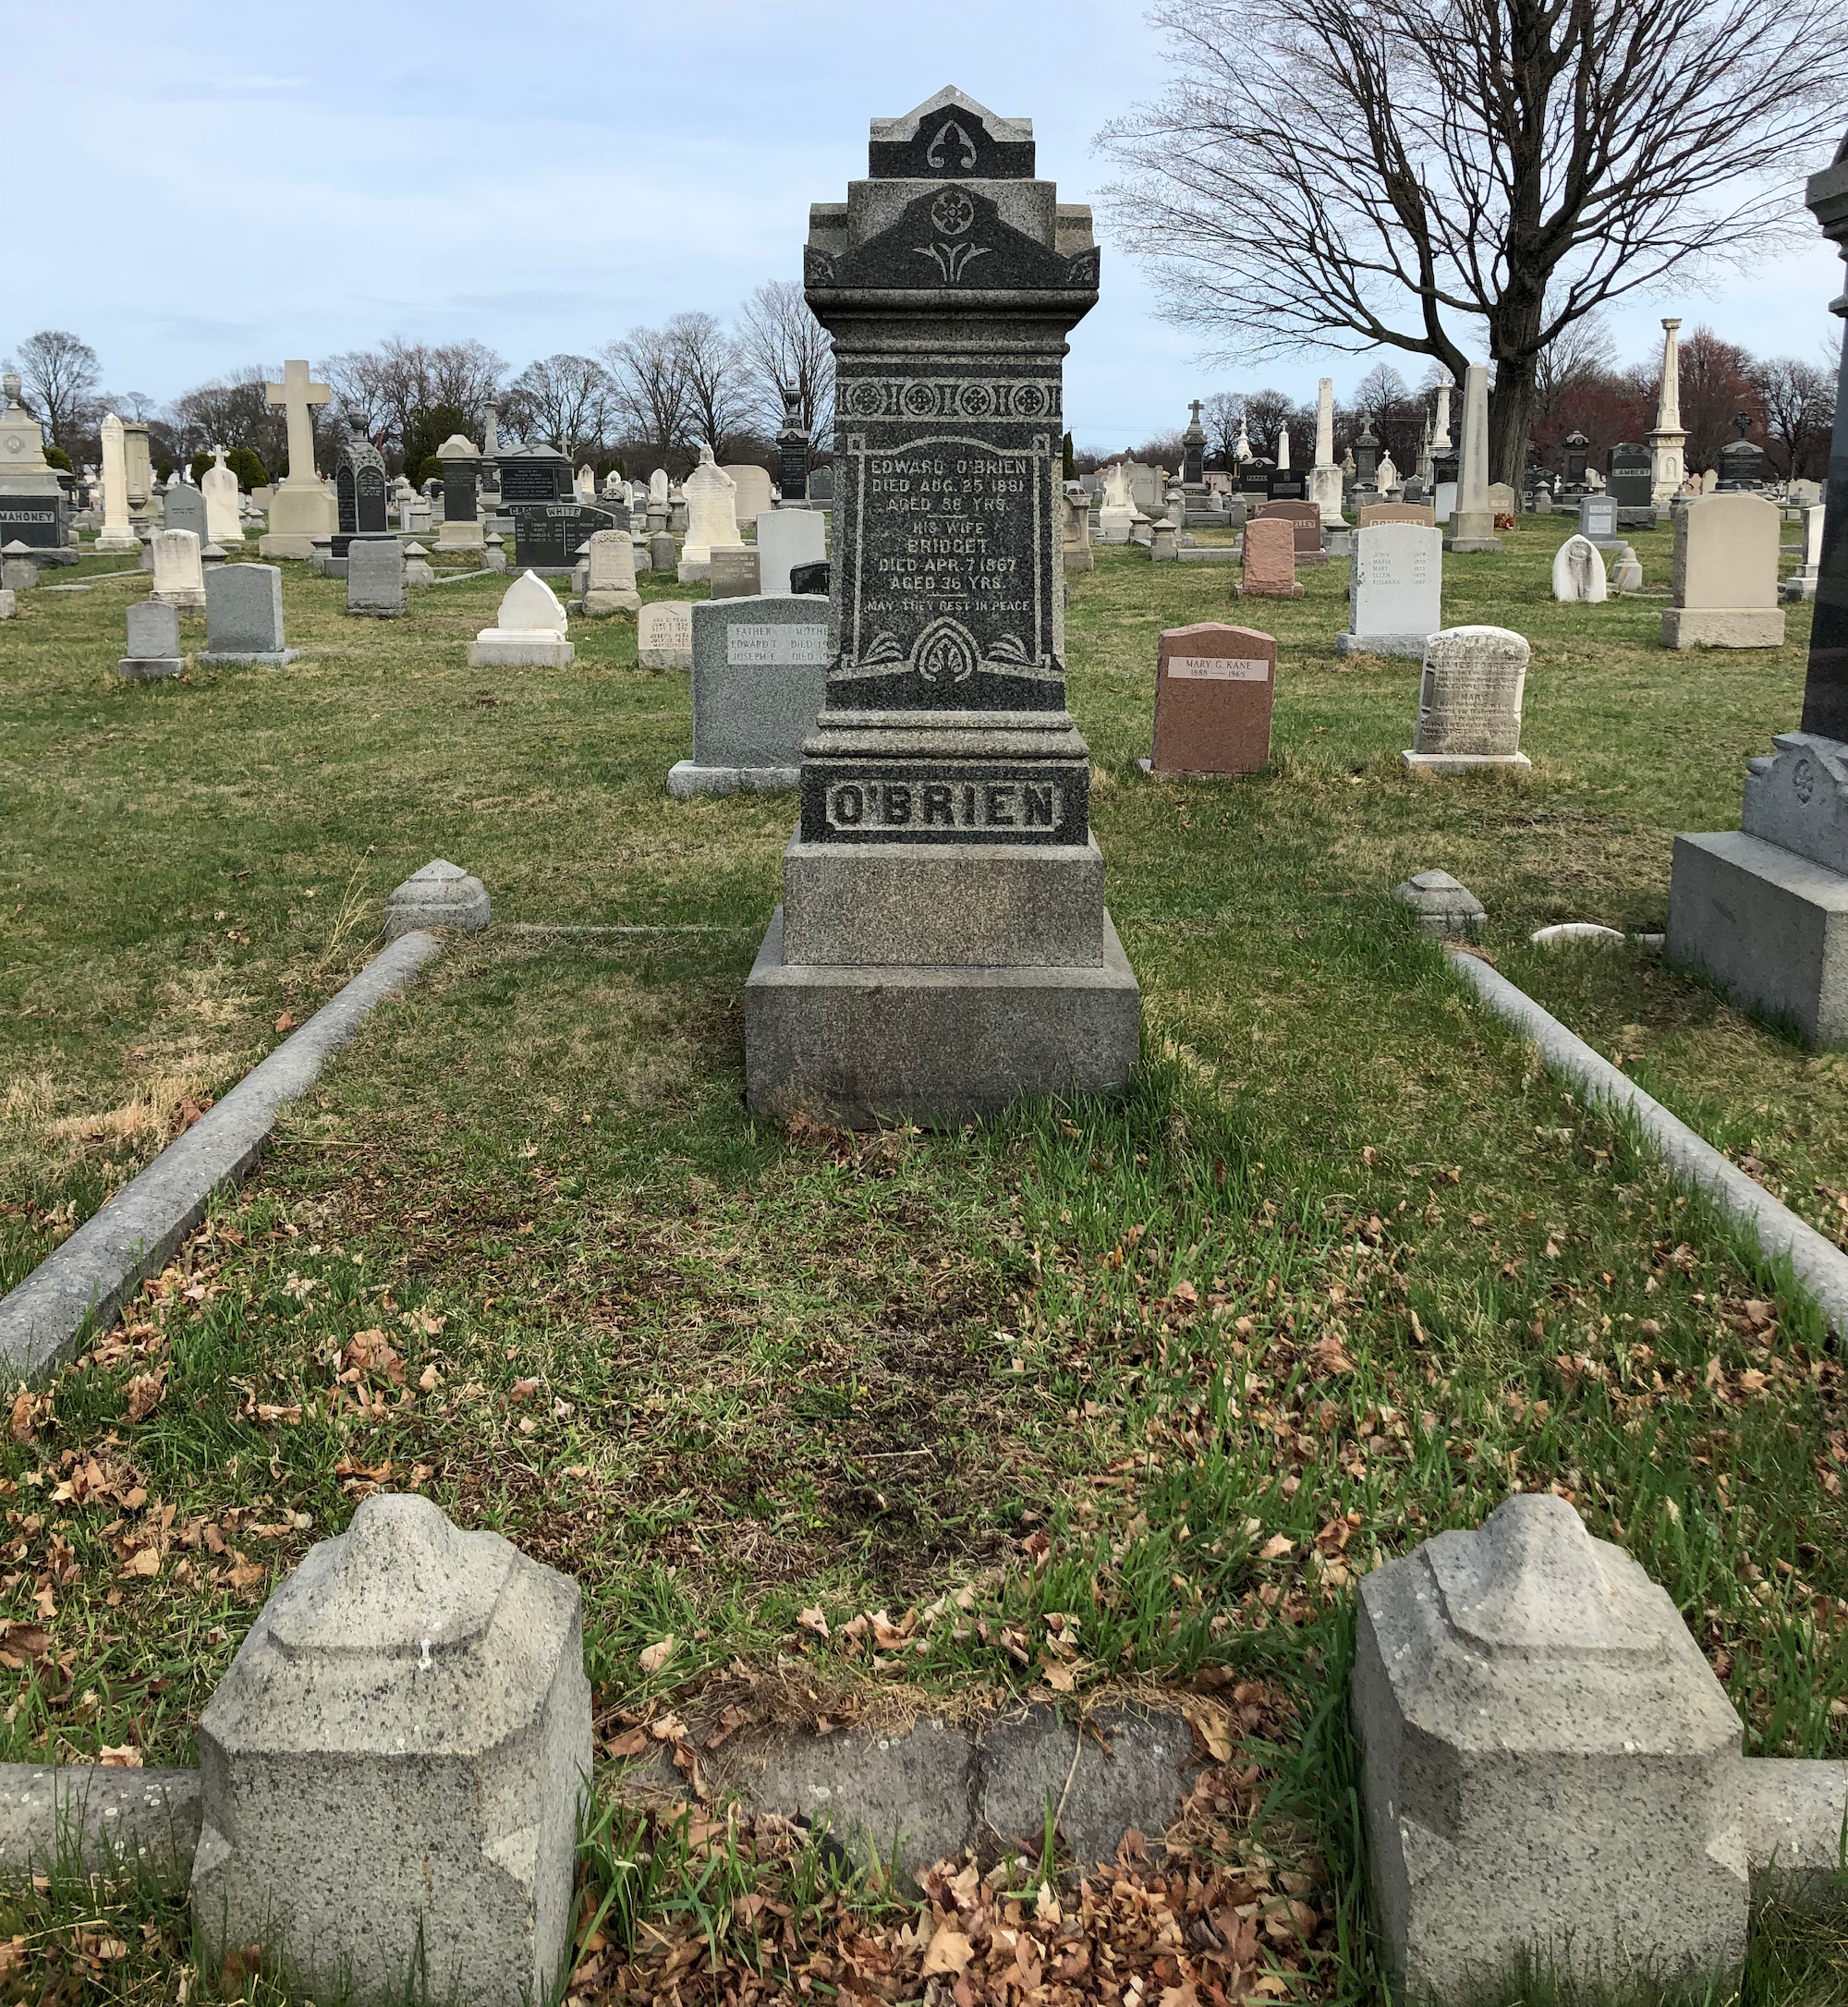
\includegraphics[width=\textwidth]{edward_obrien_grave_wide}
	\caption{Edward O'Brien\index{O'Brien!Edward/Edmund\string\textsuperscript{2}} family plot at Holy Cross Cemetery, Malden, Middlesex County, Massachusetts.\index{Holy Cross Cemetery}\index{Massachusetts!Malden} Photo by Gavin O'Brien, 14 April 2019.}
\end{figure}

\begin{table}[ht]
	\centering
	\caption{Holy Cross Cemetery\index{Holy Cross Cemetery}\cite{HolyCrossPlotMichael} \\
		Malden, Middlesex County, Massachusetts\index{Massachusetts!Malden}
		28 North Monument Path, Grave 27 West (no marker)}
	\begin{tabular}{|l|l|}
		\hline
		\textbf{Name} & \textbf{Burial Date} \\
		\hline
		Mary O'Brien\index{O'Brien!Mary\textsuperscript{3} (1875--1875)} & 21 Nov 1875 \\
		\hline
		John O'Brien\index{O'Brien!John Joseph\textsuperscript{3} (1876--1881)} & 22 Sep 1881 \\
		\hline
		Edward F.\ O'Brien\index{O'Brien!Edward William\textsuperscript{4} (1884--1887)} & 27 Apr 1887 \\
		\hline
		Michael O'Brien\index{O'Brien!Michael\textsuperscript{2}} & 26 Jun 1891 \\
		\hline
		Nellie Wickens\index{Wickens!Nellie\textsuperscript{4}} & 13 Jul 1893 \\
		\hline
		Frank J.\ O'Brien\index{O'Brien!Francis Joseph\textsuperscript{3}} & 04 May 1914 \\
		\hline
		Mary G.\ O'Brien\index{Field!Mary}\index{O'Brien!Mary (Field)} & 09 Jan 1915 \\
		\hline
	\end{tabular}
\end{table}

\begin{table}[ht]
	\centering
	\caption{Catholic Mt.\ Auburn Cemetery\index{Catholic Mt.\ Auburn Cemetery}\cite{BillMcEvoy} \\
		Watertown, Middlesex County, Massachusetts\index{Massachusetts!Watertown}
		Lot 103, Row 2 West (no marker)}
	\begin{tabular}{|l|l|}
		\hline
		\textbf{Name} & \textbf{Burial Date} \\
		\hline
		John O'Brien\index{O'Brien!John\textsuperscript{2}} & 26 Apr 1863 \\
		\hline
		Margaret O'Brien\index{O'Brien!Margaret\textsuperscript{3} (1862--1863)} & 25 Oct 1863 \\
		\hline
		Anna O'Brien\index{O'Brien!Anna\textsuperscript{3}} & 03 Mar 1866 \\
		\hline
		Bridget (Colbert) O'Brien\index{Colbert!Bridget}\index{O'Brien!Bridget (Colbert)} & 21 Oct 1873 \\
		\hline
		James E.\ O'Brien\index{O'Brien!James Edward\textsuperscript{3}} & 12 Apr 1879 \\
		\hline
		Ellen F.\ O'Brien\index{O'Brien!Ellen/Nellie\textsuperscript{3} (1859--1882)} & 01 Oct 1882 \\
		\hline
		Mary O'Brien\index{O'Brien!Mary\textsuperscript{3} (1856--1883)} & 18 Mar 1883 \\
		\hline
		Mary (Mahoney) Bowser\index{Mahoney/Mahony!Mary}\index{O'Brien!Mary (Mahoney)}\index{Bowser!Mary (Mahoney) (O'Brien)} & 18 Nov 1894 \\
		\hline
		Thomas J.\ Bowser\index{Bowser!Thomas} & 27 Mar 1903 \\
		\hline
	\end{tabular}
\end{table}

\begin{table}[ht]
	\centering
	\caption{Mt. Calvary Cemetery\index{Mt.\ Calvary Cemetery}\cite{John3OBrienBurial} \\
		Boston (Roslindale), Suffolk County, Massachusetts\index{Massachusetts!Boston!Roslindale}
		CL1-1 (Half Circle)}
	\begin{tabular}{|l|l|l|}
		\hline
		\textbf{Grave} & \textbf{Name} & \textbf{Burial Date} \\
		\hline
		1A & Catherine J.\ Mahoney\index{Kenney!Catherine Josephine}\index{Mahoney/Mahony!Catherine Josephine (Kenney)} & 13 Mar 1913 \\
		\hline
		1B & Elizabeth F.\ Mahoney\index{Mahoney/Mahony!Elizabeth F.} & 06 Jan 1936 \\
		\hline
		2A & Edward J.\ Mahoney\index{Mahoney/Mahony!Edward} & 15 Jul 1895 \\
		\hline
		2B & Almira L.\ Mahoney\index{Mahoney/Mahony!Almira L.} & 19 May 1910 \\
		\hline
		3A & Agnes P.\ Garvin\index{Garvin!Agnes P.} & 18 Aug 1883 \\
		\hline
		3B & William E.\ Garvin\index{Garvin!William E.} & 25 Oct 1886 \\
		\hline
		3C & Mary A.\ Garvin\index{Garvin!Mary A.} & 12 Jan 1916 \\
		\hline
		4A & Josephine L.\ Mahoney\index{Mahoney/Mahony!Josephine L.} & 17 May 1948 \\
		\hline
		5A & Pauline M.\ Baine\index{O'Brien!Pauline M.\textsuperscript{4}}\index{Baine!Pauline M.\textsuperscript{4} (O'Brien)} & 04 Feb 1967 \\
		\hline
		6A & Mildred L.\ O'Brien\index{O'Brien!Mildred Louise\textsuperscript{4}}\index{French!Mildred Louise\textsuperscript{4} (O'Brien)} & 26 May 1891 \\
		\hline
		6B & Edward O'Brien\index{O'Brien!Edward\textsuperscript{4} (1898--1898)} & 26 Dec 1898 \\
		\hline
		6C & Almira O'Brien\index{O'Brien!Almyra Louise\textsuperscript{4}} & 13 Jul 1902 \\
		\hline
		6D & John J.\ O'Brien\index{O'Brien!John Joseph\textsuperscript{3} (1861--1938)} & 17 May 1938 \\
		\hline
		6E & Emma A.\ O'Brien\index{Mahoney/Mahony!Emma}\index{O'Brien!Emma (Mahony)} & 13 Jul 1950 \\
		\hline
	\end{tabular}
\end{table}

\begin{figure}
	\centering
	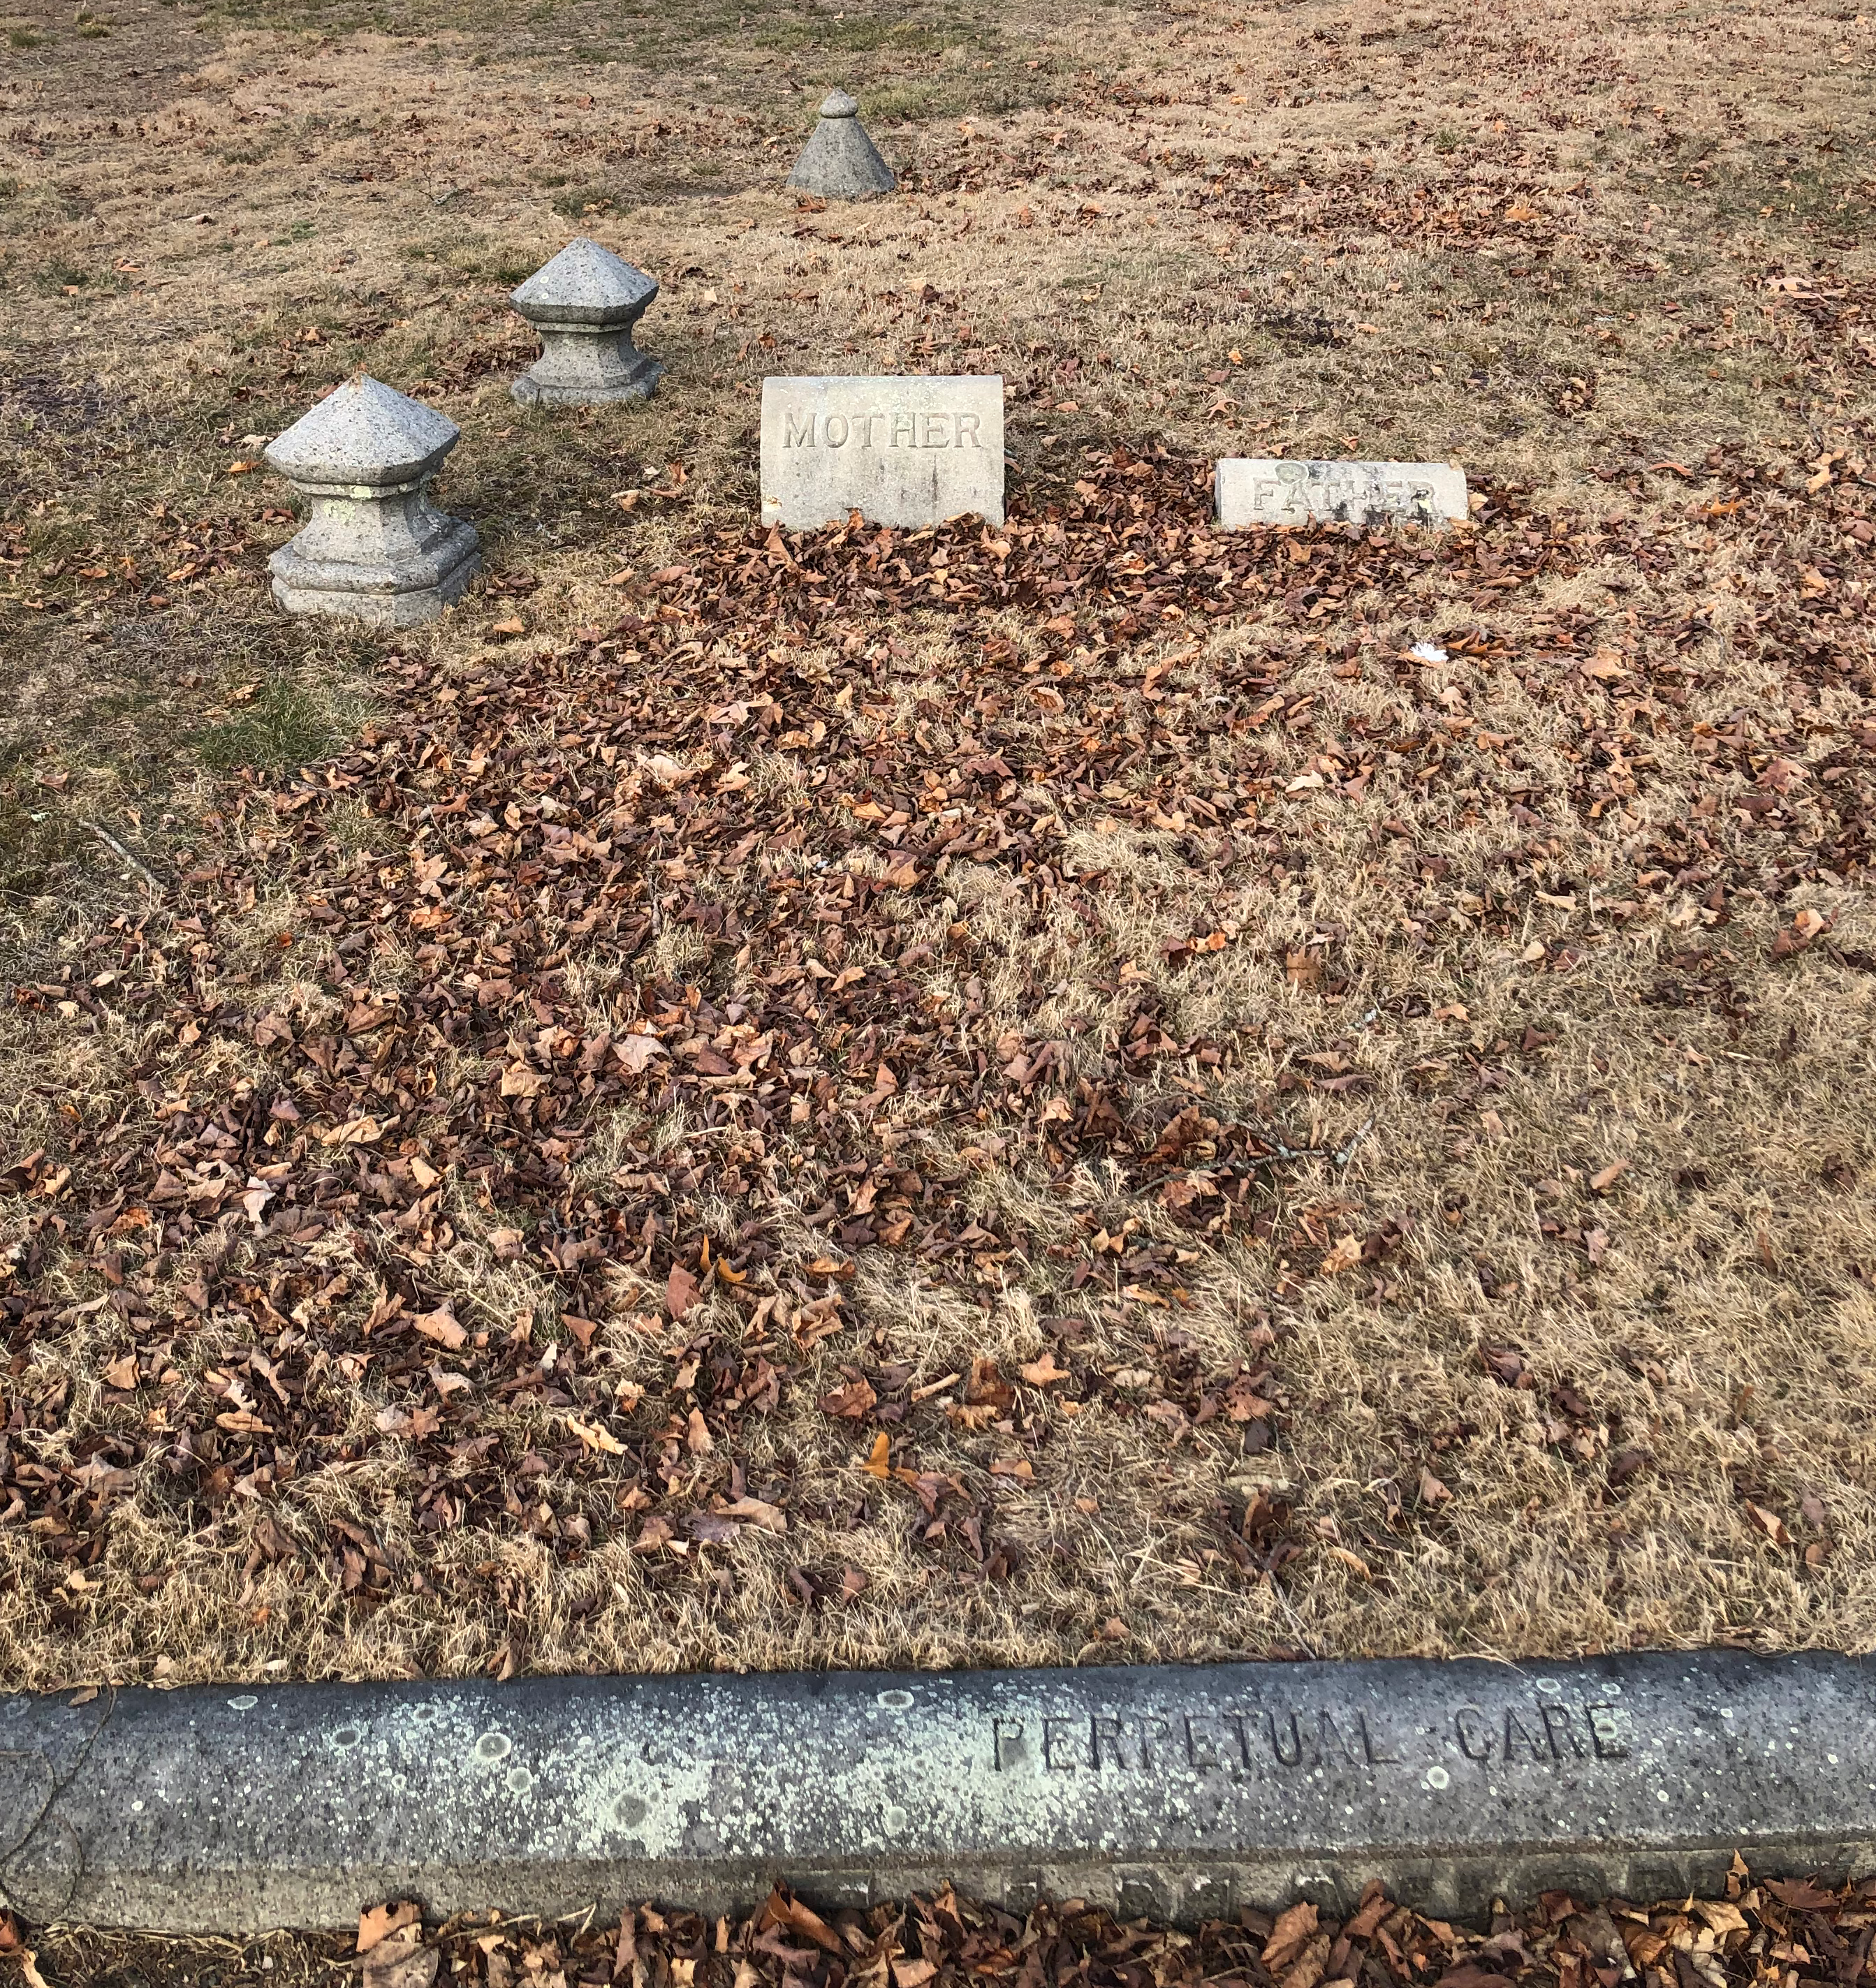
\includegraphics[width=\textwidth]{john_obrien_grave}
	\caption{Mahoney/Mahony family plot,\index{Mahoney/Mahony!family} Mt.\ Calvary Cemetery, Boston (Roslindale), Suffolk County, Massachusetts.\index{Massachusetts!Boston!Roslindale} Photo by Gavin O'Brien, 28 December 2018.}
\end{figure}

\begin{table}[ht]
	\centering
	\caption{Mt.\ Calvary Cemetery\index{Mt.\ Calvary Cemetery}\cite{William3OBrienBurial} \\
		Boston (Roslindale), Suffolk County, Massachusetts\index{Massachusetts!Boston!Roslindale}
		C7-22-22}
	\begin{tabular}{|l|l|}
		\hline
		\textbf{Name} & \textbf{Burial Date} \\
		\hline
		Julia T.\ O'Brien\index{McCarty!Julia T.}\index{O'Brien!Julia T.\ (McCarty)} & 11 Dec 1888 \\
		\hline
		William O'Brien\index{O'Brien!William\textsuperscript{3}} & 29 Oct 1889 \\
		\hline
		Nellie L.\ O'Brien\index{O'Brien!Ellen/Nellie Louise\textsuperscript{4}} & 15 Jun 1926 \\
		\hline
	\end{tabular}
\end{table}

\begin{figure}
	\centering
	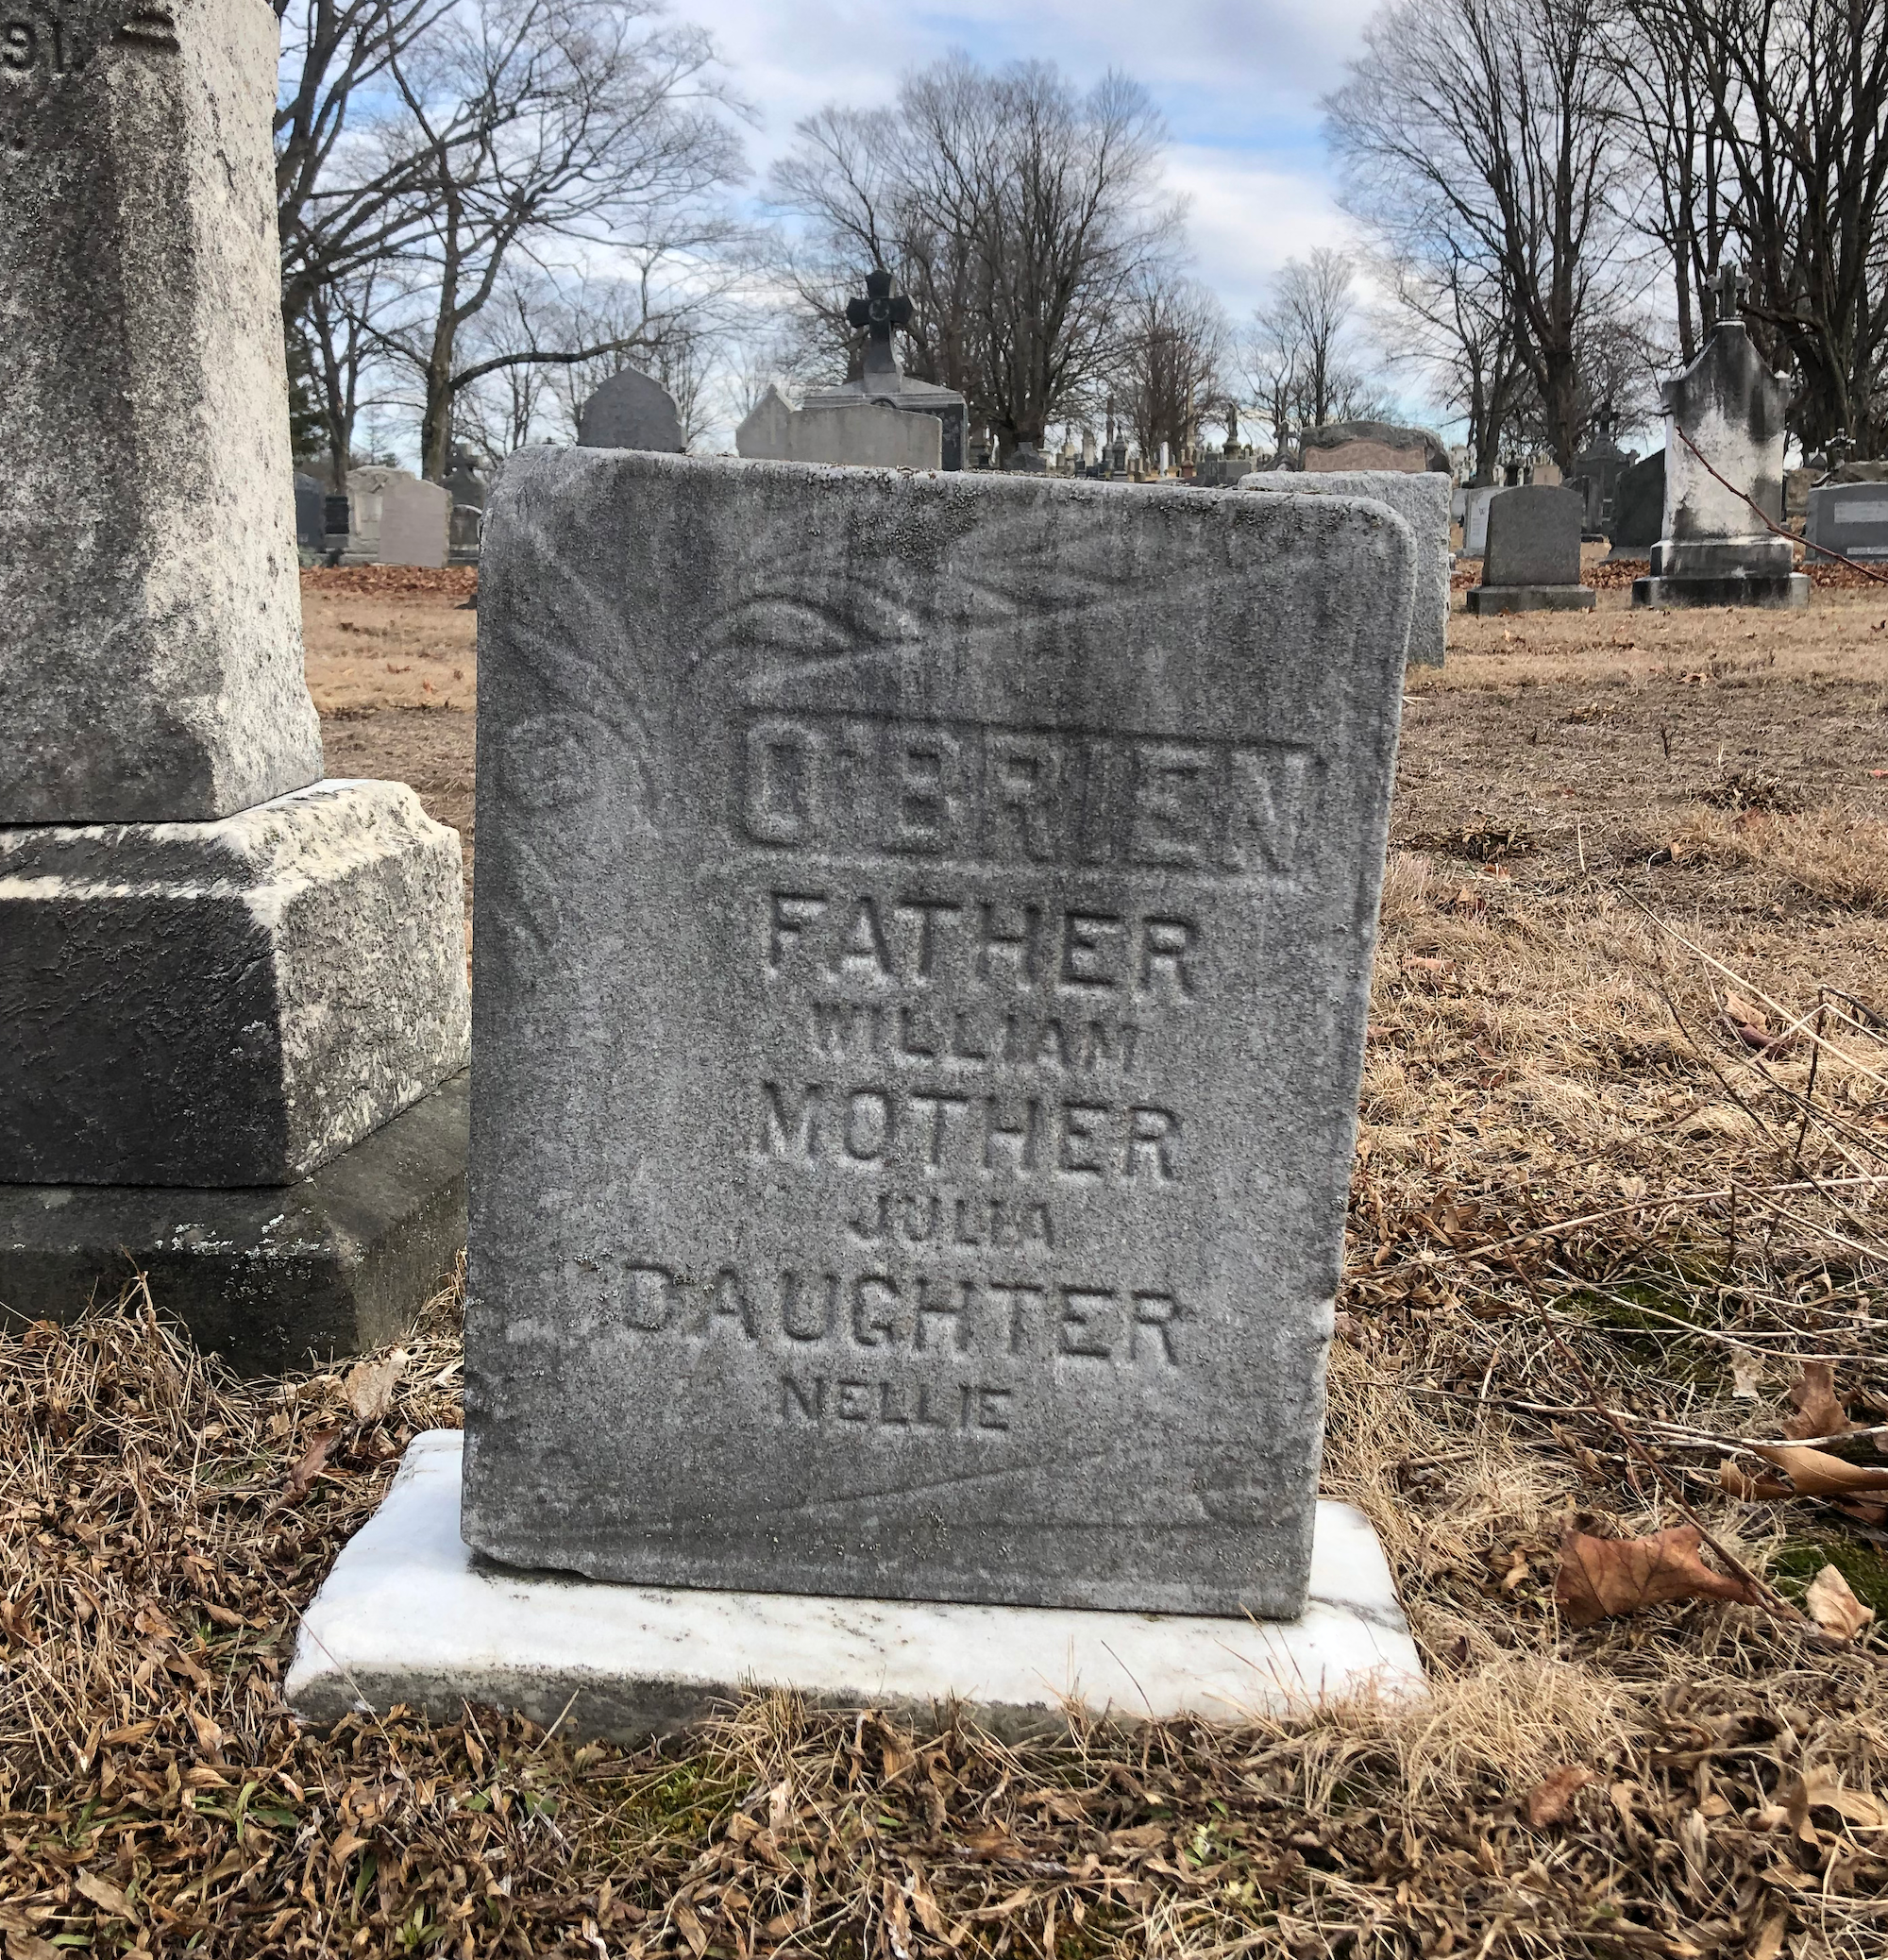
\includegraphics[width=\textwidth]{william_obrien_grave}
	\caption{William O'Brien\index{O'Brien!William\string\textsuperscript{2}} grave, Mt.\ Calvary Cemetery,\index{Mt.\ Calvary Cemetery} Boston (Roslindale), Suffolk County, Massachusetts.\index{Massachusetts!Boston!Roslindale} Photo by Gavin O'Brien, 12 April 2019.}
\end{figure}

\chapter{List of Persons}
\begin{enumerate}
	\item \label{per:William1OBrien} William\textsuperscript{1} O'Brien
	\item \label{per:John2OBrien} John\textsuperscript{2} O'Brien
	\item \label{per:Abigail2OBrien} Abigail\textsuperscript{2} (O'Brien) Dooley
	\item \label{per:Edward2OBrien} Edward\textsuperscript{2} O'Brien
	\item \label{per:Mary2OBrien} Mary\textsuperscript{2} (O'Brien) Ward
	\item \label{per:Michael2OBrien} Michael\textsuperscript{2} O'Brien
\end{enumerate}

Ann\textsuperscript{2} (O'Brien) Dailey

\begin{thebibliography}{999}
	\addcontentsline{toc}{chapter}{\bibname}
	\raggedright
	\small

% Appendices

%% Further Research

\bibitem{John3OBrien1916:4}
W. A. Greenough Co., compilers, \textit{1916 Medford Directory} (Boston: W. A. Greenough \& Co., 1916), p.\ 219, entry for John J O'Brien; viewed at ``U.S. City Directories, 1822-1995,'' database with images, \textit{Ancestry.com} (\url{https://www.ancestry.com/search/collections/2469/} : viewed on 13 Apr 2020), Massachusetts > Medford > 1916 > Medford, Massachusetts, City Directory, 1916 > image 217.\\
``O'Brien John J picture frame mfr 69 Cornhill B 45 Court''\\
John O'Brien appears in the next available Medford city directory for 1918 with no business or profession listed. In the 1920 census his occupation is listed as ``none.''

%% Cemetery Plots

\bibitem{DianaBerberenaLetter1:3}
Diana Berberena, Catholic Cemetery Association of the Archdiocese of Boston, letter to Gavin E.\ O'Brien, dated 27 May 2019. This letter includes burial information for two individuals. William O'Brien, buried 12/30/[1856], age 76 years into O'Brien Family Grave G W124 Range N17 west, owner Edward O'Brien. Mary Ann O'Brien, buried 11/1852, age 1 month, 12 days old.

\bibitem{HolyCrossPlotEdward:2}
The Catholic Cemetery Association of the Archdiocese of Boston, Owner Profile, owner ID C15-61458 (Edward O'Brien) at Holy Cross Cemetery, printed 18 Jul 2019.

\bibitem{HolyCrossPlotMichael}
The Catholic Cemetery Association of the Archdiocese of Boston, Owner Profile, owner ID C15-84952 (Michael O'Brien) at Holy Cross Cemetery, printed 18 Jul 2019.ƒ

\bibitem{HolyCrossPlotFernald}
The Catholic Cemetery Association of the Archdiocese of Boston, Owner Profile, owner ID C15-86405 (Robert Fernald) at Holy Cross Cemetery, printed 22 Jan 2021.

\bibitem{BillMcEvoy:5}
Bill McEvoy, compiler, ``Sand Banks Cemetery Project,'' Excel spreadsheet of plot locations, sourced from burial books and cemetery lot cards of the Catholic Archdiocese of Boston; accessed at \textit{The Historical Society of Watertown} (\url{http://historicalsocietyofwatertownma.org/HSW/} : viewed on 31 Mar 2020), Resources > Sand Banks Cemetery Project > downloadable Excel spreadsheet.

\bibitem{John3OBrienBurial:3}
Mt.\ Calvary Cemetery, Boston, Suffolk County, Massachusetts, printout of Mahoney plot (CL1-1-6D) originally given to Michael O'Brien and verified by Gavin O'Brien at the cemetery office, 28 Dec 2018.

\bibitem{William3OBrienBurial}
Mt.\ Calvary Cemetery, Boston, Suffolk County, Massachusetts, listing for William O'Brien plot (location C7-22-22, owner ID 14237) printed at the cemetery office for Gavin O'Brien on 12 April 2019.

\end{thebibliography}

\backmatter


% \section{Credits}
\raggedright
\setlength{\parskip}{1em}

\ref{fig:IrelandMap} \copyright OpenStreetMap contributors with data available under the \href{https://www.openstreetmap.org/copyright}{Open Database License}.

\ref{fig:WatergrasshillMap} Ordnance Survey Ireland, map series ``Historic 6'' First Edition B\&W (1829--41)'', scale 1:5,000, map sheet CK053

\ref{fig:FamineRelief} The \textit{Constitution}, RLFC 3/2/6/21 (hand-written); ``Famine Relief Commission Papers, 1845–1847,'' RFLC3/2, Incoming Letters: Baronial Sub-series, The National Archives of Ireland, Dublin Ireland;
accessed at ``Ireland, Famine Relief Commission Papers, 1844-1847,'' \textit{Ancestry.com} (\url{https://www.ancestry.com/search/collections/1772/} : viewed on 7 Aug 2020), Incoming Letters: Baronial Sub-series (RLFC3/2/) > 1 - 200 > 21 > image 252.

\ref{fig:Clipper} Thomas Goldsworthy Dutton, ``Clipper barque Spirit of the Age,'' Royal Museums Greenwich (\url{https://commons.wikimedia.org/wiki/File:Clipper_barque_Spirit_of_the_Age,_PY0633.jpg}).

\ref{fig:ThomasBaker} U.S. National Archives and Records Administration (NARA), ``Passenger lists of vessels arriving at New York, 1820-1897,'' NARA microfilm publication M237, roll 81, July 3-27, 1849, list no.\ 882, entries for Mary O'Brien and Michael O'Brien; accessed at ``New York Passenger Lists, 1820-1891,'' database with images, \textit{FamilySearch} (\url{https://familysearch.org/ark:/61903/3:1:939V-5P37-F7} : viewed on 19 Sep 2020), 081 - 3 Jul 1849-27 Jul 1849 > image 123.

\ref{fig:Chasca} ``Registers of Passengers Arriving in Massachusetts Ports 1848-1891,'' Massachusetts State Archives, HS 3.02 1990X, record of 27 Jun 1851, vessel \textit{Chascay}, entries for Edmund O'Brien and family; accessed at ``Massachusetts, United States Records,'' images, FamilySearch (\url{https://www.familysearch.org/ark:/61903/3:1:3Q9M-CSVN-998J-W} : viewed on 11 Nov 2020), image 793.\\
On this page the ship name is written as ``Chascay'' but on the previous pages appears as ``Chasca.''

\ref{fig:StMarys} Josiah Johnson Hawes, ``Old St.\ Mary's Church, Endicott ad Cooper Sts.,''\index{St.\ Mary's of the Sacred Heart (church)} photograph, 1860, Boston Public Library Arts Department (\url{https://ark.digitalcommonwealth.org/ark:/50959/c821h611m}).

\ref{fig:OysterTongers} Jacob Gayer, ``People tonging oysters near Nanticoke,'' photograph, National Geographic, image ID 1238550, used with permission.

\ref{fig:EastBostonMap} Massachusetts, Suffolk County Register of Deeds, \textit{Atlas of East Boston}, 1892, vol.\ 9, p.\ 14; accessed at Suffolk County Register of Deeds (\url{https://massrods.com/suffolk/suffolk-county-atlas/suffolk-county-atlas-pages/} : viewed on 4 Apr 2020), Research > Suffolk County Atlases > East Boston 1892 > Page 14.

\ref{fig:PictureFrameLabel} Label for John J.\ O'Brien,\index{O'Brien!John Joseph\string\textsuperscript{3} (1861--1938)|bb} picture frames,\index{picture frame manufacturing} 69 Cornhill, Boston, Mass., undated. Historic New England, Ephemera Collection, GUSN-265637 (\url{http://gusn.us/265637}).

\ref{fig:FrameStore} Detail from ``Crosswalk on Corn Hill opposite Franklin Avenue, looking west, sect. 8 1/2, Boston, Mass.,'' photograph, Boston Transit Commission, 14 Apr 1897, John Booras collection of plate glass negatives, Historic New England, GUSN-318238 (\url{http://gusn.us/318238}) 

\ref{fig:RobertFernald} ``Robert A.\ Fernald, Veteran Tow Boat\index{tow boat} Captain,\index{captain} Dead,'' \textit{The Boston Globe}, 15 Jun 1917, p.\ 15.

\ref{fig:EdwardOBrienGrave} Photo by Gavin O'Brien, 14 April 2019.

\ref{fig:FernaldGrave} Photo by Gavin O'Brien, 14 April 2019.

\ref{fig:MahoneyPlot} Photo by Gavin O'Brien, 19 January 2021.

\ref{fig:WilliamOBrienGrave} Photo by Gavin O'Brien, 19 January 2021.

\indexprologue{Note: \textbf{bold} page numbers indicate the individual's main profile. Superscripted numbers show the individual's generation, starting with 1 for the oldest generation (William\textsuperscript{1} O'Brien).}
\printindex

\end{document}

